% 高一127_南汇一中_期中.tex
%   —— 高一上数学“2026-2027 年南汇一中高一上期中”（试卷版/答案版）
% 试卷版：xelatex 高一127_南汇一中_期中.tex
% 答案版：xelatex "\def\isanswer{1}% 高一127_南汇一中_期中.tex
%   —— 高一上数学“2026-2027 年南汇一中高一上期中”（试卷版/答案版）
% 试卷版：xelatex 高一127_南汇一中_期中.tex
% 答案版：xelatex "\def\isanswer{1}% 高一127_南汇一中_期中.tex
%   —— 高一上数学“2026-2027 年南汇一中高一上期中”（试卷版/答案版）
% 试卷版：xelatex 高一127_南汇一中_期中.tex
% 答案版：xelatex "\def\isanswer{1}% 高一127_南汇一中_期中.tex
%   —— 高一上数学“2026-2027 年南汇一中高一上期中”（试卷版/答案版）
% 试卷版：xelatex 高一127_南汇一中_期中.tex
% 答案版：xelatex "\def\isanswer{1}\input{高一127_南汇一中_期中.tex}"
% 紧凑版：xelatex "\def\iscompact{1}\input{高一127_南汇一中_期中.tex}"
%
% 原始材料：微信公众号“魔都数学加油站”文章，作者破晓，2026-11-11 18:35 发布；
% 连载“27学年高一127”，原文标题“27学年高一127——2026-2027年上海市南汇一中高一上期中”；
% 原文链接：https://mp.weixin.qq.com/s/nozIwRgeWSKPCPSiqfCm2Q。
% 正文为 9 张 PNG 页（01、02、03、09 为 2560×3620，04、05、06、07、08 为 4762×6735），
% 题目下印有【解析】，为讲评版。题目、解析均据原图转录；
% 卷面粉红色水印“魔都数学加油站”及公众号页脚未录入。全卷仅第 4 题一幅插图。
% 第 09 页只有一行“对称中心为(-1,1).”及水印，是第 08 页末行的续尾页。
%
% 卷首标题：原卷印作“2026-2027 年南汇一中高一上期中”（公众号标题中的“上海市”
% 卷面标题行没有，本稿照卷面），年份区间按全稿惯例排 en dash；原卷未印副标题，
% 本卷为期中卷、跨三章，按题目内容标为“集合与常用逻辑用语、不等式、函数”
% （第 4/5/6/16/18/20 题为集合与常用逻辑用语，第 8/10/11/12/14/17 题为不等式，
% 第 3/7/9/13/15/19/21 题为函数；与 106、125 同为期中复习卷，口径相同）。
%
% 与原卷的排版差异：
%   ① 原文从第 3 题起，填空题编号为 3—12、选择题为 13—16、解答题为 17—21，本稿保留原题号；
%   ② 原卷每题下直接印【解析】，本稿按全稿惯例置于答案版；四道选择题答案均在解析末句
%      “故选 …”，括号内留空、不另提 \ans{}；全卷无只印【答案】或括号内答案的题；
%   ③ 原卷未印副标题，本稿按“知识模块”口径补出；
%   ④ 原卷填空横线按全稿惯例排为 \blankline[4.4em]；选择题括号排 \mbox{（\quad）}、
%      选项段前按惯例加 \keepwithprev；解答题不留作答区（原卷为讲评版，与 109—125 同）；
%      第 21 题 (1) 的四处填空横线亦排 \blankline[4.4em]；
%   ⑤ 原卷数集排斜体 $R$，按全稿惯例改 \R；绝对值排 \lvert…\rvert，集合描述竖线排 \mid；
%      补集记号照原卷上划线排 \overline{A}；不等号一律 \leqslant / \geqslant；
%   ⑥ 第 4 题插图原在题干右侧，本稿按全稿惯例移至题干之后居中排（取原卷截图、
%      去粉色水印后 2× LANCZOS 放大，存 figures/gao127_q4.png），三版都出；
%      并在该题 \item 前加 \needvspace{} 守卫，把题干与插图整块推走；
%   ⑦ 原卷子题编号 (1)(2)(3) 与括号按全稿惯例排；“（单位：万元）”“（写解析式）”
%      用全角括号，第 21 题 (3) 解析“(舍去)”用半角括号，均照录；
%   ⑧ 第 09 页仅一行“对称中心为(-1,1).”为第 08 页末行之续尾，本稿按原卷印刷行
%      另起一条 \step，置于答案版最后一题解析之末。
%
% 子集符号：第 18 题 (1) 解析 $A\subseteq B$、第 20 题 (2) 解析 $A\subseteq B$ 均印有
%   下划线，照录 \subseteq；全卷无 \subset。回原图放大逐处确认。
%
% 判别式字形：本卷 5 处判别式（第 5 题解析 cases 内 $\triangle=9+8(a-1)=0$、
%   第 12 题解析 cases 内 $\triangle=16m^2-4m>0$、第 18 题① $\triangle=4(a+1)^2-4(a^2-1)<0$、
%   第 21 题 (2) cases 内 $\triangle=(-a)^2-4\times2\times2\leqslant0$、
%   第 21 题 (3) $\triangle=\left(2\log_2\frac{2a}{a+1}\right)^2-\cdots=0$）均排等边扁三角，
%   照录 \triangle；逐处回原图全分辨率放大确认，无高三角 $\Delta$（与 高一26 排 $\Delta$ 不同）。
%
% 原卷存疑照录：
%   第 6 题题干作“则实数 $m$ 的取值范围是为____”（“是为”叠用，疑衍一字），照录；
%   第 12 题题干“试探究 $x_1+x_2, x_1x_2, x_1^2+x_2^2, \frac1{x_1}+\frac1{x_2}$ 的值，
%     则 $4x_1+x_2$ 的最小值为____”与后文衔接突兀，照录；
%   第 13 题解析 B 作“$(\log_a M)^N\neq N\log_a M=log_a M^n$”，后一 log 为斜体、
%     指数作小写 $n$，与前式 $N\log_a M$ 及题干 $N$ 不一致，照录；
%   第 13 题解析 A、B、C 三步句末用“；”，D 步句末用“.”，标点不一致，照录；
%   第 15 题解析“故 $BD$ 错误.”两选项字母连写、无顿号，照录；
%   第 7 题题干及解析用“图像”，第 15 题 B、C 及解析用“图象”，全卷两种写法混用，照录未统一；
%   第 21 题 (3) 题干“求出 $a$ 值”（通常作“求出 $a$ 的值”），照录；
%   第 21 题 (3) 解析“解得 $a=1$，$\log_2\frac{2a}{a+1}=6$，解得 $a=-\frac{32}{31}$(舍去)，
%     所以 $a=1$”两个“解得”并列、且舍去值用半角括号，照录；
%   第 09 页“对称中心为(-1,1).”用半角括号与半角句点，照录；
%   第 8 题解析“若 $a\leqslant0$，则关于 $x$ 的不等式 $ax^2-3x+2<0$ 的解集不是空集；”
%     未给理由直接断言，照录；
%   第 18 题 (1) 由 $A\subseteq B$ 直接得 $A=B$，照录。
%
% 行数核对：逐题数 \step 条数，合计 95 条（Q3：1；Q4：2；Q5：2；Q6：3；Q7：2；
% Q8：5；Q9：1；Q10：4；Q11：5；Q12：7；Q13：5；Q14：2；Q15：3；Q16：7；
% Q17：2；Q18：8；Q19：10；Q20：7；Q21：19），与原卷印刷行逐题相等
% （cases 块作一个印刷行计；Q21 第 19 行为第 09 页续尾）。全卷 19 题均印【解析】，
% 无只印【答案】或括号内答案的题，故 \ans{} 为 0；四道选择题括号内留空、不另提 \ans{}。
%
\documentclass[a4paper,11pt]{article}
\usepackage{common}

\begin{document}

\examtitlest[3]{2026--2027 年南汇一中高一上期中}{集合与常用逻辑用语、不等式、函数}

\bigsec{一、填空题}

\begin{enumerate}
\setcounter{enumi}{2}

\item 把 $\sqrt[4]{a\sqrt a}(a>0)$ 化成有理数指数幂的形式为\blankline[4.4em].

\ifanswer
\solbegin
\step{$\sqrt[4]{a\sqrt a}=(a\cdot a^{\frac12})^{\frac14}=a^{\frac38}$.}
\solend
\fi

\needvspace{6.5cm}
\item 已知集合 $A=\{x\mid 1<x<2\}$, $B=\left\{x\mid 0<x<\frac32\right\}$, 则如图阴影部分表示的集合是\blankline[4.4em].

\begin{center}
% 图取原卷截图（第 1 页题干右侧）、去水印后 2× LANCZOS 放大，本稿移至题干之后
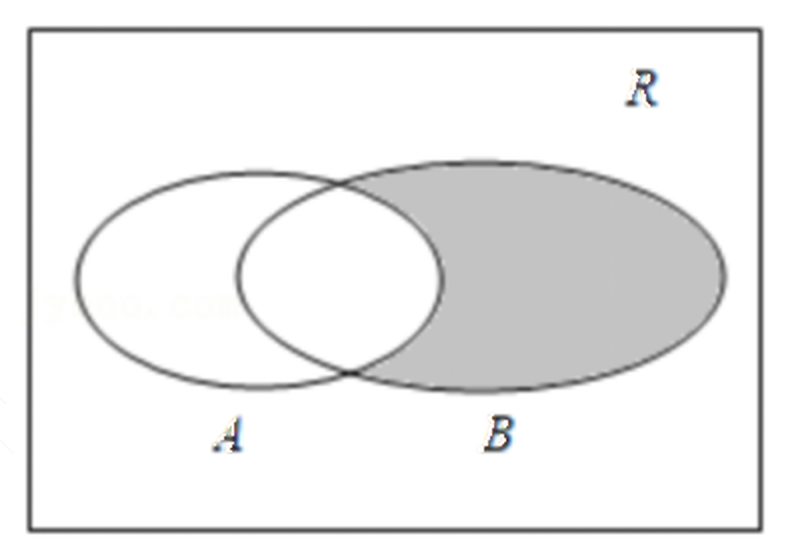
\includegraphics[width=0.36\textwidth]{figures/gao127_q4.png}
\end{center}

\ifanswer
\solbegin
\step{已知 $\R$ 是实数集，集合 $A=\{x\mid 1<x<2\}$, $B=\left\{x\mid 0<x<\frac32\right\}$,}
\step{阴影部分表示的集合是 $\overline A\cap B=\{x\mid 0<x\leqslant1\}$，即 $(0,1]$.}
\solend
\fi

\item 若集合 $\{x\mid (a-1)x^2+3x-2=0\}$ 有且仅有两个子集，则实数 $a$ 的值为\blankline[4.4em].

\ifanswer
\solbegin
\step{由题意得 $\{x\mid (a-1)x^2+3x-2=0\}$ 为单元素集，}
\step{所以 $a-1=0$ 或 $\begin{cases}a-1\neq0\\\triangle=9+8(a-1)=0\end{cases}$，所以 $a=1$ 或 $a=-\frac18$.}
\solend
\fi

\item 已知条件 $\alpha:x\leqslant m$，条件 $\beta:x^2-x\leqslant0$，若 $\alpha$ 是 $\beta$ 的必要条件，则实数 $m$ 的取值范围是为\blankline[4.4em].

\ifanswer
\solbegin
\step{不等式 $x^2-x\leqslant0$ 的解集为 $[0,1]$，}
\step{因为条件 $\alpha:x\leqslant m$，条件 $\beta:x^2-x\leqslant0$，且 $\alpha$ 是 $\beta$ 的必要条件，}
\step{所以集合 $[0,1]$ 是集合 $(-\infty,m]$ 的子集，得 $m\geqslant1$，实数 $m$ 的取值范围是 $[1,+\infty)$.}
\solend
\fi

\item 已知 $\alpha\in\{-2,-1,-\frac12,0,1,2\}$，若幂函数 $y=x^\alpha$ 在 $(0,+\infty)$ 是严格减函数且图像关于 $y$ 轴对称，则 $\alpha=$\blankline[4.4em].

\ifanswer
\solbegin
\step{幂函数 $y=x^\alpha$ 在 $(0,+\infty)$ 是严格减函数，则 $\alpha<0$，且图像关于 $y$ 轴对称，}
\step{则函数为偶函数，故 $\alpha=-2$.}
\solend
\fi

\item 若关于 $x$ 的不等式 $ax^2-3x+2<0$ 的解集不是空集，则实数 $a$ 的取值范围是\blankline[4.4em].

\ifanswer
\solbegin
\step{若 $a>0$，关于 $x$ 的不等式 $ax^2-3x+2<0$ 的解集不空，}
\step{所以一元二次方程 $ax^2-3x+2=0$ 的判别式大于零，}
\step{即 $(-3)^2-8a>0\Rightarrow a<\frac98$，结合 $a>0$ 得 $0<a<\frac98$；}
\step{若 $a\leqslant0$，则关于 $x$ 的不等式 $ax^2-3x+2<0$ 的解集不是空集；}
\step{综上，实数 $a$ 的取值范围是 $\left(-\infty,\frac98\right)$.}
\solend
\fi

\item 设 $\log_{18}2=a$，则 $\log_2 3$ 可用 $a$ 表示为\blankline[4.4em].

\ifanswer
\solbegin
\step{因为 $\log_{18}2=\frac{\log_2 2}{\log_2 18}=\frac1{1+2\log_2 3}=a$，则 $\log_2 3=\frac{1-a}{2a}$.}
\solend
\fi

\item 若关于 $x$ 的不等式 $ax^2+bx+c>0$ 解集为 $\left(-\frac12,3\right)$，则关于 $x$ 的不等式 $cx^2+bx+a<0$ 的解集为\blankline[4.4em].

\ifanswer
\solbegin
\step{由已知得 $a<0$，且 $ax^2+bx+c=a\left(x+\frac12\right)(x-3)$，}
\step{所以 $b=-\frac52 a, c=-\frac32 a$，}
\step{$cx^2+bx+a=-\frac a2(3x-1)(x+2)<0\Leftrightarrow(3x-1)(x+2)<0\Leftrightarrow -2<x<\frac13$，}
\step{故解集为 $\left(-2,\frac13\right)$.}
\solend
\fi

\item 设 $x\in\R$，则方程 $\lvert 2x+3\rvert-\lvert x-2\rvert=\lvert 3x+1\rvert$ 的解集为\blankline[4.4em].

\ifanswer
\solbegin
\step{当 $x\leqslant-\frac32$ 时，原式 $\Leftrightarrow -2x-3+x-2=-3x-1\Leftrightarrow x=2$，不合题意；}
\step{当 $-\frac32<x\leqslant-\frac13$ 时，原式 $\Leftrightarrow 2x+3+x-2=-3x-1\Leftrightarrow x=-\frac13$；}
\step{当 $-\frac13<x\leqslant2$ 时，原式 $\Leftrightarrow 2x+3+x-2=3x+1\Leftrightarrow 1=1$ 即恒成立；}
\step{当 $x>2$ 时，原式 $\Leftrightarrow 2x+3+2-x=3x+1\Leftrightarrow x=2$，不合题意；}
\step{故 $x\in\left[-\frac13,2\right]$.}
\solend
\fi

\item 若关于 $x$ 的不等式 $x^2-4mx+m<0$ 的解集为 $(x_1,x_2)$，若 $x_1>0,x_2>0$，试探究 $x_1+x_2,x_1x_2,x_1^2+x_2^2,\frac1{x_1}+\frac1{x_2}$ 的值，则 $4x_1+x_2$ 的最小值为\blankline[4.4em].

\ifanswer
\solbegin
\step{由题意得方程 $x^2-4mx+m=0$ 有两个相异的正实根 $x_1,x_2$，}
\step{故有 $\begin{cases}\triangle=16m^2-4m>0\\x_1+x_2=4m>0\\x_1\cdot x_2=m>0\end{cases}$，解得 $m>\frac14$，}
\step{则 $x_1^2+x_2^2=(x_1+x_2)^2-2x_1\cdot x_2=16m^2-2m$，$\frac1{x_1}+\frac1{x_2}=\frac{x_1+x_2}{x_1\cdot x_2}=4$，}
\step{则 $4x_1+x_2=\frac14(4x_1+x_2)\left(\frac1{x_1}+\frac1{x_2}\right)=\frac14\left(5+\frac{4x_1}{x_2}+\frac{x_2}{x_1}\right)\geqslant\frac94$，}
\step{当且仅当 $\frac{4x_1}{x_2}=\frac{x_2}{x_1}$ 时，即 $x_2=2x_1$ 时取等号，}
\step{由 $\begin{cases}x_2=2x_1\\\frac1{x_1}+\frac1{x_2}=4\end{cases}$，解得 $\begin{cases}x_1=\frac38\\x_2=\frac34\end{cases}$，于是 $m=x_1\cdot x_2=\frac9{32}\in\left(\frac14,+\infty\right)$，}
\step{即当 $m=\frac9{32}$ 时，$4x_1+x_2$ 取得最小值为 $\frac94$.}
\solend
\fi

\end{enumerate}

\bigsec{二、选择题}

\begin{enumerate}
\setcounter{enumi}{12}

\item 若 $a>0$, $a\neq1$, $M>0$, $N>0$，下列运算正确的是\mbox{（\quad）}

\keepwithprev
A. $\log_a\sqrt[N]{M}=\frac1N\log_a M$\qquad\qquad B. $(\log_a M)^N=N\log_a M$

C. $(\log_a M)\div(\log_a N)=\log_a(M-N)$\qquad\quad D. $\log_a M+\log_a N=\log_a(M+N)$

\ifanswer
\solbegin
\step{对于 $A$，$\log_a\sqrt[N]{M}=\log_a M^{\frac1N}=\frac1N\log_a M$，故 $A$ 正确；}
\step{对于 $B$，$(\log_a M)^N\neq N\log_a M=log_a M^n$，故 $B$ 错误；}
\step{对于 $C$，$(\log_a M)\div(\log_a N)\neq\log_a(M-N)$，故 $C$ 错误；}
\step{对于 $D$，$\log_a M+\log_a N=\log_a MN\neq\log_a(M+N)$，故 $D$ 错误.}
\step{故选 $A$.}
\solend
\fi

\item 下列不等式中正确的是\mbox{（\quad）}

\keepwithprev
A. 若 $a>b$，则 $ac^2>bc^2$\qquad\qquad B. 若 $a<b<0$，则 $a^2<b^2$

C. 若 $1<a<2$ 且 $0<b<3$，则 $1<a+b<5$\qquad D. 若 $\frac1a<1$，则 $a>1$

\ifanswer
\solbegin
\step{$C$ 中 $1+0<a+b<2+3$，即 $1<a+b<5$，正确.}
\step{$A$ 取 $c=0$ 时不成立；$B$ 应为 $a^2>b^2$；$D$ 取 $a=-1$ 时不成立. 故选 $C$.}
\solend
\fi

\item 已知 $y_1=x^3,y_2=x^2$，则下列说法正确的是\mbox{（\quad）}

\keepwithprev
A. $x\in(0,+\infty)$ 时，恒有 $y_1\geqslant y_2$

B. $y_1=x^3$ 与 $y_2=x^2$ 的函数图象仅有唯一交点

C. $x\in(0,1)$ 时，$y_1=x^3$ 图象在 $y_2=x^2$ 图象下方

D. 存在 $x_0\in(1,+\infty)$ 使得 $y_1=y_2$

\ifanswer
\solbegin
\step{$y_1-y_2=x^2(x-1)$，当 $0<x<1$ 时，$y_1<y_2$，故 $C$ 正确，$A$ 错误.}
\step{$y_1=y_2\Leftrightarrow x^2(x-1)=0\Leftrightarrow x=0$ 或 $x=1$，两图象有两个交点，故 $BD$ 错误.}
\step{故选 $C$.}
\solend
\fi

\item 已知非空集合 $A$、$B$ 满足两个条件：(1) $A\cup B=\{1,2,3,4,5,6,7\}$, $A\cap B=\varnothing$；(2) 若 $x\in A$，则 $x+1\in B$，则有序集合对 $(A,B)$ 的个数为\mbox{（\quad）}

\keepwithprev
A. $17$\qquad\qquad B. $18$\qquad\qquad C. $19$\qquad\qquad D. $20$

\ifanswer
\solbegin
\step{当 $A$ 为单元素集合时，有 6 种情况：}
\step{当 $A$ 为双元素集合时，$A=\{1,3\}, A=\{1,4\}, A=\{1,5\}, A=\{1,6\}, A=\{2,4\}$,}
\step{$A=\{2,5\}, A=\{2,6\}, A=\{3,5\}, A=\{3,6\}, A=\{4,6\}$，共 10 种情况；}
\step{当 $A$ 为三元素集合时，$A=\{1,3,5\}, A=\{1,3,6\}, A=\{1,4,6\}, A=\{2,4,6\}$，}
\step{共 4 种情况；}
\step{当 $A$ 为四元素集合时，不成立；}
\step{故有序集合对 $(A,B)$ 的个数为 20，故选 $D$.}
\solend
\fi

\end{enumerate}

\bigsec{三、解答题}

\begin{enumerate}
\setcounter{enumi}{16}

\item 已知 $x,y\in\R$，比较 $x^2+y^2$ 与 $2(2x-y)-5$ 的大小.

\ifanswer
\solbegin
\step{因为 $x^2+y^2-2(2x-y)+5=(x-2)^2+(y+1)^2\geqslant0$，}
\step{所以 $x^2+y^2\geqslant2(2x-y)-5$.}
\solend
\fi

\item 已知集合 $A=\{x\mid x^2+4x=0\}$，$B=\{x\mid x^2+2(a+1)x+a^2-1=0\}$.

(1) 若 $A$ 是 $B$ 的子集，求实数 $a$ 的值；

(2) 若 $B$ 是 $A$ 的子集，求实数 $a$ 的取值范围.

\ifanswer
\solbegin
\step{(1) 因为 $A=\{-4,0\}$，$B=\{x\mid x^2+2(a+1)x+a^2-1=0\}$，又 $A\subseteq B$，}
\step{所以 $A=B$，所以 $\begin{cases}-4+0=-2(a+1)\\-4\times0=a^2-1\end{cases}$，所以 $a=1$；}
\step{(2) 因为 $B$ 是 $A$ 的子集，所以 $B=\varnothing$ 或 $B=\{-4\}$ 或 $B=\{0\}$ 或 $B=\{-4,0\}$，}
\step{① $B=\varnothing$ 时，$\triangle=4(a+1)^2-4(a^2-1)<0$，所以 $a<-1$；}
\step{② $B=\{-4\}$ 时，$\begin{cases}-4+(-4)=-2(a+1)\\-4\times(-4)=a^2-1\end{cases}$，无解；}
\step{③ $B=\{0\}$ 时，$\begin{cases}0+0=-2(a+1)\\0\times0=a^2-1\end{cases}$，所以 $a=-1$；}
\step{④ $B=\{-4,0\}$ 时，由 (1) 得 $a=1$，}
\step{综上，实数 $a$ 的取值范围为 $(-\infty,-1]\cup\{1\}$.}
\solend
\fi

\item 某企业在现有设备下每日生产原先成本 $y$（单位：万元）与日产量 $x$（单位：吨）之间的函数关系式：$y=2x^2+(15-4k)x+120k+8$，近年来各部门都非常重视大气污染防治工作，为了配合环境卫生综合整治，该企业引进了除尘设备，每吨产品的除尘费用为 $k$ 万元，引进除尘设备后，当日产量 $x=1$ 时，总成本（总成本为原先成本和除尘费用之和）为 142 万元.

(1) 求 $k$ 的值；

(2) 求引进除尘设备后日产量为多少时，每吨产品的成本最小，并求出最小值.

\ifanswer
\solbegin
\step{(1) 该企业引进了除尘设备，}
\step{每日生产总成本 $h$（单位：万元）与日产量 $x$（单位：吨）之间的关系为}
\step{$h=2x^2+(15-4k)x+120k+8+kx=2x^2+(15-3k)x+120k+8$，}
\step{当日产量 $x=1$ 时，总成本为 $h=142$ 万元，}
\step{代入得 $2+(15-3k)+120k+8=142\Rightarrow k=1$，}
\step{(2) 由 (1) 得 $h=2x^2+12x+128$，}
\step{所以每吨产品的成本为 $w=\frac{2x^2+12x+128}{x}=2x+\frac{128}{x}+12$}
\step{$\geqslant2\sqrt{2x\cdot\frac{128}{x}}+12=44$，当且仅当 $2x=\frac{128}{x}$，即 $x=8$ 时，取等号，}
\step{所以引进除尘设备后日产量为 8 吨时，每吨产品的成本最小，}
\step{且最小值为 44 万元.}
\solend
\fi

\item 已知集合 $A=\{x\mid \lvert x-a\rvert<2\}$，集合 $B=\left\{x\mid\frac{2x-1}{x+2}<1\right\}$.

(1) 若 $a=2$，求 $A\cup B$；

(2) 若 $A\cap B=A$，求实数 $a$ 的取值范围.

\ifanswer
\solbegin
\step{(1) 若 $a=2$，则 $A=\{x\mid \lvert x-a\rvert<2\}=\{x\mid \lvert x-2\rvert<2\}=\{x\mid 0<x<4\}$，}
\step{由 $\frac{2x-1}{x+2}<1$ 得 $\frac{x-3}{x+2}<0$，即 $(x-3)(x+2)<0$，解得 $-2<x<3$，}
\step{所以 $B=\{x\mid -2<x<3\}$，所以 $A\cup B=\{x\mid -2<x<4\}$；}
\step{(2) 由 (1) 得 $B=\{x\mid -2<x<3\}$，}
\step{$A=\{x\mid \lvert x-a\rvert<2\}=\{x\mid a-2<x<a+2\}$，}
\step{若 $A\cap B=A$，则 $A\subseteq B$，则 $\begin{cases}a-2\geqslant-2\\a+2\leqslant3\end{cases}$，解得 $0\leqslant a\leqslant1$，}
\step{即实数 $a$ 的取值范围为 $[0,1]$.}
\solend
\fi

\item 已知自变量为 $x$ 的函数 $y=\frac{ax+b}{x+a}$，

(1) 若 $a=1$ 且 $b=2$，则函数 $y=\frac{ax+b}{x+a}$ 图像可由幂函数\blankline[4.4em]（写解析式）先沿 $x$ 轴方向\blankline[4.4em]平移\blankline[4.4em]个单位，再沿 $y$ 轴方向向上平移\blankline[4.4em]个单位得到；

(2) 当 $a>0$ 且 $b=-2$ 时不等式 $\frac{ax+b}{x+a}\leqslant\frac{2x^2}{x+a}$ 对 $x>0$ 恒成立，求实数 $a$ 的最大值；

(3) 若 $b=-2$ 且关于 $x$ 的不等式 $x^2\log_2\frac{4(a+1)}a+2x\log_2\frac{2a}{a+1}+\log_2\frac{(a+1)^2}{4a^2}\leqslant0$ 解集是单元素集，求出 $a$ 值，并求出函数 $y=\frac{ax-2}{x+a}$ 的对称中心.

\ifanswer
\solbegin
\step{(1) 已知自变量为 $x$ 的函数 $y=\frac{ax+b}{x+a}$，}
\step{当 $a=1$ 且 $b=2$ 时，$y=\frac{x+2}{x+1}=\frac{x+1+1}{x+1}=1+\frac1{x+1}$，}
\step{由幂函数 $y=\frac1x$，先沿 $x$ 轴方向向左平移一个单位，}
\step{再沿 $y$ 轴方向向上平移一个单位得到；}
\step{(2) 当 $a>0$ 且 $b=-2$ 时不等式 $\frac{ax+b}{x+a}\leqslant\frac{2x^2}{x+a}$ 即 $\frac{ax-2}{x+a}\leqslant\frac{2x^2}{x+a}$ 对 $x>0$ 恒成立，}
\step{因为 $a>0$ 且 $x>0$，所以 $x+a>0$，所以等价于 $ax-2\leqslant2x^2$ 对 $x>0$ 恒成立，}
\step{即 $2x^2-ax+2\geqslant0$ 对 $x>0$ 恒成立，}
\step{因为函数 $g(x)=2x^2-ax+2$ 的对称轴 $x=\frac a4>0$，且 $g(0)=2>0$，}
\step{则 $\begin{cases}\triangle=(-a)^2-4\times2\times2\leqslant0\\a>0\end{cases}$，解得 $0<a\leqslant4$，所以 $a$ 的最大值为 4；}
\step{(3) 关于 $x$ 的不等式 $x^2\log_2\frac{4(a+1)}a+2x\log_2\frac{2a}{a+1}+\log_2\frac{(a+1)^2}{4a^2}\leqslant0$ 解集}
\step{是单元素集，由 $\frac{4(a+1)}a>0$，则 $a>0$ 或 $a<-1$，}
\step{若 $\log_2\frac{4(a+1)}a=0$，则 $\frac{4(a+1)}a=1$，解得 $a=-\frac43$，}
\step{此时不等式为 $6x-6\leqslant0$，解得 $x\leqslant1$，不符合题意，}
\step{若 $\log_2\frac{4(a+1)}a>0$，即 $\frac{4(a+1)}a>1$，解得 $a>0$ 或 $a<-\frac43$，}
\step{则 $\triangle=\left(2\log_2\frac{2a}{a+1}\right)^2-4\log_2\frac{4(a+1)}a\cdot\log_2\frac{(a+1)^2}{4a^2}=0$，}
\step{令 $\log_2\frac{2a}{a+1}=t$，则 $t^2-(3-t)(-2t)=0$，解得 $t=0$ 或 $t=6$，}
\step{当 $\log_2\frac{2a}{a+1}=0$，解得 $a=1$，$\log_2\frac{2a}{a+1}=6$，解得 $a=-\frac{32}{31}$(舍去)，所以 $a=1$，}
\step{则函数 $y=\frac{ax-2}{x+a}$ 即为 $y=\frac{x-2}{x+1}=\frac{x+1-3}{x+1}=1+\frac{-3}{x+1}$，}
\step{对称中心为 $(-1,1)$.}
\solend
\fi

\end{enumerate}

\end{document}
"
% 紧凑版：xelatex "\def\iscompact{1}% 高一127_南汇一中_期中.tex
%   —— 高一上数学“2026-2027 年南汇一中高一上期中”（试卷版/答案版）
% 试卷版：xelatex 高一127_南汇一中_期中.tex
% 答案版：xelatex "\def\isanswer{1}\input{高一127_南汇一中_期中.tex}"
% 紧凑版：xelatex "\def\iscompact{1}\input{高一127_南汇一中_期中.tex}"
%
% 原始材料：微信公众号“魔都数学加油站”文章，作者破晓，2026-11-11 18:35 发布；
% 连载“27学年高一127”，原文标题“27学年高一127——2026-2027年上海市南汇一中高一上期中”；
% 原文链接：https://mp.weixin.qq.com/s/nozIwRgeWSKPCPSiqfCm2Q。
% 正文为 9 张 PNG 页（01、02、03、09 为 2560×3620，04、05、06、07、08 为 4762×6735），
% 题目下印有【解析】，为讲评版。题目、解析均据原图转录；
% 卷面粉红色水印“魔都数学加油站”及公众号页脚未录入。全卷仅第 4 题一幅插图。
% 第 09 页只有一行“对称中心为(-1,1).”及水印，是第 08 页末行的续尾页。
%
% 卷首标题：原卷印作“2026-2027 年南汇一中高一上期中”（公众号标题中的“上海市”
% 卷面标题行没有，本稿照卷面），年份区间按全稿惯例排 en dash；原卷未印副标题，
% 本卷为期中卷、跨三章，按题目内容标为“集合与常用逻辑用语、不等式、函数”
% （第 4/5/6/16/18/20 题为集合与常用逻辑用语，第 8/10/11/12/14/17 题为不等式，
% 第 3/7/9/13/15/19/21 题为函数；与 106、125 同为期中复习卷，口径相同）。
%
% 与原卷的排版差异：
%   ① 原文从第 3 题起，填空题编号为 3—12、选择题为 13—16、解答题为 17—21，本稿保留原题号；
%   ② 原卷每题下直接印【解析】，本稿按全稿惯例置于答案版；四道选择题答案均在解析末句
%      “故选 …”，括号内留空、不另提 \ans{}；全卷无只印【答案】或括号内答案的题；
%   ③ 原卷未印副标题，本稿按“知识模块”口径补出；
%   ④ 原卷填空横线按全稿惯例排为 \blankline[4.4em]；选择题括号排 \mbox{（\quad）}、
%      选项段前按惯例加 \keepwithprev；解答题不留作答区（原卷为讲评版，与 109—125 同）；
%      第 21 题 (1) 的四处填空横线亦排 \blankline[4.4em]；
%   ⑤ 原卷数集排斜体 $R$，按全稿惯例改 \R；绝对值排 \lvert…\rvert，集合描述竖线排 \mid；
%      补集记号照原卷上划线排 \overline{A}；不等号一律 \leqslant / \geqslant；
%   ⑥ 第 4 题插图原在题干右侧，本稿按全稿惯例移至题干之后居中排（取原卷截图、
%      去粉色水印后 2× LANCZOS 放大，存 figures/gao127_q4.png），三版都出；
%      并在该题 \item 前加 \needvspace{} 守卫，把题干与插图整块推走；
%   ⑦ 原卷子题编号 (1)(2)(3) 与括号按全稿惯例排；“（单位：万元）”“（写解析式）”
%      用全角括号，第 21 题 (3) 解析“(舍去)”用半角括号，均照录；
%   ⑧ 第 09 页仅一行“对称中心为(-1,1).”为第 08 页末行之续尾，本稿按原卷印刷行
%      另起一条 \step，置于答案版最后一题解析之末。
%
% 子集符号：第 18 题 (1) 解析 $A\subseteq B$、第 20 题 (2) 解析 $A\subseteq B$ 均印有
%   下划线，照录 \subseteq；全卷无 \subset。回原图放大逐处确认。
%
% 判别式字形：本卷 5 处判别式（第 5 题解析 cases 内 $\triangle=9+8(a-1)=0$、
%   第 12 题解析 cases 内 $\triangle=16m^2-4m>0$、第 18 题① $\triangle=4(a+1)^2-4(a^2-1)<0$、
%   第 21 题 (2) cases 内 $\triangle=(-a)^2-4\times2\times2\leqslant0$、
%   第 21 题 (3) $\triangle=\left(2\log_2\frac{2a}{a+1}\right)^2-\cdots=0$）均排等边扁三角，
%   照录 \triangle；逐处回原图全分辨率放大确认，无高三角 $\Delta$（与 高一26 排 $\Delta$ 不同）。
%
% 原卷存疑照录：
%   第 6 题题干作“则实数 $m$ 的取值范围是为____”（“是为”叠用，疑衍一字），照录；
%   第 12 题题干“试探究 $x_1+x_2, x_1x_2, x_1^2+x_2^2, \frac1{x_1}+\frac1{x_2}$ 的值，
%     则 $4x_1+x_2$ 的最小值为____”与后文衔接突兀，照录；
%   第 13 题解析 B 作“$(\log_a M)^N\neq N\log_a M=log_a M^n$”，后一 log 为斜体、
%     指数作小写 $n$，与前式 $N\log_a M$ 及题干 $N$ 不一致，照录；
%   第 13 题解析 A、B、C 三步句末用“；”，D 步句末用“.”，标点不一致，照录；
%   第 15 题解析“故 $BD$ 错误.”两选项字母连写、无顿号，照录；
%   第 7 题题干及解析用“图像”，第 15 题 B、C 及解析用“图象”，全卷两种写法混用，照录未统一；
%   第 21 题 (3) 题干“求出 $a$ 值”（通常作“求出 $a$ 的值”），照录；
%   第 21 题 (3) 解析“解得 $a=1$，$\log_2\frac{2a}{a+1}=6$，解得 $a=-\frac{32}{31}$(舍去)，
%     所以 $a=1$”两个“解得”并列、且舍去值用半角括号，照录；
%   第 09 页“对称中心为(-1,1).”用半角括号与半角句点，照录；
%   第 8 题解析“若 $a\leqslant0$，则关于 $x$ 的不等式 $ax^2-3x+2<0$ 的解集不是空集；”
%     未给理由直接断言，照录；
%   第 18 题 (1) 由 $A\subseteq B$ 直接得 $A=B$，照录。
%
% 行数核对：逐题数 \step 条数，合计 95 条（Q3：1；Q4：2；Q5：2；Q6：3；Q7：2；
% Q8：5；Q9：1；Q10：4；Q11：5；Q12：7；Q13：5；Q14：2；Q15：3；Q16：7；
% Q17：2；Q18：8；Q19：10；Q20：7；Q21：19），与原卷印刷行逐题相等
% （cases 块作一个印刷行计；Q21 第 19 行为第 09 页续尾）。全卷 19 题均印【解析】，
% 无只印【答案】或括号内答案的题，故 \ans{} 为 0；四道选择题括号内留空、不另提 \ans{}。
%
\documentclass[a4paper,11pt]{article}
\usepackage{common}

\begin{document}

\examtitlest[3]{2026--2027 年南汇一中高一上期中}{集合与常用逻辑用语、不等式、函数}

\bigsec{一、填空题}

\begin{enumerate}
\setcounter{enumi}{2}

\item 把 $\sqrt[4]{a\sqrt a}(a>0)$ 化成有理数指数幂的形式为\blankline[4.4em].

\ifanswer
\solbegin
\step{$\sqrt[4]{a\sqrt a}=(a\cdot a^{\frac12})^{\frac14}=a^{\frac38}$.}
\solend
\fi

\needvspace{6.5cm}
\item 已知集合 $A=\{x\mid 1<x<2\}$, $B=\left\{x\mid 0<x<\frac32\right\}$, 则如图阴影部分表示的集合是\blankline[4.4em].

\begin{center}
% 图取原卷截图（第 1 页题干右侧）、去水印后 2× LANCZOS 放大，本稿移至题干之后
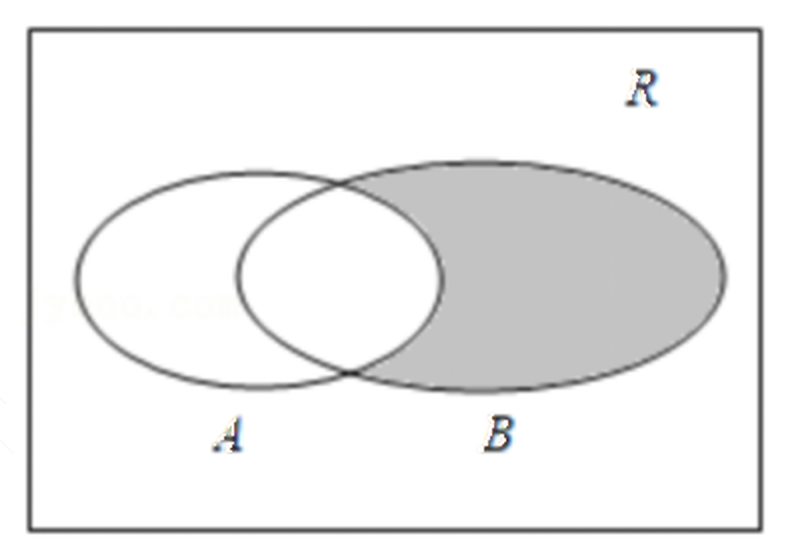
\includegraphics[width=0.36\textwidth]{figures/gao127_q4.png}
\end{center}

\ifanswer
\solbegin
\step{已知 $\R$ 是实数集，集合 $A=\{x\mid 1<x<2\}$, $B=\left\{x\mid 0<x<\frac32\right\}$,}
\step{阴影部分表示的集合是 $\overline A\cap B=\{x\mid 0<x\leqslant1\}$，即 $(0,1]$.}
\solend
\fi

\item 若集合 $\{x\mid (a-1)x^2+3x-2=0\}$ 有且仅有两个子集，则实数 $a$ 的值为\blankline[4.4em].

\ifanswer
\solbegin
\step{由题意得 $\{x\mid (a-1)x^2+3x-2=0\}$ 为单元素集，}
\step{所以 $a-1=0$ 或 $\begin{cases}a-1\neq0\\\triangle=9+8(a-1)=0\end{cases}$，所以 $a=1$ 或 $a=-\frac18$.}
\solend
\fi

\item 已知条件 $\alpha:x\leqslant m$，条件 $\beta:x^2-x\leqslant0$，若 $\alpha$ 是 $\beta$ 的必要条件，则实数 $m$ 的取值范围是为\blankline[4.4em].

\ifanswer
\solbegin
\step{不等式 $x^2-x\leqslant0$ 的解集为 $[0,1]$，}
\step{因为条件 $\alpha:x\leqslant m$，条件 $\beta:x^2-x\leqslant0$，且 $\alpha$ 是 $\beta$ 的必要条件，}
\step{所以集合 $[0,1]$ 是集合 $(-\infty,m]$ 的子集，得 $m\geqslant1$，实数 $m$ 的取值范围是 $[1,+\infty)$.}
\solend
\fi

\item 已知 $\alpha\in\{-2,-1,-\frac12,0,1,2\}$，若幂函数 $y=x^\alpha$ 在 $(0,+\infty)$ 是严格减函数且图像关于 $y$ 轴对称，则 $\alpha=$\blankline[4.4em].

\ifanswer
\solbegin
\step{幂函数 $y=x^\alpha$ 在 $(0,+\infty)$ 是严格减函数，则 $\alpha<0$，且图像关于 $y$ 轴对称，}
\step{则函数为偶函数，故 $\alpha=-2$.}
\solend
\fi

\item 若关于 $x$ 的不等式 $ax^2-3x+2<0$ 的解集不是空集，则实数 $a$ 的取值范围是\blankline[4.4em].

\ifanswer
\solbegin
\step{若 $a>0$，关于 $x$ 的不等式 $ax^2-3x+2<0$ 的解集不空，}
\step{所以一元二次方程 $ax^2-3x+2=0$ 的判别式大于零，}
\step{即 $(-3)^2-8a>0\Rightarrow a<\frac98$，结合 $a>0$ 得 $0<a<\frac98$；}
\step{若 $a\leqslant0$，则关于 $x$ 的不等式 $ax^2-3x+2<0$ 的解集不是空集；}
\step{综上，实数 $a$ 的取值范围是 $\left(-\infty,\frac98\right)$.}
\solend
\fi

\item 设 $\log_{18}2=a$，则 $\log_2 3$ 可用 $a$ 表示为\blankline[4.4em].

\ifanswer
\solbegin
\step{因为 $\log_{18}2=\frac{\log_2 2}{\log_2 18}=\frac1{1+2\log_2 3}=a$，则 $\log_2 3=\frac{1-a}{2a}$.}
\solend
\fi

\item 若关于 $x$ 的不等式 $ax^2+bx+c>0$ 解集为 $\left(-\frac12,3\right)$，则关于 $x$ 的不等式 $cx^2+bx+a<0$ 的解集为\blankline[4.4em].

\ifanswer
\solbegin
\step{由已知得 $a<0$，且 $ax^2+bx+c=a\left(x+\frac12\right)(x-3)$，}
\step{所以 $b=-\frac52 a, c=-\frac32 a$，}
\step{$cx^2+bx+a=-\frac a2(3x-1)(x+2)<0\Leftrightarrow(3x-1)(x+2)<0\Leftrightarrow -2<x<\frac13$，}
\step{故解集为 $\left(-2,\frac13\right)$.}
\solend
\fi

\item 设 $x\in\R$，则方程 $\lvert 2x+3\rvert-\lvert x-2\rvert=\lvert 3x+1\rvert$ 的解集为\blankline[4.4em].

\ifanswer
\solbegin
\step{当 $x\leqslant-\frac32$ 时，原式 $\Leftrightarrow -2x-3+x-2=-3x-1\Leftrightarrow x=2$，不合题意；}
\step{当 $-\frac32<x\leqslant-\frac13$ 时，原式 $\Leftrightarrow 2x+3+x-2=-3x-1\Leftrightarrow x=-\frac13$；}
\step{当 $-\frac13<x\leqslant2$ 时，原式 $\Leftrightarrow 2x+3+x-2=3x+1\Leftrightarrow 1=1$ 即恒成立；}
\step{当 $x>2$ 时，原式 $\Leftrightarrow 2x+3+2-x=3x+1\Leftrightarrow x=2$，不合题意；}
\step{故 $x\in\left[-\frac13,2\right]$.}
\solend
\fi

\item 若关于 $x$ 的不等式 $x^2-4mx+m<0$ 的解集为 $(x_1,x_2)$，若 $x_1>0,x_2>0$，试探究 $x_1+x_2,x_1x_2,x_1^2+x_2^2,\frac1{x_1}+\frac1{x_2}$ 的值，则 $4x_1+x_2$ 的最小值为\blankline[4.4em].

\ifanswer
\solbegin
\step{由题意得方程 $x^2-4mx+m=0$ 有两个相异的正实根 $x_1,x_2$，}
\step{故有 $\begin{cases}\triangle=16m^2-4m>0\\x_1+x_2=4m>0\\x_1\cdot x_2=m>0\end{cases}$，解得 $m>\frac14$，}
\step{则 $x_1^2+x_2^2=(x_1+x_2)^2-2x_1\cdot x_2=16m^2-2m$，$\frac1{x_1}+\frac1{x_2}=\frac{x_1+x_2}{x_1\cdot x_2}=4$，}
\step{则 $4x_1+x_2=\frac14(4x_1+x_2)\left(\frac1{x_1}+\frac1{x_2}\right)=\frac14\left(5+\frac{4x_1}{x_2}+\frac{x_2}{x_1}\right)\geqslant\frac94$，}
\step{当且仅当 $\frac{4x_1}{x_2}=\frac{x_2}{x_1}$ 时，即 $x_2=2x_1$ 时取等号，}
\step{由 $\begin{cases}x_2=2x_1\\\frac1{x_1}+\frac1{x_2}=4\end{cases}$，解得 $\begin{cases}x_1=\frac38\\x_2=\frac34\end{cases}$，于是 $m=x_1\cdot x_2=\frac9{32}\in\left(\frac14,+\infty\right)$，}
\step{即当 $m=\frac9{32}$ 时，$4x_1+x_2$ 取得最小值为 $\frac94$.}
\solend
\fi

\end{enumerate}

\bigsec{二、选择题}

\begin{enumerate}
\setcounter{enumi}{12}

\item 若 $a>0$, $a\neq1$, $M>0$, $N>0$，下列运算正确的是\mbox{（\quad）}

\keepwithprev
A. $\log_a\sqrt[N]{M}=\frac1N\log_a M$\qquad\qquad B. $(\log_a M)^N=N\log_a M$

C. $(\log_a M)\div(\log_a N)=\log_a(M-N)$\qquad\quad D. $\log_a M+\log_a N=\log_a(M+N)$

\ifanswer
\solbegin
\step{对于 $A$，$\log_a\sqrt[N]{M}=\log_a M^{\frac1N}=\frac1N\log_a M$，故 $A$ 正确；}
\step{对于 $B$，$(\log_a M)^N\neq N\log_a M=log_a M^n$，故 $B$ 错误；}
\step{对于 $C$，$(\log_a M)\div(\log_a N)\neq\log_a(M-N)$，故 $C$ 错误；}
\step{对于 $D$，$\log_a M+\log_a N=\log_a MN\neq\log_a(M+N)$，故 $D$ 错误.}
\step{故选 $A$.}
\solend
\fi

\item 下列不等式中正确的是\mbox{（\quad）}

\keepwithprev
A. 若 $a>b$，则 $ac^2>bc^2$\qquad\qquad B. 若 $a<b<0$，则 $a^2<b^2$

C. 若 $1<a<2$ 且 $0<b<3$，则 $1<a+b<5$\qquad D. 若 $\frac1a<1$，则 $a>1$

\ifanswer
\solbegin
\step{$C$ 中 $1+0<a+b<2+3$，即 $1<a+b<5$，正确.}
\step{$A$ 取 $c=0$ 时不成立；$B$ 应为 $a^2>b^2$；$D$ 取 $a=-1$ 时不成立. 故选 $C$.}
\solend
\fi

\item 已知 $y_1=x^3,y_2=x^2$，则下列说法正确的是\mbox{（\quad）}

\keepwithprev
A. $x\in(0,+\infty)$ 时，恒有 $y_1\geqslant y_2$

B. $y_1=x^3$ 与 $y_2=x^2$ 的函数图象仅有唯一交点

C. $x\in(0,1)$ 时，$y_1=x^3$ 图象在 $y_2=x^2$ 图象下方

D. 存在 $x_0\in(1,+\infty)$ 使得 $y_1=y_2$

\ifanswer
\solbegin
\step{$y_1-y_2=x^2(x-1)$，当 $0<x<1$ 时，$y_1<y_2$，故 $C$ 正确，$A$ 错误.}
\step{$y_1=y_2\Leftrightarrow x^2(x-1)=0\Leftrightarrow x=0$ 或 $x=1$，两图象有两个交点，故 $BD$ 错误.}
\step{故选 $C$.}
\solend
\fi

\item 已知非空集合 $A$、$B$ 满足两个条件：(1) $A\cup B=\{1,2,3,4,5,6,7\}$, $A\cap B=\varnothing$；(2) 若 $x\in A$，则 $x+1\in B$，则有序集合对 $(A,B)$ 的个数为\mbox{（\quad）}

\keepwithprev
A. $17$\qquad\qquad B. $18$\qquad\qquad C. $19$\qquad\qquad D. $20$

\ifanswer
\solbegin
\step{当 $A$ 为单元素集合时，有 6 种情况：}
\step{当 $A$ 为双元素集合时，$A=\{1,3\}, A=\{1,4\}, A=\{1,5\}, A=\{1,6\}, A=\{2,4\}$,}
\step{$A=\{2,5\}, A=\{2,6\}, A=\{3,5\}, A=\{3,6\}, A=\{4,6\}$，共 10 种情况；}
\step{当 $A$ 为三元素集合时，$A=\{1,3,5\}, A=\{1,3,6\}, A=\{1,4,6\}, A=\{2,4,6\}$，}
\step{共 4 种情况；}
\step{当 $A$ 为四元素集合时，不成立；}
\step{故有序集合对 $(A,B)$ 的个数为 20，故选 $D$.}
\solend
\fi

\end{enumerate}

\bigsec{三、解答题}

\begin{enumerate}
\setcounter{enumi}{16}

\item 已知 $x,y\in\R$，比较 $x^2+y^2$ 与 $2(2x-y)-5$ 的大小.

\ifanswer
\solbegin
\step{因为 $x^2+y^2-2(2x-y)+5=(x-2)^2+(y+1)^2\geqslant0$，}
\step{所以 $x^2+y^2\geqslant2(2x-y)-5$.}
\solend
\fi

\item 已知集合 $A=\{x\mid x^2+4x=0\}$，$B=\{x\mid x^2+2(a+1)x+a^2-1=0\}$.

(1) 若 $A$ 是 $B$ 的子集，求实数 $a$ 的值；

(2) 若 $B$ 是 $A$ 的子集，求实数 $a$ 的取值范围.

\ifanswer
\solbegin
\step{(1) 因为 $A=\{-4,0\}$，$B=\{x\mid x^2+2(a+1)x+a^2-1=0\}$，又 $A\subseteq B$，}
\step{所以 $A=B$，所以 $\begin{cases}-4+0=-2(a+1)\\-4\times0=a^2-1\end{cases}$，所以 $a=1$；}
\step{(2) 因为 $B$ 是 $A$ 的子集，所以 $B=\varnothing$ 或 $B=\{-4\}$ 或 $B=\{0\}$ 或 $B=\{-4,0\}$，}
\step{① $B=\varnothing$ 时，$\triangle=4(a+1)^2-4(a^2-1)<0$，所以 $a<-1$；}
\step{② $B=\{-4\}$ 时，$\begin{cases}-4+(-4)=-2(a+1)\\-4\times(-4)=a^2-1\end{cases}$，无解；}
\step{③ $B=\{0\}$ 时，$\begin{cases}0+0=-2(a+1)\\0\times0=a^2-1\end{cases}$，所以 $a=-1$；}
\step{④ $B=\{-4,0\}$ 时，由 (1) 得 $a=1$，}
\step{综上，实数 $a$ 的取值范围为 $(-\infty,-1]\cup\{1\}$.}
\solend
\fi

\item 某企业在现有设备下每日生产原先成本 $y$（单位：万元）与日产量 $x$（单位：吨）之间的函数关系式：$y=2x^2+(15-4k)x+120k+8$，近年来各部门都非常重视大气污染防治工作，为了配合环境卫生综合整治，该企业引进了除尘设备，每吨产品的除尘费用为 $k$ 万元，引进除尘设备后，当日产量 $x=1$ 时，总成本（总成本为原先成本和除尘费用之和）为 142 万元.

(1) 求 $k$ 的值；

(2) 求引进除尘设备后日产量为多少时，每吨产品的成本最小，并求出最小值.

\ifanswer
\solbegin
\step{(1) 该企业引进了除尘设备，}
\step{每日生产总成本 $h$（单位：万元）与日产量 $x$（单位：吨）之间的关系为}
\step{$h=2x^2+(15-4k)x+120k+8+kx=2x^2+(15-3k)x+120k+8$，}
\step{当日产量 $x=1$ 时，总成本为 $h=142$ 万元，}
\step{代入得 $2+(15-3k)+120k+8=142\Rightarrow k=1$，}
\step{(2) 由 (1) 得 $h=2x^2+12x+128$，}
\step{所以每吨产品的成本为 $w=\frac{2x^2+12x+128}{x}=2x+\frac{128}{x}+12$}
\step{$\geqslant2\sqrt{2x\cdot\frac{128}{x}}+12=44$，当且仅当 $2x=\frac{128}{x}$，即 $x=8$ 时，取等号，}
\step{所以引进除尘设备后日产量为 8 吨时，每吨产品的成本最小，}
\step{且最小值为 44 万元.}
\solend
\fi

\item 已知集合 $A=\{x\mid \lvert x-a\rvert<2\}$，集合 $B=\left\{x\mid\frac{2x-1}{x+2}<1\right\}$.

(1) 若 $a=2$，求 $A\cup B$；

(2) 若 $A\cap B=A$，求实数 $a$ 的取值范围.

\ifanswer
\solbegin
\step{(1) 若 $a=2$，则 $A=\{x\mid \lvert x-a\rvert<2\}=\{x\mid \lvert x-2\rvert<2\}=\{x\mid 0<x<4\}$，}
\step{由 $\frac{2x-1}{x+2}<1$ 得 $\frac{x-3}{x+2}<0$，即 $(x-3)(x+2)<0$，解得 $-2<x<3$，}
\step{所以 $B=\{x\mid -2<x<3\}$，所以 $A\cup B=\{x\mid -2<x<4\}$；}
\step{(2) 由 (1) 得 $B=\{x\mid -2<x<3\}$，}
\step{$A=\{x\mid \lvert x-a\rvert<2\}=\{x\mid a-2<x<a+2\}$，}
\step{若 $A\cap B=A$，则 $A\subseteq B$，则 $\begin{cases}a-2\geqslant-2\\a+2\leqslant3\end{cases}$，解得 $0\leqslant a\leqslant1$，}
\step{即实数 $a$ 的取值范围为 $[0,1]$.}
\solend
\fi

\item 已知自变量为 $x$ 的函数 $y=\frac{ax+b}{x+a}$，

(1) 若 $a=1$ 且 $b=2$，则函数 $y=\frac{ax+b}{x+a}$ 图像可由幂函数\blankline[4.4em]（写解析式）先沿 $x$ 轴方向\blankline[4.4em]平移\blankline[4.4em]个单位，再沿 $y$ 轴方向向上平移\blankline[4.4em]个单位得到；

(2) 当 $a>0$ 且 $b=-2$ 时不等式 $\frac{ax+b}{x+a}\leqslant\frac{2x^2}{x+a}$ 对 $x>0$ 恒成立，求实数 $a$ 的最大值；

(3) 若 $b=-2$ 且关于 $x$ 的不等式 $x^2\log_2\frac{4(a+1)}a+2x\log_2\frac{2a}{a+1}+\log_2\frac{(a+1)^2}{4a^2}\leqslant0$ 解集是单元素集，求出 $a$ 值，并求出函数 $y=\frac{ax-2}{x+a}$ 的对称中心.

\ifanswer
\solbegin
\step{(1) 已知自变量为 $x$ 的函数 $y=\frac{ax+b}{x+a}$，}
\step{当 $a=1$ 且 $b=2$ 时，$y=\frac{x+2}{x+1}=\frac{x+1+1}{x+1}=1+\frac1{x+1}$，}
\step{由幂函数 $y=\frac1x$，先沿 $x$ 轴方向向左平移一个单位，}
\step{再沿 $y$ 轴方向向上平移一个单位得到；}
\step{(2) 当 $a>0$ 且 $b=-2$ 时不等式 $\frac{ax+b}{x+a}\leqslant\frac{2x^2}{x+a}$ 即 $\frac{ax-2}{x+a}\leqslant\frac{2x^2}{x+a}$ 对 $x>0$ 恒成立，}
\step{因为 $a>0$ 且 $x>0$，所以 $x+a>0$，所以等价于 $ax-2\leqslant2x^2$ 对 $x>0$ 恒成立，}
\step{即 $2x^2-ax+2\geqslant0$ 对 $x>0$ 恒成立，}
\step{因为函数 $g(x)=2x^2-ax+2$ 的对称轴 $x=\frac a4>0$，且 $g(0)=2>0$，}
\step{则 $\begin{cases}\triangle=(-a)^2-4\times2\times2\leqslant0\\a>0\end{cases}$，解得 $0<a\leqslant4$，所以 $a$ 的最大值为 4；}
\step{(3) 关于 $x$ 的不等式 $x^2\log_2\frac{4(a+1)}a+2x\log_2\frac{2a}{a+1}+\log_2\frac{(a+1)^2}{4a^2}\leqslant0$ 解集}
\step{是单元素集，由 $\frac{4(a+1)}a>0$，则 $a>0$ 或 $a<-1$，}
\step{若 $\log_2\frac{4(a+1)}a=0$，则 $\frac{4(a+1)}a=1$，解得 $a=-\frac43$，}
\step{此时不等式为 $6x-6\leqslant0$，解得 $x\leqslant1$，不符合题意，}
\step{若 $\log_2\frac{4(a+1)}a>0$，即 $\frac{4(a+1)}a>1$，解得 $a>0$ 或 $a<-\frac43$，}
\step{则 $\triangle=\left(2\log_2\frac{2a}{a+1}\right)^2-4\log_2\frac{4(a+1)}a\cdot\log_2\frac{(a+1)^2}{4a^2}=0$，}
\step{令 $\log_2\frac{2a}{a+1}=t$，则 $t^2-(3-t)(-2t)=0$，解得 $t=0$ 或 $t=6$，}
\step{当 $\log_2\frac{2a}{a+1}=0$，解得 $a=1$，$\log_2\frac{2a}{a+1}=6$，解得 $a=-\frac{32}{31}$(舍去)，所以 $a=1$，}
\step{则函数 $y=\frac{ax-2}{x+a}$ 即为 $y=\frac{x-2}{x+1}=\frac{x+1-3}{x+1}=1+\frac{-3}{x+1}$，}
\step{对称中心为 $(-1,1)$.}
\solend
\fi

\end{enumerate}

\end{document}
"
%
% 原始材料：微信公众号“魔都数学加油站”文章，作者破晓，2026-11-11 18:35 发布；
% 连载“27学年高一127”，原文标题“27学年高一127——2026-2027年上海市南汇一中高一上期中”；
% 原文链接：https://mp.weixin.qq.com/s/nozIwRgeWSKPCPSiqfCm2Q。
% 正文为 9 张 PNG 页（01、02、03、09 为 2560×3620，04、05、06、07、08 为 4762×6735），
% 题目下印有【解析】，为讲评版。题目、解析均据原图转录；
% 卷面粉红色水印“魔都数学加油站”及公众号页脚未录入。全卷仅第 4 题一幅插图。
% 第 09 页只有一行“对称中心为(-1,1).”及水印，是第 08 页末行的续尾页。
%
% 卷首标题：原卷印作“2026-2027 年南汇一中高一上期中”（公众号标题中的“上海市”
% 卷面标题行没有，本稿照卷面），年份区间按全稿惯例排 en dash；原卷未印副标题，
% 本卷为期中卷、跨三章，按题目内容标为“集合与常用逻辑用语、不等式、函数”
% （第 4/5/6/16/18/20 题为集合与常用逻辑用语，第 8/10/11/12/14/17 题为不等式，
% 第 3/7/9/13/15/19/21 题为函数；与 106、125 同为期中复习卷，口径相同）。
%
% 与原卷的排版差异：
%   ① 原文从第 3 题起，填空题编号为 3—12、选择题为 13—16、解答题为 17—21，本稿保留原题号；
%   ② 原卷每题下直接印【解析】，本稿按全稿惯例置于答案版；四道选择题答案均在解析末句
%      “故选 …”，括号内留空、不另提 \ans{}；全卷无只印【答案】或括号内答案的题；
%   ③ 原卷未印副标题，本稿按“知识模块”口径补出；
%   ④ 原卷填空横线按全稿惯例排为 \blankline[4.4em]；选择题括号排 \mbox{（\quad）}、
%      选项段前按惯例加 \keepwithprev；解答题不留作答区（原卷为讲评版，与 109—125 同）；
%      第 21 题 (1) 的四处填空横线亦排 \blankline[4.4em]；
%   ⑤ 原卷数集排斜体 $R$，按全稿惯例改 \R；绝对值排 \lvert…\rvert，集合描述竖线排 \mid；
%      补集记号照原卷上划线排 \overline{A}；不等号一律 \leqslant / \geqslant；
%   ⑥ 第 4 题插图原在题干右侧，本稿按全稿惯例移至题干之后居中排（取原卷截图、
%      去粉色水印后 2× LANCZOS 放大，存 figures/gao127_q4.png），三版都出；
%      并在该题 \item 前加 \needvspace{} 守卫，把题干与插图整块推走；
%   ⑦ 原卷子题编号 (1)(2)(3) 与括号按全稿惯例排；“（单位：万元）”“（写解析式）”
%      用全角括号，第 21 题 (3) 解析“(舍去)”用半角括号，均照录；
%   ⑧ 第 09 页仅一行“对称中心为(-1,1).”为第 08 页末行之续尾，本稿按原卷印刷行
%      另起一条 \step，置于答案版最后一题解析之末。
%
% 子集符号：第 18 题 (1) 解析 $A\subseteq B$、第 20 题 (2) 解析 $A\subseteq B$ 均印有
%   下划线，照录 \subseteq；全卷无 \subset。回原图放大逐处确认。
%
% 判别式字形：本卷 5 处判别式（第 5 题解析 cases 内 $\triangle=9+8(a-1)=0$、
%   第 12 题解析 cases 内 $\triangle=16m^2-4m>0$、第 18 题① $\triangle=4(a+1)^2-4(a^2-1)<0$、
%   第 21 题 (2) cases 内 $\triangle=(-a)^2-4\times2\times2\leqslant0$、
%   第 21 题 (3) $\triangle=\left(2\log_2\frac{2a}{a+1}\right)^2-\cdots=0$）均排等边扁三角，
%   照录 \triangle；逐处回原图全分辨率放大确认，无高三角 $\Delta$（与 高一26 排 $\Delta$ 不同）。
%
% 原卷存疑照录：
%   第 6 题题干作“则实数 $m$ 的取值范围是为____”（“是为”叠用，疑衍一字），照录；
%   第 12 题题干“试探究 $x_1+x_2, x_1x_2, x_1^2+x_2^2, \frac1{x_1}+\frac1{x_2}$ 的值，
%     则 $4x_1+x_2$ 的最小值为____”与后文衔接突兀，照录；
%   第 13 题解析 B 作“$(\log_a M)^N\neq N\log_a M=log_a M^n$”，后一 log 为斜体、
%     指数作小写 $n$，与前式 $N\log_a M$ 及题干 $N$ 不一致，照录；
%   第 13 题解析 A、B、C 三步句末用“；”，D 步句末用“.”，标点不一致，照录；
%   第 15 题解析“故 $BD$ 错误.”两选项字母连写、无顿号，照录；
%   第 7 题题干及解析用“图像”，第 15 题 B、C 及解析用“图象”，全卷两种写法混用，照录未统一；
%   第 21 题 (3) 题干“求出 $a$ 值”（通常作“求出 $a$ 的值”），照录；
%   第 21 题 (3) 解析“解得 $a=1$，$\log_2\frac{2a}{a+1}=6$，解得 $a=-\frac{32}{31}$(舍去)，
%     所以 $a=1$”两个“解得”并列、且舍去值用半角括号，照录；
%   第 09 页“对称中心为(-1,1).”用半角括号与半角句点，照录；
%   第 8 题解析“若 $a\leqslant0$，则关于 $x$ 的不等式 $ax^2-3x+2<0$ 的解集不是空集；”
%     未给理由直接断言，照录；
%   第 18 题 (1) 由 $A\subseteq B$ 直接得 $A=B$，照录。
%
% 行数核对：逐题数 \step 条数，合计 95 条（Q3：1；Q4：2；Q5：2；Q6：3；Q7：2；
% Q8：5；Q9：1；Q10：4；Q11：5；Q12：7；Q13：5；Q14：2；Q15：3；Q16：7；
% Q17：2；Q18：8；Q19：10；Q20：7；Q21：19），与原卷印刷行逐题相等
% （cases 块作一个印刷行计；Q21 第 19 行为第 09 页续尾）。全卷 19 题均印【解析】，
% 无只印【答案】或括号内答案的题，故 \ans{} 为 0；四道选择题括号内留空、不另提 \ans{}。
%
\documentclass[a4paper,11pt]{article}
\usepackage{common}

\begin{document}

\examtitlest[3]{2026--2027 年南汇一中高一上期中}{集合与常用逻辑用语、不等式、函数}

\bigsec{一、填空题}

\begin{enumerate}
\setcounter{enumi}{2}

\item 把 $\sqrt[4]{a\sqrt a}(a>0)$ 化成有理数指数幂的形式为\blankline[4.4em].

\ifanswer
\solbegin
\step{$\sqrt[4]{a\sqrt a}=(a\cdot a^{\frac12})^{\frac14}=a^{\frac38}$.}
\solend
\fi

\needvspace{6.5cm}
\item 已知集合 $A=\{x\mid 1<x<2\}$, $B=\left\{x\mid 0<x<\frac32\right\}$, 则如图阴影部分表示的集合是\blankline[4.4em].

\begin{center}
% 图取原卷截图（第 1 页题干右侧）、去水印后 2× LANCZOS 放大，本稿移至题干之后
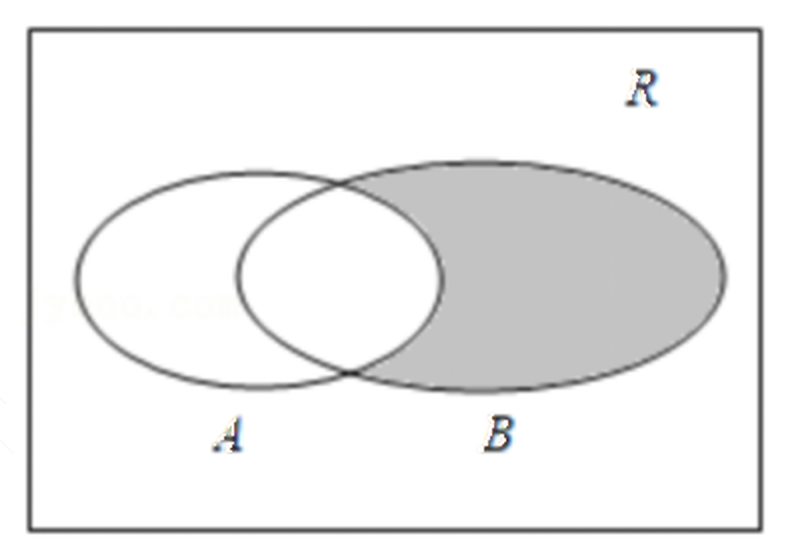
\includegraphics[width=0.36\textwidth]{figures/gao127_q4.png}
\end{center}

\ifanswer
\solbegin
\step{已知 $\R$ 是实数集，集合 $A=\{x\mid 1<x<2\}$, $B=\left\{x\mid 0<x<\frac32\right\}$,}
\step{阴影部分表示的集合是 $\overline A\cap B=\{x\mid 0<x\leqslant1\}$，即 $(0,1]$.}
\solend
\fi

\item 若集合 $\{x\mid (a-1)x^2+3x-2=0\}$ 有且仅有两个子集，则实数 $a$ 的值为\blankline[4.4em].

\ifanswer
\solbegin
\step{由题意得 $\{x\mid (a-1)x^2+3x-2=0\}$ 为单元素集，}
\step{所以 $a-1=0$ 或 $\begin{cases}a-1\neq0\\\triangle=9+8(a-1)=0\end{cases}$，所以 $a=1$ 或 $a=-\frac18$.}
\solend
\fi

\item 已知条件 $\alpha:x\leqslant m$，条件 $\beta:x^2-x\leqslant0$，若 $\alpha$ 是 $\beta$ 的必要条件，则实数 $m$ 的取值范围是为\blankline[4.4em].

\ifanswer
\solbegin
\step{不等式 $x^2-x\leqslant0$ 的解集为 $[0,1]$，}
\step{因为条件 $\alpha:x\leqslant m$，条件 $\beta:x^2-x\leqslant0$，且 $\alpha$ 是 $\beta$ 的必要条件，}
\step{所以集合 $[0,1]$ 是集合 $(-\infty,m]$ 的子集，得 $m\geqslant1$，实数 $m$ 的取值范围是 $[1,+\infty)$.}
\solend
\fi

\item 已知 $\alpha\in\{-2,-1,-\frac12,0,1,2\}$，若幂函数 $y=x^\alpha$ 在 $(0,+\infty)$ 是严格减函数且图像关于 $y$ 轴对称，则 $\alpha=$\blankline[4.4em].

\ifanswer
\solbegin
\step{幂函数 $y=x^\alpha$ 在 $(0,+\infty)$ 是严格减函数，则 $\alpha<0$，且图像关于 $y$ 轴对称，}
\step{则函数为偶函数，故 $\alpha=-2$.}
\solend
\fi

\item 若关于 $x$ 的不等式 $ax^2-3x+2<0$ 的解集不是空集，则实数 $a$ 的取值范围是\blankline[4.4em].

\ifanswer
\solbegin
\step{若 $a>0$，关于 $x$ 的不等式 $ax^2-3x+2<0$ 的解集不空，}
\step{所以一元二次方程 $ax^2-3x+2=0$ 的判别式大于零，}
\step{即 $(-3)^2-8a>0\Rightarrow a<\frac98$，结合 $a>0$ 得 $0<a<\frac98$；}
\step{若 $a\leqslant0$，则关于 $x$ 的不等式 $ax^2-3x+2<0$ 的解集不是空集；}
\step{综上，实数 $a$ 的取值范围是 $\left(-\infty,\frac98\right)$.}
\solend
\fi

\item 设 $\log_{18}2=a$，则 $\log_2 3$ 可用 $a$ 表示为\blankline[4.4em].

\ifanswer
\solbegin
\step{因为 $\log_{18}2=\frac{\log_2 2}{\log_2 18}=\frac1{1+2\log_2 3}=a$，则 $\log_2 3=\frac{1-a}{2a}$.}
\solend
\fi

\item 若关于 $x$ 的不等式 $ax^2+bx+c>0$ 解集为 $\left(-\frac12,3\right)$，则关于 $x$ 的不等式 $cx^2+bx+a<0$ 的解集为\blankline[4.4em].

\ifanswer
\solbegin
\step{由已知得 $a<0$，且 $ax^2+bx+c=a\left(x+\frac12\right)(x-3)$，}
\step{所以 $b=-\frac52 a, c=-\frac32 a$，}
\step{$cx^2+bx+a=-\frac a2(3x-1)(x+2)<0\Leftrightarrow(3x-1)(x+2)<0\Leftrightarrow -2<x<\frac13$，}
\step{故解集为 $\left(-2,\frac13\right)$.}
\solend
\fi

\item 设 $x\in\R$，则方程 $\lvert 2x+3\rvert-\lvert x-2\rvert=\lvert 3x+1\rvert$ 的解集为\blankline[4.4em].

\ifanswer
\solbegin
\step{当 $x\leqslant-\frac32$ 时，原式 $\Leftrightarrow -2x-3+x-2=-3x-1\Leftrightarrow x=2$，不合题意；}
\step{当 $-\frac32<x\leqslant-\frac13$ 时，原式 $\Leftrightarrow 2x+3+x-2=-3x-1\Leftrightarrow x=-\frac13$；}
\step{当 $-\frac13<x\leqslant2$ 时，原式 $\Leftrightarrow 2x+3+x-2=3x+1\Leftrightarrow 1=1$ 即恒成立；}
\step{当 $x>2$ 时，原式 $\Leftrightarrow 2x+3+2-x=3x+1\Leftrightarrow x=2$，不合题意；}
\step{故 $x\in\left[-\frac13,2\right]$.}
\solend
\fi

\item 若关于 $x$ 的不等式 $x^2-4mx+m<0$ 的解集为 $(x_1,x_2)$，若 $x_1>0,x_2>0$，试探究 $x_1+x_2,x_1x_2,x_1^2+x_2^2,\frac1{x_1}+\frac1{x_2}$ 的值，则 $4x_1+x_2$ 的最小值为\blankline[4.4em].

\ifanswer
\solbegin
\step{由题意得方程 $x^2-4mx+m=0$ 有两个相异的正实根 $x_1,x_2$，}
\step{故有 $\begin{cases}\triangle=16m^2-4m>0\\x_1+x_2=4m>0\\x_1\cdot x_2=m>0\end{cases}$，解得 $m>\frac14$，}
\step{则 $x_1^2+x_2^2=(x_1+x_2)^2-2x_1\cdot x_2=16m^2-2m$，$\frac1{x_1}+\frac1{x_2}=\frac{x_1+x_2}{x_1\cdot x_2}=4$，}
\step{则 $4x_1+x_2=\frac14(4x_1+x_2)\left(\frac1{x_1}+\frac1{x_2}\right)=\frac14\left(5+\frac{4x_1}{x_2}+\frac{x_2}{x_1}\right)\geqslant\frac94$，}
\step{当且仅当 $\frac{4x_1}{x_2}=\frac{x_2}{x_1}$ 时，即 $x_2=2x_1$ 时取等号，}
\step{由 $\begin{cases}x_2=2x_1\\\frac1{x_1}+\frac1{x_2}=4\end{cases}$，解得 $\begin{cases}x_1=\frac38\\x_2=\frac34\end{cases}$，于是 $m=x_1\cdot x_2=\frac9{32}\in\left(\frac14,+\infty\right)$，}
\step{即当 $m=\frac9{32}$ 时，$4x_1+x_2$ 取得最小值为 $\frac94$.}
\solend
\fi

\end{enumerate}

\bigsec{二、选择题}

\begin{enumerate}
\setcounter{enumi}{12}

\item 若 $a>0$, $a\neq1$, $M>0$, $N>0$，下列运算正确的是\mbox{（\quad）}

\keepwithprev
A. $\log_a\sqrt[N]{M}=\frac1N\log_a M$\qquad\qquad B. $(\log_a M)^N=N\log_a M$

C. $(\log_a M)\div(\log_a N)=\log_a(M-N)$\qquad\quad D. $\log_a M+\log_a N=\log_a(M+N)$

\ifanswer
\solbegin
\step{对于 $A$，$\log_a\sqrt[N]{M}=\log_a M^{\frac1N}=\frac1N\log_a M$，故 $A$ 正确；}
\step{对于 $B$，$(\log_a M)^N\neq N\log_a M=log_a M^n$，故 $B$ 错误；}
\step{对于 $C$，$(\log_a M)\div(\log_a N)\neq\log_a(M-N)$，故 $C$ 错误；}
\step{对于 $D$，$\log_a M+\log_a N=\log_a MN\neq\log_a(M+N)$，故 $D$ 错误.}
\step{故选 $A$.}
\solend
\fi

\item 下列不等式中正确的是\mbox{（\quad）}

\keepwithprev
A. 若 $a>b$，则 $ac^2>bc^2$\qquad\qquad B. 若 $a<b<0$，则 $a^2<b^2$

C. 若 $1<a<2$ 且 $0<b<3$，则 $1<a+b<5$\qquad D. 若 $\frac1a<1$，则 $a>1$

\ifanswer
\solbegin
\step{$C$ 中 $1+0<a+b<2+3$，即 $1<a+b<5$，正确.}
\step{$A$ 取 $c=0$ 时不成立；$B$ 应为 $a^2>b^2$；$D$ 取 $a=-1$ 时不成立. 故选 $C$.}
\solend
\fi

\item 已知 $y_1=x^3,y_2=x^2$，则下列说法正确的是\mbox{（\quad）}

\keepwithprev
A. $x\in(0,+\infty)$ 时，恒有 $y_1\geqslant y_2$

B. $y_1=x^3$ 与 $y_2=x^2$ 的函数图象仅有唯一交点

C. $x\in(0,1)$ 时，$y_1=x^3$ 图象在 $y_2=x^2$ 图象下方

D. 存在 $x_0\in(1,+\infty)$ 使得 $y_1=y_2$

\ifanswer
\solbegin
\step{$y_1-y_2=x^2(x-1)$，当 $0<x<1$ 时，$y_1<y_2$，故 $C$ 正确，$A$ 错误.}
\step{$y_1=y_2\Leftrightarrow x^2(x-1)=0\Leftrightarrow x=0$ 或 $x=1$，两图象有两个交点，故 $BD$ 错误.}
\step{故选 $C$.}
\solend
\fi

\item 已知非空集合 $A$、$B$ 满足两个条件：(1) $A\cup B=\{1,2,3,4,5,6,7\}$, $A\cap B=\varnothing$；(2) 若 $x\in A$，则 $x+1\in B$，则有序集合对 $(A,B)$ 的个数为\mbox{（\quad）}

\keepwithprev
A. $17$\qquad\qquad B. $18$\qquad\qquad C. $19$\qquad\qquad D. $20$

\ifanswer
\solbegin
\step{当 $A$ 为单元素集合时，有 6 种情况：}
\step{当 $A$ 为双元素集合时，$A=\{1,3\}, A=\{1,4\}, A=\{1,5\}, A=\{1,6\}, A=\{2,4\}$,}
\step{$A=\{2,5\}, A=\{2,6\}, A=\{3,5\}, A=\{3,6\}, A=\{4,6\}$，共 10 种情况；}
\step{当 $A$ 为三元素集合时，$A=\{1,3,5\}, A=\{1,3,6\}, A=\{1,4,6\}, A=\{2,4,6\}$，}
\step{共 4 种情况；}
\step{当 $A$ 为四元素集合时，不成立；}
\step{故有序集合对 $(A,B)$ 的个数为 20，故选 $D$.}
\solend
\fi

\end{enumerate}

\bigsec{三、解答题}

\begin{enumerate}
\setcounter{enumi}{16}

\item 已知 $x,y\in\R$，比较 $x^2+y^2$ 与 $2(2x-y)-5$ 的大小.

\ifanswer
\solbegin
\step{因为 $x^2+y^2-2(2x-y)+5=(x-2)^2+(y+1)^2\geqslant0$，}
\step{所以 $x^2+y^2\geqslant2(2x-y)-5$.}
\solend
\fi

\item 已知集合 $A=\{x\mid x^2+4x=0\}$，$B=\{x\mid x^2+2(a+1)x+a^2-1=0\}$.

(1) 若 $A$ 是 $B$ 的子集，求实数 $a$ 的值；

(2) 若 $B$ 是 $A$ 的子集，求实数 $a$ 的取值范围.

\ifanswer
\solbegin
\step{(1) 因为 $A=\{-4,0\}$，$B=\{x\mid x^2+2(a+1)x+a^2-1=0\}$，又 $A\subseteq B$，}
\step{所以 $A=B$，所以 $\begin{cases}-4+0=-2(a+1)\\-4\times0=a^2-1\end{cases}$，所以 $a=1$；}
\step{(2) 因为 $B$ 是 $A$ 的子集，所以 $B=\varnothing$ 或 $B=\{-4\}$ 或 $B=\{0\}$ 或 $B=\{-4,0\}$，}
\step{① $B=\varnothing$ 时，$\triangle=4(a+1)^2-4(a^2-1)<0$，所以 $a<-1$；}
\step{② $B=\{-4\}$ 时，$\begin{cases}-4+(-4)=-2(a+1)\\-4\times(-4)=a^2-1\end{cases}$，无解；}
\step{③ $B=\{0\}$ 时，$\begin{cases}0+0=-2(a+1)\\0\times0=a^2-1\end{cases}$，所以 $a=-1$；}
\step{④ $B=\{-4,0\}$ 时，由 (1) 得 $a=1$，}
\step{综上，实数 $a$ 的取值范围为 $(-\infty,-1]\cup\{1\}$.}
\solend
\fi

\item 某企业在现有设备下每日生产原先成本 $y$（单位：万元）与日产量 $x$（单位：吨）之间的函数关系式：$y=2x^2+(15-4k)x+120k+8$，近年来各部门都非常重视大气污染防治工作，为了配合环境卫生综合整治，该企业引进了除尘设备，每吨产品的除尘费用为 $k$ 万元，引进除尘设备后，当日产量 $x=1$ 时，总成本（总成本为原先成本和除尘费用之和）为 142 万元.

(1) 求 $k$ 的值；

(2) 求引进除尘设备后日产量为多少时，每吨产品的成本最小，并求出最小值.

\ifanswer
\solbegin
\step{(1) 该企业引进了除尘设备，}
\step{每日生产总成本 $h$（单位：万元）与日产量 $x$（单位：吨）之间的关系为}
\step{$h=2x^2+(15-4k)x+120k+8+kx=2x^2+(15-3k)x+120k+8$，}
\step{当日产量 $x=1$ 时，总成本为 $h=142$ 万元，}
\step{代入得 $2+(15-3k)+120k+8=142\Rightarrow k=1$，}
\step{(2) 由 (1) 得 $h=2x^2+12x+128$，}
\step{所以每吨产品的成本为 $w=\frac{2x^2+12x+128}{x}=2x+\frac{128}{x}+12$}
\step{$\geqslant2\sqrt{2x\cdot\frac{128}{x}}+12=44$，当且仅当 $2x=\frac{128}{x}$，即 $x=8$ 时，取等号，}
\step{所以引进除尘设备后日产量为 8 吨时，每吨产品的成本最小，}
\step{且最小值为 44 万元.}
\solend
\fi

\item 已知集合 $A=\{x\mid \lvert x-a\rvert<2\}$，集合 $B=\left\{x\mid\frac{2x-1}{x+2}<1\right\}$.

(1) 若 $a=2$，求 $A\cup B$；

(2) 若 $A\cap B=A$，求实数 $a$ 的取值范围.

\ifanswer
\solbegin
\step{(1) 若 $a=2$，则 $A=\{x\mid \lvert x-a\rvert<2\}=\{x\mid \lvert x-2\rvert<2\}=\{x\mid 0<x<4\}$，}
\step{由 $\frac{2x-1}{x+2}<1$ 得 $\frac{x-3}{x+2}<0$，即 $(x-3)(x+2)<0$，解得 $-2<x<3$，}
\step{所以 $B=\{x\mid -2<x<3\}$，所以 $A\cup B=\{x\mid -2<x<4\}$；}
\step{(2) 由 (1) 得 $B=\{x\mid -2<x<3\}$，}
\step{$A=\{x\mid \lvert x-a\rvert<2\}=\{x\mid a-2<x<a+2\}$，}
\step{若 $A\cap B=A$，则 $A\subseteq B$，则 $\begin{cases}a-2\geqslant-2\\a+2\leqslant3\end{cases}$，解得 $0\leqslant a\leqslant1$，}
\step{即实数 $a$ 的取值范围为 $[0,1]$.}
\solend
\fi

\item 已知自变量为 $x$ 的函数 $y=\frac{ax+b}{x+a}$，

(1) 若 $a=1$ 且 $b=2$，则函数 $y=\frac{ax+b}{x+a}$ 图像可由幂函数\blankline[4.4em]（写解析式）先沿 $x$ 轴方向\blankline[4.4em]平移\blankline[4.4em]个单位，再沿 $y$ 轴方向向上平移\blankline[4.4em]个单位得到；

(2) 当 $a>0$ 且 $b=-2$ 时不等式 $\frac{ax+b}{x+a}\leqslant\frac{2x^2}{x+a}$ 对 $x>0$ 恒成立，求实数 $a$ 的最大值；

(3) 若 $b=-2$ 且关于 $x$ 的不等式 $x^2\log_2\frac{4(a+1)}a+2x\log_2\frac{2a}{a+1}+\log_2\frac{(a+1)^2}{4a^2}\leqslant0$ 解集是单元素集，求出 $a$ 值，并求出函数 $y=\frac{ax-2}{x+a}$ 的对称中心.

\ifanswer
\solbegin
\step{(1) 已知自变量为 $x$ 的函数 $y=\frac{ax+b}{x+a}$，}
\step{当 $a=1$ 且 $b=2$ 时，$y=\frac{x+2}{x+1}=\frac{x+1+1}{x+1}=1+\frac1{x+1}$，}
\step{由幂函数 $y=\frac1x$，先沿 $x$ 轴方向向左平移一个单位，}
\step{再沿 $y$ 轴方向向上平移一个单位得到；}
\step{(2) 当 $a>0$ 且 $b=-2$ 时不等式 $\frac{ax+b}{x+a}\leqslant\frac{2x^2}{x+a}$ 即 $\frac{ax-2}{x+a}\leqslant\frac{2x^2}{x+a}$ 对 $x>0$ 恒成立，}
\step{因为 $a>0$ 且 $x>0$，所以 $x+a>0$，所以等价于 $ax-2\leqslant2x^2$ 对 $x>0$ 恒成立，}
\step{即 $2x^2-ax+2\geqslant0$ 对 $x>0$ 恒成立，}
\step{因为函数 $g(x)=2x^2-ax+2$ 的对称轴 $x=\frac a4>0$，且 $g(0)=2>0$，}
\step{则 $\begin{cases}\triangle=(-a)^2-4\times2\times2\leqslant0\\a>0\end{cases}$，解得 $0<a\leqslant4$，所以 $a$ 的最大值为 4；}
\step{(3) 关于 $x$ 的不等式 $x^2\log_2\frac{4(a+1)}a+2x\log_2\frac{2a}{a+1}+\log_2\frac{(a+1)^2}{4a^2}\leqslant0$ 解集}
\step{是单元素集，由 $\frac{4(a+1)}a>0$，则 $a>0$ 或 $a<-1$，}
\step{若 $\log_2\frac{4(a+1)}a=0$，则 $\frac{4(a+1)}a=1$，解得 $a=-\frac43$，}
\step{此时不等式为 $6x-6\leqslant0$，解得 $x\leqslant1$，不符合题意，}
\step{若 $\log_2\frac{4(a+1)}a>0$，即 $\frac{4(a+1)}a>1$，解得 $a>0$ 或 $a<-\frac43$，}
\step{则 $\triangle=\left(2\log_2\frac{2a}{a+1}\right)^2-4\log_2\frac{4(a+1)}a\cdot\log_2\frac{(a+1)^2}{4a^2}=0$，}
\step{令 $\log_2\frac{2a}{a+1}=t$，则 $t^2-(3-t)(-2t)=0$，解得 $t=0$ 或 $t=6$，}
\step{当 $\log_2\frac{2a}{a+1}=0$，解得 $a=1$，$\log_2\frac{2a}{a+1}=6$，解得 $a=-\frac{32}{31}$(舍去)，所以 $a=1$，}
\step{则函数 $y=\frac{ax-2}{x+a}$ 即为 $y=\frac{x-2}{x+1}=\frac{x+1-3}{x+1}=1+\frac{-3}{x+1}$，}
\step{对称中心为 $(-1,1)$.}
\solend
\fi

\end{enumerate}

\end{document}
"
% 紧凑版：xelatex "\def\iscompact{1}% 高一127_南汇一中_期中.tex
%   —— 高一上数学“2026-2027 年南汇一中高一上期中”（试卷版/答案版）
% 试卷版：xelatex 高一127_南汇一中_期中.tex
% 答案版：xelatex "\def\isanswer{1}% 高一127_南汇一中_期中.tex
%   —— 高一上数学“2026-2027 年南汇一中高一上期中”（试卷版/答案版）
% 试卷版：xelatex 高一127_南汇一中_期中.tex
% 答案版：xelatex "\def\isanswer{1}\input{高一127_南汇一中_期中.tex}"
% 紧凑版：xelatex "\def\iscompact{1}\input{高一127_南汇一中_期中.tex}"
%
% 原始材料：微信公众号“魔都数学加油站”文章，作者破晓，2026-11-11 18:35 发布；
% 连载“27学年高一127”，原文标题“27学年高一127——2026-2027年上海市南汇一中高一上期中”；
% 原文链接：https://mp.weixin.qq.com/s/nozIwRgeWSKPCPSiqfCm2Q。
% 正文为 9 张 PNG 页（01、02、03、09 为 2560×3620，04、05、06、07、08 为 4762×6735），
% 题目下印有【解析】，为讲评版。题目、解析均据原图转录；
% 卷面粉红色水印“魔都数学加油站”及公众号页脚未录入。全卷仅第 4 题一幅插图。
% 第 09 页只有一行“对称中心为(-1,1).”及水印，是第 08 页末行的续尾页。
%
% 卷首标题：原卷印作“2026-2027 年南汇一中高一上期中”（公众号标题中的“上海市”
% 卷面标题行没有，本稿照卷面），年份区间按全稿惯例排 en dash；原卷未印副标题，
% 本卷为期中卷、跨三章，按题目内容标为“集合与常用逻辑用语、不等式、函数”
% （第 4/5/6/16/18/20 题为集合与常用逻辑用语，第 8/10/11/12/14/17 题为不等式，
% 第 3/7/9/13/15/19/21 题为函数；与 106、125 同为期中复习卷，口径相同）。
%
% 与原卷的排版差异：
%   ① 原文从第 3 题起，填空题编号为 3—12、选择题为 13—16、解答题为 17—21，本稿保留原题号；
%   ② 原卷每题下直接印【解析】，本稿按全稿惯例置于答案版；四道选择题答案均在解析末句
%      “故选 …”，括号内留空、不另提 \ans{}；全卷无只印【答案】或括号内答案的题；
%   ③ 原卷未印副标题，本稿按“知识模块”口径补出；
%   ④ 原卷填空横线按全稿惯例排为 \blankline[4.4em]；选择题括号排 \mbox{（\quad）}、
%      选项段前按惯例加 \keepwithprev；解答题不留作答区（原卷为讲评版，与 109—125 同）；
%      第 21 题 (1) 的四处填空横线亦排 \blankline[4.4em]；
%   ⑤ 原卷数集排斜体 $R$，按全稿惯例改 \R；绝对值排 \lvert…\rvert，集合描述竖线排 \mid；
%      补集记号照原卷上划线排 \overline{A}；不等号一律 \leqslant / \geqslant；
%   ⑥ 第 4 题插图原在题干右侧，本稿按全稿惯例移至题干之后居中排（取原卷截图、
%      去粉色水印后 2× LANCZOS 放大，存 figures/gao127_q4.png），三版都出；
%      并在该题 \item 前加 \needvspace{} 守卫，把题干与插图整块推走；
%   ⑦ 原卷子题编号 (1)(2)(3) 与括号按全稿惯例排；“（单位：万元）”“（写解析式）”
%      用全角括号，第 21 题 (3) 解析“(舍去)”用半角括号，均照录；
%   ⑧ 第 09 页仅一行“对称中心为(-1,1).”为第 08 页末行之续尾，本稿按原卷印刷行
%      另起一条 \step，置于答案版最后一题解析之末。
%
% 子集符号：第 18 题 (1) 解析 $A\subseteq B$、第 20 题 (2) 解析 $A\subseteq B$ 均印有
%   下划线，照录 \subseteq；全卷无 \subset。回原图放大逐处确认。
%
% 判别式字形：本卷 5 处判别式（第 5 题解析 cases 内 $\triangle=9+8(a-1)=0$、
%   第 12 题解析 cases 内 $\triangle=16m^2-4m>0$、第 18 题① $\triangle=4(a+1)^2-4(a^2-1)<0$、
%   第 21 题 (2) cases 内 $\triangle=(-a)^2-4\times2\times2\leqslant0$、
%   第 21 题 (3) $\triangle=\left(2\log_2\frac{2a}{a+1}\right)^2-\cdots=0$）均排等边扁三角，
%   照录 \triangle；逐处回原图全分辨率放大确认，无高三角 $\Delta$（与 高一26 排 $\Delta$ 不同）。
%
% 原卷存疑照录：
%   第 6 题题干作“则实数 $m$ 的取值范围是为____”（“是为”叠用，疑衍一字），照录；
%   第 12 题题干“试探究 $x_1+x_2, x_1x_2, x_1^2+x_2^2, \frac1{x_1}+\frac1{x_2}$ 的值，
%     则 $4x_1+x_2$ 的最小值为____”与后文衔接突兀，照录；
%   第 13 题解析 B 作“$(\log_a M)^N\neq N\log_a M=log_a M^n$”，后一 log 为斜体、
%     指数作小写 $n$，与前式 $N\log_a M$ 及题干 $N$ 不一致，照录；
%   第 13 题解析 A、B、C 三步句末用“；”，D 步句末用“.”，标点不一致，照录；
%   第 15 题解析“故 $BD$ 错误.”两选项字母连写、无顿号，照录；
%   第 7 题题干及解析用“图像”，第 15 题 B、C 及解析用“图象”，全卷两种写法混用，照录未统一；
%   第 21 题 (3) 题干“求出 $a$ 值”（通常作“求出 $a$ 的值”），照录；
%   第 21 题 (3) 解析“解得 $a=1$，$\log_2\frac{2a}{a+1}=6$，解得 $a=-\frac{32}{31}$(舍去)，
%     所以 $a=1$”两个“解得”并列、且舍去值用半角括号，照录；
%   第 09 页“对称中心为(-1,1).”用半角括号与半角句点，照录；
%   第 8 题解析“若 $a\leqslant0$，则关于 $x$ 的不等式 $ax^2-3x+2<0$ 的解集不是空集；”
%     未给理由直接断言，照录；
%   第 18 题 (1) 由 $A\subseteq B$ 直接得 $A=B$，照录。
%
% 行数核对：逐题数 \step 条数，合计 95 条（Q3：1；Q4：2；Q5：2；Q6：3；Q7：2；
% Q8：5；Q9：1；Q10：4；Q11：5；Q12：7；Q13：5；Q14：2；Q15：3；Q16：7；
% Q17：2；Q18：8；Q19：10；Q20：7；Q21：19），与原卷印刷行逐题相等
% （cases 块作一个印刷行计；Q21 第 19 行为第 09 页续尾）。全卷 19 题均印【解析】，
% 无只印【答案】或括号内答案的题，故 \ans{} 为 0；四道选择题括号内留空、不另提 \ans{}。
%
\documentclass[a4paper,11pt]{article}
\usepackage{common}

\begin{document}

\examtitlest[3]{2026--2027 年南汇一中高一上期中}{集合与常用逻辑用语、不等式、函数}

\bigsec{一、填空题}

\begin{enumerate}
\setcounter{enumi}{2}

\item 把 $\sqrt[4]{a\sqrt a}(a>0)$ 化成有理数指数幂的形式为\blankline[4.4em].

\ifanswer
\solbegin
\step{$\sqrt[4]{a\sqrt a}=(a\cdot a^{\frac12})^{\frac14}=a^{\frac38}$.}
\solend
\fi

\needvspace{6.5cm}
\item 已知集合 $A=\{x\mid 1<x<2\}$, $B=\left\{x\mid 0<x<\frac32\right\}$, 则如图阴影部分表示的集合是\blankline[4.4em].

\begin{center}
% 图取原卷截图（第 1 页题干右侧）、去水印后 2× LANCZOS 放大，本稿移至题干之后
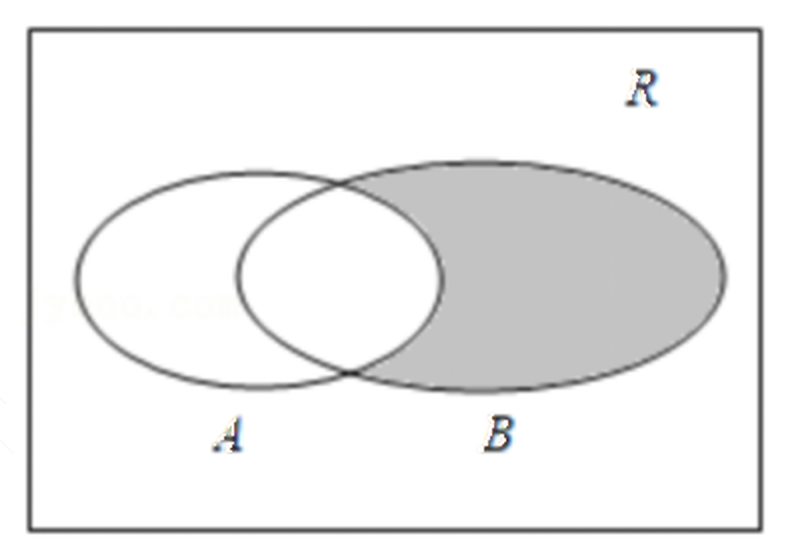
\includegraphics[width=0.36\textwidth]{figures/gao127_q4.png}
\end{center}

\ifanswer
\solbegin
\step{已知 $\R$ 是实数集，集合 $A=\{x\mid 1<x<2\}$, $B=\left\{x\mid 0<x<\frac32\right\}$,}
\step{阴影部分表示的集合是 $\overline A\cap B=\{x\mid 0<x\leqslant1\}$，即 $(0,1]$.}
\solend
\fi

\item 若集合 $\{x\mid (a-1)x^2+3x-2=0\}$ 有且仅有两个子集，则实数 $a$ 的值为\blankline[4.4em].

\ifanswer
\solbegin
\step{由题意得 $\{x\mid (a-1)x^2+3x-2=0\}$ 为单元素集，}
\step{所以 $a-1=0$ 或 $\begin{cases}a-1\neq0\\\triangle=9+8(a-1)=0\end{cases}$，所以 $a=1$ 或 $a=-\frac18$.}
\solend
\fi

\item 已知条件 $\alpha:x\leqslant m$，条件 $\beta:x^2-x\leqslant0$，若 $\alpha$ 是 $\beta$ 的必要条件，则实数 $m$ 的取值范围是为\blankline[4.4em].

\ifanswer
\solbegin
\step{不等式 $x^2-x\leqslant0$ 的解集为 $[0,1]$，}
\step{因为条件 $\alpha:x\leqslant m$，条件 $\beta:x^2-x\leqslant0$，且 $\alpha$ 是 $\beta$ 的必要条件，}
\step{所以集合 $[0,1]$ 是集合 $(-\infty,m]$ 的子集，得 $m\geqslant1$，实数 $m$ 的取值范围是 $[1,+\infty)$.}
\solend
\fi

\item 已知 $\alpha\in\{-2,-1,-\frac12,0,1,2\}$，若幂函数 $y=x^\alpha$ 在 $(0,+\infty)$ 是严格减函数且图像关于 $y$ 轴对称，则 $\alpha=$\blankline[4.4em].

\ifanswer
\solbegin
\step{幂函数 $y=x^\alpha$ 在 $(0,+\infty)$ 是严格减函数，则 $\alpha<0$，且图像关于 $y$ 轴对称，}
\step{则函数为偶函数，故 $\alpha=-2$.}
\solend
\fi

\item 若关于 $x$ 的不等式 $ax^2-3x+2<0$ 的解集不是空集，则实数 $a$ 的取值范围是\blankline[4.4em].

\ifanswer
\solbegin
\step{若 $a>0$，关于 $x$ 的不等式 $ax^2-3x+2<0$ 的解集不空，}
\step{所以一元二次方程 $ax^2-3x+2=0$ 的判别式大于零，}
\step{即 $(-3)^2-8a>0\Rightarrow a<\frac98$，结合 $a>0$ 得 $0<a<\frac98$；}
\step{若 $a\leqslant0$，则关于 $x$ 的不等式 $ax^2-3x+2<0$ 的解集不是空集；}
\step{综上，实数 $a$ 的取值范围是 $\left(-\infty,\frac98\right)$.}
\solend
\fi

\item 设 $\log_{18}2=a$，则 $\log_2 3$ 可用 $a$ 表示为\blankline[4.4em].

\ifanswer
\solbegin
\step{因为 $\log_{18}2=\frac{\log_2 2}{\log_2 18}=\frac1{1+2\log_2 3}=a$，则 $\log_2 3=\frac{1-a}{2a}$.}
\solend
\fi

\item 若关于 $x$ 的不等式 $ax^2+bx+c>0$ 解集为 $\left(-\frac12,3\right)$，则关于 $x$ 的不等式 $cx^2+bx+a<0$ 的解集为\blankline[4.4em].

\ifanswer
\solbegin
\step{由已知得 $a<0$，且 $ax^2+bx+c=a\left(x+\frac12\right)(x-3)$，}
\step{所以 $b=-\frac52 a, c=-\frac32 a$，}
\step{$cx^2+bx+a=-\frac a2(3x-1)(x+2)<0\Leftrightarrow(3x-1)(x+2)<0\Leftrightarrow -2<x<\frac13$，}
\step{故解集为 $\left(-2,\frac13\right)$.}
\solend
\fi

\item 设 $x\in\R$，则方程 $\lvert 2x+3\rvert-\lvert x-2\rvert=\lvert 3x+1\rvert$ 的解集为\blankline[4.4em].

\ifanswer
\solbegin
\step{当 $x\leqslant-\frac32$ 时，原式 $\Leftrightarrow -2x-3+x-2=-3x-1\Leftrightarrow x=2$，不合题意；}
\step{当 $-\frac32<x\leqslant-\frac13$ 时，原式 $\Leftrightarrow 2x+3+x-2=-3x-1\Leftrightarrow x=-\frac13$；}
\step{当 $-\frac13<x\leqslant2$ 时，原式 $\Leftrightarrow 2x+3+x-2=3x+1\Leftrightarrow 1=1$ 即恒成立；}
\step{当 $x>2$ 时，原式 $\Leftrightarrow 2x+3+2-x=3x+1\Leftrightarrow x=2$，不合题意；}
\step{故 $x\in\left[-\frac13,2\right]$.}
\solend
\fi

\item 若关于 $x$ 的不等式 $x^2-4mx+m<0$ 的解集为 $(x_1,x_2)$，若 $x_1>0,x_2>0$，试探究 $x_1+x_2,x_1x_2,x_1^2+x_2^2,\frac1{x_1}+\frac1{x_2}$ 的值，则 $4x_1+x_2$ 的最小值为\blankline[4.4em].

\ifanswer
\solbegin
\step{由题意得方程 $x^2-4mx+m=0$ 有两个相异的正实根 $x_1,x_2$，}
\step{故有 $\begin{cases}\triangle=16m^2-4m>0\\x_1+x_2=4m>0\\x_1\cdot x_2=m>0\end{cases}$，解得 $m>\frac14$，}
\step{则 $x_1^2+x_2^2=(x_1+x_2)^2-2x_1\cdot x_2=16m^2-2m$，$\frac1{x_1}+\frac1{x_2}=\frac{x_1+x_2}{x_1\cdot x_2}=4$，}
\step{则 $4x_1+x_2=\frac14(4x_1+x_2)\left(\frac1{x_1}+\frac1{x_2}\right)=\frac14\left(5+\frac{4x_1}{x_2}+\frac{x_2}{x_1}\right)\geqslant\frac94$，}
\step{当且仅当 $\frac{4x_1}{x_2}=\frac{x_2}{x_1}$ 时，即 $x_2=2x_1$ 时取等号，}
\step{由 $\begin{cases}x_2=2x_1\\\frac1{x_1}+\frac1{x_2}=4\end{cases}$，解得 $\begin{cases}x_1=\frac38\\x_2=\frac34\end{cases}$，于是 $m=x_1\cdot x_2=\frac9{32}\in\left(\frac14,+\infty\right)$，}
\step{即当 $m=\frac9{32}$ 时，$4x_1+x_2$ 取得最小值为 $\frac94$.}
\solend
\fi

\end{enumerate}

\bigsec{二、选择题}

\begin{enumerate}
\setcounter{enumi}{12}

\item 若 $a>0$, $a\neq1$, $M>0$, $N>0$，下列运算正确的是\mbox{（\quad）}

\keepwithprev
A. $\log_a\sqrt[N]{M}=\frac1N\log_a M$\qquad\qquad B. $(\log_a M)^N=N\log_a M$

C. $(\log_a M)\div(\log_a N)=\log_a(M-N)$\qquad\quad D. $\log_a M+\log_a N=\log_a(M+N)$

\ifanswer
\solbegin
\step{对于 $A$，$\log_a\sqrt[N]{M}=\log_a M^{\frac1N}=\frac1N\log_a M$，故 $A$ 正确；}
\step{对于 $B$，$(\log_a M)^N\neq N\log_a M=log_a M^n$，故 $B$ 错误；}
\step{对于 $C$，$(\log_a M)\div(\log_a N)\neq\log_a(M-N)$，故 $C$ 错误；}
\step{对于 $D$，$\log_a M+\log_a N=\log_a MN\neq\log_a(M+N)$，故 $D$ 错误.}
\step{故选 $A$.}
\solend
\fi

\item 下列不等式中正确的是\mbox{（\quad）}

\keepwithprev
A. 若 $a>b$，则 $ac^2>bc^2$\qquad\qquad B. 若 $a<b<0$，则 $a^2<b^2$

C. 若 $1<a<2$ 且 $0<b<3$，则 $1<a+b<5$\qquad D. 若 $\frac1a<1$，则 $a>1$

\ifanswer
\solbegin
\step{$C$ 中 $1+0<a+b<2+3$，即 $1<a+b<5$，正确.}
\step{$A$ 取 $c=0$ 时不成立；$B$ 应为 $a^2>b^2$；$D$ 取 $a=-1$ 时不成立. 故选 $C$.}
\solend
\fi

\item 已知 $y_1=x^3,y_2=x^2$，则下列说法正确的是\mbox{（\quad）}

\keepwithprev
A. $x\in(0,+\infty)$ 时，恒有 $y_1\geqslant y_2$

B. $y_1=x^3$ 与 $y_2=x^2$ 的函数图象仅有唯一交点

C. $x\in(0,1)$ 时，$y_1=x^3$ 图象在 $y_2=x^2$ 图象下方

D. 存在 $x_0\in(1,+\infty)$ 使得 $y_1=y_2$

\ifanswer
\solbegin
\step{$y_1-y_2=x^2(x-1)$，当 $0<x<1$ 时，$y_1<y_2$，故 $C$ 正确，$A$ 错误.}
\step{$y_1=y_2\Leftrightarrow x^2(x-1)=0\Leftrightarrow x=0$ 或 $x=1$，两图象有两个交点，故 $BD$ 错误.}
\step{故选 $C$.}
\solend
\fi

\item 已知非空集合 $A$、$B$ 满足两个条件：(1) $A\cup B=\{1,2,3,4,5,6,7\}$, $A\cap B=\varnothing$；(2) 若 $x\in A$，则 $x+1\in B$，则有序集合对 $(A,B)$ 的个数为\mbox{（\quad）}

\keepwithprev
A. $17$\qquad\qquad B. $18$\qquad\qquad C. $19$\qquad\qquad D. $20$

\ifanswer
\solbegin
\step{当 $A$ 为单元素集合时，有 6 种情况：}
\step{当 $A$ 为双元素集合时，$A=\{1,3\}, A=\{1,4\}, A=\{1,5\}, A=\{1,6\}, A=\{2,4\}$,}
\step{$A=\{2,5\}, A=\{2,6\}, A=\{3,5\}, A=\{3,6\}, A=\{4,6\}$，共 10 种情况；}
\step{当 $A$ 为三元素集合时，$A=\{1,3,5\}, A=\{1,3,6\}, A=\{1,4,6\}, A=\{2,4,6\}$，}
\step{共 4 种情况；}
\step{当 $A$ 为四元素集合时，不成立；}
\step{故有序集合对 $(A,B)$ 的个数为 20，故选 $D$.}
\solend
\fi

\end{enumerate}

\bigsec{三、解答题}

\begin{enumerate}
\setcounter{enumi}{16}

\item 已知 $x,y\in\R$，比较 $x^2+y^2$ 与 $2(2x-y)-5$ 的大小.

\ifanswer
\solbegin
\step{因为 $x^2+y^2-2(2x-y)+5=(x-2)^2+(y+1)^2\geqslant0$，}
\step{所以 $x^2+y^2\geqslant2(2x-y)-5$.}
\solend
\fi

\item 已知集合 $A=\{x\mid x^2+4x=0\}$，$B=\{x\mid x^2+2(a+1)x+a^2-1=0\}$.

(1) 若 $A$ 是 $B$ 的子集，求实数 $a$ 的值；

(2) 若 $B$ 是 $A$ 的子集，求实数 $a$ 的取值范围.

\ifanswer
\solbegin
\step{(1) 因为 $A=\{-4,0\}$，$B=\{x\mid x^2+2(a+1)x+a^2-1=0\}$，又 $A\subseteq B$，}
\step{所以 $A=B$，所以 $\begin{cases}-4+0=-2(a+1)\\-4\times0=a^2-1\end{cases}$，所以 $a=1$；}
\step{(2) 因为 $B$ 是 $A$ 的子集，所以 $B=\varnothing$ 或 $B=\{-4\}$ 或 $B=\{0\}$ 或 $B=\{-4,0\}$，}
\step{① $B=\varnothing$ 时，$\triangle=4(a+1)^2-4(a^2-1)<0$，所以 $a<-1$；}
\step{② $B=\{-4\}$ 时，$\begin{cases}-4+(-4)=-2(a+1)\\-4\times(-4)=a^2-1\end{cases}$，无解；}
\step{③ $B=\{0\}$ 时，$\begin{cases}0+0=-2(a+1)\\0\times0=a^2-1\end{cases}$，所以 $a=-1$；}
\step{④ $B=\{-4,0\}$ 时，由 (1) 得 $a=1$，}
\step{综上，实数 $a$ 的取值范围为 $(-\infty,-1]\cup\{1\}$.}
\solend
\fi

\item 某企业在现有设备下每日生产原先成本 $y$（单位：万元）与日产量 $x$（单位：吨）之间的函数关系式：$y=2x^2+(15-4k)x+120k+8$，近年来各部门都非常重视大气污染防治工作，为了配合环境卫生综合整治，该企业引进了除尘设备，每吨产品的除尘费用为 $k$ 万元，引进除尘设备后，当日产量 $x=1$ 时，总成本（总成本为原先成本和除尘费用之和）为 142 万元.

(1) 求 $k$ 的值；

(2) 求引进除尘设备后日产量为多少时，每吨产品的成本最小，并求出最小值.

\ifanswer
\solbegin
\step{(1) 该企业引进了除尘设备，}
\step{每日生产总成本 $h$（单位：万元）与日产量 $x$（单位：吨）之间的关系为}
\step{$h=2x^2+(15-4k)x+120k+8+kx=2x^2+(15-3k)x+120k+8$，}
\step{当日产量 $x=1$ 时，总成本为 $h=142$ 万元，}
\step{代入得 $2+(15-3k)+120k+8=142\Rightarrow k=1$，}
\step{(2) 由 (1) 得 $h=2x^2+12x+128$，}
\step{所以每吨产品的成本为 $w=\frac{2x^2+12x+128}{x}=2x+\frac{128}{x}+12$}
\step{$\geqslant2\sqrt{2x\cdot\frac{128}{x}}+12=44$，当且仅当 $2x=\frac{128}{x}$，即 $x=8$ 时，取等号，}
\step{所以引进除尘设备后日产量为 8 吨时，每吨产品的成本最小，}
\step{且最小值为 44 万元.}
\solend
\fi

\item 已知集合 $A=\{x\mid \lvert x-a\rvert<2\}$，集合 $B=\left\{x\mid\frac{2x-1}{x+2}<1\right\}$.

(1) 若 $a=2$，求 $A\cup B$；

(2) 若 $A\cap B=A$，求实数 $a$ 的取值范围.

\ifanswer
\solbegin
\step{(1) 若 $a=2$，则 $A=\{x\mid \lvert x-a\rvert<2\}=\{x\mid \lvert x-2\rvert<2\}=\{x\mid 0<x<4\}$，}
\step{由 $\frac{2x-1}{x+2}<1$ 得 $\frac{x-3}{x+2}<0$，即 $(x-3)(x+2)<0$，解得 $-2<x<3$，}
\step{所以 $B=\{x\mid -2<x<3\}$，所以 $A\cup B=\{x\mid -2<x<4\}$；}
\step{(2) 由 (1) 得 $B=\{x\mid -2<x<3\}$，}
\step{$A=\{x\mid \lvert x-a\rvert<2\}=\{x\mid a-2<x<a+2\}$，}
\step{若 $A\cap B=A$，则 $A\subseteq B$，则 $\begin{cases}a-2\geqslant-2\\a+2\leqslant3\end{cases}$，解得 $0\leqslant a\leqslant1$，}
\step{即实数 $a$ 的取值范围为 $[0,1]$.}
\solend
\fi

\item 已知自变量为 $x$ 的函数 $y=\frac{ax+b}{x+a}$，

(1) 若 $a=1$ 且 $b=2$，则函数 $y=\frac{ax+b}{x+a}$ 图像可由幂函数\blankline[4.4em]（写解析式）先沿 $x$ 轴方向\blankline[4.4em]平移\blankline[4.4em]个单位，再沿 $y$ 轴方向向上平移\blankline[4.4em]个单位得到；

(2) 当 $a>0$ 且 $b=-2$ 时不等式 $\frac{ax+b}{x+a}\leqslant\frac{2x^2}{x+a}$ 对 $x>0$ 恒成立，求实数 $a$ 的最大值；

(3) 若 $b=-2$ 且关于 $x$ 的不等式 $x^2\log_2\frac{4(a+1)}a+2x\log_2\frac{2a}{a+1}+\log_2\frac{(a+1)^2}{4a^2}\leqslant0$ 解集是单元素集，求出 $a$ 值，并求出函数 $y=\frac{ax-2}{x+a}$ 的对称中心.

\ifanswer
\solbegin
\step{(1) 已知自变量为 $x$ 的函数 $y=\frac{ax+b}{x+a}$，}
\step{当 $a=1$ 且 $b=2$ 时，$y=\frac{x+2}{x+1}=\frac{x+1+1}{x+1}=1+\frac1{x+1}$，}
\step{由幂函数 $y=\frac1x$，先沿 $x$ 轴方向向左平移一个单位，}
\step{再沿 $y$ 轴方向向上平移一个单位得到；}
\step{(2) 当 $a>0$ 且 $b=-2$ 时不等式 $\frac{ax+b}{x+a}\leqslant\frac{2x^2}{x+a}$ 即 $\frac{ax-2}{x+a}\leqslant\frac{2x^2}{x+a}$ 对 $x>0$ 恒成立，}
\step{因为 $a>0$ 且 $x>0$，所以 $x+a>0$，所以等价于 $ax-2\leqslant2x^2$ 对 $x>0$ 恒成立，}
\step{即 $2x^2-ax+2\geqslant0$ 对 $x>0$ 恒成立，}
\step{因为函数 $g(x)=2x^2-ax+2$ 的对称轴 $x=\frac a4>0$，且 $g(0)=2>0$，}
\step{则 $\begin{cases}\triangle=(-a)^2-4\times2\times2\leqslant0\\a>0\end{cases}$，解得 $0<a\leqslant4$，所以 $a$ 的最大值为 4；}
\step{(3) 关于 $x$ 的不等式 $x^2\log_2\frac{4(a+1)}a+2x\log_2\frac{2a}{a+1}+\log_2\frac{(a+1)^2}{4a^2}\leqslant0$ 解集}
\step{是单元素集，由 $\frac{4(a+1)}a>0$，则 $a>0$ 或 $a<-1$，}
\step{若 $\log_2\frac{4(a+1)}a=0$，则 $\frac{4(a+1)}a=1$，解得 $a=-\frac43$，}
\step{此时不等式为 $6x-6\leqslant0$，解得 $x\leqslant1$，不符合题意，}
\step{若 $\log_2\frac{4(a+1)}a>0$，即 $\frac{4(a+1)}a>1$，解得 $a>0$ 或 $a<-\frac43$，}
\step{则 $\triangle=\left(2\log_2\frac{2a}{a+1}\right)^2-4\log_2\frac{4(a+1)}a\cdot\log_2\frac{(a+1)^2}{4a^2}=0$，}
\step{令 $\log_2\frac{2a}{a+1}=t$，则 $t^2-(3-t)(-2t)=0$，解得 $t=0$ 或 $t=6$，}
\step{当 $\log_2\frac{2a}{a+1}=0$，解得 $a=1$，$\log_2\frac{2a}{a+1}=6$，解得 $a=-\frac{32}{31}$(舍去)，所以 $a=1$，}
\step{则函数 $y=\frac{ax-2}{x+a}$ 即为 $y=\frac{x-2}{x+1}=\frac{x+1-3}{x+1}=1+\frac{-3}{x+1}$，}
\step{对称中心为 $(-1,1)$.}
\solend
\fi

\end{enumerate}

\end{document}
"
% 紧凑版：xelatex "\def\iscompact{1}% 高一127_南汇一中_期中.tex
%   —— 高一上数学“2026-2027 年南汇一中高一上期中”（试卷版/答案版）
% 试卷版：xelatex 高一127_南汇一中_期中.tex
% 答案版：xelatex "\def\isanswer{1}\input{高一127_南汇一中_期中.tex}"
% 紧凑版：xelatex "\def\iscompact{1}\input{高一127_南汇一中_期中.tex}"
%
% 原始材料：微信公众号“魔都数学加油站”文章，作者破晓，2026-11-11 18:35 发布；
% 连载“27学年高一127”，原文标题“27学年高一127——2026-2027年上海市南汇一中高一上期中”；
% 原文链接：https://mp.weixin.qq.com/s/nozIwRgeWSKPCPSiqfCm2Q。
% 正文为 9 张 PNG 页（01、02、03、09 为 2560×3620，04、05、06、07、08 为 4762×6735），
% 题目下印有【解析】，为讲评版。题目、解析均据原图转录；
% 卷面粉红色水印“魔都数学加油站”及公众号页脚未录入。全卷仅第 4 题一幅插图。
% 第 09 页只有一行“对称中心为(-1,1).”及水印，是第 08 页末行的续尾页。
%
% 卷首标题：原卷印作“2026-2027 年南汇一中高一上期中”（公众号标题中的“上海市”
% 卷面标题行没有，本稿照卷面），年份区间按全稿惯例排 en dash；原卷未印副标题，
% 本卷为期中卷、跨三章，按题目内容标为“集合与常用逻辑用语、不等式、函数”
% （第 4/5/6/16/18/20 题为集合与常用逻辑用语，第 8/10/11/12/14/17 题为不等式，
% 第 3/7/9/13/15/19/21 题为函数；与 106、125 同为期中复习卷，口径相同）。
%
% 与原卷的排版差异：
%   ① 原文从第 3 题起，填空题编号为 3—12、选择题为 13—16、解答题为 17—21，本稿保留原题号；
%   ② 原卷每题下直接印【解析】，本稿按全稿惯例置于答案版；四道选择题答案均在解析末句
%      “故选 …”，括号内留空、不另提 \ans{}；全卷无只印【答案】或括号内答案的题；
%   ③ 原卷未印副标题，本稿按“知识模块”口径补出；
%   ④ 原卷填空横线按全稿惯例排为 \blankline[4.4em]；选择题括号排 \mbox{（\quad）}、
%      选项段前按惯例加 \keepwithprev；解答题不留作答区（原卷为讲评版，与 109—125 同）；
%      第 21 题 (1) 的四处填空横线亦排 \blankline[4.4em]；
%   ⑤ 原卷数集排斜体 $R$，按全稿惯例改 \R；绝对值排 \lvert…\rvert，集合描述竖线排 \mid；
%      补集记号照原卷上划线排 \overline{A}；不等号一律 \leqslant / \geqslant；
%   ⑥ 第 4 题插图原在题干右侧，本稿按全稿惯例移至题干之后居中排（取原卷截图、
%      去粉色水印后 2× LANCZOS 放大，存 figures/gao127_q4.png），三版都出；
%      并在该题 \item 前加 \needvspace{} 守卫，把题干与插图整块推走；
%   ⑦ 原卷子题编号 (1)(2)(3) 与括号按全稿惯例排；“（单位：万元）”“（写解析式）”
%      用全角括号，第 21 题 (3) 解析“(舍去)”用半角括号，均照录；
%   ⑧ 第 09 页仅一行“对称中心为(-1,1).”为第 08 页末行之续尾，本稿按原卷印刷行
%      另起一条 \step，置于答案版最后一题解析之末。
%
% 子集符号：第 18 题 (1) 解析 $A\subseteq B$、第 20 题 (2) 解析 $A\subseteq B$ 均印有
%   下划线，照录 \subseteq；全卷无 \subset。回原图放大逐处确认。
%
% 判别式字形：本卷 5 处判别式（第 5 题解析 cases 内 $\triangle=9+8(a-1)=0$、
%   第 12 题解析 cases 内 $\triangle=16m^2-4m>0$、第 18 题① $\triangle=4(a+1)^2-4(a^2-1)<0$、
%   第 21 题 (2) cases 内 $\triangle=(-a)^2-4\times2\times2\leqslant0$、
%   第 21 题 (3) $\triangle=\left(2\log_2\frac{2a}{a+1}\right)^2-\cdots=0$）均排等边扁三角，
%   照录 \triangle；逐处回原图全分辨率放大确认，无高三角 $\Delta$（与 高一26 排 $\Delta$ 不同）。
%
% 原卷存疑照录：
%   第 6 题题干作“则实数 $m$ 的取值范围是为____”（“是为”叠用，疑衍一字），照录；
%   第 12 题题干“试探究 $x_1+x_2, x_1x_2, x_1^2+x_2^2, \frac1{x_1}+\frac1{x_2}$ 的值，
%     则 $4x_1+x_2$ 的最小值为____”与后文衔接突兀，照录；
%   第 13 题解析 B 作“$(\log_a M)^N\neq N\log_a M=log_a M^n$”，后一 log 为斜体、
%     指数作小写 $n$，与前式 $N\log_a M$ 及题干 $N$ 不一致，照录；
%   第 13 题解析 A、B、C 三步句末用“；”，D 步句末用“.”，标点不一致，照录；
%   第 15 题解析“故 $BD$ 错误.”两选项字母连写、无顿号，照录；
%   第 7 题题干及解析用“图像”，第 15 题 B、C 及解析用“图象”，全卷两种写法混用，照录未统一；
%   第 21 题 (3) 题干“求出 $a$ 值”（通常作“求出 $a$ 的值”），照录；
%   第 21 题 (3) 解析“解得 $a=1$，$\log_2\frac{2a}{a+1}=6$，解得 $a=-\frac{32}{31}$(舍去)，
%     所以 $a=1$”两个“解得”并列、且舍去值用半角括号，照录；
%   第 09 页“对称中心为(-1,1).”用半角括号与半角句点，照录；
%   第 8 题解析“若 $a\leqslant0$，则关于 $x$ 的不等式 $ax^2-3x+2<0$ 的解集不是空集；”
%     未给理由直接断言，照录；
%   第 18 题 (1) 由 $A\subseteq B$ 直接得 $A=B$，照录。
%
% 行数核对：逐题数 \step 条数，合计 95 条（Q3：1；Q4：2；Q5：2；Q6：3；Q7：2；
% Q8：5；Q9：1；Q10：4；Q11：5；Q12：7；Q13：5；Q14：2；Q15：3；Q16：7；
% Q17：2；Q18：8；Q19：10；Q20：7；Q21：19），与原卷印刷行逐题相等
% （cases 块作一个印刷行计；Q21 第 19 行为第 09 页续尾）。全卷 19 题均印【解析】，
% 无只印【答案】或括号内答案的题，故 \ans{} 为 0；四道选择题括号内留空、不另提 \ans{}。
%
\documentclass[a4paper,11pt]{article}
\usepackage{common}

\begin{document}

\examtitlest[3]{2026--2027 年南汇一中高一上期中}{集合与常用逻辑用语、不等式、函数}

\bigsec{一、填空题}

\begin{enumerate}
\setcounter{enumi}{2}

\item 把 $\sqrt[4]{a\sqrt a}(a>0)$ 化成有理数指数幂的形式为\blankline[4.4em].

\ifanswer
\solbegin
\step{$\sqrt[4]{a\sqrt a}=(a\cdot a^{\frac12})^{\frac14}=a^{\frac38}$.}
\solend
\fi

\needvspace{6.5cm}
\item 已知集合 $A=\{x\mid 1<x<2\}$, $B=\left\{x\mid 0<x<\frac32\right\}$, 则如图阴影部分表示的集合是\blankline[4.4em].

\begin{center}
% 图取原卷截图（第 1 页题干右侧）、去水印后 2× LANCZOS 放大，本稿移至题干之后
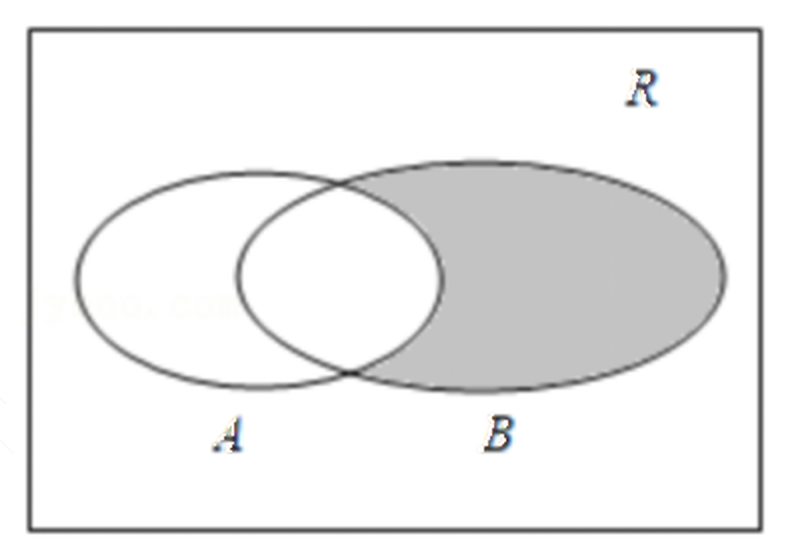
\includegraphics[width=0.36\textwidth]{figures/gao127_q4.png}
\end{center}

\ifanswer
\solbegin
\step{已知 $\R$ 是实数集，集合 $A=\{x\mid 1<x<2\}$, $B=\left\{x\mid 0<x<\frac32\right\}$,}
\step{阴影部分表示的集合是 $\overline A\cap B=\{x\mid 0<x\leqslant1\}$，即 $(0,1]$.}
\solend
\fi

\item 若集合 $\{x\mid (a-1)x^2+3x-2=0\}$ 有且仅有两个子集，则实数 $a$ 的值为\blankline[4.4em].

\ifanswer
\solbegin
\step{由题意得 $\{x\mid (a-1)x^2+3x-2=0\}$ 为单元素集，}
\step{所以 $a-1=0$ 或 $\begin{cases}a-1\neq0\\\triangle=9+8(a-1)=0\end{cases}$，所以 $a=1$ 或 $a=-\frac18$.}
\solend
\fi

\item 已知条件 $\alpha:x\leqslant m$，条件 $\beta:x^2-x\leqslant0$，若 $\alpha$ 是 $\beta$ 的必要条件，则实数 $m$ 的取值范围是为\blankline[4.4em].

\ifanswer
\solbegin
\step{不等式 $x^2-x\leqslant0$ 的解集为 $[0,1]$，}
\step{因为条件 $\alpha:x\leqslant m$，条件 $\beta:x^2-x\leqslant0$，且 $\alpha$ 是 $\beta$ 的必要条件，}
\step{所以集合 $[0,1]$ 是集合 $(-\infty,m]$ 的子集，得 $m\geqslant1$，实数 $m$ 的取值范围是 $[1,+\infty)$.}
\solend
\fi

\item 已知 $\alpha\in\{-2,-1,-\frac12,0,1,2\}$，若幂函数 $y=x^\alpha$ 在 $(0,+\infty)$ 是严格减函数且图像关于 $y$ 轴对称，则 $\alpha=$\blankline[4.4em].

\ifanswer
\solbegin
\step{幂函数 $y=x^\alpha$ 在 $(0,+\infty)$ 是严格减函数，则 $\alpha<0$，且图像关于 $y$ 轴对称，}
\step{则函数为偶函数，故 $\alpha=-2$.}
\solend
\fi

\item 若关于 $x$ 的不等式 $ax^2-3x+2<0$ 的解集不是空集，则实数 $a$ 的取值范围是\blankline[4.4em].

\ifanswer
\solbegin
\step{若 $a>0$，关于 $x$ 的不等式 $ax^2-3x+2<0$ 的解集不空，}
\step{所以一元二次方程 $ax^2-3x+2=0$ 的判别式大于零，}
\step{即 $(-3)^2-8a>0\Rightarrow a<\frac98$，结合 $a>0$ 得 $0<a<\frac98$；}
\step{若 $a\leqslant0$，则关于 $x$ 的不等式 $ax^2-3x+2<0$ 的解集不是空集；}
\step{综上，实数 $a$ 的取值范围是 $\left(-\infty,\frac98\right)$.}
\solend
\fi

\item 设 $\log_{18}2=a$，则 $\log_2 3$ 可用 $a$ 表示为\blankline[4.4em].

\ifanswer
\solbegin
\step{因为 $\log_{18}2=\frac{\log_2 2}{\log_2 18}=\frac1{1+2\log_2 3}=a$，则 $\log_2 3=\frac{1-a}{2a}$.}
\solend
\fi

\item 若关于 $x$ 的不等式 $ax^2+bx+c>0$ 解集为 $\left(-\frac12,3\right)$，则关于 $x$ 的不等式 $cx^2+bx+a<0$ 的解集为\blankline[4.4em].

\ifanswer
\solbegin
\step{由已知得 $a<0$，且 $ax^2+bx+c=a\left(x+\frac12\right)(x-3)$，}
\step{所以 $b=-\frac52 a, c=-\frac32 a$，}
\step{$cx^2+bx+a=-\frac a2(3x-1)(x+2)<0\Leftrightarrow(3x-1)(x+2)<0\Leftrightarrow -2<x<\frac13$，}
\step{故解集为 $\left(-2,\frac13\right)$.}
\solend
\fi

\item 设 $x\in\R$，则方程 $\lvert 2x+3\rvert-\lvert x-2\rvert=\lvert 3x+1\rvert$ 的解集为\blankline[4.4em].

\ifanswer
\solbegin
\step{当 $x\leqslant-\frac32$ 时，原式 $\Leftrightarrow -2x-3+x-2=-3x-1\Leftrightarrow x=2$，不合题意；}
\step{当 $-\frac32<x\leqslant-\frac13$ 时，原式 $\Leftrightarrow 2x+3+x-2=-3x-1\Leftrightarrow x=-\frac13$；}
\step{当 $-\frac13<x\leqslant2$ 时，原式 $\Leftrightarrow 2x+3+x-2=3x+1\Leftrightarrow 1=1$ 即恒成立；}
\step{当 $x>2$ 时，原式 $\Leftrightarrow 2x+3+2-x=3x+1\Leftrightarrow x=2$，不合题意；}
\step{故 $x\in\left[-\frac13,2\right]$.}
\solend
\fi

\item 若关于 $x$ 的不等式 $x^2-4mx+m<0$ 的解集为 $(x_1,x_2)$，若 $x_1>0,x_2>0$，试探究 $x_1+x_2,x_1x_2,x_1^2+x_2^2,\frac1{x_1}+\frac1{x_2}$ 的值，则 $4x_1+x_2$ 的最小值为\blankline[4.4em].

\ifanswer
\solbegin
\step{由题意得方程 $x^2-4mx+m=0$ 有两个相异的正实根 $x_1,x_2$，}
\step{故有 $\begin{cases}\triangle=16m^2-4m>0\\x_1+x_2=4m>0\\x_1\cdot x_2=m>0\end{cases}$，解得 $m>\frac14$，}
\step{则 $x_1^2+x_2^2=(x_1+x_2)^2-2x_1\cdot x_2=16m^2-2m$，$\frac1{x_1}+\frac1{x_2}=\frac{x_1+x_2}{x_1\cdot x_2}=4$，}
\step{则 $4x_1+x_2=\frac14(4x_1+x_2)\left(\frac1{x_1}+\frac1{x_2}\right)=\frac14\left(5+\frac{4x_1}{x_2}+\frac{x_2}{x_1}\right)\geqslant\frac94$，}
\step{当且仅当 $\frac{4x_1}{x_2}=\frac{x_2}{x_1}$ 时，即 $x_2=2x_1$ 时取等号，}
\step{由 $\begin{cases}x_2=2x_1\\\frac1{x_1}+\frac1{x_2}=4\end{cases}$，解得 $\begin{cases}x_1=\frac38\\x_2=\frac34\end{cases}$，于是 $m=x_1\cdot x_2=\frac9{32}\in\left(\frac14,+\infty\right)$，}
\step{即当 $m=\frac9{32}$ 时，$4x_1+x_2$ 取得最小值为 $\frac94$.}
\solend
\fi

\end{enumerate}

\bigsec{二、选择题}

\begin{enumerate}
\setcounter{enumi}{12}

\item 若 $a>0$, $a\neq1$, $M>0$, $N>0$，下列运算正确的是\mbox{（\quad）}

\keepwithprev
A. $\log_a\sqrt[N]{M}=\frac1N\log_a M$\qquad\qquad B. $(\log_a M)^N=N\log_a M$

C. $(\log_a M)\div(\log_a N)=\log_a(M-N)$\qquad\quad D. $\log_a M+\log_a N=\log_a(M+N)$

\ifanswer
\solbegin
\step{对于 $A$，$\log_a\sqrt[N]{M}=\log_a M^{\frac1N}=\frac1N\log_a M$，故 $A$ 正确；}
\step{对于 $B$，$(\log_a M)^N\neq N\log_a M=log_a M^n$，故 $B$ 错误；}
\step{对于 $C$，$(\log_a M)\div(\log_a N)\neq\log_a(M-N)$，故 $C$ 错误；}
\step{对于 $D$，$\log_a M+\log_a N=\log_a MN\neq\log_a(M+N)$，故 $D$ 错误.}
\step{故选 $A$.}
\solend
\fi

\item 下列不等式中正确的是\mbox{（\quad）}

\keepwithprev
A. 若 $a>b$，则 $ac^2>bc^2$\qquad\qquad B. 若 $a<b<0$，则 $a^2<b^2$

C. 若 $1<a<2$ 且 $0<b<3$，则 $1<a+b<5$\qquad D. 若 $\frac1a<1$，则 $a>1$

\ifanswer
\solbegin
\step{$C$ 中 $1+0<a+b<2+3$，即 $1<a+b<5$，正确.}
\step{$A$ 取 $c=0$ 时不成立；$B$ 应为 $a^2>b^2$；$D$ 取 $a=-1$ 时不成立. 故选 $C$.}
\solend
\fi

\item 已知 $y_1=x^3,y_2=x^2$，则下列说法正确的是\mbox{（\quad）}

\keepwithprev
A. $x\in(0,+\infty)$ 时，恒有 $y_1\geqslant y_2$

B. $y_1=x^3$ 与 $y_2=x^2$ 的函数图象仅有唯一交点

C. $x\in(0,1)$ 时，$y_1=x^3$ 图象在 $y_2=x^2$ 图象下方

D. 存在 $x_0\in(1,+\infty)$ 使得 $y_1=y_2$

\ifanswer
\solbegin
\step{$y_1-y_2=x^2(x-1)$，当 $0<x<1$ 时，$y_1<y_2$，故 $C$ 正确，$A$ 错误.}
\step{$y_1=y_2\Leftrightarrow x^2(x-1)=0\Leftrightarrow x=0$ 或 $x=1$，两图象有两个交点，故 $BD$ 错误.}
\step{故选 $C$.}
\solend
\fi

\item 已知非空集合 $A$、$B$ 满足两个条件：(1) $A\cup B=\{1,2,3,4,5,6,7\}$, $A\cap B=\varnothing$；(2) 若 $x\in A$，则 $x+1\in B$，则有序集合对 $(A,B)$ 的个数为\mbox{（\quad）}

\keepwithprev
A. $17$\qquad\qquad B. $18$\qquad\qquad C. $19$\qquad\qquad D. $20$

\ifanswer
\solbegin
\step{当 $A$ 为单元素集合时，有 6 种情况：}
\step{当 $A$ 为双元素集合时，$A=\{1,3\}, A=\{1,4\}, A=\{1,5\}, A=\{1,6\}, A=\{2,4\}$,}
\step{$A=\{2,5\}, A=\{2,6\}, A=\{3,5\}, A=\{3,6\}, A=\{4,6\}$，共 10 种情况；}
\step{当 $A$ 为三元素集合时，$A=\{1,3,5\}, A=\{1,3,6\}, A=\{1,4,6\}, A=\{2,4,6\}$，}
\step{共 4 种情况；}
\step{当 $A$ 为四元素集合时，不成立；}
\step{故有序集合对 $(A,B)$ 的个数为 20，故选 $D$.}
\solend
\fi

\end{enumerate}

\bigsec{三、解答题}

\begin{enumerate}
\setcounter{enumi}{16}

\item 已知 $x,y\in\R$，比较 $x^2+y^2$ 与 $2(2x-y)-5$ 的大小.

\ifanswer
\solbegin
\step{因为 $x^2+y^2-2(2x-y)+5=(x-2)^2+(y+1)^2\geqslant0$，}
\step{所以 $x^2+y^2\geqslant2(2x-y)-5$.}
\solend
\fi

\item 已知集合 $A=\{x\mid x^2+4x=0\}$，$B=\{x\mid x^2+2(a+1)x+a^2-1=0\}$.

(1) 若 $A$ 是 $B$ 的子集，求实数 $a$ 的值；

(2) 若 $B$ 是 $A$ 的子集，求实数 $a$ 的取值范围.

\ifanswer
\solbegin
\step{(1) 因为 $A=\{-4,0\}$，$B=\{x\mid x^2+2(a+1)x+a^2-1=0\}$，又 $A\subseteq B$，}
\step{所以 $A=B$，所以 $\begin{cases}-4+0=-2(a+1)\\-4\times0=a^2-1\end{cases}$，所以 $a=1$；}
\step{(2) 因为 $B$ 是 $A$ 的子集，所以 $B=\varnothing$ 或 $B=\{-4\}$ 或 $B=\{0\}$ 或 $B=\{-4,0\}$，}
\step{① $B=\varnothing$ 时，$\triangle=4(a+1)^2-4(a^2-1)<0$，所以 $a<-1$；}
\step{② $B=\{-4\}$ 时，$\begin{cases}-4+(-4)=-2(a+1)\\-4\times(-4)=a^2-1\end{cases}$，无解；}
\step{③ $B=\{0\}$ 时，$\begin{cases}0+0=-2(a+1)\\0\times0=a^2-1\end{cases}$，所以 $a=-1$；}
\step{④ $B=\{-4,0\}$ 时，由 (1) 得 $a=1$，}
\step{综上，实数 $a$ 的取值范围为 $(-\infty,-1]\cup\{1\}$.}
\solend
\fi

\item 某企业在现有设备下每日生产原先成本 $y$（单位：万元）与日产量 $x$（单位：吨）之间的函数关系式：$y=2x^2+(15-4k)x+120k+8$，近年来各部门都非常重视大气污染防治工作，为了配合环境卫生综合整治，该企业引进了除尘设备，每吨产品的除尘费用为 $k$ 万元，引进除尘设备后，当日产量 $x=1$ 时，总成本（总成本为原先成本和除尘费用之和）为 142 万元.

(1) 求 $k$ 的值；

(2) 求引进除尘设备后日产量为多少时，每吨产品的成本最小，并求出最小值.

\ifanswer
\solbegin
\step{(1) 该企业引进了除尘设备，}
\step{每日生产总成本 $h$（单位：万元）与日产量 $x$（单位：吨）之间的关系为}
\step{$h=2x^2+(15-4k)x+120k+8+kx=2x^2+(15-3k)x+120k+8$，}
\step{当日产量 $x=1$ 时，总成本为 $h=142$ 万元，}
\step{代入得 $2+(15-3k)+120k+8=142\Rightarrow k=1$，}
\step{(2) 由 (1) 得 $h=2x^2+12x+128$，}
\step{所以每吨产品的成本为 $w=\frac{2x^2+12x+128}{x}=2x+\frac{128}{x}+12$}
\step{$\geqslant2\sqrt{2x\cdot\frac{128}{x}}+12=44$，当且仅当 $2x=\frac{128}{x}$，即 $x=8$ 时，取等号，}
\step{所以引进除尘设备后日产量为 8 吨时，每吨产品的成本最小，}
\step{且最小值为 44 万元.}
\solend
\fi

\item 已知集合 $A=\{x\mid \lvert x-a\rvert<2\}$，集合 $B=\left\{x\mid\frac{2x-1}{x+2}<1\right\}$.

(1) 若 $a=2$，求 $A\cup B$；

(2) 若 $A\cap B=A$，求实数 $a$ 的取值范围.

\ifanswer
\solbegin
\step{(1) 若 $a=2$，则 $A=\{x\mid \lvert x-a\rvert<2\}=\{x\mid \lvert x-2\rvert<2\}=\{x\mid 0<x<4\}$，}
\step{由 $\frac{2x-1}{x+2}<1$ 得 $\frac{x-3}{x+2}<0$，即 $(x-3)(x+2)<0$，解得 $-2<x<3$，}
\step{所以 $B=\{x\mid -2<x<3\}$，所以 $A\cup B=\{x\mid -2<x<4\}$；}
\step{(2) 由 (1) 得 $B=\{x\mid -2<x<3\}$，}
\step{$A=\{x\mid \lvert x-a\rvert<2\}=\{x\mid a-2<x<a+2\}$，}
\step{若 $A\cap B=A$，则 $A\subseteq B$，则 $\begin{cases}a-2\geqslant-2\\a+2\leqslant3\end{cases}$，解得 $0\leqslant a\leqslant1$，}
\step{即实数 $a$ 的取值范围为 $[0,1]$.}
\solend
\fi

\item 已知自变量为 $x$ 的函数 $y=\frac{ax+b}{x+a}$，

(1) 若 $a=1$ 且 $b=2$，则函数 $y=\frac{ax+b}{x+a}$ 图像可由幂函数\blankline[4.4em]（写解析式）先沿 $x$ 轴方向\blankline[4.4em]平移\blankline[4.4em]个单位，再沿 $y$ 轴方向向上平移\blankline[4.4em]个单位得到；

(2) 当 $a>0$ 且 $b=-2$ 时不等式 $\frac{ax+b}{x+a}\leqslant\frac{2x^2}{x+a}$ 对 $x>0$ 恒成立，求实数 $a$ 的最大值；

(3) 若 $b=-2$ 且关于 $x$ 的不等式 $x^2\log_2\frac{4(a+1)}a+2x\log_2\frac{2a}{a+1}+\log_2\frac{(a+1)^2}{4a^2}\leqslant0$ 解集是单元素集，求出 $a$ 值，并求出函数 $y=\frac{ax-2}{x+a}$ 的对称中心.

\ifanswer
\solbegin
\step{(1) 已知自变量为 $x$ 的函数 $y=\frac{ax+b}{x+a}$，}
\step{当 $a=1$ 且 $b=2$ 时，$y=\frac{x+2}{x+1}=\frac{x+1+1}{x+1}=1+\frac1{x+1}$，}
\step{由幂函数 $y=\frac1x$，先沿 $x$ 轴方向向左平移一个单位，}
\step{再沿 $y$ 轴方向向上平移一个单位得到；}
\step{(2) 当 $a>0$ 且 $b=-2$ 时不等式 $\frac{ax+b}{x+a}\leqslant\frac{2x^2}{x+a}$ 即 $\frac{ax-2}{x+a}\leqslant\frac{2x^2}{x+a}$ 对 $x>0$ 恒成立，}
\step{因为 $a>0$ 且 $x>0$，所以 $x+a>0$，所以等价于 $ax-2\leqslant2x^2$ 对 $x>0$ 恒成立，}
\step{即 $2x^2-ax+2\geqslant0$ 对 $x>0$ 恒成立，}
\step{因为函数 $g(x)=2x^2-ax+2$ 的对称轴 $x=\frac a4>0$，且 $g(0)=2>0$，}
\step{则 $\begin{cases}\triangle=(-a)^2-4\times2\times2\leqslant0\\a>0\end{cases}$，解得 $0<a\leqslant4$，所以 $a$ 的最大值为 4；}
\step{(3) 关于 $x$ 的不等式 $x^2\log_2\frac{4(a+1)}a+2x\log_2\frac{2a}{a+1}+\log_2\frac{(a+1)^2}{4a^2}\leqslant0$ 解集}
\step{是单元素集，由 $\frac{4(a+1)}a>0$，则 $a>0$ 或 $a<-1$，}
\step{若 $\log_2\frac{4(a+1)}a=0$，则 $\frac{4(a+1)}a=1$，解得 $a=-\frac43$，}
\step{此时不等式为 $6x-6\leqslant0$，解得 $x\leqslant1$，不符合题意，}
\step{若 $\log_2\frac{4(a+1)}a>0$，即 $\frac{4(a+1)}a>1$，解得 $a>0$ 或 $a<-\frac43$，}
\step{则 $\triangle=\left(2\log_2\frac{2a}{a+1}\right)^2-4\log_2\frac{4(a+1)}a\cdot\log_2\frac{(a+1)^2}{4a^2}=0$，}
\step{令 $\log_2\frac{2a}{a+1}=t$，则 $t^2-(3-t)(-2t)=0$，解得 $t=0$ 或 $t=6$，}
\step{当 $\log_2\frac{2a}{a+1}=0$，解得 $a=1$，$\log_2\frac{2a}{a+1}=6$，解得 $a=-\frac{32}{31}$(舍去)，所以 $a=1$，}
\step{则函数 $y=\frac{ax-2}{x+a}$ 即为 $y=\frac{x-2}{x+1}=\frac{x+1-3}{x+1}=1+\frac{-3}{x+1}$，}
\step{对称中心为 $(-1,1)$.}
\solend
\fi

\end{enumerate}

\end{document}
"
%
% 原始材料：微信公众号“魔都数学加油站”文章，作者破晓，2026-11-11 18:35 发布；
% 连载“27学年高一127”，原文标题“27学年高一127——2026-2027年上海市南汇一中高一上期中”；
% 原文链接：https://mp.weixin.qq.com/s/nozIwRgeWSKPCPSiqfCm2Q。
% 正文为 9 张 PNG 页（01、02、03、09 为 2560×3620，04、05、06、07、08 为 4762×6735），
% 题目下印有【解析】，为讲评版。题目、解析均据原图转录；
% 卷面粉红色水印“魔都数学加油站”及公众号页脚未录入。全卷仅第 4 题一幅插图。
% 第 09 页只有一行“对称中心为(-1,1).”及水印，是第 08 页末行的续尾页。
%
% 卷首标题：原卷印作“2026-2027 年南汇一中高一上期中”（公众号标题中的“上海市”
% 卷面标题行没有，本稿照卷面），年份区间按全稿惯例排 en dash；原卷未印副标题，
% 本卷为期中卷、跨三章，按题目内容标为“集合与常用逻辑用语、不等式、函数”
% （第 4/5/6/16/18/20 题为集合与常用逻辑用语，第 8/10/11/12/14/17 题为不等式，
% 第 3/7/9/13/15/19/21 题为函数；与 106、125 同为期中复习卷，口径相同）。
%
% 与原卷的排版差异：
%   ① 原文从第 3 题起，填空题编号为 3—12、选择题为 13—16、解答题为 17—21，本稿保留原题号；
%   ② 原卷每题下直接印【解析】，本稿按全稿惯例置于答案版；四道选择题答案均在解析末句
%      “故选 …”，括号内留空、不另提 \ans{}；全卷无只印【答案】或括号内答案的题；
%   ③ 原卷未印副标题，本稿按“知识模块”口径补出；
%   ④ 原卷填空横线按全稿惯例排为 \blankline[4.4em]；选择题括号排 \mbox{（\quad）}、
%      选项段前按惯例加 \keepwithprev；解答题不留作答区（原卷为讲评版，与 109—125 同）；
%      第 21 题 (1) 的四处填空横线亦排 \blankline[4.4em]；
%   ⑤ 原卷数集排斜体 $R$，按全稿惯例改 \R；绝对值排 \lvert…\rvert，集合描述竖线排 \mid；
%      补集记号照原卷上划线排 \overline{A}；不等号一律 \leqslant / \geqslant；
%   ⑥ 第 4 题插图原在题干右侧，本稿按全稿惯例移至题干之后居中排（取原卷截图、
%      去粉色水印后 2× LANCZOS 放大，存 figures/gao127_q4.png），三版都出；
%      并在该题 \item 前加 \needvspace{} 守卫，把题干与插图整块推走；
%   ⑦ 原卷子题编号 (1)(2)(3) 与括号按全稿惯例排；“（单位：万元）”“（写解析式）”
%      用全角括号，第 21 题 (3) 解析“(舍去)”用半角括号，均照录；
%   ⑧ 第 09 页仅一行“对称中心为(-1,1).”为第 08 页末行之续尾，本稿按原卷印刷行
%      另起一条 \step，置于答案版最后一题解析之末。
%
% 子集符号：第 18 题 (1) 解析 $A\subseteq B$、第 20 题 (2) 解析 $A\subseteq B$ 均印有
%   下划线，照录 \subseteq；全卷无 \subset。回原图放大逐处确认。
%
% 判别式字形：本卷 5 处判别式（第 5 题解析 cases 内 $\triangle=9+8(a-1)=0$、
%   第 12 题解析 cases 内 $\triangle=16m^2-4m>0$、第 18 题① $\triangle=4(a+1)^2-4(a^2-1)<0$、
%   第 21 题 (2) cases 内 $\triangle=(-a)^2-4\times2\times2\leqslant0$、
%   第 21 题 (3) $\triangle=\left(2\log_2\frac{2a}{a+1}\right)^2-\cdots=0$）均排等边扁三角，
%   照录 \triangle；逐处回原图全分辨率放大确认，无高三角 $\Delta$（与 高一26 排 $\Delta$ 不同）。
%
% 原卷存疑照录：
%   第 6 题题干作“则实数 $m$ 的取值范围是为____”（“是为”叠用，疑衍一字），照录；
%   第 12 题题干“试探究 $x_1+x_2, x_1x_2, x_1^2+x_2^2, \frac1{x_1}+\frac1{x_2}$ 的值，
%     则 $4x_1+x_2$ 的最小值为____”与后文衔接突兀，照录；
%   第 13 题解析 B 作“$(\log_a M)^N\neq N\log_a M=log_a M^n$”，后一 log 为斜体、
%     指数作小写 $n$，与前式 $N\log_a M$ 及题干 $N$ 不一致，照录；
%   第 13 题解析 A、B、C 三步句末用“；”，D 步句末用“.”，标点不一致，照录；
%   第 15 题解析“故 $BD$ 错误.”两选项字母连写、无顿号，照录；
%   第 7 题题干及解析用“图像”，第 15 题 B、C 及解析用“图象”，全卷两种写法混用，照录未统一；
%   第 21 题 (3) 题干“求出 $a$ 值”（通常作“求出 $a$ 的值”），照录；
%   第 21 题 (3) 解析“解得 $a=1$，$\log_2\frac{2a}{a+1}=6$，解得 $a=-\frac{32}{31}$(舍去)，
%     所以 $a=1$”两个“解得”并列、且舍去值用半角括号，照录；
%   第 09 页“对称中心为(-1,1).”用半角括号与半角句点，照录；
%   第 8 题解析“若 $a\leqslant0$，则关于 $x$ 的不等式 $ax^2-3x+2<0$ 的解集不是空集；”
%     未给理由直接断言，照录；
%   第 18 题 (1) 由 $A\subseteq B$ 直接得 $A=B$，照录。
%
% 行数核对：逐题数 \step 条数，合计 95 条（Q3：1；Q4：2；Q5：2；Q6：3；Q7：2；
% Q8：5；Q9：1；Q10：4；Q11：5；Q12：7；Q13：5；Q14：2；Q15：3；Q16：7；
% Q17：2；Q18：8；Q19：10；Q20：7；Q21：19），与原卷印刷行逐题相等
% （cases 块作一个印刷行计；Q21 第 19 行为第 09 页续尾）。全卷 19 题均印【解析】，
% 无只印【答案】或括号内答案的题，故 \ans{} 为 0；四道选择题括号内留空、不另提 \ans{}。
%
\documentclass[a4paper,11pt]{article}
\usepackage{common}

\begin{document}

\examtitlest[3]{2026--2027 年南汇一中高一上期中}{集合与常用逻辑用语、不等式、函数}

\bigsec{一、填空题}

\begin{enumerate}
\setcounter{enumi}{2}

\item 把 $\sqrt[4]{a\sqrt a}(a>0)$ 化成有理数指数幂的形式为\blankline[4.4em].

\ifanswer
\solbegin
\step{$\sqrt[4]{a\sqrt a}=(a\cdot a^{\frac12})^{\frac14}=a^{\frac38}$.}
\solend
\fi

\needvspace{6.5cm}
\item 已知集合 $A=\{x\mid 1<x<2\}$, $B=\left\{x\mid 0<x<\frac32\right\}$, 则如图阴影部分表示的集合是\blankline[4.4em].

\begin{center}
% 图取原卷截图（第 1 页题干右侧）、去水印后 2× LANCZOS 放大，本稿移至题干之后
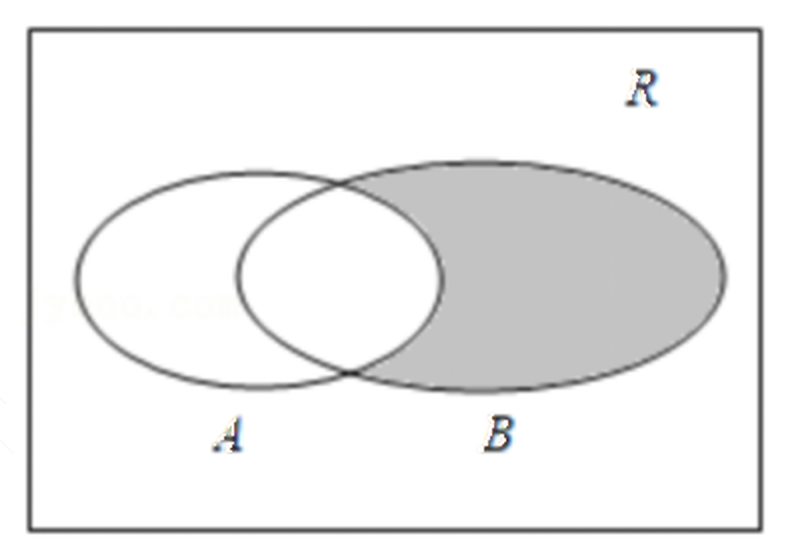
\includegraphics[width=0.36\textwidth]{figures/gao127_q4.png}
\end{center}

\ifanswer
\solbegin
\step{已知 $\R$ 是实数集，集合 $A=\{x\mid 1<x<2\}$, $B=\left\{x\mid 0<x<\frac32\right\}$,}
\step{阴影部分表示的集合是 $\overline A\cap B=\{x\mid 0<x\leqslant1\}$，即 $(0,1]$.}
\solend
\fi

\item 若集合 $\{x\mid (a-1)x^2+3x-2=0\}$ 有且仅有两个子集，则实数 $a$ 的值为\blankline[4.4em].

\ifanswer
\solbegin
\step{由题意得 $\{x\mid (a-1)x^2+3x-2=0\}$ 为单元素集，}
\step{所以 $a-1=0$ 或 $\begin{cases}a-1\neq0\\\triangle=9+8(a-1)=0\end{cases}$，所以 $a=1$ 或 $a=-\frac18$.}
\solend
\fi

\item 已知条件 $\alpha:x\leqslant m$，条件 $\beta:x^2-x\leqslant0$，若 $\alpha$ 是 $\beta$ 的必要条件，则实数 $m$ 的取值范围是为\blankline[4.4em].

\ifanswer
\solbegin
\step{不等式 $x^2-x\leqslant0$ 的解集为 $[0,1]$，}
\step{因为条件 $\alpha:x\leqslant m$，条件 $\beta:x^2-x\leqslant0$，且 $\alpha$ 是 $\beta$ 的必要条件，}
\step{所以集合 $[0,1]$ 是集合 $(-\infty,m]$ 的子集，得 $m\geqslant1$，实数 $m$ 的取值范围是 $[1,+\infty)$.}
\solend
\fi

\item 已知 $\alpha\in\{-2,-1,-\frac12,0,1,2\}$，若幂函数 $y=x^\alpha$ 在 $(0,+\infty)$ 是严格减函数且图像关于 $y$ 轴对称，则 $\alpha=$\blankline[4.4em].

\ifanswer
\solbegin
\step{幂函数 $y=x^\alpha$ 在 $(0,+\infty)$ 是严格减函数，则 $\alpha<0$，且图像关于 $y$ 轴对称，}
\step{则函数为偶函数，故 $\alpha=-2$.}
\solend
\fi

\item 若关于 $x$ 的不等式 $ax^2-3x+2<0$ 的解集不是空集，则实数 $a$ 的取值范围是\blankline[4.4em].

\ifanswer
\solbegin
\step{若 $a>0$，关于 $x$ 的不等式 $ax^2-3x+2<0$ 的解集不空，}
\step{所以一元二次方程 $ax^2-3x+2=0$ 的判别式大于零，}
\step{即 $(-3)^2-8a>0\Rightarrow a<\frac98$，结合 $a>0$ 得 $0<a<\frac98$；}
\step{若 $a\leqslant0$，则关于 $x$ 的不等式 $ax^2-3x+2<0$ 的解集不是空集；}
\step{综上，实数 $a$ 的取值范围是 $\left(-\infty,\frac98\right)$.}
\solend
\fi

\item 设 $\log_{18}2=a$，则 $\log_2 3$ 可用 $a$ 表示为\blankline[4.4em].

\ifanswer
\solbegin
\step{因为 $\log_{18}2=\frac{\log_2 2}{\log_2 18}=\frac1{1+2\log_2 3}=a$，则 $\log_2 3=\frac{1-a}{2a}$.}
\solend
\fi

\item 若关于 $x$ 的不等式 $ax^2+bx+c>0$ 解集为 $\left(-\frac12,3\right)$，则关于 $x$ 的不等式 $cx^2+bx+a<0$ 的解集为\blankline[4.4em].

\ifanswer
\solbegin
\step{由已知得 $a<0$，且 $ax^2+bx+c=a\left(x+\frac12\right)(x-3)$，}
\step{所以 $b=-\frac52 a, c=-\frac32 a$，}
\step{$cx^2+bx+a=-\frac a2(3x-1)(x+2)<0\Leftrightarrow(3x-1)(x+2)<0\Leftrightarrow -2<x<\frac13$，}
\step{故解集为 $\left(-2,\frac13\right)$.}
\solend
\fi

\item 设 $x\in\R$，则方程 $\lvert 2x+3\rvert-\lvert x-2\rvert=\lvert 3x+1\rvert$ 的解集为\blankline[4.4em].

\ifanswer
\solbegin
\step{当 $x\leqslant-\frac32$ 时，原式 $\Leftrightarrow -2x-3+x-2=-3x-1\Leftrightarrow x=2$，不合题意；}
\step{当 $-\frac32<x\leqslant-\frac13$ 时，原式 $\Leftrightarrow 2x+3+x-2=-3x-1\Leftrightarrow x=-\frac13$；}
\step{当 $-\frac13<x\leqslant2$ 时，原式 $\Leftrightarrow 2x+3+x-2=3x+1\Leftrightarrow 1=1$ 即恒成立；}
\step{当 $x>2$ 时，原式 $\Leftrightarrow 2x+3+2-x=3x+1\Leftrightarrow x=2$，不合题意；}
\step{故 $x\in\left[-\frac13,2\right]$.}
\solend
\fi

\item 若关于 $x$ 的不等式 $x^2-4mx+m<0$ 的解集为 $(x_1,x_2)$，若 $x_1>0,x_2>0$，试探究 $x_1+x_2,x_1x_2,x_1^2+x_2^2,\frac1{x_1}+\frac1{x_2}$ 的值，则 $4x_1+x_2$ 的最小值为\blankline[4.4em].

\ifanswer
\solbegin
\step{由题意得方程 $x^2-4mx+m=0$ 有两个相异的正实根 $x_1,x_2$，}
\step{故有 $\begin{cases}\triangle=16m^2-4m>0\\x_1+x_2=4m>0\\x_1\cdot x_2=m>0\end{cases}$，解得 $m>\frac14$，}
\step{则 $x_1^2+x_2^2=(x_1+x_2)^2-2x_1\cdot x_2=16m^2-2m$，$\frac1{x_1}+\frac1{x_2}=\frac{x_1+x_2}{x_1\cdot x_2}=4$，}
\step{则 $4x_1+x_2=\frac14(4x_1+x_2)\left(\frac1{x_1}+\frac1{x_2}\right)=\frac14\left(5+\frac{4x_1}{x_2}+\frac{x_2}{x_1}\right)\geqslant\frac94$，}
\step{当且仅当 $\frac{4x_1}{x_2}=\frac{x_2}{x_1}$ 时，即 $x_2=2x_1$ 时取等号，}
\step{由 $\begin{cases}x_2=2x_1\\\frac1{x_1}+\frac1{x_2}=4\end{cases}$，解得 $\begin{cases}x_1=\frac38\\x_2=\frac34\end{cases}$，于是 $m=x_1\cdot x_2=\frac9{32}\in\left(\frac14,+\infty\right)$，}
\step{即当 $m=\frac9{32}$ 时，$4x_1+x_2$ 取得最小值为 $\frac94$.}
\solend
\fi

\end{enumerate}

\bigsec{二、选择题}

\begin{enumerate}
\setcounter{enumi}{12}

\item 若 $a>0$, $a\neq1$, $M>0$, $N>0$，下列运算正确的是\mbox{（\quad）}

\keepwithprev
A. $\log_a\sqrt[N]{M}=\frac1N\log_a M$\qquad\qquad B. $(\log_a M)^N=N\log_a M$

C. $(\log_a M)\div(\log_a N)=\log_a(M-N)$\qquad\quad D. $\log_a M+\log_a N=\log_a(M+N)$

\ifanswer
\solbegin
\step{对于 $A$，$\log_a\sqrt[N]{M}=\log_a M^{\frac1N}=\frac1N\log_a M$，故 $A$ 正确；}
\step{对于 $B$，$(\log_a M)^N\neq N\log_a M=log_a M^n$，故 $B$ 错误；}
\step{对于 $C$，$(\log_a M)\div(\log_a N)\neq\log_a(M-N)$，故 $C$ 错误；}
\step{对于 $D$，$\log_a M+\log_a N=\log_a MN\neq\log_a(M+N)$，故 $D$ 错误.}
\step{故选 $A$.}
\solend
\fi

\item 下列不等式中正确的是\mbox{（\quad）}

\keepwithprev
A. 若 $a>b$，则 $ac^2>bc^2$\qquad\qquad B. 若 $a<b<0$，则 $a^2<b^2$

C. 若 $1<a<2$ 且 $0<b<3$，则 $1<a+b<5$\qquad D. 若 $\frac1a<1$，则 $a>1$

\ifanswer
\solbegin
\step{$C$ 中 $1+0<a+b<2+3$，即 $1<a+b<5$，正确.}
\step{$A$ 取 $c=0$ 时不成立；$B$ 应为 $a^2>b^2$；$D$ 取 $a=-1$ 时不成立. 故选 $C$.}
\solend
\fi

\item 已知 $y_1=x^3,y_2=x^2$，则下列说法正确的是\mbox{（\quad）}

\keepwithprev
A. $x\in(0,+\infty)$ 时，恒有 $y_1\geqslant y_2$

B. $y_1=x^3$ 与 $y_2=x^2$ 的函数图象仅有唯一交点

C. $x\in(0,1)$ 时，$y_1=x^3$ 图象在 $y_2=x^2$ 图象下方

D. 存在 $x_0\in(1,+\infty)$ 使得 $y_1=y_2$

\ifanswer
\solbegin
\step{$y_1-y_2=x^2(x-1)$，当 $0<x<1$ 时，$y_1<y_2$，故 $C$ 正确，$A$ 错误.}
\step{$y_1=y_2\Leftrightarrow x^2(x-1)=0\Leftrightarrow x=0$ 或 $x=1$，两图象有两个交点，故 $BD$ 错误.}
\step{故选 $C$.}
\solend
\fi

\item 已知非空集合 $A$、$B$ 满足两个条件：(1) $A\cup B=\{1,2,3,4,5,6,7\}$, $A\cap B=\varnothing$；(2) 若 $x\in A$，则 $x+1\in B$，则有序集合对 $(A,B)$ 的个数为\mbox{（\quad）}

\keepwithprev
A. $17$\qquad\qquad B. $18$\qquad\qquad C. $19$\qquad\qquad D. $20$

\ifanswer
\solbegin
\step{当 $A$ 为单元素集合时，有 6 种情况：}
\step{当 $A$ 为双元素集合时，$A=\{1,3\}, A=\{1,4\}, A=\{1,5\}, A=\{1,6\}, A=\{2,4\}$,}
\step{$A=\{2,5\}, A=\{2,6\}, A=\{3,5\}, A=\{3,6\}, A=\{4,6\}$，共 10 种情况；}
\step{当 $A$ 为三元素集合时，$A=\{1,3,5\}, A=\{1,3,6\}, A=\{1,4,6\}, A=\{2,4,6\}$，}
\step{共 4 种情况；}
\step{当 $A$ 为四元素集合时，不成立；}
\step{故有序集合对 $(A,B)$ 的个数为 20，故选 $D$.}
\solend
\fi

\end{enumerate}

\bigsec{三、解答题}

\begin{enumerate}
\setcounter{enumi}{16}

\item 已知 $x,y\in\R$，比较 $x^2+y^2$ 与 $2(2x-y)-5$ 的大小.

\ifanswer
\solbegin
\step{因为 $x^2+y^2-2(2x-y)+5=(x-2)^2+(y+1)^2\geqslant0$，}
\step{所以 $x^2+y^2\geqslant2(2x-y)-5$.}
\solend
\fi

\item 已知集合 $A=\{x\mid x^2+4x=0\}$，$B=\{x\mid x^2+2(a+1)x+a^2-1=0\}$.

(1) 若 $A$ 是 $B$ 的子集，求实数 $a$ 的值；

(2) 若 $B$ 是 $A$ 的子集，求实数 $a$ 的取值范围.

\ifanswer
\solbegin
\step{(1) 因为 $A=\{-4,0\}$，$B=\{x\mid x^2+2(a+1)x+a^2-1=0\}$，又 $A\subseteq B$，}
\step{所以 $A=B$，所以 $\begin{cases}-4+0=-2(a+1)\\-4\times0=a^2-1\end{cases}$，所以 $a=1$；}
\step{(2) 因为 $B$ 是 $A$ 的子集，所以 $B=\varnothing$ 或 $B=\{-4\}$ 或 $B=\{0\}$ 或 $B=\{-4,0\}$，}
\step{① $B=\varnothing$ 时，$\triangle=4(a+1)^2-4(a^2-1)<0$，所以 $a<-1$；}
\step{② $B=\{-4\}$ 时，$\begin{cases}-4+(-4)=-2(a+1)\\-4\times(-4)=a^2-1\end{cases}$，无解；}
\step{③ $B=\{0\}$ 时，$\begin{cases}0+0=-2(a+1)\\0\times0=a^2-1\end{cases}$，所以 $a=-1$；}
\step{④ $B=\{-4,0\}$ 时，由 (1) 得 $a=1$，}
\step{综上，实数 $a$ 的取值范围为 $(-\infty,-1]\cup\{1\}$.}
\solend
\fi

\item 某企业在现有设备下每日生产原先成本 $y$（单位：万元）与日产量 $x$（单位：吨）之间的函数关系式：$y=2x^2+(15-4k)x+120k+8$，近年来各部门都非常重视大气污染防治工作，为了配合环境卫生综合整治，该企业引进了除尘设备，每吨产品的除尘费用为 $k$ 万元，引进除尘设备后，当日产量 $x=1$ 时，总成本（总成本为原先成本和除尘费用之和）为 142 万元.

(1) 求 $k$ 的值；

(2) 求引进除尘设备后日产量为多少时，每吨产品的成本最小，并求出最小值.

\ifanswer
\solbegin
\step{(1) 该企业引进了除尘设备，}
\step{每日生产总成本 $h$（单位：万元）与日产量 $x$（单位：吨）之间的关系为}
\step{$h=2x^2+(15-4k)x+120k+8+kx=2x^2+(15-3k)x+120k+8$，}
\step{当日产量 $x=1$ 时，总成本为 $h=142$ 万元，}
\step{代入得 $2+(15-3k)+120k+8=142\Rightarrow k=1$，}
\step{(2) 由 (1) 得 $h=2x^2+12x+128$，}
\step{所以每吨产品的成本为 $w=\frac{2x^2+12x+128}{x}=2x+\frac{128}{x}+12$}
\step{$\geqslant2\sqrt{2x\cdot\frac{128}{x}}+12=44$，当且仅当 $2x=\frac{128}{x}$，即 $x=8$ 时，取等号，}
\step{所以引进除尘设备后日产量为 8 吨时，每吨产品的成本最小，}
\step{且最小值为 44 万元.}
\solend
\fi

\item 已知集合 $A=\{x\mid \lvert x-a\rvert<2\}$，集合 $B=\left\{x\mid\frac{2x-1}{x+2}<1\right\}$.

(1) 若 $a=2$，求 $A\cup B$；

(2) 若 $A\cap B=A$，求实数 $a$ 的取值范围.

\ifanswer
\solbegin
\step{(1) 若 $a=2$，则 $A=\{x\mid \lvert x-a\rvert<2\}=\{x\mid \lvert x-2\rvert<2\}=\{x\mid 0<x<4\}$，}
\step{由 $\frac{2x-1}{x+2}<1$ 得 $\frac{x-3}{x+2}<0$，即 $(x-3)(x+2)<0$，解得 $-2<x<3$，}
\step{所以 $B=\{x\mid -2<x<3\}$，所以 $A\cup B=\{x\mid -2<x<4\}$；}
\step{(2) 由 (1) 得 $B=\{x\mid -2<x<3\}$，}
\step{$A=\{x\mid \lvert x-a\rvert<2\}=\{x\mid a-2<x<a+2\}$，}
\step{若 $A\cap B=A$，则 $A\subseteq B$，则 $\begin{cases}a-2\geqslant-2\\a+2\leqslant3\end{cases}$，解得 $0\leqslant a\leqslant1$，}
\step{即实数 $a$ 的取值范围为 $[0,1]$.}
\solend
\fi

\item 已知自变量为 $x$ 的函数 $y=\frac{ax+b}{x+a}$，

(1) 若 $a=1$ 且 $b=2$，则函数 $y=\frac{ax+b}{x+a}$ 图像可由幂函数\blankline[4.4em]（写解析式）先沿 $x$ 轴方向\blankline[4.4em]平移\blankline[4.4em]个单位，再沿 $y$ 轴方向向上平移\blankline[4.4em]个单位得到；

(2) 当 $a>0$ 且 $b=-2$ 时不等式 $\frac{ax+b}{x+a}\leqslant\frac{2x^2}{x+a}$ 对 $x>0$ 恒成立，求实数 $a$ 的最大值；

(3) 若 $b=-2$ 且关于 $x$ 的不等式 $x^2\log_2\frac{4(a+1)}a+2x\log_2\frac{2a}{a+1}+\log_2\frac{(a+1)^2}{4a^2}\leqslant0$ 解集是单元素集，求出 $a$ 值，并求出函数 $y=\frac{ax-2}{x+a}$ 的对称中心.

\ifanswer
\solbegin
\step{(1) 已知自变量为 $x$ 的函数 $y=\frac{ax+b}{x+a}$，}
\step{当 $a=1$ 且 $b=2$ 时，$y=\frac{x+2}{x+1}=\frac{x+1+1}{x+1}=1+\frac1{x+1}$，}
\step{由幂函数 $y=\frac1x$，先沿 $x$ 轴方向向左平移一个单位，}
\step{再沿 $y$ 轴方向向上平移一个单位得到；}
\step{(2) 当 $a>0$ 且 $b=-2$ 时不等式 $\frac{ax+b}{x+a}\leqslant\frac{2x^2}{x+a}$ 即 $\frac{ax-2}{x+a}\leqslant\frac{2x^2}{x+a}$ 对 $x>0$ 恒成立，}
\step{因为 $a>0$ 且 $x>0$，所以 $x+a>0$，所以等价于 $ax-2\leqslant2x^2$ 对 $x>0$ 恒成立，}
\step{即 $2x^2-ax+2\geqslant0$ 对 $x>0$ 恒成立，}
\step{因为函数 $g(x)=2x^2-ax+2$ 的对称轴 $x=\frac a4>0$，且 $g(0)=2>0$，}
\step{则 $\begin{cases}\triangle=(-a)^2-4\times2\times2\leqslant0\\a>0\end{cases}$，解得 $0<a\leqslant4$，所以 $a$ 的最大值为 4；}
\step{(3) 关于 $x$ 的不等式 $x^2\log_2\frac{4(a+1)}a+2x\log_2\frac{2a}{a+1}+\log_2\frac{(a+1)^2}{4a^2}\leqslant0$ 解集}
\step{是单元素集，由 $\frac{4(a+1)}a>0$，则 $a>0$ 或 $a<-1$，}
\step{若 $\log_2\frac{4(a+1)}a=0$，则 $\frac{4(a+1)}a=1$，解得 $a=-\frac43$，}
\step{此时不等式为 $6x-6\leqslant0$，解得 $x\leqslant1$，不符合题意，}
\step{若 $\log_2\frac{4(a+1)}a>0$，即 $\frac{4(a+1)}a>1$，解得 $a>0$ 或 $a<-\frac43$，}
\step{则 $\triangle=\left(2\log_2\frac{2a}{a+1}\right)^2-4\log_2\frac{4(a+1)}a\cdot\log_2\frac{(a+1)^2}{4a^2}=0$，}
\step{令 $\log_2\frac{2a}{a+1}=t$，则 $t^2-(3-t)(-2t)=0$，解得 $t=0$ 或 $t=6$，}
\step{当 $\log_2\frac{2a}{a+1}=0$，解得 $a=1$，$\log_2\frac{2a}{a+1}=6$，解得 $a=-\frac{32}{31}$(舍去)，所以 $a=1$，}
\step{则函数 $y=\frac{ax-2}{x+a}$ 即为 $y=\frac{x-2}{x+1}=\frac{x+1-3}{x+1}=1+\frac{-3}{x+1}$，}
\step{对称中心为 $(-1,1)$.}
\solend
\fi

\end{enumerate}

\end{document}
"
%
% 原始材料：微信公众号“魔都数学加油站”文章，作者破晓，2026-11-11 18:35 发布；
% 连载“27学年高一127”，原文标题“27学年高一127——2026-2027年上海市南汇一中高一上期中”；
% 原文链接：https://mp.weixin.qq.com/s/nozIwRgeWSKPCPSiqfCm2Q。
% 正文为 9 张 PNG 页（01、02、03、09 为 2560×3620，04、05、06、07、08 为 4762×6735），
% 题目下印有【解析】，为讲评版。题目、解析均据原图转录；
% 卷面粉红色水印“魔都数学加油站”及公众号页脚未录入。全卷仅第 4 题一幅插图。
% 第 09 页只有一行“对称中心为(-1,1).”及水印，是第 08 页末行的续尾页。
%
% 卷首标题：原卷印作“2026-2027 年南汇一中高一上期中”（公众号标题中的“上海市”
% 卷面标题行没有，本稿照卷面），年份区间按全稿惯例排 en dash；原卷未印副标题，
% 本卷为期中卷、跨三章，按题目内容标为“集合与常用逻辑用语、不等式、函数”
% （第 4/5/6/16/18/20 题为集合与常用逻辑用语，第 8/10/11/12/14/17 题为不等式，
% 第 3/7/9/13/15/19/21 题为函数；与 106、125 同为期中复习卷，口径相同）。
%
% 与原卷的排版差异：
%   ① 原文从第 3 题起，填空题编号为 3—12、选择题为 13—16、解答题为 17—21，本稿保留原题号；
%   ② 原卷每题下直接印【解析】，本稿按全稿惯例置于答案版；四道选择题答案均在解析末句
%      “故选 …”，括号内留空、不另提 \ans{}；全卷无只印【答案】或括号内答案的题；
%   ③ 原卷未印副标题，本稿按“知识模块”口径补出；
%   ④ 原卷填空横线按全稿惯例排为 \blankline[4.4em]；选择题括号排 \mbox{（\quad）}、
%      选项段前按惯例加 \keepwithprev；解答题不留作答区（原卷为讲评版，与 109—125 同）；
%      第 21 题 (1) 的四处填空横线亦排 \blankline[4.4em]；
%   ⑤ 原卷数集排斜体 $R$，按全稿惯例改 \R；绝对值排 \lvert…\rvert，集合描述竖线排 \mid；
%      补集记号照原卷上划线排 \overline{A}；不等号一律 \leqslant / \geqslant；
%   ⑥ 第 4 题插图原在题干右侧，本稿按全稿惯例移至题干之后居中排（取原卷截图、
%      去粉色水印后 2× LANCZOS 放大，存 figures/gao127_q4.png），三版都出；
%      并在该题 \item 前加 \needvspace{} 守卫，把题干与插图整块推走；
%   ⑦ 原卷子题编号 (1)(2)(3) 与括号按全稿惯例排；“（单位：万元）”“（写解析式）”
%      用全角括号，第 21 题 (3) 解析“(舍去)”用半角括号，均照录；
%   ⑧ 第 09 页仅一行“对称中心为(-1,1).”为第 08 页末行之续尾，本稿按原卷印刷行
%      另起一条 \step，置于答案版最后一题解析之末。
%
% 子集符号：第 18 题 (1) 解析 $A\subseteq B$、第 20 题 (2) 解析 $A\subseteq B$ 均印有
%   下划线，照录 \subseteq；全卷无 \subset。回原图放大逐处确认。
%
% 判别式字形：本卷 5 处判别式（第 5 题解析 cases 内 $\triangle=9+8(a-1)=0$、
%   第 12 题解析 cases 内 $\triangle=16m^2-4m>0$、第 18 题① $\triangle=4(a+1)^2-4(a^2-1)<0$、
%   第 21 题 (2) cases 内 $\triangle=(-a)^2-4\times2\times2\leqslant0$、
%   第 21 题 (3) $\triangle=\left(2\log_2\frac{2a}{a+1}\right)^2-\cdots=0$）均排等边扁三角，
%   照录 \triangle；逐处回原图全分辨率放大确认，无高三角 $\Delta$（与 高一26 排 $\Delta$ 不同）。
%
% 原卷存疑照录：
%   第 6 题题干作“则实数 $m$ 的取值范围是为____”（“是为”叠用，疑衍一字），照录；
%   第 12 题题干“试探究 $x_1+x_2, x_1x_2, x_1^2+x_2^2, \frac1{x_1}+\frac1{x_2}$ 的值，
%     则 $4x_1+x_2$ 的最小值为____”与后文衔接突兀，照录；
%   第 13 题解析 B 作“$(\log_a M)^N\neq N\log_a M=log_a M^n$”，后一 log 为斜体、
%     指数作小写 $n$，与前式 $N\log_a M$ 及题干 $N$ 不一致，照录；
%   第 13 题解析 A、B、C 三步句末用“；”，D 步句末用“.”，标点不一致，照录；
%   第 15 题解析“故 $BD$ 错误.”两选项字母连写、无顿号，照录；
%   第 7 题题干及解析用“图像”，第 15 题 B、C 及解析用“图象”，全卷两种写法混用，照录未统一；
%   第 21 题 (3) 题干“求出 $a$ 值”（通常作“求出 $a$ 的值”），照录；
%   第 21 题 (3) 解析“解得 $a=1$，$\log_2\frac{2a}{a+1}=6$，解得 $a=-\frac{32}{31}$(舍去)，
%     所以 $a=1$”两个“解得”并列、且舍去值用半角括号，照录；
%   第 09 页“对称中心为(-1,1).”用半角括号与半角句点，照录；
%   第 8 题解析“若 $a\leqslant0$，则关于 $x$ 的不等式 $ax^2-3x+2<0$ 的解集不是空集；”
%     未给理由直接断言，照录；
%   第 18 题 (1) 由 $A\subseteq B$ 直接得 $A=B$，照录。
%
% 行数核对：逐题数 \step 条数，合计 95 条（Q3：1；Q4：2；Q5：2；Q6：3；Q7：2；
% Q8：5；Q9：1；Q10：4；Q11：5；Q12：7；Q13：5；Q14：2；Q15：3；Q16：7；
% Q17：2；Q18：8；Q19：10；Q20：7；Q21：19），与原卷印刷行逐题相等
% （cases 块作一个印刷行计；Q21 第 19 行为第 09 页续尾）。全卷 19 题均印【解析】，
% 无只印【答案】或括号内答案的题，故 \ans{} 为 0；四道选择题括号内留空、不另提 \ans{}。
%
\documentclass[a4paper,11pt]{article}
\usepackage{common}

\begin{document}

\examtitlest[3]{2026--2027 年南汇一中高一上期中}{集合与常用逻辑用语、不等式、函数}

\bigsec{一、填空题}

\begin{enumerate}
\setcounter{enumi}{2}

\item 把 $\sqrt[4]{a\sqrt a}(a>0)$ 化成有理数指数幂的形式为\blankline[4.4em].

\ifanswer
\solbegin
\step{$\sqrt[4]{a\sqrt a}=(a\cdot a^{\frac12})^{\frac14}=a^{\frac38}$.}
\solend
\fi

\needvspace{6.5cm}
\item 已知集合 $A=\{x\mid 1<x<2\}$, $B=\left\{x\mid 0<x<\frac32\right\}$, 则如图阴影部分表示的集合是\blankline[4.4em].

\begin{center}
% 图取原卷截图（第 1 页题干右侧）、去水印后 2× LANCZOS 放大，本稿移至题干之后
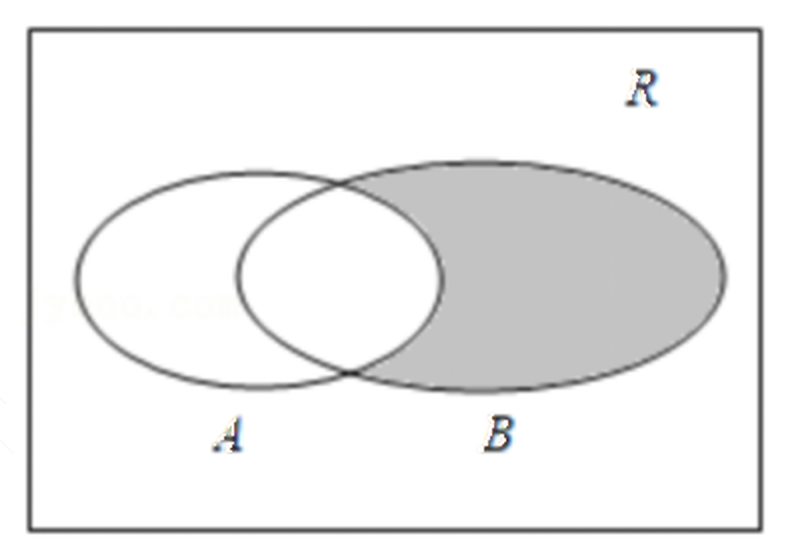
\includegraphics[width=0.36\textwidth]{figures/gao127_q4.png}
\end{center}

\ifanswer
\solbegin
\step{已知 $\R$ 是实数集，集合 $A=\{x\mid 1<x<2\}$, $B=\left\{x\mid 0<x<\frac32\right\}$,}
\step{阴影部分表示的集合是 $\overline A\cap B=\{x\mid 0<x\leqslant1\}$，即 $(0,1]$.}
\solend
\fi

\item 若集合 $\{x\mid (a-1)x^2+3x-2=0\}$ 有且仅有两个子集，则实数 $a$ 的值为\blankline[4.4em].

\ifanswer
\solbegin
\step{由题意得 $\{x\mid (a-1)x^2+3x-2=0\}$ 为单元素集，}
\step{所以 $a-1=0$ 或 $\begin{cases}a-1\neq0\\\triangle=9+8(a-1)=0\end{cases}$，所以 $a=1$ 或 $a=-\frac18$.}
\solend
\fi

\item 已知条件 $\alpha:x\leqslant m$，条件 $\beta:x^2-x\leqslant0$，若 $\alpha$ 是 $\beta$ 的必要条件，则实数 $m$ 的取值范围是为\blankline[4.4em].

\ifanswer
\solbegin
\step{不等式 $x^2-x\leqslant0$ 的解集为 $[0,1]$，}
\step{因为条件 $\alpha:x\leqslant m$，条件 $\beta:x^2-x\leqslant0$，且 $\alpha$ 是 $\beta$ 的必要条件，}
\step{所以集合 $[0,1]$ 是集合 $(-\infty,m]$ 的子集，得 $m\geqslant1$，实数 $m$ 的取值范围是 $[1,+\infty)$.}
\solend
\fi

\item 已知 $\alpha\in\{-2,-1,-\frac12,0,1,2\}$，若幂函数 $y=x^\alpha$ 在 $(0,+\infty)$ 是严格减函数且图像关于 $y$ 轴对称，则 $\alpha=$\blankline[4.4em].

\ifanswer
\solbegin
\step{幂函数 $y=x^\alpha$ 在 $(0,+\infty)$ 是严格减函数，则 $\alpha<0$，且图像关于 $y$ 轴对称，}
\step{则函数为偶函数，故 $\alpha=-2$.}
\solend
\fi

\item 若关于 $x$ 的不等式 $ax^2-3x+2<0$ 的解集不是空集，则实数 $a$ 的取值范围是\blankline[4.4em].

\ifanswer
\solbegin
\step{若 $a>0$，关于 $x$ 的不等式 $ax^2-3x+2<0$ 的解集不空，}
\step{所以一元二次方程 $ax^2-3x+2=0$ 的判别式大于零，}
\step{即 $(-3)^2-8a>0\Rightarrow a<\frac98$，结合 $a>0$ 得 $0<a<\frac98$；}
\step{若 $a\leqslant0$，则关于 $x$ 的不等式 $ax^2-3x+2<0$ 的解集不是空集；}
\step{综上，实数 $a$ 的取值范围是 $\left(-\infty,\frac98\right)$.}
\solend
\fi

\item 设 $\log_{18}2=a$，则 $\log_2 3$ 可用 $a$ 表示为\blankline[4.4em].

\ifanswer
\solbegin
\step{因为 $\log_{18}2=\frac{\log_2 2}{\log_2 18}=\frac1{1+2\log_2 3}=a$，则 $\log_2 3=\frac{1-a}{2a}$.}
\solend
\fi

\item 若关于 $x$ 的不等式 $ax^2+bx+c>0$ 解集为 $\left(-\frac12,3\right)$，则关于 $x$ 的不等式 $cx^2+bx+a<0$ 的解集为\blankline[4.4em].

\ifanswer
\solbegin
\step{由已知得 $a<0$，且 $ax^2+bx+c=a\left(x+\frac12\right)(x-3)$，}
\step{所以 $b=-\frac52 a, c=-\frac32 a$，}
\step{$cx^2+bx+a=-\frac a2(3x-1)(x+2)<0\Leftrightarrow(3x-1)(x+2)<0\Leftrightarrow -2<x<\frac13$，}
\step{故解集为 $\left(-2,\frac13\right)$.}
\solend
\fi

\item 设 $x\in\R$，则方程 $\lvert 2x+3\rvert-\lvert x-2\rvert=\lvert 3x+1\rvert$ 的解集为\blankline[4.4em].

\ifanswer
\solbegin
\step{当 $x\leqslant-\frac32$ 时，原式 $\Leftrightarrow -2x-3+x-2=-3x-1\Leftrightarrow x=2$，不合题意；}
\step{当 $-\frac32<x\leqslant-\frac13$ 时，原式 $\Leftrightarrow 2x+3+x-2=-3x-1\Leftrightarrow x=-\frac13$；}
\step{当 $-\frac13<x\leqslant2$ 时，原式 $\Leftrightarrow 2x+3+x-2=3x+1\Leftrightarrow 1=1$ 即恒成立；}
\step{当 $x>2$ 时，原式 $\Leftrightarrow 2x+3+2-x=3x+1\Leftrightarrow x=2$，不合题意；}
\step{故 $x\in\left[-\frac13,2\right]$.}
\solend
\fi

\item 若关于 $x$ 的不等式 $x^2-4mx+m<0$ 的解集为 $(x_1,x_2)$，若 $x_1>0,x_2>0$，试探究 $x_1+x_2,x_1x_2,x_1^2+x_2^2,\frac1{x_1}+\frac1{x_2}$ 的值，则 $4x_1+x_2$ 的最小值为\blankline[4.4em].

\ifanswer
\solbegin
\step{由题意得方程 $x^2-4mx+m=0$ 有两个相异的正实根 $x_1,x_2$，}
\step{故有 $\begin{cases}\triangle=16m^2-4m>0\\x_1+x_2=4m>0\\x_1\cdot x_2=m>0\end{cases}$，解得 $m>\frac14$，}
\step{则 $x_1^2+x_2^2=(x_1+x_2)^2-2x_1\cdot x_2=16m^2-2m$，$\frac1{x_1}+\frac1{x_2}=\frac{x_1+x_2}{x_1\cdot x_2}=4$，}
\step{则 $4x_1+x_2=\frac14(4x_1+x_2)\left(\frac1{x_1}+\frac1{x_2}\right)=\frac14\left(5+\frac{4x_1}{x_2}+\frac{x_2}{x_1}\right)\geqslant\frac94$，}
\step{当且仅当 $\frac{4x_1}{x_2}=\frac{x_2}{x_1}$ 时，即 $x_2=2x_1$ 时取等号，}
\step{由 $\begin{cases}x_2=2x_1\\\frac1{x_1}+\frac1{x_2}=4\end{cases}$，解得 $\begin{cases}x_1=\frac38\\x_2=\frac34\end{cases}$，于是 $m=x_1\cdot x_2=\frac9{32}\in\left(\frac14,+\infty\right)$，}
\step{即当 $m=\frac9{32}$ 时，$4x_1+x_2$ 取得最小值为 $\frac94$.}
\solend
\fi

\end{enumerate}

\bigsec{二、选择题}

\begin{enumerate}
\setcounter{enumi}{12}

\item 若 $a>0$, $a\neq1$, $M>0$, $N>0$，下列运算正确的是\mbox{（\quad）}

\keepwithprev
A. $\log_a\sqrt[N]{M}=\frac1N\log_a M$\qquad\qquad B. $(\log_a M)^N=N\log_a M$

C. $(\log_a M)\div(\log_a N)=\log_a(M-N)$\qquad\quad D. $\log_a M+\log_a N=\log_a(M+N)$

\ifanswer
\solbegin
\step{对于 $A$，$\log_a\sqrt[N]{M}=\log_a M^{\frac1N}=\frac1N\log_a M$，故 $A$ 正确；}
\step{对于 $B$，$(\log_a M)^N\neq N\log_a M=log_a M^n$，故 $B$ 错误；}
\step{对于 $C$，$(\log_a M)\div(\log_a N)\neq\log_a(M-N)$，故 $C$ 错误；}
\step{对于 $D$，$\log_a M+\log_a N=\log_a MN\neq\log_a(M+N)$，故 $D$ 错误.}
\step{故选 $A$.}
\solend
\fi

\item 下列不等式中正确的是\mbox{（\quad）}

\keepwithprev
A. 若 $a>b$，则 $ac^2>bc^2$\qquad\qquad B. 若 $a<b<0$，则 $a^2<b^2$

C. 若 $1<a<2$ 且 $0<b<3$，则 $1<a+b<5$\qquad D. 若 $\frac1a<1$，则 $a>1$

\ifanswer
\solbegin
\step{$C$ 中 $1+0<a+b<2+3$，即 $1<a+b<5$，正确.}
\step{$A$ 取 $c=0$ 时不成立；$B$ 应为 $a^2>b^2$；$D$ 取 $a=-1$ 时不成立. 故选 $C$.}
\solend
\fi

\item 已知 $y_1=x^3,y_2=x^2$，则下列说法正确的是\mbox{（\quad）}

\keepwithprev
A. $x\in(0,+\infty)$ 时，恒有 $y_1\geqslant y_2$

B. $y_1=x^3$ 与 $y_2=x^2$ 的函数图象仅有唯一交点

C. $x\in(0,1)$ 时，$y_1=x^3$ 图象在 $y_2=x^2$ 图象下方

D. 存在 $x_0\in(1,+\infty)$ 使得 $y_1=y_2$

\ifanswer
\solbegin
\step{$y_1-y_2=x^2(x-1)$，当 $0<x<1$ 时，$y_1<y_2$，故 $C$ 正确，$A$ 错误.}
\step{$y_1=y_2\Leftrightarrow x^2(x-1)=0\Leftrightarrow x=0$ 或 $x=1$，两图象有两个交点，故 $BD$ 错误.}
\step{故选 $C$.}
\solend
\fi

\item 已知非空集合 $A$、$B$ 满足两个条件：(1) $A\cup B=\{1,2,3,4,5,6,7\}$, $A\cap B=\varnothing$；(2) 若 $x\in A$，则 $x+1\in B$，则有序集合对 $(A,B)$ 的个数为\mbox{（\quad）}

\keepwithprev
A. $17$\qquad\qquad B. $18$\qquad\qquad C. $19$\qquad\qquad D. $20$

\ifanswer
\solbegin
\step{当 $A$ 为单元素集合时，有 6 种情况：}
\step{当 $A$ 为双元素集合时，$A=\{1,3\}, A=\{1,4\}, A=\{1,5\}, A=\{1,6\}, A=\{2,4\}$,}
\step{$A=\{2,5\}, A=\{2,6\}, A=\{3,5\}, A=\{3,6\}, A=\{4,6\}$，共 10 种情况；}
\step{当 $A$ 为三元素集合时，$A=\{1,3,5\}, A=\{1,3,6\}, A=\{1,4,6\}, A=\{2,4,6\}$，}
\step{共 4 种情况；}
\step{当 $A$ 为四元素集合时，不成立；}
\step{故有序集合对 $(A,B)$ 的个数为 20，故选 $D$.}
\solend
\fi

\end{enumerate}

\bigsec{三、解答题}

\begin{enumerate}
\setcounter{enumi}{16}

\item 已知 $x,y\in\R$，比较 $x^2+y^2$ 与 $2(2x-y)-5$ 的大小.

\ifanswer
\solbegin
\step{因为 $x^2+y^2-2(2x-y)+5=(x-2)^2+(y+1)^2\geqslant0$，}
\step{所以 $x^2+y^2\geqslant2(2x-y)-5$.}
\solend
\fi

\item 已知集合 $A=\{x\mid x^2+4x=0\}$，$B=\{x\mid x^2+2(a+1)x+a^2-1=0\}$.

(1) 若 $A$ 是 $B$ 的子集，求实数 $a$ 的值；

(2) 若 $B$ 是 $A$ 的子集，求实数 $a$ 的取值范围.

\ifanswer
\solbegin
\step{(1) 因为 $A=\{-4,0\}$，$B=\{x\mid x^2+2(a+1)x+a^2-1=0\}$，又 $A\subseteq B$，}
\step{所以 $A=B$，所以 $\begin{cases}-4+0=-2(a+1)\\-4\times0=a^2-1\end{cases}$，所以 $a=1$；}
\step{(2) 因为 $B$ 是 $A$ 的子集，所以 $B=\varnothing$ 或 $B=\{-4\}$ 或 $B=\{0\}$ 或 $B=\{-4,0\}$，}
\step{① $B=\varnothing$ 时，$\triangle=4(a+1)^2-4(a^2-1)<0$，所以 $a<-1$；}
\step{② $B=\{-4\}$ 时，$\begin{cases}-4+(-4)=-2(a+1)\\-4\times(-4)=a^2-1\end{cases}$，无解；}
\step{③ $B=\{0\}$ 时，$\begin{cases}0+0=-2(a+1)\\0\times0=a^2-1\end{cases}$，所以 $a=-1$；}
\step{④ $B=\{-4,0\}$ 时，由 (1) 得 $a=1$，}
\step{综上，实数 $a$ 的取值范围为 $(-\infty,-1]\cup\{1\}$.}
\solend
\fi

\item 某企业在现有设备下每日生产原先成本 $y$（单位：万元）与日产量 $x$（单位：吨）之间的函数关系式：$y=2x^2+(15-4k)x+120k+8$，近年来各部门都非常重视大气污染防治工作，为了配合环境卫生综合整治，该企业引进了除尘设备，每吨产品的除尘费用为 $k$ 万元，引进除尘设备后，当日产量 $x=1$ 时，总成本（总成本为原先成本和除尘费用之和）为 142 万元.

(1) 求 $k$ 的值；

(2) 求引进除尘设备后日产量为多少时，每吨产品的成本最小，并求出最小值.

\ifanswer
\solbegin
\step{(1) 该企业引进了除尘设备，}
\step{每日生产总成本 $h$（单位：万元）与日产量 $x$（单位：吨）之间的关系为}
\step{$h=2x^2+(15-4k)x+120k+8+kx=2x^2+(15-3k)x+120k+8$，}
\step{当日产量 $x=1$ 时，总成本为 $h=142$ 万元，}
\step{代入得 $2+(15-3k)+120k+8=142\Rightarrow k=1$，}
\step{(2) 由 (1) 得 $h=2x^2+12x+128$，}
\step{所以每吨产品的成本为 $w=\frac{2x^2+12x+128}{x}=2x+\frac{128}{x}+12$}
\step{$\geqslant2\sqrt{2x\cdot\frac{128}{x}}+12=44$，当且仅当 $2x=\frac{128}{x}$，即 $x=8$ 时，取等号，}
\step{所以引进除尘设备后日产量为 8 吨时，每吨产品的成本最小，}
\step{且最小值为 44 万元.}
\solend
\fi

\item 已知集合 $A=\{x\mid \lvert x-a\rvert<2\}$，集合 $B=\left\{x\mid\frac{2x-1}{x+2}<1\right\}$.

(1) 若 $a=2$，求 $A\cup B$；

(2) 若 $A\cap B=A$，求实数 $a$ 的取值范围.

\ifanswer
\solbegin
\step{(1) 若 $a=2$，则 $A=\{x\mid \lvert x-a\rvert<2\}=\{x\mid \lvert x-2\rvert<2\}=\{x\mid 0<x<4\}$，}
\step{由 $\frac{2x-1}{x+2}<1$ 得 $\frac{x-3}{x+2}<0$，即 $(x-3)(x+2)<0$，解得 $-2<x<3$，}
\step{所以 $B=\{x\mid -2<x<3\}$，所以 $A\cup B=\{x\mid -2<x<4\}$；}
\step{(2) 由 (1) 得 $B=\{x\mid -2<x<3\}$，}
\step{$A=\{x\mid \lvert x-a\rvert<2\}=\{x\mid a-2<x<a+2\}$，}
\step{若 $A\cap B=A$，则 $A\subseteq B$，则 $\begin{cases}a-2\geqslant-2\\a+2\leqslant3\end{cases}$，解得 $0\leqslant a\leqslant1$，}
\step{即实数 $a$ 的取值范围为 $[0,1]$.}
\solend
\fi

\item 已知自变量为 $x$ 的函数 $y=\frac{ax+b}{x+a}$，

(1) 若 $a=1$ 且 $b=2$，则函数 $y=\frac{ax+b}{x+a}$ 图像可由幂函数\blankline[4.4em]（写解析式）先沿 $x$ 轴方向\blankline[4.4em]平移\blankline[4.4em]个单位，再沿 $y$ 轴方向向上平移\blankline[4.4em]个单位得到；

(2) 当 $a>0$ 且 $b=-2$ 时不等式 $\frac{ax+b}{x+a}\leqslant\frac{2x^2}{x+a}$ 对 $x>0$ 恒成立，求实数 $a$ 的最大值；

(3) 若 $b=-2$ 且关于 $x$ 的不等式 $x^2\log_2\frac{4(a+1)}a+2x\log_2\frac{2a}{a+1}+\log_2\frac{(a+1)^2}{4a^2}\leqslant0$ 解集是单元素集，求出 $a$ 值，并求出函数 $y=\frac{ax-2}{x+a}$ 的对称中心.

\ifanswer
\solbegin
\step{(1) 已知自变量为 $x$ 的函数 $y=\frac{ax+b}{x+a}$，}
\step{当 $a=1$ 且 $b=2$ 时，$y=\frac{x+2}{x+1}=\frac{x+1+1}{x+1}=1+\frac1{x+1}$，}
\step{由幂函数 $y=\frac1x$，先沿 $x$ 轴方向向左平移一个单位，}
\step{再沿 $y$ 轴方向向上平移一个单位得到；}
\step{(2) 当 $a>0$ 且 $b=-2$ 时不等式 $\frac{ax+b}{x+a}\leqslant\frac{2x^2}{x+a}$ 即 $\frac{ax-2}{x+a}\leqslant\frac{2x^2}{x+a}$ 对 $x>0$ 恒成立，}
\step{因为 $a>0$ 且 $x>0$，所以 $x+a>0$，所以等价于 $ax-2\leqslant2x^2$ 对 $x>0$ 恒成立，}
\step{即 $2x^2-ax+2\geqslant0$ 对 $x>0$ 恒成立，}
\step{因为函数 $g(x)=2x^2-ax+2$ 的对称轴 $x=\frac a4>0$，且 $g(0)=2>0$，}
\step{则 $\begin{cases}\triangle=(-a)^2-4\times2\times2\leqslant0\\a>0\end{cases}$，解得 $0<a\leqslant4$，所以 $a$ 的最大值为 4；}
\step{(3) 关于 $x$ 的不等式 $x^2\log_2\frac{4(a+1)}a+2x\log_2\frac{2a}{a+1}+\log_2\frac{(a+1)^2}{4a^2}\leqslant0$ 解集}
\step{是单元素集，由 $\frac{4(a+1)}a>0$，则 $a>0$ 或 $a<-1$，}
\step{若 $\log_2\frac{4(a+1)}a=0$，则 $\frac{4(a+1)}a=1$，解得 $a=-\frac43$，}
\step{此时不等式为 $6x-6\leqslant0$，解得 $x\leqslant1$，不符合题意，}
\step{若 $\log_2\frac{4(a+1)}a>0$，即 $\frac{4(a+1)}a>1$，解得 $a>0$ 或 $a<-\frac43$，}
\step{则 $\triangle=\left(2\log_2\frac{2a}{a+1}\right)^2-4\log_2\frac{4(a+1)}a\cdot\log_2\frac{(a+1)^2}{4a^2}=0$，}
\step{令 $\log_2\frac{2a}{a+1}=t$，则 $t^2-(3-t)(-2t)=0$，解得 $t=0$ 或 $t=6$，}
\step{当 $\log_2\frac{2a}{a+1}=0$，解得 $a=1$，$\log_2\frac{2a}{a+1}=6$，解得 $a=-\frac{32}{31}$(舍去)，所以 $a=1$，}
\step{则函数 $y=\frac{ax-2}{x+a}$ 即为 $y=\frac{x-2}{x+1}=\frac{x+1-3}{x+1}=1+\frac{-3}{x+1}$，}
\step{对称中心为 $(-1,1)$.}
\solend
\fi

\end{enumerate}

\end{document}
"
% 紧凑版：xelatex "\def\iscompact{1}% 高一127_南汇一中_期中.tex
%   —— 高一上数学“2026-2027 年南汇一中高一上期中”（试卷版/答案版）
% 试卷版：xelatex 高一127_南汇一中_期中.tex
% 答案版：xelatex "\def\isanswer{1}% 高一127_南汇一中_期中.tex
%   —— 高一上数学“2026-2027 年南汇一中高一上期中”（试卷版/答案版）
% 试卷版：xelatex 高一127_南汇一中_期中.tex
% 答案版：xelatex "\def\isanswer{1}% 高一127_南汇一中_期中.tex
%   —— 高一上数学“2026-2027 年南汇一中高一上期中”（试卷版/答案版）
% 试卷版：xelatex 高一127_南汇一中_期中.tex
% 答案版：xelatex "\def\isanswer{1}\input{高一127_南汇一中_期中.tex}"
% 紧凑版：xelatex "\def\iscompact{1}\input{高一127_南汇一中_期中.tex}"
%
% 原始材料：微信公众号“魔都数学加油站”文章，作者破晓，2026-11-11 18:35 发布；
% 连载“27学年高一127”，原文标题“27学年高一127——2026-2027年上海市南汇一中高一上期中”；
% 原文链接：https://mp.weixin.qq.com/s/nozIwRgeWSKPCPSiqfCm2Q。
% 正文为 9 张 PNG 页（01、02、03、09 为 2560×3620，04、05、06、07、08 为 4762×6735），
% 题目下印有【解析】，为讲评版。题目、解析均据原图转录；
% 卷面粉红色水印“魔都数学加油站”及公众号页脚未录入。全卷仅第 4 题一幅插图。
% 第 09 页只有一行“对称中心为(-1,1).”及水印，是第 08 页末行的续尾页。
%
% 卷首标题：原卷印作“2026-2027 年南汇一中高一上期中”（公众号标题中的“上海市”
% 卷面标题行没有，本稿照卷面），年份区间按全稿惯例排 en dash；原卷未印副标题，
% 本卷为期中卷、跨三章，按题目内容标为“集合与常用逻辑用语、不等式、函数”
% （第 4/5/6/16/18/20 题为集合与常用逻辑用语，第 8/10/11/12/14/17 题为不等式，
% 第 3/7/9/13/15/19/21 题为函数；与 106、125 同为期中复习卷，口径相同）。
%
% 与原卷的排版差异：
%   ① 原文从第 3 题起，填空题编号为 3—12、选择题为 13—16、解答题为 17—21，本稿保留原题号；
%   ② 原卷每题下直接印【解析】，本稿按全稿惯例置于答案版；四道选择题答案均在解析末句
%      “故选 …”，括号内留空、不另提 \ans{}；全卷无只印【答案】或括号内答案的题；
%   ③ 原卷未印副标题，本稿按“知识模块”口径补出；
%   ④ 原卷填空横线按全稿惯例排为 \blankline[4.4em]；选择题括号排 \mbox{（\quad）}、
%      选项段前按惯例加 \keepwithprev；解答题不留作答区（原卷为讲评版，与 109—125 同）；
%      第 21 题 (1) 的四处填空横线亦排 \blankline[4.4em]；
%   ⑤ 原卷数集排斜体 $R$，按全稿惯例改 \R；绝对值排 \lvert…\rvert，集合描述竖线排 \mid；
%      补集记号照原卷上划线排 \overline{A}；不等号一律 \leqslant / \geqslant；
%   ⑥ 第 4 题插图原在题干右侧，本稿按全稿惯例移至题干之后居中排（取原卷截图、
%      去粉色水印后 2× LANCZOS 放大，存 figures/gao127_q4.png），三版都出；
%      并在该题 \item 前加 \needvspace{} 守卫，把题干与插图整块推走；
%   ⑦ 原卷子题编号 (1)(2)(3) 与括号按全稿惯例排；“（单位：万元）”“（写解析式）”
%      用全角括号，第 21 题 (3) 解析“(舍去)”用半角括号，均照录；
%   ⑧ 第 09 页仅一行“对称中心为(-1,1).”为第 08 页末行之续尾，本稿按原卷印刷行
%      另起一条 \step，置于答案版最后一题解析之末。
%
% 子集符号：第 18 题 (1) 解析 $A\subseteq B$、第 20 题 (2) 解析 $A\subseteq B$ 均印有
%   下划线，照录 \subseteq；全卷无 \subset。回原图放大逐处确认。
%
% 判别式字形：本卷 5 处判别式（第 5 题解析 cases 内 $\triangle=9+8(a-1)=0$、
%   第 12 题解析 cases 内 $\triangle=16m^2-4m>0$、第 18 题① $\triangle=4(a+1)^2-4(a^2-1)<0$、
%   第 21 题 (2) cases 内 $\triangle=(-a)^2-4\times2\times2\leqslant0$、
%   第 21 题 (3) $\triangle=\left(2\log_2\frac{2a}{a+1}\right)^2-\cdots=0$）均排等边扁三角，
%   照录 \triangle；逐处回原图全分辨率放大确认，无高三角 $\Delta$（与 高一26 排 $\Delta$ 不同）。
%
% 原卷存疑照录：
%   第 6 题题干作“则实数 $m$ 的取值范围是为____”（“是为”叠用，疑衍一字），照录；
%   第 12 题题干“试探究 $x_1+x_2, x_1x_2, x_1^2+x_2^2, \frac1{x_1}+\frac1{x_2}$ 的值，
%     则 $4x_1+x_2$ 的最小值为____”与后文衔接突兀，照录；
%   第 13 题解析 B 作“$(\log_a M)^N\neq N\log_a M=log_a M^n$”，后一 log 为斜体、
%     指数作小写 $n$，与前式 $N\log_a M$ 及题干 $N$ 不一致，照录；
%   第 13 题解析 A、B、C 三步句末用“；”，D 步句末用“.”，标点不一致，照录；
%   第 15 题解析“故 $BD$ 错误.”两选项字母连写、无顿号，照录；
%   第 7 题题干及解析用“图像”，第 15 题 B、C 及解析用“图象”，全卷两种写法混用，照录未统一；
%   第 21 题 (3) 题干“求出 $a$ 值”（通常作“求出 $a$ 的值”），照录；
%   第 21 题 (3) 解析“解得 $a=1$，$\log_2\frac{2a}{a+1}=6$，解得 $a=-\frac{32}{31}$(舍去)，
%     所以 $a=1$”两个“解得”并列、且舍去值用半角括号，照录；
%   第 09 页“对称中心为(-1,1).”用半角括号与半角句点，照录；
%   第 8 题解析“若 $a\leqslant0$，则关于 $x$ 的不等式 $ax^2-3x+2<0$ 的解集不是空集；”
%     未给理由直接断言，照录；
%   第 18 题 (1) 由 $A\subseteq B$ 直接得 $A=B$，照录。
%
% 行数核对：逐题数 \step 条数，合计 95 条（Q3：1；Q4：2；Q5：2；Q6：3；Q7：2；
% Q8：5；Q9：1；Q10：4；Q11：5；Q12：7；Q13：5；Q14：2；Q15：3；Q16：7；
% Q17：2；Q18：8；Q19：10；Q20：7；Q21：19），与原卷印刷行逐题相等
% （cases 块作一个印刷行计；Q21 第 19 行为第 09 页续尾）。全卷 19 题均印【解析】，
% 无只印【答案】或括号内答案的题，故 \ans{} 为 0；四道选择题括号内留空、不另提 \ans{}。
%
\documentclass[a4paper,11pt]{article}
\usepackage{common}

\begin{document}

\examtitlest[3]{2026--2027 年南汇一中高一上期中}{集合与常用逻辑用语、不等式、函数}

\bigsec{一、填空题}

\begin{enumerate}
\setcounter{enumi}{2}

\item 把 $\sqrt[4]{a\sqrt a}(a>0)$ 化成有理数指数幂的形式为\blankline[4.4em].

\ifanswer
\solbegin
\step{$\sqrt[4]{a\sqrt a}=(a\cdot a^{\frac12})^{\frac14}=a^{\frac38}$.}
\solend
\fi

\needvspace{6.5cm}
\item 已知集合 $A=\{x\mid 1<x<2\}$, $B=\left\{x\mid 0<x<\frac32\right\}$, 则如图阴影部分表示的集合是\blankline[4.4em].

\begin{center}
% 图取原卷截图（第 1 页题干右侧）、去水印后 2× LANCZOS 放大，本稿移至题干之后
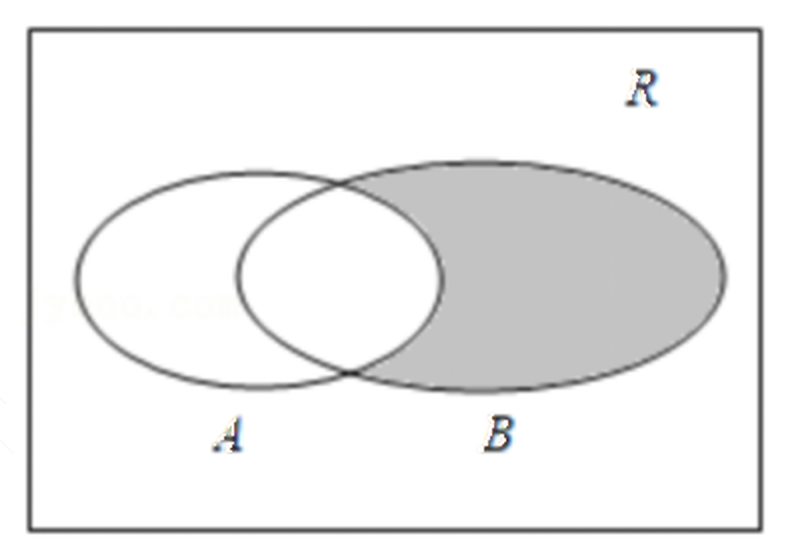
\includegraphics[width=0.36\textwidth]{figures/gao127_q4.png}
\end{center}

\ifanswer
\solbegin
\step{已知 $\R$ 是实数集，集合 $A=\{x\mid 1<x<2\}$, $B=\left\{x\mid 0<x<\frac32\right\}$,}
\step{阴影部分表示的集合是 $\overline A\cap B=\{x\mid 0<x\leqslant1\}$，即 $(0,1]$.}
\solend
\fi

\item 若集合 $\{x\mid (a-1)x^2+3x-2=0\}$ 有且仅有两个子集，则实数 $a$ 的值为\blankline[4.4em].

\ifanswer
\solbegin
\step{由题意得 $\{x\mid (a-1)x^2+3x-2=0\}$ 为单元素集，}
\step{所以 $a-1=0$ 或 $\begin{cases}a-1\neq0\\\triangle=9+8(a-1)=0\end{cases}$，所以 $a=1$ 或 $a=-\frac18$.}
\solend
\fi

\item 已知条件 $\alpha:x\leqslant m$，条件 $\beta:x^2-x\leqslant0$，若 $\alpha$ 是 $\beta$ 的必要条件，则实数 $m$ 的取值范围是为\blankline[4.4em].

\ifanswer
\solbegin
\step{不等式 $x^2-x\leqslant0$ 的解集为 $[0,1]$，}
\step{因为条件 $\alpha:x\leqslant m$，条件 $\beta:x^2-x\leqslant0$，且 $\alpha$ 是 $\beta$ 的必要条件，}
\step{所以集合 $[0,1]$ 是集合 $(-\infty,m]$ 的子集，得 $m\geqslant1$，实数 $m$ 的取值范围是 $[1,+\infty)$.}
\solend
\fi

\item 已知 $\alpha\in\{-2,-1,-\frac12,0,1,2\}$，若幂函数 $y=x^\alpha$ 在 $(0,+\infty)$ 是严格减函数且图像关于 $y$ 轴对称，则 $\alpha=$\blankline[4.4em].

\ifanswer
\solbegin
\step{幂函数 $y=x^\alpha$ 在 $(0,+\infty)$ 是严格减函数，则 $\alpha<0$，且图像关于 $y$ 轴对称，}
\step{则函数为偶函数，故 $\alpha=-2$.}
\solend
\fi

\item 若关于 $x$ 的不等式 $ax^2-3x+2<0$ 的解集不是空集，则实数 $a$ 的取值范围是\blankline[4.4em].

\ifanswer
\solbegin
\step{若 $a>0$，关于 $x$ 的不等式 $ax^2-3x+2<0$ 的解集不空，}
\step{所以一元二次方程 $ax^2-3x+2=0$ 的判别式大于零，}
\step{即 $(-3)^2-8a>0\Rightarrow a<\frac98$，结合 $a>0$ 得 $0<a<\frac98$；}
\step{若 $a\leqslant0$，则关于 $x$ 的不等式 $ax^2-3x+2<0$ 的解集不是空集；}
\step{综上，实数 $a$ 的取值范围是 $\left(-\infty,\frac98\right)$.}
\solend
\fi

\item 设 $\log_{18}2=a$，则 $\log_2 3$ 可用 $a$ 表示为\blankline[4.4em].

\ifanswer
\solbegin
\step{因为 $\log_{18}2=\frac{\log_2 2}{\log_2 18}=\frac1{1+2\log_2 3}=a$，则 $\log_2 3=\frac{1-a}{2a}$.}
\solend
\fi

\item 若关于 $x$ 的不等式 $ax^2+bx+c>0$ 解集为 $\left(-\frac12,3\right)$，则关于 $x$ 的不等式 $cx^2+bx+a<0$ 的解集为\blankline[4.4em].

\ifanswer
\solbegin
\step{由已知得 $a<0$，且 $ax^2+bx+c=a\left(x+\frac12\right)(x-3)$，}
\step{所以 $b=-\frac52 a, c=-\frac32 a$，}
\step{$cx^2+bx+a=-\frac a2(3x-1)(x+2)<0\Leftrightarrow(3x-1)(x+2)<0\Leftrightarrow -2<x<\frac13$，}
\step{故解集为 $\left(-2,\frac13\right)$.}
\solend
\fi

\item 设 $x\in\R$，则方程 $\lvert 2x+3\rvert-\lvert x-2\rvert=\lvert 3x+1\rvert$ 的解集为\blankline[4.4em].

\ifanswer
\solbegin
\step{当 $x\leqslant-\frac32$ 时，原式 $\Leftrightarrow -2x-3+x-2=-3x-1\Leftrightarrow x=2$，不合题意；}
\step{当 $-\frac32<x\leqslant-\frac13$ 时，原式 $\Leftrightarrow 2x+3+x-2=-3x-1\Leftrightarrow x=-\frac13$；}
\step{当 $-\frac13<x\leqslant2$ 时，原式 $\Leftrightarrow 2x+3+x-2=3x+1\Leftrightarrow 1=1$ 即恒成立；}
\step{当 $x>2$ 时，原式 $\Leftrightarrow 2x+3+2-x=3x+1\Leftrightarrow x=2$，不合题意；}
\step{故 $x\in\left[-\frac13,2\right]$.}
\solend
\fi

\item 若关于 $x$ 的不等式 $x^2-4mx+m<0$ 的解集为 $(x_1,x_2)$，若 $x_1>0,x_2>0$，试探究 $x_1+x_2,x_1x_2,x_1^2+x_2^2,\frac1{x_1}+\frac1{x_2}$ 的值，则 $4x_1+x_2$ 的最小值为\blankline[4.4em].

\ifanswer
\solbegin
\step{由题意得方程 $x^2-4mx+m=0$ 有两个相异的正实根 $x_1,x_2$，}
\step{故有 $\begin{cases}\triangle=16m^2-4m>0\\x_1+x_2=4m>0\\x_1\cdot x_2=m>0\end{cases}$，解得 $m>\frac14$，}
\step{则 $x_1^2+x_2^2=(x_1+x_2)^2-2x_1\cdot x_2=16m^2-2m$，$\frac1{x_1}+\frac1{x_2}=\frac{x_1+x_2}{x_1\cdot x_2}=4$，}
\step{则 $4x_1+x_2=\frac14(4x_1+x_2)\left(\frac1{x_1}+\frac1{x_2}\right)=\frac14\left(5+\frac{4x_1}{x_2}+\frac{x_2}{x_1}\right)\geqslant\frac94$，}
\step{当且仅当 $\frac{4x_1}{x_2}=\frac{x_2}{x_1}$ 时，即 $x_2=2x_1$ 时取等号，}
\step{由 $\begin{cases}x_2=2x_1\\\frac1{x_1}+\frac1{x_2}=4\end{cases}$，解得 $\begin{cases}x_1=\frac38\\x_2=\frac34\end{cases}$，于是 $m=x_1\cdot x_2=\frac9{32}\in\left(\frac14,+\infty\right)$，}
\step{即当 $m=\frac9{32}$ 时，$4x_1+x_2$ 取得最小值为 $\frac94$.}
\solend
\fi

\end{enumerate}

\bigsec{二、选择题}

\begin{enumerate}
\setcounter{enumi}{12}

\item 若 $a>0$, $a\neq1$, $M>0$, $N>0$，下列运算正确的是\mbox{（\quad）}

\keepwithprev
A. $\log_a\sqrt[N]{M}=\frac1N\log_a M$\qquad\qquad B. $(\log_a M)^N=N\log_a M$

C. $(\log_a M)\div(\log_a N)=\log_a(M-N)$\qquad\quad D. $\log_a M+\log_a N=\log_a(M+N)$

\ifanswer
\solbegin
\step{对于 $A$，$\log_a\sqrt[N]{M}=\log_a M^{\frac1N}=\frac1N\log_a M$，故 $A$ 正确；}
\step{对于 $B$，$(\log_a M)^N\neq N\log_a M=log_a M^n$，故 $B$ 错误；}
\step{对于 $C$，$(\log_a M)\div(\log_a N)\neq\log_a(M-N)$，故 $C$ 错误；}
\step{对于 $D$，$\log_a M+\log_a N=\log_a MN\neq\log_a(M+N)$，故 $D$ 错误.}
\step{故选 $A$.}
\solend
\fi

\item 下列不等式中正确的是\mbox{（\quad）}

\keepwithprev
A. 若 $a>b$，则 $ac^2>bc^2$\qquad\qquad B. 若 $a<b<0$，则 $a^2<b^2$

C. 若 $1<a<2$ 且 $0<b<3$，则 $1<a+b<5$\qquad D. 若 $\frac1a<1$，则 $a>1$

\ifanswer
\solbegin
\step{$C$ 中 $1+0<a+b<2+3$，即 $1<a+b<5$，正确.}
\step{$A$ 取 $c=0$ 时不成立；$B$ 应为 $a^2>b^2$；$D$ 取 $a=-1$ 时不成立. 故选 $C$.}
\solend
\fi

\item 已知 $y_1=x^3,y_2=x^2$，则下列说法正确的是\mbox{（\quad）}

\keepwithprev
A. $x\in(0,+\infty)$ 时，恒有 $y_1\geqslant y_2$

B. $y_1=x^3$ 与 $y_2=x^2$ 的函数图象仅有唯一交点

C. $x\in(0,1)$ 时，$y_1=x^3$ 图象在 $y_2=x^2$ 图象下方

D. 存在 $x_0\in(1,+\infty)$ 使得 $y_1=y_2$

\ifanswer
\solbegin
\step{$y_1-y_2=x^2(x-1)$，当 $0<x<1$ 时，$y_1<y_2$，故 $C$ 正确，$A$ 错误.}
\step{$y_1=y_2\Leftrightarrow x^2(x-1)=0\Leftrightarrow x=0$ 或 $x=1$，两图象有两个交点，故 $BD$ 错误.}
\step{故选 $C$.}
\solend
\fi

\item 已知非空集合 $A$、$B$ 满足两个条件：(1) $A\cup B=\{1,2,3,4,5,6,7\}$, $A\cap B=\varnothing$；(2) 若 $x\in A$，则 $x+1\in B$，则有序集合对 $(A,B)$ 的个数为\mbox{（\quad）}

\keepwithprev
A. $17$\qquad\qquad B. $18$\qquad\qquad C. $19$\qquad\qquad D. $20$

\ifanswer
\solbegin
\step{当 $A$ 为单元素集合时，有 6 种情况：}
\step{当 $A$ 为双元素集合时，$A=\{1,3\}, A=\{1,4\}, A=\{1,5\}, A=\{1,6\}, A=\{2,4\}$,}
\step{$A=\{2,5\}, A=\{2,6\}, A=\{3,5\}, A=\{3,6\}, A=\{4,6\}$，共 10 种情况；}
\step{当 $A$ 为三元素集合时，$A=\{1,3,5\}, A=\{1,3,6\}, A=\{1,4,6\}, A=\{2,4,6\}$，}
\step{共 4 种情况；}
\step{当 $A$ 为四元素集合时，不成立；}
\step{故有序集合对 $(A,B)$ 的个数为 20，故选 $D$.}
\solend
\fi

\end{enumerate}

\bigsec{三、解答题}

\begin{enumerate}
\setcounter{enumi}{16}

\item 已知 $x,y\in\R$，比较 $x^2+y^2$ 与 $2(2x-y)-5$ 的大小.

\ifanswer
\solbegin
\step{因为 $x^2+y^2-2(2x-y)+5=(x-2)^2+(y+1)^2\geqslant0$，}
\step{所以 $x^2+y^2\geqslant2(2x-y)-5$.}
\solend
\fi

\item 已知集合 $A=\{x\mid x^2+4x=0\}$，$B=\{x\mid x^2+2(a+1)x+a^2-1=0\}$.

(1) 若 $A$ 是 $B$ 的子集，求实数 $a$ 的值；

(2) 若 $B$ 是 $A$ 的子集，求实数 $a$ 的取值范围.

\ifanswer
\solbegin
\step{(1) 因为 $A=\{-4,0\}$，$B=\{x\mid x^2+2(a+1)x+a^2-1=0\}$，又 $A\subseteq B$，}
\step{所以 $A=B$，所以 $\begin{cases}-4+0=-2(a+1)\\-4\times0=a^2-1\end{cases}$，所以 $a=1$；}
\step{(2) 因为 $B$ 是 $A$ 的子集，所以 $B=\varnothing$ 或 $B=\{-4\}$ 或 $B=\{0\}$ 或 $B=\{-4,0\}$，}
\step{① $B=\varnothing$ 时，$\triangle=4(a+1)^2-4(a^2-1)<0$，所以 $a<-1$；}
\step{② $B=\{-4\}$ 时，$\begin{cases}-4+(-4)=-2(a+1)\\-4\times(-4)=a^2-1\end{cases}$，无解；}
\step{③ $B=\{0\}$ 时，$\begin{cases}0+0=-2(a+1)\\0\times0=a^2-1\end{cases}$，所以 $a=-1$；}
\step{④ $B=\{-4,0\}$ 时，由 (1) 得 $a=1$，}
\step{综上，实数 $a$ 的取值范围为 $(-\infty,-1]\cup\{1\}$.}
\solend
\fi

\item 某企业在现有设备下每日生产原先成本 $y$（单位：万元）与日产量 $x$（单位：吨）之间的函数关系式：$y=2x^2+(15-4k)x+120k+8$，近年来各部门都非常重视大气污染防治工作，为了配合环境卫生综合整治，该企业引进了除尘设备，每吨产品的除尘费用为 $k$ 万元，引进除尘设备后，当日产量 $x=1$ 时，总成本（总成本为原先成本和除尘费用之和）为 142 万元.

(1) 求 $k$ 的值；

(2) 求引进除尘设备后日产量为多少时，每吨产品的成本最小，并求出最小值.

\ifanswer
\solbegin
\step{(1) 该企业引进了除尘设备，}
\step{每日生产总成本 $h$（单位：万元）与日产量 $x$（单位：吨）之间的关系为}
\step{$h=2x^2+(15-4k)x+120k+8+kx=2x^2+(15-3k)x+120k+8$，}
\step{当日产量 $x=1$ 时，总成本为 $h=142$ 万元，}
\step{代入得 $2+(15-3k)+120k+8=142\Rightarrow k=1$，}
\step{(2) 由 (1) 得 $h=2x^2+12x+128$，}
\step{所以每吨产品的成本为 $w=\frac{2x^2+12x+128}{x}=2x+\frac{128}{x}+12$}
\step{$\geqslant2\sqrt{2x\cdot\frac{128}{x}}+12=44$，当且仅当 $2x=\frac{128}{x}$，即 $x=8$ 时，取等号，}
\step{所以引进除尘设备后日产量为 8 吨时，每吨产品的成本最小，}
\step{且最小值为 44 万元.}
\solend
\fi

\item 已知集合 $A=\{x\mid \lvert x-a\rvert<2\}$，集合 $B=\left\{x\mid\frac{2x-1}{x+2}<1\right\}$.

(1) 若 $a=2$，求 $A\cup B$；

(2) 若 $A\cap B=A$，求实数 $a$ 的取值范围.

\ifanswer
\solbegin
\step{(1) 若 $a=2$，则 $A=\{x\mid \lvert x-a\rvert<2\}=\{x\mid \lvert x-2\rvert<2\}=\{x\mid 0<x<4\}$，}
\step{由 $\frac{2x-1}{x+2}<1$ 得 $\frac{x-3}{x+2}<0$，即 $(x-3)(x+2)<0$，解得 $-2<x<3$，}
\step{所以 $B=\{x\mid -2<x<3\}$，所以 $A\cup B=\{x\mid -2<x<4\}$；}
\step{(2) 由 (1) 得 $B=\{x\mid -2<x<3\}$，}
\step{$A=\{x\mid \lvert x-a\rvert<2\}=\{x\mid a-2<x<a+2\}$，}
\step{若 $A\cap B=A$，则 $A\subseteq B$，则 $\begin{cases}a-2\geqslant-2\\a+2\leqslant3\end{cases}$，解得 $0\leqslant a\leqslant1$，}
\step{即实数 $a$ 的取值范围为 $[0,1]$.}
\solend
\fi

\item 已知自变量为 $x$ 的函数 $y=\frac{ax+b}{x+a}$，

(1) 若 $a=1$ 且 $b=2$，则函数 $y=\frac{ax+b}{x+a}$ 图像可由幂函数\blankline[4.4em]（写解析式）先沿 $x$ 轴方向\blankline[4.4em]平移\blankline[4.4em]个单位，再沿 $y$ 轴方向向上平移\blankline[4.4em]个单位得到；

(2) 当 $a>0$ 且 $b=-2$ 时不等式 $\frac{ax+b}{x+a}\leqslant\frac{2x^2}{x+a}$ 对 $x>0$ 恒成立，求实数 $a$ 的最大值；

(3) 若 $b=-2$ 且关于 $x$ 的不等式 $x^2\log_2\frac{4(a+1)}a+2x\log_2\frac{2a}{a+1}+\log_2\frac{(a+1)^2}{4a^2}\leqslant0$ 解集是单元素集，求出 $a$ 值，并求出函数 $y=\frac{ax-2}{x+a}$ 的对称中心.

\ifanswer
\solbegin
\step{(1) 已知自变量为 $x$ 的函数 $y=\frac{ax+b}{x+a}$，}
\step{当 $a=1$ 且 $b=2$ 时，$y=\frac{x+2}{x+1}=\frac{x+1+1}{x+1}=1+\frac1{x+1}$，}
\step{由幂函数 $y=\frac1x$，先沿 $x$ 轴方向向左平移一个单位，}
\step{再沿 $y$ 轴方向向上平移一个单位得到；}
\step{(2) 当 $a>0$ 且 $b=-2$ 时不等式 $\frac{ax+b}{x+a}\leqslant\frac{2x^2}{x+a}$ 即 $\frac{ax-2}{x+a}\leqslant\frac{2x^2}{x+a}$ 对 $x>0$ 恒成立，}
\step{因为 $a>0$ 且 $x>0$，所以 $x+a>0$，所以等价于 $ax-2\leqslant2x^2$ 对 $x>0$ 恒成立，}
\step{即 $2x^2-ax+2\geqslant0$ 对 $x>0$ 恒成立，}
\step{因为函数 $g(x)=2x^2-ax+2$ 的对称轴 $x=\frac a4>0$，且 $g(0)=2>0$，}
\step{则 $\begin{cases}\triangle=(-a)^2-4\times2\times2\leqslant0\\a>0\end{cases}$，解得 $0<a\leqslant4$，所以 $a$ 的最大值为 4；}
\step{(3) 关于 $x$ 的不等式 $x^2\log_2\frac{4(a+1)}a+2x\log_2\frac{2a}{a+1}+\log_2\frac{(a+1)^2}{4a^2}\leqslant0$ 解集}
\step{是单元素集，由 $\frac{4(a+1)}a>0$，则 $a>0$ 或 $a<-1$，}
\step{若 $\log_2\frac{4(a+1)}a=0$，则 $\frac{4(a+1)}a=1$，解得 $a=-\frac43$，}
\step{此时不等式为 $6x-6\leqslant0$，解得 $x\leqslant1$，不符合题意，}
\step{若 $\log_2\frac{4(a+1)}a>0$，即 $\frac{4(a+1)}a>1$，解得 $a>0$ 或 $a<-\frac43$，}
\step{则 $\triangle=\left(2\log_2\frac{2a}{a+1}\right)^2-4\log_2\frac{4(a+1)}a\cdot\log_2\frac{(a+1)^2}{4a^2}=0$，}
\step{令 $\log_2\frac{2a}{a+1}=t$，则 $t^2-(3-t)(-2t)=0$，解得 $t=0$ 或 $t=6$，}
\step{当 $\log_2\frac{2a}{a+1}=0$，解得 $a=1$，$\log_2\frac{2a}{a+1}=6$，解得 $a=-\frac{32}{31}$(舍去)，所以 $a=1$，}
\step{则函数 $y=\frac{ax-2}{x+a}$ 即为 $y=\frac{x-2}{x+1}=\frac{x+1-3}{x+1}=1+\frac{-3}{x+1}$，}
\step{对称中心为 $(-1,1)$.}
\solend
\fi

\end{enumerate}

\end{document}
"
% 紧凑版：xelatex "\def\iscompact{1}% 高一127_南汇一中_期中.tex
%   —— 高一上数学“2026-2027 年南汇一中高一上期中”（试卷版/答案版）
% 试卷版：xelatex 高一127_南汇一中_期中.tex
% 答案版：xelatex "\def\isanswer{1}\input{高一127_南汇一中_期中.tex}"
% 紧凑版：xelatex "\def\iscompact{1}\input{高一127_南汇一中_期中.tex}"
%
% 原始材料：微信公众号“魔都数学加油站”文章，作者破晓，2026-11-11 18:35 发布；
% 连载“27学年高一127”，原文标题“27学年高一127——2026-2027年上海市南汇一中高一上期中”；
% 原文链接：https://mp.weixin.qq.com/s/nozIwRgeWSKPCPSiqfCm2Q。
% 正文为 9 张 PNG 页（01、02、03、09 为 2560×3620，04、05、06、07、08 为 4762×6735），
% 题目下印有【解析】，为讲评版。题目、解析均据原图转录；
% 卷面粉红色水印“魔都数学加油站”及公众号页脚未录入。全卷仅第 4 题一幅插图。
% 第 09 页只有一行“对称中心为(-1,1).”及水印，是第 08 页末行的续尾页。
%
% 卷首标题：原卷印作“2026-2027 年南汇一中高一上期中”（公众号标题中的“上海市”
% 卷面标题行没有，本稿照卷面），年份区间按全稿惯例排 en dash；原卷未印副标题，
% 本卷为期中卷、跨三章，按题目内容标为“集合与常用逻辑用语、不等式、函数”
% （第 4/5/6/16/18/20 题为集合与常用逻辑用语，第 8/10/11/12/14/17 题为不等式，
% 第 3/7/9/13/15/19/21 题为函数；与 106、125 同为期中复习卷，口径相同）。
%
% 与原卷的排版差异：
%   ① 原文从第 3 题起，填空题编号为 3—12、选择题为 13—16、解答题为 17—21，本稿保留原题号；
%   ② 原卷每题下直接印【解析】，本稿按全稿惯例置于答案版；四道选择题答案均在解析末句
%      “故选 …”，括号内留空、不另提 \ans{}；全卷无只印【答案】或括号内答案的题；
%   ③ 原卷未印副标题，本稿按“知识模块”口径补出；
%   ④ 原卷填空横线按全稿惯例排为 \blankline[4.4em]；选择题括号排 \mbox{（\quad）}、
%      选项段前按惯例加 \keepwithprev；解答题不留作答区（原卷为讲评版，与 109—125 同）；
%      第 21 题 (1) 的四处填空横线亦排 \blankline[4.4em]；
%   ⑤ 原卷数集排斜体 $R$，按全稿惯例改 \R；绝对值排 \lvert…\rvert，集合描述竖线排 \mid；
%      补集记号照原卷上划线排 \overline{A}；不等号一律 \leqslant / \geqslant；
%   ⑥ 第 4 题插图原在题干右侧，本稿按全稿惯例移至题干之后居中排（取原卷截图、
%      去粉色水印后 2× LANCZOS 放大，存 figures/gao127_q4.png），三版都出；
%      并在该题 \item 前加 \needvspace{} 守卫，把题干与插图整块推走；
%   ⑦ 原卷子题编号 (1)(2)(3) 与括号按全稿惯例排；“（单位：万元）”“（写解析式）”
%      用全角括号，第 21 题 (3) 解析“(舍去)”用半角括号，均照录；
%   ⑧ 第 09 页仅一行“对称中心为(-1,1).”为第 08 页末行之续尾，本稿按原卷印刷行
%      另起一条 \step，置于答案版最后一题解析之末。
%
% 子集符号：第 18 题 (1) 解析 $A\subseteq B$、第 20 题 (2) 解析 $A\subseteq B$ 均印有
%   下划线，照录 \subseteq；全卷无 \subset。回原图放大逐处确认。
%
% 判别式字形：本卷 5 处判别式（第 5 题解析 cases 内 $\triangle=9+8(a-1)=0$、
%   第 12 题解析 cases 内 $\triangle=16m^2-4m>0$、第 18 题① $\triangle=4(a+1)^2-4(a^2-1)<0$、
%   第 21 题 (2) cases 内 $\triangle=(-a)^2-4\times2\times2\leqslant0$、
%   第 21 题 (3) $\triangle=\left(2\log_2\frac{2a}{a+1}\right)^2-\cdots=0$）均排等边扁三角，
%   照录 \triangle；逐处回原图全分辨率放大确认，无高三角 $\Delta$（与 高一26 排 $\Delta$ 不同）。
%
% 原卷存疑照录：
%   第 6 题题干作“则实数 $m$ 的取值范围是为____”（“是为”叠用，疑衍一字），照录；
%   第 12 题题干“试探究 $x_1+x_2, x_1x_2, x_1^2+x_2^2, \frac1{x_1}+\frac1{x_2}$ 的值，
%     则 $4x_1+x_2$ 的最小值为____”与后文衔接突兀，照录；
%   第 13 题解析 B 作“$(\log_a M)^N\neq N\log_a M=log_a M^n$”，后一 log 为斜体、
%     指数作小写 $n$，与前式 $N\log_a M$ 及题干 $N$ 不一致，照录；
%   第 13 题解析 A、B、C 三步句末用“；”，D 步句末用“.”，标点不一致，照录；
%   第 15 题解析“故 $BD$ 错误.”两选项字母连写、无顿号，照录；
%   第 7 题题干及解析用“图像”，第 15 题 B、C 及解析用“图象”，全卷两种写法混用，照录未统一；
%   第 21 题 (3) 题干“求出 $a$ 值”（通常作“求出 $a$ 的值”），照录；
%   第 21 题 (3) 解析“解得 $a=1$，$\log_2\frac{2a}{a+1}=6$，解得 $a=-\frac{32}{31}$(舍去)，
%     所以 $a=1$”两个“解得”并列、且舍去值用半角括号，照录；
%   第 09 页“对称中心为(-1,1).”用半角括号与半角句点，照录；
%   第 8 题解析“若 $a\leqslant0$，则关于 $x$ 的不等式 $ax^2-3x+2<0$ 的解集不是空集；”
%     未给理由直接断言，照录；
%   第 18 题 (1) 由 $A\subseteq B$ 直接得 $A=B$，照录。
%
% 行数核对：逐题数 \step 条数，合计 95 条（Q3：1；Q4：2；Q5：2；Q6：3；Q7：2；
% Q8：5；Q9：1；Q10：4；Q11：5；Q12：7；Q13：5；Q14：2；Q15：3；Q16：7；
% Q17：2；Q18：8；Q19：10；Q20：7；Q21：19），与原卷印刷行逐题相等
% （cases 块作一个印刷行计；Q21 第 19 行为第 09 页续尾）。全卷 19 题均印【解析】，
% 无只印【答案】或括号内答案的题，故 \ans{} 为 0；四道选择题括号内留空、不另提 \ans{}。
%
\documentclass[a4paper,11pt]{article}
\usepackage{common}

\begin{document}

\examtitlest[3]{2026--2027 年南汇一中高一上期中}{集合与常用逻辑用语、不等式、函数}

\bigsec{一、填空题}

\begin{enumerate}
\setcounter{enumi}{2}

\item 把 $\sqrt[4]{a\sqrt a}(a>0)$ 化成有理数指数幂的形式为\blankline[4.4em].

\ifanswer
\solbegin
\step{$\sqrt[4]{a\sqrt a}=(a\cdot a^{\frac12})^{\frac14}=a^{\frac38}$.}
\solend
\fi

\needvspace{6.5cm}
\item 已知集合 $A=\{x\mid 1<x<2\}$, $B=\left\{x\mid 0<x<\frac32\right\}$, 则如图阴影部分表示的集合是\blankline[4.4em].

\begin{center}
% 图取原卷截图（第 1 页题干右侧）、去水印后 2× LANCZOS 放大，本稿移至题干之后
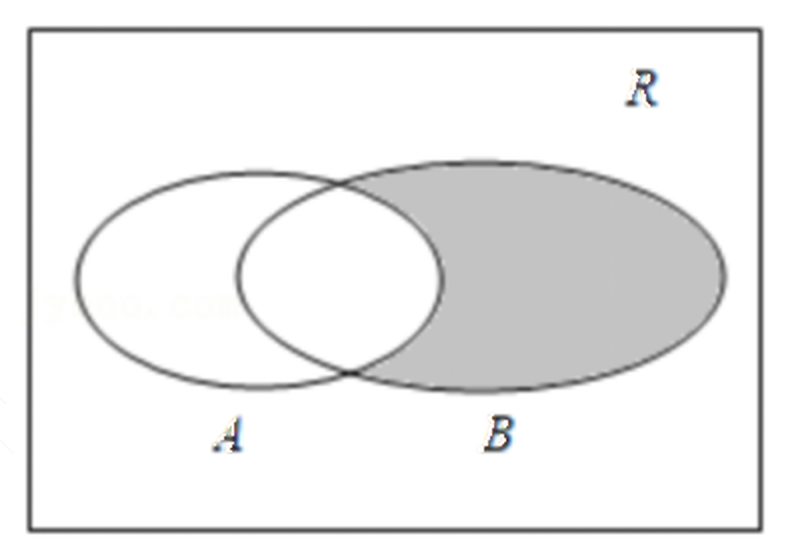
\includegraphics[width=0.36\textwidth]{figures/gao127_q4.png}
\end{center}

\ifanswer
\solbegin
\step{已知 $\R$ 是实数集，集合 $A=\{x\mid 1<x<2\}$, $B=\left\{x\mid 0<x<\frac32\right\}$,}
\step{阴影部分表示的集合是 $\overline A\cap B=\{x\mid 0<x\leqslant1\}$，即 $(0,1]$.}
\solend
\fi

\item 若集合 $\{x\mid (a-1)x^2+3x-2=0\}$ 有且仅有两个子集，则实数 $a$ 的值为\blankline[4.4em].

\ifanswer
\solbegin
\step{由题意得 $\{x\mid (a-1)x^2+3x-2=0\}$ 为单元素集，}
\step{所以 $a-1=0$ 或 $\begin{cases}a-1\neq0\\\triangle=9+8(a-1)=0\end{cases}$，所以 $a=1$ 或 $a=-\frac18$.}
\solend
\fi

\item 已知条件 $\alpha:x\leqslant m$，条件 $\beta:x^2-x\leqslant0$，若 $\alpha$ 是 $\beta$ 的必要条件，则实数 $m$ 的取值范围是为\blankline[4.4em].

\ifanswer
\solbegin
\step{不等式 $x^2-x\leqslant0$ 的解集为 $[0,1]$，}
\step{因为条件 $\alpha:x\leqslant m$，条件 $\beta:x^2-x\leqslant0$，且 $\alpha$ 是 $\beta$ 的必要条件，}
\step{所以集合 $[0,1]$ 是集合 $(-\infty,m]$ 的子集，得 $m\geqslant1$，实数 $m$ 的取值范围是 $[1,+\infty)$.}
\solend
\fi

\item 已知 $\alpha\in\{-2,-1,-\frac12,0,1,2\}$，若幂函数 $y=x^\alpha$ 在 $(0,+\infty)$ 是严格减函数且图像关于 $y$ 轴对称，则 $\alpha=$\blankline[4.4em].

\ifanswer
\solbegin
\step{幂函数 $y=x^\alpha$ 在 $(0,+\infty)$ 是严格减函数，则 $\alpha<0$，且图像关于 $y$ 轴对称，}
\step{则函数为偶函数，故 $\alpha=-2$.}
\solend
\fi

\item 若关于 $x$ 的不等式 $ax^2-3x+2<0$ 的解集不是空集，则实数 $a$ 的取值范围是\blankline[4.4em].

\ifanswer
\solbegin
\step{若 $a>0$，关于 $x$ 的不等式 $ax^2-3x+2<0$ 的解集不空，}
\step{所以一元二次方程 $ax^2-3x+2=0$ 的判别式大于零，}
\step{即 $(-3)^2-8a>0\Rightarrow a<\frac98$，结合 $a>0$ 得 $0<a<\frac98$；}
\step{若 $a\leqslant0$，则关于 $x$ 的不等式 $ax^2-3x+2<0$ 的解集不是空集；}
\step{综上，实数 $a$ 的取值范围是 $\left(-\infty,\frac98\right)$.}
\solend
\fi

\item 设 $\log_{18}2=a$，则 $\log_2 3$ 可用 $a$ 表示为\blankline[4.4em].

\ifanswer
\solbegin
\step{因为 $\log_{18}2=\frac{\log_2 2}{\log_2 18}=\frac1{1+2\log_2 3}=a$，则 $\log_2 3=\frac{1-a}{2a}$.}
\solend
\fi

\item 若关于 $x$ 的不等式 $ax^2+bx+c>0$ 解集为 $\left(-\frac12,3\right)$，则关于 $x$ 的不等式 $cx^2+bx+a<0$ 的解集为\blankline[4.4em].

\ifanswer
\solbegin
\step{由已知得 $a<0$，且 $ax^2+bx+c=a\left(x+\frac12\right)(x-3)$，}
\step{所以 $b=-\frac52 a, c=-\frac32 a$，}
\step{$cx^2+bx+a=-\frac a2(3x-1)(x+2)<0\Leftrightarrow(3x-1)(x+2)<0\Leftrightarrow -2<x<\frac13$，}
\step{故解集为 $\left(-2,\frac13\right)$.}
\solend
\fi

\item 设 $x\in\R$，则方程 $\lvert 2x+3\rvert-\lvert x-2\rvert=\lvert 3x+1\rvert$ 的解集为\blankline[4.4em].

\ifanswer
\solbegin
\step{当 $x\leqslant-\frac32$ 时，原式 $\Leftrightarrow -2x-3+x-2=-3x-1\Leftrightarrow x=2$，不合题意；}
\step{当 $-\frac32<x\leqslant-\frac13$ 时，原式 $\Leftrightarrow 2x+3+x-2=-3x-1\Leftrightarrow x=-\frac13$；}
\step{当 $-\frac13<x\leqslant2$ 时，原式 $\Leftrightarrow 2x+3+x-2=3x+1\Leftrightarrow 1=1$ 即恒成立；}
\step{当 $x>2$ 时，原式 $\Leftrightarrow 2x+3+2-x=3x+1\Leftrightarrow x=2$，不合题意；}
\step{故 $x\in\left[-\frac13,2\right]$.}
\solend
\fi

\item 若关于 $x$ 的不等式 $x^2-4mx+m<0$ 的解集为 $(x_1,x_2)$，若 $x_1>0,x_2>0$，试探究 $x_1+x_2,x_1x_2,x_1^2+x_2^2,\frac1{x_1}+\frac1{x_2}$ 的值，则 $4x_1+x_2$ 的最小值为\blankline[4.4em].

\ifanswer
\solbegin
\step{由题意得方程 $x^2-4mx+m=0$ 有两个相异的正实根 $x_1,x_2$，}
\step{故有 $\begin{cases}\triangle=16m^2-4m>0\\x_1+x_2=4m>0\\x_1\cdot x_2=m>0\end{cases}$，解得 $m>\frac14$，}
\step{则 $x_1^2+x_2^2=(x_1+x_2)^2-2x_1\cdot x_2=16m^2-2m$，$\frac1{x_1}+\frac1{x_2}=\frac{x_1+x_2}{x_1\cdot x_2}=4$，}
\step{则 $4x_1+x_2=\frac14(4x_1+x_2)\left(\frac1{x_1}+\frac1{x_2}\right)=\frac14\left(5+\frac{4x_1}{x_2}+\frac{x_2}{x_1}\right)\geqslant\frac94$，}
\step{当且仅当 $\frac{4x_1}{x_2}=\frac{x_2}{x_1}$ 时，即 $x_2=2x_1$ 时取等号，}
\step{由 $\begin{cases}x_2=2x_1\\\frac1{x_1}+\frac1{x_2}=4\end{cases}$，解得 $\begin{cases}x_1=\frac38\\x_2=\frac34\end{cases}$，于是 $m=x_1\cdot x_2=\frac9{32}\in\left(\frac14,+\infty\right)$，}
\step{即当 $m=\frac9{32}$ 时，$4x_1+x_2$ 取得最小值为 $\frac94$.}
\solend
\fi

\end{enumerate}

\bigsec{二、选择题}

\begin{enumerate}
\setcounter{enumi}{12}

\item 若 $a>0$, $a\neq1$, $M>0$, $N>0$，下列运算正确的是\mbox{（\quad）}

\keepwithprev
A. $\log_a\sqrt[N]{M}=\frac1N\log_a M$\qquad\qquad B. $(\log_a M)^N=N\log_a M$

C. $(\log_a M)\div(\log_a N)=\log_a(M-N)$\qquad\quad D. $\log_a M+\log_a N=\log_a(M+N)$

\ifanswer
\solbegin
\step{对于 $A$，$\log_a\sqrt[N]{M}=\log_a M^{\frac1N}=\frac1N\log_a M$，故 $A$ 正确；}
\step{对于 $B$，$(\log_a M)^N\neq N\log_a M=log_a M^n$，故 $B$ 错误；}
\step{对于 $C$，$(\log_a M)\div(\log_a N)\neq\log_a(M-N)$，故 $C$ 错误；}
\step{对于 $D$，$\log_a M+\log_a N=\log_a MN\neq\log_a(M+N)$，故 $D$ 错误.}
\step{故选 $A$.}
\solend
\fi

\item 下列不等式中正确的是\mbox{（\quad）}

\keepwithprev
A. 若 $a>b$，则 $ac^2>bc^2$\qquad\qquad B. 若 $a<b<0$，则 $a^2<b^2$

C. 若 $1<a<2$ 且 $0<b<3$，则 $1<a+b<5$\qquad D. 若 $\frac1a<1$，则 $a>1$

\ifanswer
\solbegin
\step{$C$ 中 $1+0<a+b<2+3$，即 $1<a+b<5$，正确.}
\step{$A$ 取 $c=0$ 时不成立；$B$ 应为 $a^2>b^2$；$D$ 取 $a=-1$ 时不成立. 故选 $C$.}
\solend
\fi

\item 已知 $y_1=x^3,y_2=x^2$，则下列说法正确的是\mbox{（\quad）}

\keepwithprev
A. $x\in(0,+\infty)$ 时，恒有 $y_1\geqslant y_2$

B. $y_1=x^3$ 与 $y_2=x^2$ 的函数图象仅有唯一交点

C. $x\in(0,1)$ 时，$y_1=x^3$ 图象在 $y_2=x^2$ 图象下方

D. 存在 $x_0\in(1,+\infty)$ 使得 $y_1=y_2$

\ifanswer
\solbegin
\step{$y_1-y_2=x^2(x-1)$，当 $0<x<1$ 时，$y_1<y_2$，故 $C$ 正确，$A$ 错误.}
\step{$y_1=y_2\Leftrightarrow x^2(x-1)=0\Leftrightarrow x=0$ 或 $x=1$，两图象有两个交点，故 $BD$ 错误.}
\step{故选 $C$.}
\solend
\fi

\item 已知非空集合 $A$、$B$ 满足两个条件：(1) $A\cup B=\{1,2,3,4,5,6,7\}$, $A\cap B=\varnothing$；(2) 若 $x\in A$，则 $x+1\in B$，则有序集合对 $(A,B)$ 的个数为\mbox{（\quad）}

\keepwithprev
A. $17$\qquad\qquad B. $18$\qquad\qquad C. $19$\qquad\qquad D. $20$

\ifanswer
\solbegin
\step{当 $A$ 为单元素集合时，有 6 种情况：}
\step{当 $A$ 为双元素集合时，$A=\{1,3\}, A=\{1,4\}, A=\{1,5\}, A=\{1,6\}, A=\{2,4\}$,}
\step{$A=\{2,5\}, A=\{2,6\}, A=\{3,5\}, A=\{3,6\}, A=\{4,6\}$，共 10 种情况；}
\step{当 $A$ 为三元素集合时，$A=\{1,3,5\}, A=\{1,3,6\}, A=\{1,4,6\}, A=\{2,4,6\}$，}
\step{共 4 种情况；}
\step{当 $A$ 为四元素集合时，不成立；}
\step{故有序集合对 $(A,B)$ 的个数为 20，故选 $D$.}
\solend
\fi

\end{enumerate}

\bigsec{三、解答题}

\begin{enumerate}
\setcounter{enumi}{16}

\item 已知 $x,y\in\R$，比较 $x^2+y^2$ 与 $2(2x-y)-5$ 的大小.

\ifanswer
\solbegin
\step{因为 $x^2+y^2-2(2x-y)+5=(x-2)^2+(y+1)^2\geqslant0$，}
\step{所以 $x^2+y^2\geqslant2(2x-y)-5$.}
\solend
\fi

\item 已知集合 $A=\{x\mid x^2+4x=0\}$，$B=\{x\mid x^2+2(a+1)x+a^2-1=0\}$.

(1) 若 $A$ 是 $B$ 的子集，求实数 $a$ 的值；

(2) 若 $B$ 是 $A$ 的子集，求实数 $a$ 的取值范围.

\ifanswer
\solbegin
\step{(1) 因为 $A=\{-4,0\}$，$B=\{x\mid x^2+2(a+1)x+a^2-1=0\}$，又 $A\subseteq B$，}
\step{所以 $A=B$，所以 $\begin{cases}-4+0=-2(a+1)\\-4\times0=a^2-1\end{cases}$，所以 $a=1$；}
\step{(2) 因为 $B$ 是 $A$ 的子集，所以 $B=\varnothing$ 或 $B=\{-4\}$ 或 $B=\{0\}$ 或 $B=\{-4,0\}$，}
\step{① $B=\varnothing$ 时，$\triangle=4(a+1)^2-4(a^2-1)<0$，所以 $a<-1$；}
\step{② $B=\{-4\}$ 时，$\begin{cases}-4+(-4)=-2(a+1)\\-4\times(-4)=a^2-1\end{cases}$，无解；}
\step{③ $B=\{0\}$ 时，$\begin{cases}0+0=-2(a+1)\\0\times0=a^2-1\end{cases}$，所以 $a=-1$；}
\step{④ $B=\{-4,0\}$ 时，由 (1) 得 $a=1$，}
\step{综上，实数 $a$ 的取值范围为 $(-\infty,-1]\cup\{1\}$.}
\solend
\fi

\item 某企业在现有设备下每日生产原先成本 $y$（单位：万元）与日产量 $x$（单位：吨）之间的函数关系式：$y=2x^2+(15-4k)x+120k+8$，近年来各部门都非常重视大气污染防治工作，为了配合环境卫生综合整治，该企业引进了除尘设备，每吨产品的除尘费用为 $k$ 万元，引进除尘设备后，当日产量 $x=1$ 时，总成本（总成本为原先成本和除尘费用之和）为 142 万元.

(1) 求 $k$ 的值；

(2) 求引进除尘设备后日产量为多少时，每吨产品的成本最小，并求出最小值.

\ifanswer
\solbegin
\step{(1) 该企业引进了除尘设备，}
\step{每日生产总成本 $h$（单位：万元）与日产量 $x$（单位：吨）之间的关系为}
\step{$h=2x^2+(15-4k)x+120k+8+kx=2x^2+(15-3k)x+120k+8$，}
\step{当日产量 $x=1$ 时，总成本为 $h=142$ 万元，}
\step{代入得 $2+(15-3k)+120k+8=142\Rightarrow k=1$，}
\step{(2) 由 (1) 得 $h=2x^2+12x+128$，}
\step{所以每吨产品的成本为 $w=\frac{2x^2+12x+128}{x}=2x+\frac{128}{x}+12$}
\step{$\geqslant2\sqrt{2x\cdot\frac{128}{x}}+12=44$，当且仅当 $2x=\frac{128}{x}$，即 $x=8$ 时，取等号，}
\step{所以引进除尘设备后日产量为 8 吨时，每吨产品的成本最小，}
\step{且最小值为 44 万元.}
\solend
\fi

\item 已知集合 $A=\{x\mid \lvert x-a\rvert<2\}$，集合 $B=\left\{x\mid\frac{2x-1}{x+2}<1\right\}$.

(1) 若 $a=2$，求 $A\cup B$；

(2) 若 $A\cap B=A$，求实数 $a$ 的取值范围.

\ifanswer
\solbegin
\step{(1) 若 $a=2$，则 $A=\{x\mid \lvert x-a\rvert<2\}=\{x\mid \lvert x-2\rvert<2\}=\{x\mid 0<x<4\}$，}
\step{由 $\frac{2x-1}{x+2}<1$ 得 $\frac{x-3}{x+2}<0$，即 $(x-3)(x+2)<0$，解得 $-2<x<3$，}
\step{所以 $B=\{x\mid -2<x<3\}$，所以 $A\cup B=\{x\mid -2<x<4\}$；}
\step{(2) 由 (1) 得 $B=\{x\mid -2<x<3\}$，}
\step{$A=\{x\mid \lvert x-a\rvert<2\}=\{x\mid a-2<x<a+2\}$，}
\step{若 $A\cap B=A$，则 $A\subseteq B$，则 $\begin{cases}a-2\geqslant-2\\a+2\leqslant3\end{cases}$，解得 $0\leqslant a\leqslant1$，}
\step{即实数 $a$ 的取值范围为 $[0,1]$.}
\solend
\fi

\item 已知自变量为 $x$ 的函数 $y=\frac{ax+b}{x+a}$，

(1) 若 $a=1$ 且 $b=2$，则函数 $y=\frac{ax+b}{x+a}$ 图像可由幂函数\blankline[4.4em]（写解析式）先沿 $x$ 轴方向\blankline[4.4em]平移\blankline[4.4em]个单位，再沿 $y$ 轴方向向上平移\blankline[4.4em]个单位得到；

(2) 当 $a>0$ 且 $b=-2$ 时不等式 $\frac{ax+b}{x+a}\leqslant\frac{2x^2}{x+a}$ 对 $x>0$ 恒成立，求实数 $a$ 的最大值；

(3) 若 $b=-2$ 且关于 $x$ 的不等式 $x^2\log_2\frac{4(a+1)}a+2x\log_2\frac{2a}{a+1}+\log_2\frac{(a+1)^2}{4a^2}\leqslant0$ 解集是单元素集，求出 $a$ 值，并求出函数 $y=\frac{ax-2}{x+a}$ 的对称中心.

\ifanswer
\solbegin
\step{(1) 已知自变量为 $x$ 的函数 $y=\frac{ax+b}{x+a}$，}
\step{当 $a=1$ 且 $b=2$ 时，$y=\frac{x+2}{x+1}=\frac{x+1+1}{x+1}=1+\frac1{x+1}$，}
\step{由幂函数 $y=\frac1x$，先沿 $x$ 轴方向向左平移一个单位，}
\step{再沿 $y$ 轴方向向上平移一个单位得到；}
\step{(2) 当 $a>0$ 且 $b=-2$ 时不等式 $\frac{ax+b}{x+a}\leqslant\frac{2x^2}{x+a}$ 即 $\frac{ax-2}{x+a}\leqslant\frac{2x^2}{x+a}$ 对 $x>0$ 恒成立，}
\step{因为 $a>0$ 且 $x>0$，所以 $x+a>0$，所以等价于 $ax-2\leqslant2x^2$ 对 $x>0$ 恒成立，}
\step{即 $2x^2-ax+2\geqslant0$ 对 $x>0$ 恒成立，}
\step{因为函数 $g(x)=2x^2-ax+2$ 的对称轴 $x=\frac a4>0$，且 $g(0)=2>0$，}
\step{则 $\begin{cases}\triangle=(-a)^2-4\times2\times2\leqslant0\\a>0\end{cases}$，解得 $0<a\leqslant4$，所以 $a$ 的最大值为 4；}
\step{(3) 关于 $x$ 的不等式 $x^2\log_2\frac{4(a+1)}a+2x\log_2\frac{2a}{a+1}+\log_2\frac{(a+1)^2}{4a^2}\leqslant0$ 解集}
\step{是单元素集，由 $\frac{4(a+1)}a>0$，则 $a>0$ 或 $a<-1$，}
\step{若 $\log_2\frac{4(a+1)}a=0$，则 $\frac{4(a+1)}a=1$，解得 $a=-\frac43$，}
\step{此时不等式为 $6x-6\leqslant0$，解得 $x\leqslant1$，不符合题意，}
\step{若 $\log_2\frac{4(a+1)}a>0$，即 $\frac{4(a+1)}a>1$，解得 $a>0$ 或 $a<-\frac43$，}
\step{则 $\triangle=\left(2\log_2\frac{2a}{a+1}\right)^2-4\log_2\frac{4(a+1)}a\cdot\log_2\frac{(a+1)^2}{4a^2}=0$，}
\step{令 $\log_2\frac{2a}{a+1}=t$，则 $t^2-(3-t)(-2t)=0$，解得 $t=0$ 或 $t=6$，}
\step{当 $\log_2\frac{2a}{a+1}=0$，解得 $a=1$，$\log_2\frac{2a}{a+1}=6$，解得 $a=-\frac{32}{31}$(舍去)，所以 $a=1$，}
\step{则函数 $y=\frac{ax-2}{x+a}$ 即为 $y=\frac{x-2}{x+1}=\frac{x+1-3}{x+1}=1+\frac{-3}{x+1}$，}
\step{对称中心为 $(-1,1)$.}
\solend
\fi

\end{enumerate}

\end{document}
"
%
% 原始材料：微信公众号“魔都数学加油站”文章，作者破晓，2026-11-11 18:35 发布；
% 连载“27学年高一127”，原文标题“27学年高一127——2026-2027年上海市南汇一中高一上期中”；
% 原文链接：https://mp.weixin.qq.com/s/nozIwRgeWSKPCPSiqfCm2Q。
% 正文为 9 张 PNG 页（01、02、03、09 为 2560×3620，04、05、06、07、08 为 4762×6735），
% 题目下印有【解析】，为讲评版。题目、解析均据原图转录；
% 卷面粉红色水印“魔都数学加油站”及公众号页脚未录入。全卷仅第 4 题一幅插图。
% 第 09 页只有一行“对称中心为(-1,1).”及水印，是第 08 页末行的续尾页。
%
% 卷首标题：原卷印作“2026-2027 年南汇一中高一上期中”（公众号标题中的“上海市”
% 卷面标题行没有，本稿照卷面），年份区间按全稿惯例排 en dash；原卷未印副标题，
% 本卷为期中卷、跨三章，按题目内容标为“集合与常用逻辑用语、不等式、函数”
% （第 4/5/6/16/18/20 题为集合与常用逻辑用语，第 8/10/11/12/14/17 题为不等式，
% 第 3/7/9/13/15/19/21 题为函数；与 106、125 同为期中复习卷，口径相同）。
%
% 与原卷的排版差异：
%   ① 原文从第 3 题起，填空题编号为 3—12、选择题为 13—16、解答题为 17—21，本稿保留原题号；
%   ② 原卷每题下直接印【解析】，本稿按全稿惯例置于答案版；四道选择题答案均在解析末句
%      “故选 …”，括号内留空、不另提 \ans{}；全卷无只印【答案】或括号内答案的题；
%   ③ 原卷未印副标题，本稿按“知识模块”口径补出；
%   ④ 原卷填空横线按全稿惯例排为 \blankline[4.4em]；选择题括号排 \mbox{（\quad）}、
%      选项段前按惯例加 \keepwithprev；解答题不留作答区（原卷为讲评版，与 109—125 同）；
%      第 21 题 (1) 的四处填空横线亦排 \blankline[4.4em]；
%   ⑤ 原卷数集排斜体 $R$，按全稿惯例改 \R；绝对值排 \lvert…\rvert，集合描述竖线排 \mid；
%      补集记号照原卷上划线排 \overline{A}；不等号一律 \leqslant / \geqslant；
%   ⑥ 第 4 题插图原在题干右侧，本稿按全稿惯例移至题干之后居中排（取原卷截图、
%      去粉色水印后 2× LANCZOS 放大，存 figures/gao127_q4.png），三版都出；
%      并在该题 \item 前加 \needvspace{} 守卫，把题干与插图整块推走；
%   ⑦ 原卷子题编号 (1)(2)(3) 与括号按全稿惯例排；“（单位：万元）”“（写解析式）”
%      用全角括号，第 21 题 (3) 解析“(舍去)”用半角括号，均照录；
%   ⑧ 第 09 页仅一行“对称中心为(-1,1).”为第 08 页末行之续尾，本稿按原卷印刷行
%      另起一条 \step，置于答案版最后一题解析之末。
%
% 子集符号：第 18 题 (1) 解析 $A\subseteq B$、第 20 题 (2) 解析 $A\subseteq B$ 均印有
%   下划线，照录 \subseteq；全卷无 \subset。回原图放大逐处确认。
%
% 判别式字形：本卷 5 处判别式（第 5 题解析 cases 内 $\triangle=9+8(a-1)=0$、
%   第 12 题解析 cases 内 $\triangle=16m^2-4m>0$、第 18 题① $\triangle=4(a+1)^2-4(a^2-1)<0$、
%   第 21 题 (2) cases 内 $\triangle=(-a)^2-4\times2\times2\leqslant0$、
%   第 21 题 (3) $\triangle=\left(2\log_2\frac{2a}{a+1}\right)^2-\cdots=0$）均排等边扁三角，
%   照录 \triangle；逐处回原图全分辨率放大确认，无高三角 $\Delta$（与 高一26 排 $\Delta$ 不同）。
%
% 原卷存疑照录：
%   第 6 题题干作“则实数 $m$ 的取值范围是为____”（“是为”叠用，疑衍一字），照录；
%   第 12 题题干“试探究 $x_1+x_2, x_1x_2, x_1^2+x_2^2, \frac1{x_1}+\frac1{x_2}$ 的值，
%     则 $4x_1+x_2$ 的最小值为____”与后文衔接突兀，照录；
%   第 13 题解析 B 作“$(\log_a M)^N\neq N\log_a M=log_a M^n$”，后一 log 为斜体、
%     指数作小写 $n$，与前式 $N\log_a M$ 及题干 $N$ 不一致，照录；
%   第 13 题解析 A、B、C 三步句末用“；”，D 步句末用“.”，标点不一致，照录；
%   第 15 题解析“故 $BD$ 错误.”两选项字母连写、无顿号，照录；
%   第 7 题题干及解析用“图像”，第 15 题 B、C 及解析用“图象”，全卷两种写法混用，照录未统一；
%   第 21 题 (3) 题干“求出 $a$ 值”（通常作“求出 $a$ 的值”），照录；
%   第 21 题 (3) 解析“解得 $a=1$，$\log_2\frac{2a}{a+1}=6$，解得 $a=-\frac{32}{31}$(舍去)，
%     所以 $a=1$”两个“解得”并列、且舍去值用半角括号，照录；
%   第 09 页“对称中心为(-1,1).”用半角括号与半角句点，照录；
%   第 8 题解析“若 $a\leqslant0$，则关于 $x$ 的不等式 $ax^2-3x+2<0$ 的解集不是空集；”
%     未给理由直接断言，照录；
%   第 18 题 (1) 由 $A\subseteq B$ 直接得 $A=B$，照录。
%
% 行数核对：逐题数 \step 条数，合计 95 条（Q3：1；Q4：2；Q5：2；Q6：3；Q7：2；
% Q8：5；Q9：1；Q10：4；Q11：5；Q12：7；Q13：5；Q14：2；Q15：3；Q16：7；
% Q17：2；Q18：8；Q19：10；Q20：7；Q21：19），与原卷印刷行逐题相等
% （cases 块作一个印刷行计；Q21 第 19 行为第 09 页续尾）。全卷 19 题均印【解析】，
% 无只印【答案】或括号内答案的题，故 \ans{} 为 0；四道选择题括号内留空、不另提 \ans{}。
%
\documentclass[a4paper,11pt]{article}
\usepackage{common}

\begin{document}

\examtitlest[3]{2026--2027 年南汇一中高一上期中}{集合与常用逻辑用语、不等式、函数}

\bigsec{一、填空题}

\begin{enumerate}
\setcounter{enumi}{2}

\item 把 $\sqrt[4]{a\sqrt a}(a>0)$ 化成有理数指数幂的形式为\blankline[4.4em].

\ifanswer
\solbegin
\step{$\sqrt[4]{a\sqrt a}=(a\cdot a^{\frac12})^{\frac14}=a^{\frac38}$.}
\solend
\fi

\needvspace{6.5cm}
\item 已知集合 $A=\{x\mid 1<x<2\}$, $B=\left\{x\mid 0<x<\frac32\right\}$, 则如图阴影部分表示的集合是\blankline[4.4em].

\begin{center}
% 图取原卷截图（第 1 页题干右侧）、去水印后 2× LANCZOS 放大，本稿移至题干之后
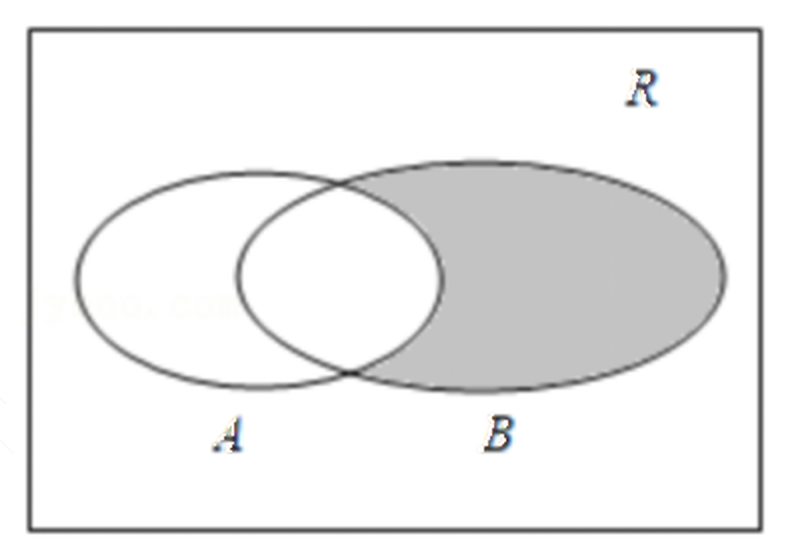
\includegraphics[width=0.36\textwidth]{figures/gao127_q4.png}
\end{center}

\ifanswer
\solbegin
\step{已知 $\R$ 是实数集，集合 $A=\{x\mid 1<x<2\}$, $B=\left\{x\mid 0<x<\frac32\right\}$,}
\step{阴影部分表示的集合是 $\overline A\cap B=\{x\mid 0<x\leqslant1\}$，即 $(0,1]$.}
\solend
\fi

\item 若集合 $\{x\mid (a-1)x^2+3x-2=0\}$ 有且仅有两个子集，则实数 $a$ 的值为\blankline[4.4em].

\ifanswer
\solbegin
\step{由题意得 $\{x\mid (a-1)x^2+3x-2=0\}$ 为单元素集，}
\step{所以 $a-1=0$ 或 $\begin{cases}a-1\neq0\\\triangle=9+8(a-1)=0\end{cases}$，所以 $a=1$ 或 $a=-\frac18$.}
\solend
\fi

\item 已知条件 $\alpha:x\leqslant m$，条件 $\beta:x^2-x\leqslant0$，若 $\alpha$ 是 $\beta$ 的必要条件，则实数 $m$ 的取值范围是为\blankline[4.4em].

\ifanswer
\solbegin
\step{不等式 $x^2-x\leqslant0$ 的解集为 $[0,1]$，}
\step{因为条件 $\alpha:x\leqslant m$，条件 $\beta:x^2-x\leqslant0$，且 $\alpha$ 是 $\beta$ 的必要条件，}
\step{所以集合 $[0,1]$ 是集合 $(-\infty,m]$ 的子集，得 $m\geqslant1$，实数 $m$ 的取值范围是 $[1,+\infty)$.}
\solend
\fi

\item 已知 $\alpha\in\{-2,-1,-\frac12,0,1,2\}$，若幂函数 $y=x^\alpha$ 在 $(0,+\infty)$ 是严格减函数且图像关于 $y$ 轴对称，则 $\alpha=$\blankline[4.4em].

\ifanswer
\solbegin
\step{幂函数 $y=x^\alpha$ 在 $(0,+\infty)$ 是严格减函数，则 $\alpha<0$，且图像关于 $y$ 轴对称，}
\step{则函数为偶函数，故 $\alpha=-2$.}
\solend
\fi

\item 若关于 $x$ 的不等式 $ax^2-3x+2<0$ 的解集不是空集，则实数 $a$ 的取值范围是\blankline[4.4em].

\ifanswer
\solbegin
\step{若 $a>0$，关于 $x$ 的不等式 $ax^2-3x+2<0$ 的解集不空，}
\step{所以一元二次方程 $ax^2-3x+2=0$ 的判别式大于零，}
\step{即 $(-3)^2-8a>0\Rightarrow a<\frac98$，结合 $a>0$ 得 $0<a<\frac98$；}
\step{若 $a\leqslant0$，则关于 $x$ 的不等式 $ax^2-3x+2<0$ 的解集不是空集；}
\step{综上，实数 $a$ 的取值范围是 $\left(-\infty,\frac98\right)$.}
\solend
\fi

\item 设 $\log_{18}2=a$，则 $\log_2 3$ 可用 $a$ 表示为\blankline[4.4em].

\ifanswer
\solbegin
\step{因为 $\log_{18}2=\frac{\log_2 2}{\log_2 18}=\frac1{1+2\log_2 3}=a$，则 $\log_2 3=\frac{1-a}{2a}$.}
\solend
\fi

\item 若关于 $x$ 的不等式 $ax^2+bx+c>0$ 解集为 $\left(-\frac12,3\right)$，则关于 $x$ 的不等式 $cx^2+bx+a<0$ 的解集为\blankline[4.4em].

\ifanswer
\solbegin
\step{由已知得 $a<0$，且 $ax^2+bx+c=a\left(x+\frac12\right)(x-3)$，}
\step{所以 $b=-\frac52 a, c=-\frac32 a$，}
\step{$cx^2+bx+a=-\frac a2(3x-1)(x+2)<0\Leftrightarrow(3x-1)(x+2)<0\Leftrightarrow -2<x<\frac13$，}
\step{故解集为 $\left(-2,\frac13\right)$.}
\solend
\fi

\item 设 $x\in\R$，则方程 $\lvert 2x+3\rvert-\lvert x-2\rvert=\lvert 3x+1\rvert$ 的解集为\blankline[4.4em].

\ifanswer
\solbegin
\step{当 $x\leqslant-\frac32$ 时，原式 $\Leftrightarrow -2x-3+x-2=-3x-1\Leftrightarrow x=2$，不合题意；}
\step{当 $-\frac32<x\leqslant-\frac13$ 时，原式 $\Leftrightarrow 2x+3+x-2=-3x-1\Leftrightarrow x=-\frac13$；}
\step{当 $-\frac13<x\leqslant2$ 时，原式 $\Leftrightarrow 2x+3+x-2=3x+1\Leftrightarrow 1=1$ 即恒成立；}
\step{当 $x>2$ 时，原式 $\Leftrightarrow 2x+3+2-x=3x+1\Leftrightarrow x=2$，不合题意；}
\step{故 $x\in\left[-\frac13,2\right]$.}
\solend
\fi

\item 若关于 $x$ 的不等式 $x^2-4mx+m<0$ 的解集为 $(x_1,x_2)$，若 $x_1>0,x_2>0$，试探究 $x_1+x_2,x_1x_2,x_1^2+x_2^2,\frac1{x_1}+\frac1{x_2}$ 的值，则 $4x_1+x_2$ 的最小值为\blankline[4.4em].

\ifanswer
\solbegin
\step{由题意得方程 $x^2-4mx+m=0$ 有两个相异的正实根 $x_1,x_2$，}
\step{故有 $\begin{cases}\triangle=16m^2-4m>0\\x_1+x_2=4m>0\\x_1\cdot x_2=m>0\end{cases}$，解得 $m>\frac14$，}
\step{则 $x_1^2+x_2^2=(x_1+x_2)^2-2x_1\cdot x_2=16m^2-2m$，$\frac1{x_1}+\frac1{x_2}=\frac{x_1+x_2}{x_1\cdot x_2}=4$，}
\step{则 $4x_1+x_2=\frac14(4x_1+x_2)\left(\frac1{x_1}+\frac1{x_2}\right)=\frac14\left(5+\frac{4x_1}{x_2}+\frac{x_2}{x_1}\right)\geqslant\frac94$，}
\step{当且仅当 $\frac{4x_1}{x_2}=\frac{x_2}{x_1}$ 时，即 $x_2=2x_1$ 时取等号，}
\step{由 $\begin{cases}x_2=2x_1\\\frac1{x_1}+\frac1{x_2}=4\end{cases}$，解得 $\begin{cases}x_1=\frac38\\x_2=\frac34\end{cases}$，于是 $m=x_1\cdot x_2=\frac9{32}\in\left(\frac14,+\infty\right)$，}
\step{即当 $m=\frac9{32}$ 时，$4x_1+x_2$ 取得最小值为 $\frac94$.}
\solend
\fi

\end{enumerate}

\bigsec{二、选择题}

\begin{enumerate}
\setcounter{enumi}{12}

\item 若 $a>0$, $a\neq1$, $M>0$, $N>0$，下列运算正确的是\mbox{（\quad）}

\keepwithprev
A. $\log_a\sqrt[N]{M}=\frac1N\log_a M$\qquad\qquad B. $(\log_a M)^N=N\log_a M$

C. $(\log_a M)\div(\log_a N)=\log_a(M-N)$\qquad\quad D. $\log_a M+\log_a N=\log_a(M+N)$

\ifanswer
\solbegin
\step{对于 $A$，$\log_a\sqrt[N]{M}=\log_a M^{\frac1N}=\frac1N\log_a M$，故 $A$ 正确；}
\step{对于 $B$，$(\log_a M)^N\neq N\log_a M=log_a M^n$，故 $B$ 错误；}
\step{对于 $C$，$(\log_a M)\div(\log_a N)\neq\log_a(M-N)$，故 $C$ 错误；}
\step{对于 $D$，$\log_a M+\log_a N=\log_a MN\neq\log_a(M+N)$，故 $D$ 错误.}
\step{故选 $A$.}
\solend
\fi

\item 下列不等式中正确的是\mbox{（\quad）}

\keepwithprev
A. 若 $a>b$，则 $ac^2>bc^2$\qquad\qquad B. 若 $a<b<0$，则 $a^2<b^2$

C. 若 $1<a<2$ 且 $0<b<3$，则 $1<a+b<5$\qquad D. 若 $\frac1a<1$，则 $a>1$

\ifanswer
\solbegin
\step{$C$ 中 $1+0<a+b<2+3$，即 $1<a+b<5$，正确.}
\step{$A$ 取 $c=0$ 时不成立；$B$ 应为 $a^2>b^2$；$D$ 取 $a=-1$ 时不成立. 故选 $C$.}
\solend
\fi

\item 已知 $y_1=x^3,y_2=x^2$，则下列说法正确的是\mbox{（\quad）}

\keepwithprev
A. $x\in(0,+\infty)$ 时，恒有 $y_1\geqslant y_2$

B. $y_1=x^3$ 与 $y_2=x^2$ 的函数图象仅有唯一交点

C. $x\in(0,1)$ 时，$y_1=x^3$ 图象在 $y_2=x^2$ 图象下方

D. 存在 $x_0\in(1,+\infty)$ 使得 $y_1=y_2$

\ifanswer
\solbegin
\step{$y_1-y_2=x^2(x-1)$，当 $0<x<1$ 时，$y_1<y_2$，故 $C$ 正确，$A$ 错误.}
\step{$y_1=y_2\Leftrightarrow x^2(x-1)=0\Leftrightarrow x=0$ 或 $x=1$，两图象有两个交点，故 $BD$ 错误.}
\step{故选 $C$.}
\solend
\fi

\item 已知非空集合 $A$、$B$ 满足两个条件：(1) $A\cup B=\{1,2,3,4,5,6,7\}$, $A\cap B=\varnothing$；(2) 若 $x\in A$，则 $x+1\in B$，则有序集合对 $(A,B)$ 的个数为\mbox{（\quad）}

\keepwithprev
A. $17$\qquad\qquad B. $18$\qquad\qquad C. $19$\qquad\qquad D. $20$

\ifanswer
\solbegin
\step{当 $A$ 为单元素集合时，有 6 种情况：}
\step{当 $A$ 为双元素集合时，$A=\{1,3\}, A=\{1,4\}, A=\{1,5\}, A=\{1,6\}, A=\{2,4\}$,}
\step{$A=\{2,5\}, A=\{2,6\}, A=\{3,5\}, A=\{3,6\}, A=\{4,6\}$，共 10 种情况；}
\step{当 $A$ 为三元素集合时，$A=\{1,3,5\}, A=\{1,3,6\}, A=\{1,4,6\}, A=\{2,4,6\}$，}
\step{共 4 种情况；}
\step{当 $A$ 为四元素集合时，不成立；}
\step{故有序集合对 $(A,B)$ 的个数为 20，故选 $D$.}
\solend
\fi

\end{enumerate}

\bigsec{三、解答题}

\begin{enumerate}
\setcounter{enumi}{16}

\item 已知 $x,y\in\R$，比较 $x^2+y^2$ 与 $2(2x-y)-5$ 的大小.

\ifanswer
\solbegin
\step{因为 $x^2+y^2-2(2x-y)+5=(x-2)^2+(y+1)^2\geqslant0$，}
\step{所以 $x^2+y^2\geqslant2(2x-y)-5$.}
\solend
\fi

\item 已知集合 $A=\{x\mid x^2+4x=0\}$，$B=\{x\mid x^2+2(a+1)x+a^2-1=0\}$.

(1) 若 $A$ 是 $B$ 的子集，求实数 $a$ 的值；

(2) 若 $B$ 是 $A$ 的子集，求实数 $a$ 的取值范围.

\ifanswer
\solbegin
\step{(1) 因为 $A=\{-4,0\}$，$B=\{x\mid x^2+2(a+1)x+a^2-1=0\}$，又 $A\subseteq B$，}
\step{所以 $A=B$，所以 $\begin{cases}-4+0=-2(a+1)\\-4\times0=a^2-1\end{cases}$，所以 $a=1$；}
\step{(2) 因为 $B$ 是 $A$ 的子集，所以 $B=\varnothing$ 或 $B=\{-4\}$ 或 $B=\{0\}$ 或 $B=\{-4,0\}$，}
\step{① $B=\varnothing$ 时，$\triangle=4(a+1)^2-4(a^2-1)<0$，所以 $a<-1$；}
\step{② $B=\{-4\}$ 时，$\begin{cases}-4+(-4)=-2(a+1)\\-4\times(-4)=a^2-1\end{cases}$，无解；}
\step{③ $B=\{0\}$ 时，$\begin{cases}0+0=-2(a+1)\\0\times0=a^2-1\end{cases}$，所以 $a=-1$；}
\step{④ $B=\{-4,0\}$ 时，由 (1) 得 $a=1$，}
\step{综上，实数 $a$ 的取值范围为 $(-\infty,-1]\cup\{1\}$.}
\solend
\fi

\item 某企业在现有设备下每日生产原先成本 $y$（单位：万元）与日产量 $x$（单位：吨）之间的函数关系式：$y=2x^2+(15-4k)x+120k+8$，近年来各部门都非常重视大气污染防治工作，为了配合环境卫生综合整治，该企业引进了除尘设备，每吨产品的除尘费用为 $k$ 万元，引进除尘设备后，当日产量 $x=1$ 时，总成本（总成本为原先成本和除尘费用之和）为 142 万元.

(1) 求 $k$ 的值；

(2) 求引进除尘设备后日产量为多少时，每吨产品的成本最小，并求出最小值.

\ifanswer
\solbegin
\step{(1) 该企业引进了除尘设备，}
\step{每日生产总成本 $h$（单位：万元）与日产量 $x$（单位：吨）之间的关系为}
\step{$h=2x^2+(15-4k)x+120k+8+kx=2x^2+(15-3k)x+120k+8$，}
\step{当日产量 $x=1$ 时，总成本为 $h=142$ 万元，}
\step{代入得 $2+(15-3k)+120k+8=142\Rightarrow k=1$，}
\step{(2) 由 (1) 得 $h=2x^2+12x+128$，}
\step{所以每吨产品的成本为 $w=\frac{2x^2+12x+128}{x}=2x+\frac{128}{x}+12$}
\step{$\geqslant2\sqrt{2x\cdot\frac{128}{x}}+12=44$，当且仅当 $2x=\frac{128}{x}$，即 $x=8$ 时，取等号，}
\step{所以引进除尘设备后日产量为 8 吨时，每吨产品的成本最小，}
\step{且最小值为 44 万元.}
\solend
\fi

\item 已知集合 $A=\{x\mid \lvert x-a\rvert<2\}$，集合 $B=\left\{x\mid\frac{2x-1}{x+2}<1\right\}$.

(1) 若 $a=2$，求 $A\cup B$；

(2) 若 $A\cap B=A$，求实数 $a$ 的取值范围.

\ifanswer
\solbegin
\step{(1) 若 $a=2$，则 $A=\{x\mid \lvert x-a\rvert<2\}=\{x\mid \lvert x-2\rvert<2\}=\{x\mid 0<x<4\}$，}
\step{由 $\frac{2x-1}{x+2}<1$ 得 $\frac{x-3}{x+2}<0$，即 $(x-3)(x+2)<0$，解得 $-2<x<3$，}
\step{所以 $B=\{x\mid -2<x<3\}$，所以 $A\cup B=\{x\mid -2<x<4\}$；}
\step{(2) 由 (1) 得 $B=\{x\mid -2<x<3\}$，}
\step{$A=\{x\mid \lvert x-a\rvert<2\}=\{x\mid a-2<x<a+2\}$，}
\step{若 $A\cap B=A$，则 $A\subseteq B$，则 $\begin{cases}a-2\geqslant-2\\a+2\leqslant3\end{cases}$，解得 $0\leqslant a\leqslant1$，}
\step{即实数 $a$ 的取值范围为 $[0,1]$.}
\solend
\fi

\item 已知自变量为 $x$ 的函数 $y=\frac{ax+b}{x+a}$，

(1) 若 $a=1$ 且 $b=2$，则函数 $y=\frac{ax+b}{x+a}$ 图像可由幂函数\blankline[4.4em]（写解析式）先沿 $x$ 轴方向\blankline[4.4em]平移\blankline[4.4em]个单位，再沿 $y$ 轴方向向上平移\blankline[4.4em]个单位得到；

(2) 当 $a>0$ 且 $b=-2$ 时不等式 $\frac{ax+b}{x+a}\leqslant\frac{2x^2}{x+a}$ 对 $x>0$ 恒成立，求实数 $a$ 的最大值；

(3) 若 $b=-2$ 且关于 $x$ 的不等式 $x^2\log_2\frac{4(a+1)}a+2x\log_2\frac{2a}{a+1}+\log_2\frac{(a+1)^2}{4a^2}\leqslant0$ 解集是单元素集，求出 $a$ 值，并求出函数 $y=\frac{ax-2}{x+a}$ 的对称中心.

\ifanswer
\solbegin
\step{(1) 已知自变量为 $x$ 的函数 $y=\frac{ax+b}{x+a}$，}
\step{当 $a=1$ 且 $b=2$ 时，$y=\frac{x+2}{x+1}=\frac{x+1+1}{x+1}=1+\frac1{x+1}$，}
\step{由幂函数 $y=\frac1x$，先沿 $x$ 轴方向向左平移一个单位，}
\step{再沿 $y$ 轴方向向上平移一个单位得到；}
\step{(2) 当 $a>0$ 且 $b=-2$ 时不等式 $\frac{ax+b}{x+a}\leqslant\frac{2x^2}{x+a}$ 即 $\frac{ax-2}{x+a}\leqslant\frac{2x^2}{x+a}$ 对 $x>0$ 恒成立，}
\step{因为 $a>0$ 且 $x>0$，所以 $x+a>0$，所以等价于 $ax-2\leqslant2x^2$ 对 $x>0$ 恒成立，}
\step{即 $2x^2-ax+2\geqslant0$ 对 $x>0$ 恒成立，}
\step{因为函数 $g(x)=2x^2-ax+2$ 的对称轴 $x=\frac a4>0$，且 $g(0)=2>0$，}
\step{则 $\begin{cases}\triangle=(-a)^2-4\times2\times2\leqslant0\\a>0\end{cases}$，解得 $0<a\leqslant4$，所以 $a$ 的最大值为 4；}
\step{(3) 关于 $x$ 的不等式 $x^2\log_2\frac{4(a+1)}a+2x\log_2\frac{2a}{a+1}+\log_2\frac{(a+1)^2}{4a^2}\leqslant0$ 解集}
\step{是单元素集，由 $\frac{4(a+1)}a>0$，则 $a>0$ 或 $a<-1$，}
\step{若 $\log_2\frac{4(a+1)}a=0$，则 $\frac{4(a+1)}a=1$，解得 $a=-\frac43$，}
\step{此时不等式为 $6x-6\leqslant0$，解得 $x\leqslant1$，不符合题意，}
\step{若 $\log_2\frac{4(a+1)}a>0$，即 $\frac{4(a+1)}a>1$，解得 $a>0$ 或 $a<-\frac43$，}
\step{则 $\triangle=\left(2\log_2\frac{2a}{a+1}\right)^2-4\log_2\frac{4(a+1)}a\cdot\log_2\frac{(a+1)^2}{4a^2}=0$，}
\step{令 $\log_2\frac{2a}{a+1}=t$，则 $t^2-(3-t)(-2t)=0$，解得 $t=0$ 或 $t=6$，}
\step{当 $\log_2\frac{2a}{a+1}=0$，解得 $a=1$，$\log_2\frac{2a}{a+1}=6$，解得 $a=-\frac{32}{31}$(舍去)，所以 $a=1$，}
\step{则函数 $y=\frac{ax-2}{x+a}$ 即为 $y=\frac{x-2}{x+1}=\frac{x+1-3}{x+1}=1+\frac{-3}{x+1}$，}
\step{对称中心为 $(-1,1)$.}
\solend
\fi

\end{enumerate}

\end{document}
"
% 紧凑版：xelatex "\def\iscompact{1}% 高一127_南汇一中_期中.tex
%   —— 高一上数学“2026-2027 年南汇一中高一上期中”（试卷版/答案版）
% 试卷版：xelatex 高一127_南汇一中_期中.tex
% 答案版：xelatex "\def\isanswer{1}% 高一127_南汇一中_期中.tex
%   —— 高一上数学“2026-2027 年南汇一中高一上期中”（试卷版/答案版）
% 试卷版：xelatex 高一127_南汇一中_期中.tex
% 答案版：xelatex "\def\isanswer{1}\input{高一127_南汇一中_期中.tex}"
% 紧凑版：xelatex "\def\iscompact{1}\input{高一127_南汇一中_期中.tex}"
%
% 原始材料：微信公众号“魔都数学加油站”文章，作者破晓，2026-11-11 18:35 发布；
% 连载“27学年高一127”，原文标题“27学年高一127——2026-2027年上海市南汇一中高一上期中”；
% 原文链接：https://mp.weixin.qq.com/s/nozIwRgeWSKPCPSiqfCm2Q。
% 正文为 9 张 PNG 页（01、02、03、09 为 2560×3620，04、05、06、07、08 为 4762×6735），
% 题目下印有【解析】，为讲评版。题目、解析均据原图转录；
% 卷面粉红色水印“魔都数学加油站”及公众号页脚未录入。全卷仅第 4 题一幅插图。
% 第 09 页只有一行“对称中心为(-1,1).”及水印，是第 08 页末行的续尾页。
%
% 卷首标题：原卷印作“2026-2027 年南汇一中高一上期中”（公众号标题中的“上海市”
% 卷面标题行没有，本稿照卷面），年份区间按全稿惯例排 en dash；原卷未印副标题，
% 本卷为期中卷、跨三章，按题目内容标为“集合与常用逻辑用语、不等式、函数”
% （第 4/5/6/16/18/20 题为集合与常用逻辑用语，第 8/10/11/12/14/17 题为不等式，
% 第 3/7/9/13/15/19/21 题为函数；与 106、125 同为期中复习卷，口径相同）。
%
% 与原卷的排版差异：
%   ① 原文从第 3 题起，填空题编号为 3—12、选择题为 13—16、解答题为 17—21，本稿保留原题号；
%   ② 原卷每题下直接印【解析】，本稿按全稿惯例置于答案版；四道选择题答案均在解析末句
%      “故选 …”，括号内留空、不另提 \ans{}；全卷无只印【答案】或括号内答案的题；
%   ③ 原卷未印副标题，本稿按“知识模块”口径补出；
%   ④ 原卷填空横线按全稿惯例排为 \blankline[4.4em]；选择题括号排 \mbox{（\quad）}、
%      选项段前按惯例加 \keepwithprev；解答题不留作答区（原卷为讲评版，与 109—125 同）；
%      第 21 题 (1) 的四处填空横线亦排 \blankline[4.4em]；
%   ⑤ 原卷数集排斜体 $R$，按全稿惯例改 \R；绝对值排 \lvert…\rvert，集合描述竖线排 \mid；
%      补集记号照原卷上划线排 \overline{A}；不等号一律 \leqslant / \geqslant；
%   ⑥ 第 4 题插图原在题干右侧，本稿按全稿惯例移至题干之后居中排（取原卷截图、
%      去粉色水印后 2× LANCZOS 放大，存 figures/gao127_q4.png），三版都出；
%      并在该题 \item 前加 \needvspace{} 守卫，把题干与插图整块推走；
%   ⑦ 原卷子题编号 (1)(2)(3) 与括号按全稿惯例排；“（单位：万元）”“（写解析式）”
%      用全角括号，第 21 题 (3) 解析“(舍去)”用半角括号，均照录；
%   ⑧ 第 09 页仅一行“对称中心为(-1,1).”为第 08 页末行之续尾，本稿按原卷印刷行
%      另起一条 \step，置于答案版最后一题解析之末。
%
% 子集符号：第 18 题 (1) 解析 $A\subseteq B$、第 20 题 (2) 解析 $A\subseteq B$ 均印有
%   下划线，照录 \subseteq；全卷无 \subset。回原图放大逐处确认。
%
% 判别式字形：本卷 5 处判别式（第 5 题解析 cases 内 $\triangle=9+8(a-1)=0$、
%   第 12 题解析 cases 内 $\triangle=16m^2-4m>0$、第 18 题① $\triangle=4(a+1)^2-4(a^2-1)<0$、
%   第 21 题 (2) cases 内 $\triangle=(-a)^2-4\times2\times2\leqslant0$、
%   第 21 题 (3) $\triangle=\left(2\log_2\frac{2a}{a+1}\right)^2-\cdots=0$）均排等边扁三角，
%   照录 \triangle；逐处回原图全分辨率放大确认，无高三角 $\Delta$（与 高一26 排 $\Delta$ 不同）。
%
% 原卷存疑照录：
%   第 6 题题干作“则实数 $m$ 的取值范围是为____”（“是为”叠用，疑衍一字），照录；
%   第 12 题题干“试探究 $x_1+x_2, x_1x_2, x_1^2+x_2^2, \frac1{x_1}+\frac1{x_2}$ 的值，
%     则 $4x_1+x_2$ 的最小值为____”与后文衔接突兀，照录；
%   第 13 题解析 B 作“$(\log_a M)^N\neq N\log_a M=log_a M^n$”，后一 log 为斜体、
%     指数作小写 $n$，与前式 $N\log_a M$ 及题干 $N$ 不一致，照录；
%   第 13 题解析 A、B、C 三步句末用“；”，D 步句末用“.”，标点不一致，照录；
%   第 15 题解析“故 $BD$ 错误.”两选项字母连写、无顿号，照录；
%   第 7 题题干及解析用“图像”，第 15 题 B、C 及解析用“图象”，全卷两种写法混用，照录未统一；
%   第 21 题 (3) 题干“求出 $a$ 值”（通常作“求出 $a$ 的值”），照录；
%   第 21 题 (3) 解析“解得 $a=1$，$\log_2\frac{2a}{a+1}=6$，解得 $a=-\frac{32}{31}$(舍去)，
%     所以 $a=1$”两个“解得”并列、且舍去值用半角括号，照录；
%   第 09 页“对称中心为(-1,1).”用半角括号与半角句点，照录；
%   第 8 题解析“若 $a\leqslant0$，则关于 $x$ 的不等式 $ax^2-3x+2<0$ 的解集不是空集；”
%     未给理由直接断言，照录；
%   第 18 题 (1) 由 $A\subseteq B$ 直接得 $A=B$，照录。
%
% 行数核对：逐题数 \step 条数，合计 95 条（Q3：1；Q4：2；Q5：2；Q6：3；Q7：2；
% Q8：5；Q9：1；Q10：4；Q11：5；Q12：7；Q13：5；Q14：2；Q15：3；Q16：7；
% Q17：2；Q18：8；Q19：10；Q20：7；Q21：19），与原卷印刷行逐题相等
% （cases 块作一个印刷行计；Q21 第 19 行为第 09 页续尾）。全卷 19 题均印【解析】，
% 无只印【答案】或括号内答案的题，故 \ans{} 为 0；四道选择题括号内留空、不另提 \ans{}。
%
\documentclass[a4paper,11pt]{article}
\usepackage{common}

\begin{document}

\examtitlest[3]{2026--2027 年南汇一中高一上期中}{集合与常用逻辑用语、不等式、函数}

\bigsec{一、填空题}

\begin{enumerate}
\setcounter{enumi}{2}

\item 把 $\sqrt[4]{a\sqrt a}(a>0)$ 化成有理数指数幂的形式为\blankline[4.4em].

\ifanswer
\solbegin
\step{$\sqrt[4]{a\sqrt a}=(a\cdot a^{\frac12})^{\frac14}=a^{\frac38}$.}
\solend
\fi

\needvspace{6.5cm}
\item 已知集合 $A=\{x\mid 1<x<2\}$, $B=\left\{x\mid 0<x<\frac32\right\}$, 则如图阴影部分表示的集合是\blankline[4.4em].

\begin{center}
% 图取原卷截图（第 1 页题干右侧）、去水印后 2× LANCZOS 放大，本稿移至题干之后
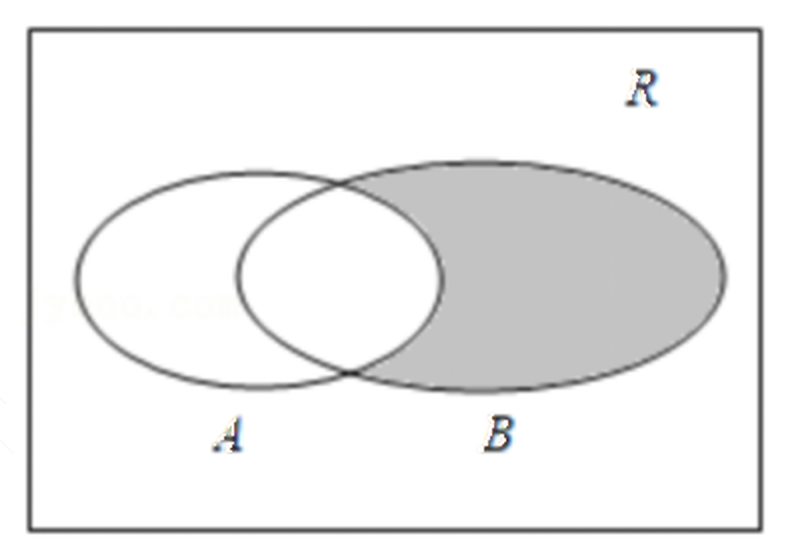
\includegraphics[width=0.36\textwidth]{figures/gao127_q4.png}
\end{center}

\ifanswer
\solbegin
\step{已知 $\R$ 是实数集，集合 $A=\{x\mid 1<x<2\}$, $B=\left\{x\mid 0<x<\frac32\right\}$,}
\step{阴影部分表示的集合是 $\overline A\cap B=\{x\mid 0<x\leqslant1\}$，即 $(0,1]$.}
\solend
\fi

\item 若集合 $\{x\mid (a-1)x^2+3x-2=0\}$ 有且仅有两个子集，则实数 $a$ 的值为\blankline[4.4em].

\ifanswer
\solbegin
\step{由题意得 $\{x\mid (a-1)x^2+3x-2=0\}$ 为单元素集，}
\step{所以 $a-1=0$ 或 $\begin{cases}a-1\neq0\\\triangle=9+8(a-1)=0\end{cases}$，所以 $a=1$ 或 $a=-\frac18$.}
\solend
\fi

\item 已知条件 $\alpha:x\leqslant m$，条件 $\beta:x^2-x\leqslant0$，若 $\alpha$ 是 $\beta$ 的必要条件，则实数 $m$ 的取值范围是为\blankline[4.4em].

\ifanswer
\solbegin
\step{不等式 $x^2-x\leqslant0$ 的解集为 $[0,1]$，}
\step{因为条件 $\alpha:x\leqslant m$，条件 $\beta:x^2-x\leqslant0$，且 $\alpha$ 是 $\beta$ 的必要条件，}
\step{所以集合 $[0,1]$ 是集合 $(-\infty,m]$ 的子集，得 $m\geqslant1$，实数 $m$ 的取值范围是 $[1,+\infty)$.}
\solend
\fi

\item 已知 $\alpha\in\{-2,-1,-\frac12,0,1,2\}$，若幂函数 $y=x^\alpha$ 在 $(0,+\infty)$ 是严格减函数且图像关于 $y$ 轴对称，则 $\alpha=$\blankline[4.4em].

\ifanswer
\solbegin
\step{幂函数 $y=x^\alpha$ 在 $(0,+\infty)$ 是严格减函数，则 $\alpha<0$，且图像关于 $y$ 轴对称，}
\step{则函数为偶函数，故 $\alpha=-2$.}
\solend
\fi

\item 若关于 $x$ 的不等式 $ax^2-3x+2<0$ 的解集不是空集，则实数 $a$ 的取值范围是\blankline[4.4em].

\ifanswer
\solbegin
\step{若 $a>0$，关于 $x$ 的不等式 $ax^2-3x+2<0$ 的解集不空，}
\step{所以一元二次方程 $ax^2-3x+2=0$ 的判别式大于零，}
\step{即 $(-3)^2-8a>0\Rightarrow a<\frac98$，结合 $a>0$ 得 $0<a<\frac98$；}
\step{若 $a\leqslant0$，则关于 $x$ 的不等式 $ax^2-3x+2<0$ 的解集不是空集；}
\step{综上，实数 $a$ 的取值范围是 $\left(-\infty,\frac98\right)$.}
\solend
\fi

\item 设 $\log_{18}2=a$，则 $\log_2 3$ 可用 $a$ 表示为\blankline[4.4em].

\ifanswer
\solbegin
\step{因为 $\log_{18}2=\frac{\log_2 2}{\log_2 18}=\frac1{1+2\log_2 3}=a$，则 $\log_2 3=\frac{1-a}{2a}$.}
\solend
\fi

\item 若关于 $x$ 的不等式 $ax^2+bx+c>0$ 解集为 $\left(-\frac12,3\right)$，则关于 $x$ 的不等式 $cx^2+bx+a<0$ 的解集为\blankline[4.4em].

\ifanswer
\solbegin
\step{由已知得 $a<0$，且 $ax^2+bx+c=a\left(x+\frac12\right)(x-3)$，}
\step{所以 $b=-\frac52 a, c=-\frac32 a$，}
\step{$cx^2+bx+a=-\frac a2(3x-1)(x+2)<0\Leftrightarrow(3x-1)(x+2)<0\Leftrightarrow -2<x<\frac13$，}
\step{故解集为 $\left(-2,\frac13\right)$.}
\solend
\fi

\item 设 $x\in\R$，则方程 $\lvert 2x+3\rvert-\lvert x-2\rvert=\lvert 3x+1\rvert$ 的解集为\blankline[4.4em].

\ifanswer
\solbegin
\step{当 $x\leqslant-\frac32$ 时，原式 $\Leftrightarrow -2x-3+x-2=-3x-1\Leftrightarrow x=2$，不合题意；}
\step{当 $-\frac32<x\leqslant-\frac13$ 时，原式 $\Leftrightarrow 2x+3+x-2=-3x-1\Leftrightarrow x=-\frac13$；}
\step{当 $-\frac13<x\leqslant2$ 时，原式 $\Leftrightarrow 2x+3+x-2=3x+1\Leftrightarrow 1=1$ 即恒成立；}
\step{当 $x>2$ 时，原式 $\Leftrightarrow 2x+3+2-x=3x+1\Leftrightarrow x=2$，不合题意；}
\step{故 $x\in\left[-\frac13,2\right]$.}
\solend
\fi

\item 若关于 $x$ 的不等式 $x^2-4mx+m<0$ 的解集为 $(x_1,x_2)$，若 $x_1>0,x_2>0$，试探究 $x_1+x_2,x_1x_2,x_1^2+x_2^2,\frac1{x_1}+\frac1{x_2}$ 的值，则 $4x_1+x_2$ 的最小值为\blankline[4.4em].

\ifanswer
\solbegin
\step{由题意得方程 $x^2-4mx+m=0$ 有两个相异的正实根 $x_1,x_2$，}
\step{故有 $\begin{cases}\triangle=16m^2-4m>0\\x_1+x_2=4m>0\\x_1\cdot x_2=m>0\end{cases}$，解得 $m>\frac14$，}
\step{则 $x_1^2+x_2^2=(x_1+x_2)^2-2x_1\cdot x_2=16m^2-2m$，$\frac1{x_1}+\frac1{x_2}=\frac{x_1+x_2}{x_1\cdot x_2}=4$，}
\step{则 $4x_1+x_2=\frac14(4x_1+x_2)\left(\frac1{x_1}+\frac1{x_2}\right)=\frac14\left(5+\frac{4x_1}{x_2}+\frac{x_2}{x_1}\right)\geqslant\frac94$，}
\step{当且仅当 $\frac{4x_1}{x_2}=\frac{x_2}{x_1}$ 时，即 $x_2=2x_1$ 时取等号，}
\step{由 $\begin{cases}x_2=2x_1\\\frac1{x_1}+\frac1{x_2}=4\end{cases}$，解得 $\begin{cases}x_1=\frac38\\x_2=\frac34\end{cases}$，于是 $m=x_1\cdot x_2=\frac9{32}\in\left(\frac14,+\infty\right)$，}
\step{即当 $m=\frac9{32}$ 时，$4x_1+x_2$ 取得最小值为 $\frac94$.}
\solend
\fi

\end{enumerate}

\bigsec{二、选择题}

\begin{enumerate}
\setcounter{enumi}{12}

\item 若 $a>0$, $a\neq1$, $M>0$, $N>0$，下列运算正确的是\mbox{（\quad）}

\keepwithprev
A. $\log_a\sqrt[N]{M}=\frac1N\log_a M$\qquad\qquad B. $(\log_a M)^N=N\log_a M$

C. $(\log_a M)\div(\log_a N)=\log_a(M-N)$\qquad\quad D. $\log_a M+\log_a N=\log_a(M+N)$

\ifanswer
\solbegin
\step{对于 $A$，$\log_a\sqrt[N]{M}=\log_a M^{\frac1N}=\frac1N\log_a M$，故 $A$ 正确；}
\step{对于 $B$，$(\log_a M)^N\neq N\log_a M=log_a M^n$，故 $B$ 错误；}
\step{对于 $C$，$(\log_a M)\div(\log_a N)\neq\log_a(M-N)$，故 $C$ 错误；}
\step{对于 $D$，$\log_a M+\log_a N=\log_a MN\neq\log_a(M+N)$，故 $D$ 错误.}
\step{故选 $A$.}
\solend
\fi

\item 下列不等式中正确的是\mbox{（\quad）}

\keepwithprev
A. 若 $a>b$，则 $ac^2>bc^2$\qquad\qquad B. 若 $a<b<0$，则 $a^2<b^2$

C. 若 $1<a<2$ 且 $0<b<3$，则 $1<a+b<5$\qquad D. 若 $\frac1a<1$，则 $a>1$

\ifanswer
\solbegin
\step{$C$ 中 $1+0<a+b<2+3$，即 $1<a+b<5$，正确.}
\step{$A$ 取 $c=0$ 时不成立；$B$ 应为 $a^2>b^2$；$D$ 取 $a=-1$ 时不成立. 故选 $C$.}
\solend
\fi

\item 已知 $y_1=x^3,y_2=x^2$，则下列说法正确的是\mbox{（\quad）}

\keepwithprev
A. $x\in(0,+\infty)$ 时，恒有 $y_1\geqslant y_2$

B. $y_1=x^3$ 与 $y_2=x^2$ 的函数图象仅有唯一交点

C. $x\in(0,1)$ 时，$y_1=x^3$ 图象在 $y_2=x^2$ 图象下方

D. 存在 $x_0\in(1,+\infty)$ 使得 $y_1=y_2$

\ifanswer
\solbegin
\step{$y_1-y_2=x^2(x-1)$，当 $0<x<1$ 时，$y_1<y_2$，故 $C$ 正确，$A$ 错误.}
\step{$y_1=y_2\Leftrightarrow x^2(x-1)=0\Leftrightarrow x=0$ 或 $x=1$，两图象有两个交点，故 $BD$ 错误.}
\step{故选 $C$.}
\solend
\fi

\item 已知非空集合 $A$、$B$ 满足两个条件：(1) $A\cup B=\{1,2,3,4,5,6,7\}$, $A\cap B=\varnothing$；(2) 若 $x\in A$，则 $x+1\in B$，则有序集合对 $(A,B)$ 的个数为\mbox{（\quad）}

\keepwithprev
A. $17$\qquad\qquad B. $18$\qquad\qquad C. $19$\qquad\qquad D. $20$

\ifanswer
\solbegin
\step{当 $A$ 为单元素集合时，有 6 种情况：}
\step{当 $A$ 为双元素集合时，$A=\{1,3\}, A=\{1,4\}, A=\{1,5\}, A=\{1,6\}, A=\{2,4\}$,}
\step{$A=\{2,5\}, A=\{2,6\}, A=\{3,5\}, A=\{3,6\}, A=\{4,6\}$，共 10 种情况；}
\step{当 $A$ 为三元素集合时，$A=\{1,3,5\}, A=\{1,3,6\}, A=\{1,4,6\}, A=\{2,4,6\}$，}
\step{共 4 种情况；}
\step{当 $A$ 为四元素集合时，不成立；}
\step{故有序集合对 $(A,B)$ 的个数为 20，故选 $D$.}
\solend
\fi

\end{enumerate}

\bigsec{三、解答题}

\begin{enumerate}
\setcounter{enumi}{16}

\item 已知 $x,y\in\R$，比较 $x^2+y^2$ 与 $2(2x-y)-5$ 的大小.

\ifanswer
\solbegin
\step{因为 $x^2+y^2-2(2x-y)+5=(x-2)^2+(y+1)^2\geqslant0$，}
\step{所以 $x^2+y^2\geqslant2(2x-y)-5$.}
\solend
\fi

\item 已知集合 $A=\{x\mid x^2+4x=0\}$，$B=\{x\mid x^2+2(a+1)x+a^2-1=0\}$.

(1) 若 $A$ 是 $B$ 的子集，求实数 $a$ 的值；

(2) 若 $B$ 是 $A$ 的子集，求实数 $a$ 的取值范围.

\ifanswer
\solbegin
\step{(1) 因为 $A=\{-4,0\}$，$B=\{x\mid x^2+2(a+1)x+a^2-1=0\}$，又 $A\subseteq B$，}
\step{所以 $A=B$，所以 $\begin{cases}-4+0=-2(a+1)\\-4\times0=a^2-1\end{cases}$，所以 $a=1$；}
\step{(2) 因为 $B$ 是 $A$ 的子集，所以 $B=\varnothing$ 或 $B=\{-4\}$ 或 $B=\{0\}$ 或 $B=\{-4,0\}$，}
\step{① $B=\varnothing$ 时，$\triangle=4(a+1)^2-4(a^2-1)<0$，所以 $a<-1$；}
\step{② $B=\{-4\}$ 时，$\begin{cases}-4+(-4)=-2(a+1)\\-4\times(-4)=a^2-1\end{cases}$，无解；}
\step{③ $B=\{0\}$ 时，$\begin{cases}0+0=-2(a+1)\\0\times0=a^2-1\end{cases}$，所以 $a=-1$；}
\step{④ $B=\{-4,0\}$ 时，由 (1) 得 $a=1$，}
\step{综上，实数 $a$ 的取值范围为 $(-\infty,-1]\cup\{1\}$.}
\solend
\fi

\item 某企业在现有设备下每日生产原先成本 $y$（单位：万元）与日产量 $x$（单位：吨）之间的函数关系式：$y=2x^2+(15-4k)x+120k+8$，近年来各部门都非常重视大气污染防治工作，为了配合环境卫生综合整治，该企业引进了除尘设备，每吨产品的除尘费用为 $k$ 万元，引进除尘设备后，当日产量 $x=1$ 时，总成本（总成本为原先成本和除尘费用之和）为 142 万元.

(1) 求 $k$ 的值；

(2) 求引进除尘设备后日产量为多少时，每吨产品的成本最小，并求出最小值.

\ifanswer
\solbegin
\step{(1) 该企业引进了除尘设备，}
\step{每日生产总成本 $h$（单位：万元）与日产量 $x$（单位：吨）之间的关系为}
\step{$h=2x^2+(15-4k)x+120k+8+kx=2x^2+(15-3k)x+120k+8$，}
\step{当日产量 $x=1$ 时，总成本为 $h=142$ 万元，}
\step{代入得 $2+(15-3k)+120k+8=142\Rightarrow k=1$，}
\step{(2) 由 (1) 得 $h=2x^2+12x+128$，}
\step{所以每吨产品的成本为 $w=\frac{2x^2+12x+128}{x}=2x+\frac{128}{x}+12$}
\step{$\geqslant2\sqrt{2x\cdot\frac{128}{x}}+12=44$，当且仅当 $2x=\frac{128}{x}$，即 $x=8$ 时，取等号，}
\step{所以引进除尘设备后日产量为 8 吨时，每吨产品的成本最小，}
\step{且最小值为 44 万元.}
\solend
\fi

\item 已知集合 $A=\{x\mid \lvert x-a\rvert<2\}$，集合 $B=\left\{x\mid\frac{2x-1}{x+2}<1\right\}$.

(1) 若 $a=2$，求 $A\cup B$；

(2) 若 $A\cap B=A$，求实数 $a$ 的取值范围.

\ifanswer
\solbegin
\step{(1) 若 $a=2$，则 $A=\{x\mid \lvert x-a\rvert<2\}=\{x\mid \lvert x-2\rvert<2\}=\{x\mid 0<x<4\}$，}
\step{由 $\frac{2x-1}{x+2}<1$ 得 $\frac{x-3}{x+2}<0$，即 $(x-3)(x+2)<0$，解得 $-2<x<3$，}
\step{所以 $B=\{x\mid -2<x<3\}$，所以 $A\cup B=\{x\mid -2<x<4\}$；}
\step{(2) 由 (1) 得 $B=\{x\mid -2<x<3\}$，}
\step{$A=\{x\mid \lvert x-a\rvert<2\}=\{x\mid a-2<x<a+2\}$，}
\step{若 $A\cap B=A$，则 $A\subseteq B$，则 $\begin{cases}a-2\geqslant-2\\a+2\leqslant3\end{cases}$，解得 $0\leqslant a\leqslant1$，}
\step{即实数 $a$ 的取值范围为 $[0,1]$.}
\solend
\fi

\item 已知自变量为 $x$ 的函数 $y=\frac{ax+b}{x+a}$，

(1) 若 $a=1$ 且 $b=2$，则函数 $y=\frac{ax+b}{x+a}$ 图像可由幂函数\blankline[4.4em]（写解析式）先沿 $x$ 轴方向\blankline[4.4em]平移\blankline[4.4em]个单位，再沿 $y$ 轴方向向上平移\blankline[4.4em]个单位得到；

(2) 当 $a>0$ 且 $b=-2$ 时不等式 $\frac{ax+b}{x+a}\leqslant\frac{2x^2}{x+a}$ 对 $x>0$ 恒成立，求实数 $a$ 的最大值；

(3) 若 $b=-2$ 且关于 $x$ 的不等式 $x^2\log_2\frac{4(a+1)}a+2x\log_2\frac{2a}{a+1}+\log_2\frac{(a+1)^2}{4a^2}\leqslant0$ 解集是单元素集，求出 $a$ 值，并求出函数 $y=\frac{ax-2}{x+a}$ 的对称中心.

\ifanswer
\solbegin
\step{(1) 已知自变量为 $x$ 的函数 $y=\frac{ax+b}{x+a}$，}
\step{当 $a=1$ 且 $b=2$ 时，$y=\frac{x+2}{x+1}=\frac{x+1+1}{x+1}=1+\frac1{x+1}$，}
\step{由幂函数 $y=\frac1x$，先沿 $x$ 轴方向向左平移一个单位，}
\step{再沿 $y$ 轴方向向上平移一个单位得到；}
\step{(2) 当 $a>0$ 且 $b=-2$ 时不等式 $\frac{ax+b}{x+a}\leqslant\frac{2x^2}{x+a}$ 即 $\frac{ax-2}{x+a}\leqslant\frac{2x^2}{x+a}$ 对 $x>0$ 恒成立，}
\step{因为 $a>0$ 且 $x>0$，所以 $x+a>0$，所以等价于 $ax-2\leqslant2x^2$ 对 $x>0$ 恒成立，}
\step{即 $2x^2-ax+2\geqslant0$ 对 $x>0$ 恒成立，}
\step{因为函数 $g(x)=2x^2-ax+2$ 的对称轴 $x=\frac a4>0$，且 $g(0)=2>0$，}
\step{则 $\begin{cases}\triangle=(-a)^2-4\times2\times2\leqslant0\\a>0\end{cases}$，解得 $0<a\leqslant4$，所以 $a$ 的最大值为 4；}
\step{(3) 关于 $x$ 的不等式 $x^2\log_2\frac{4(a+1)}a+2x\log_2\frac{2a}{a+1}+\log_2\frac{(a+1)^2}{4a^2}\leqslant0$ 解集}
\step{是单元素集，由 $\frac{4(a+1)}a>0$，则 $a>0$ 或 $a<-1$，}
\step{若 $\log_2\frac{4(a+1)}a=0$，则 $\frac{4(a+1)}a=1$，解得 $a=-\frac43$，}
\step{此时不等式为 $6x-6\leqslant0$，解得 $x\leqslant1$，不符合题意，}
\step{若 $\log_2\frac{4(a+1)}a>0$，即 $\frac{4(a+1)}a>1$，解得 $a>0$ 或 $a<-\frac43$，}
\step{则 $\triangle=\left(2\log_2\frac{2a}{a+1}\right)^2-4\log_2\frac{4(a+1)}a\cdot\log_2\frac{(a+1)^2}{4a^2}=0$，}
\step{令 $\log_2\frac{2a}{a+1}=t$，则 $t^2-(3-t)(-2t)=0$，解得 $t=0$ 或 $t=6$，}
\step{当 $\log_2\frac{2a}{a+1}=0$，解得 $a=1$，$\log_2\frac{2a}{a+1}=6$，解得 $a=-\frac{32}{31}$(舍去)，所以 $a=1$，}
\step{则函数 $y=\frac{ax-2}{x+a}$ 即为 $y=\frac{x-2}{x+1}=\frac{x+1-3}{x+1}=1+\frac{-3}{x+1}$，}
\step{对称中心为 $(-1,1)$.}
\solend
\fi

\end{enumerate}

\end{document}
"
% 紧凑版：xelatex "\def\iscompact{1}% 高一127_南汇一中_期中.tex
%   —— 高一上数学“2026-2027 年南汇一中高一上期中”（试卷版/答案版）
% 试卷版：xelatex 高一127_南汇一中_期中.tex
% 答案版：xelatex "\def\isanswer{1}\input{高一127_南汇一中_期中.tex}"
% 紧凑版：xelatex "\def\iscompact{1}\input{高一127_南汇一中_期中.tex}"
%
% 原始材料：微信公众号“魔都数学加油站”文章，作者破晓，2026-11-11 18:35 发布；
% 连载“27学年高一127”，原文标题“27学年高一127——2026-2027年上海市南汇一中高一上期中”；
% 原文链接：https://mp.weixin.qq.com/s/nozIwRgeWSKPCPSiqfCm2Q。
% 正文为 9 张 PNG 页（01、02、03、09 为 2560×3620，04、05、06、07、08 为 4762×6735），
% 题目下印有【解析】，为讲评版。题目、解析均据原图转录；
% 卷面粉红色水印“魔都数学加油站”及公众号页脚未录入。全卷仅第 4 题一幅插图。
% 第 09 页只有一行“对称中心为(-1,1).”及水印，是第 08 页末行的续尾页。
%
% 卷首标题：原卷印作“2026-2027 年南汇一中高一上期中”（公众号标题中的“上海市”
% 卷面标题行没有，本稿照卷面），年份区间按全稿惯例排 en dash；原卷未印副标题，
% 本卷为期中卷、跨三章，按题目内容标为“集合与常用逻辑用语、不等式、函数”
% （第 4/5/6/16/18/20 题为集合与常用逻辑用语，第 8/10/11/12/14/17 题为不等式，
% 第 3/7/9/13/15/19/21 题为函数；与 106、125 同为期中复习卷，口径相同）。
%
% 与原卷的排版差异：
%   ① 原文从第 3 题起，填空题编号为 3—12、选择题为 13—16、解答题为 17—21，本稿保留原题号；
%   ② 原卷每题下直接印【解析】，本稿按全稿惯例置于答案版；四道选择题答案均在解析末句
%      “故选 …”，括号内留空、不另提 \ans{}；全卷无只印【答案】或括号内答案的题；
%   ③ 原卷未印副标题，本稿按“知识模块”口径补出；
%   ④ 原卷填空横线按全稿惯例排为 \blankline[4.4em]；选择题括号排 \mbox{（\quad）}、
%      选项段前按惯例加 \keepwithprev；解答题不留作答区（原卷为讲评版，与 109—125 同）；
%      第 21 题 (1) 的四处填空横线亦排 \blankline[4.4em]；
%   ⑤ 原卷数集排斜体 $R$，按全稿惯例改 \R；绝对值排 \lvert…\rvert，集合描述竖线排 \mid；
%      补集记号照原卷上划线排 \overline{A}；不等号一律 \leqslant / \geqslant；
%   ⑥ 第 4 题插图原在题干右侧，本稿按全稿惯例移至题干之后居中排（取原卷截图、
%      去粉色水印后 2× LANCZOS 放大，存 figures/gao127_q4.png），三版都出；
%      并在该题 \item 前加 \needvspace{} 守卫，把题干与插图整块推走；
%   ⑦ 原卷子题编号 (1)(2)(3) 与括号按全稿惯例排；“（单位：万元）”“（写解析式）”
%      用全角括号，第 21 题 (3) 解析“(舍去)”用半角括号，均照录；
%   ⑧ 第 09 页仅一行“对称中心为(-1,1).”为第 08 页末行之续尾，本稿按原卷印刷行
%      另起一条 \step，置于答案版最后一题解析之末。
%
% 子集符号：第 18 题 (1) 解析 $A\subseteq B$、第 20 题 (2) 解析 $A\subseteq B$ 均印有
%   下划线，照录 \subseteq；全卷无 \subset。回原图放大逐处确认。
%
% 判别式字形：本卷 5 处判别式（第 5 题解析 cases 内 $\triangle=9+8(a-1)=0$、
%   第 12 题解析 cases 内 $\triangle=16m^2-4m>0$、第 18 题① $\triangle=4(a+1)^2-4(a^2-1)<0$、
%   第 21 题 (2) cases 内 $\triangle=(-a)^2-4\times2\times2\leqslant0$、
%   第 21 题 (3) $\triangle=\left(2\log_2\frac{2a}{a+1}\right)^2-\cdots=0$）均排等边扁三角，
%   照录 \triangle；逐处回原图全分辨率放大确认，无高三角 $\Delta$（与 高一26 排 $\Delta$ 不同）。
%
% 原卷存疑照录：
%   第 6 题题干作“则实数 $m$ 的取值范围是为____”（“是为”叠用，疑衍一字），照录；
%   第 12 题题干“试探究 $x_1+x_2, x_1x_2, x_1^2+x_2^2, \frac1{x_1}+\frac1{x_2}$ 的值，
%     则 $4x_1+x_2$ 的最小值为____”与后文衔接突兀，照录；
%   第 13 题解析 B 作“$(\log_a M)^N\neq N\log_a M=log_a M^n$”，后一 log 为斜体、
%     指数作小写 $n$，与前式 $N\log_a M$ 及题干 $N$ 不一致，照录；
%   第 13 题解析 A、B、C 三步句末用“；”，D 步句末用“.”，标点不一致，照录；
%   第 15 题解析“故 $BD$ 错误.”两选项字母连写、无顿号，照录；
%   第 7 题题干及解析用“图像”，第 15 题 B、C 及解析用“图象”，全卷两种写法混用，照录未统一；
%   第 21 题 (3) 题干“求出 $a$ 值”（通常作“求出 $a$ 的值”），照录；
%   第 21 题 (3) 解析“解得 $a=1$，$\log_2\frac{2a}{a+1}=6$，解得 $a=-\frac{32}{31}$(舍去)，
%     所以 $a=1$”两个“解得”并列、且舍去值用半角括号，照录；
%   第 09 页“对称中心为(-1,1).”用半角括号与半角句点，照录；
%   第 8 题解析“若 $a\leqslant0$，则关于 $x$ 的不等式 $ax^2-3x+2<0$ 的解集不是空集；”
%     未给理由直接断言，照录；
%   第 18 题 (1) 由 $A\subseteq B$ 直接得 $A=B$，照录。
%
% 行数核对：逐题数 \step 条数，合计 95 条（Q3：1；Q4：2；Q5：2；Q6：3；Q7：2；
% Q8：5；Q9：1；Q10：4；Q11：5；Q12：7；Q13：5；Q14：2；Q15：3；Q16：7；
% Q17：2；Q18：8；Q19：10；Q20：7；Q21：19），与原卷印刷行逐题相等
% （cases 块作一个印刷行计；Q21 第 19 行为第 09 页续尾）。全卷 19 题均印【解析】，
% 无只印【答案】或括号内答案的题，故 \ans{} 为 0；四道选择题括号内留空、不另提 \ans{}。
%
\documentclass[a4paper,11pt]{article}
\usepackage{common}

\begin{document}

\examtitlest[3]{2026--2027 年南汇一中高一上期中}{集合与常用逻辑用语、不等式、函数}

\bigsec{一、填空题}

\begin{enumerate}
\setcounter{enumi}{2}

\item 把 $\sqrt[4]{a\sqrt a}(a>0)$ 化成有理数指数幂的形式为\blankline[4.4em].

\ifanswer
\solbegin
\step{$\sqrt[4]{a\sqrt a}=(a\cdot a^{\frac12})^{\frac14}=a^{\frac38}$.}
\solend
\fi

\needvspace{6.5cm}
\item 已知集合 $A=\{x\mid 1<x<2\}$, $B=\left\{x\mid 0<x<\frac32\right\}$, 则如图阴影部分表示的集合是\blankline[4.4em].

\begin{center}
% 图取原卷截图（第 1 页题干右侧）、去水印后 2× LANCZOS 放大，本稿移至题干之后
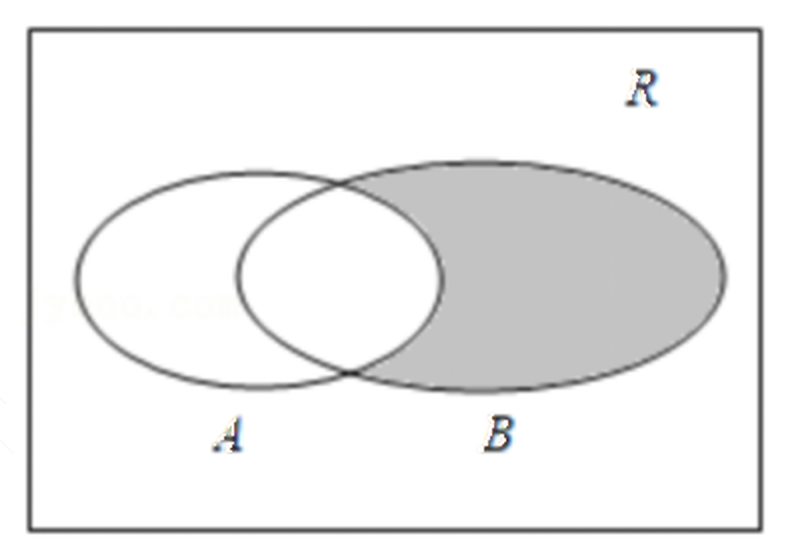
\includegraphics[width=0.36\textwidth]{figures/gao127_q4.png}
\end{center}

\ifanswer
\solbegin
\step{已知 $\R$ 是实数集，集合 $A=\{x\mid 1<x<2\}$, $B=\left\{x\mid 0<x<\frac32\right\}$,}
\step{阴影部分表示的集合是 $\overline A\cap B=\{x\mid 0<x\leqslant1\}$，即 $(0,1]$.}
\solend
\fi

\item 若集合 $\{x\mid (a-1)x^2+3x-2=0\}$ 有且仅有两个子集，则实数 $a$ 的值为\blankline[4.4em].

\ifanswer
\solbegin
\step{由题意得 $\{x\mid (a-1)x^2+3x-2=0\}$ 为单元素集，}
\step{所以 $a-1=0$ 或 $\begin{cases}a-1\neq0\\\triangle=9+8(a-1)=0\end{cases}$，所以 $a=1$ 或 $a=-\frac18$.}
\solend
\fi

\item 已知条件 $\alpha:x\leqslant m$，条件 $\beta:x^2-x\leqslant0$，若 $\alpha$ 是 $\beta$ 的必要条件，则实数 $m$ 的取值范围是为\blankline[4.4em].

\ifanswer
\solbegin
\step{不等式 $x^2-x\leqslant0$ 的解集为 $[0,1]$，}
\step{因为条件 $\alpha:x\leqslant m$，条件 $\beta:x^2-x\leqslant0$，且 $\alpha$ 是 $\beta$ 的必要条件，}
\step{所以集合 $[0,1]$ 是集合 $(-\infty,m]$ 的子集，得 $m\geqslant1$，实数 $m$ 的取值范围是 $[1,+\infty)$.}
\solend
\fi

\item 已知 $\alpha\in\{-2,-1,-\frac12,0,1,2\}$，若幂函数 $y=x^\alpha$ 在 $(0,+\infty)$ 是严格减函数且图像关于 $y$ 轴对称，则 $\alpha=$\blankline[4.4em].

\ifanswer
\solbegin
\step{幂函数 $y=x^\alpha$ 在 $(0,+\infty)$ 是严格减函数，则 $\alpha<0$，且图像关于 $y$ 轴对称，}
\step{则函数为偶函数，故 $\alpha=-2$.}
\solend
\fi

\item 若关于 $x$ 的不等式 $ax^2-3x+2<0$ 的解集不是空集，则实数 $a$ 的取值范围是\blankline[4.4em].

\ifanswer
\solbegin
\step{若 $a>0$，关于 $x$ 的不等式 $ax^2-3x+2<0$ 的解集不空，}
\step{所以一元二次方程 $ax^2-3x+2=0$ 的判别式大于零，}
\step{即 $(-3)^2-8a>0\Rightarrow a<\frac98$，结合 $a>0$ 得 $0<a<\frac98$；}
\step{若 $a\leqslant0$，则关于 $x$ 的不等式 $ax^2-3x+2<0$ 的解集不是空集；}
\step{综上，实数 $a$ 的取值范围是 $\left(-\infty,\frac98\right)$.}
\solend
\fi

\item 设 $\log_{18}2=a$，则 $\log_2 3$ 可用 $a$ 表示为\blankline[4.4em].

\ifanswer
\solbegin
\step{因为 $\log_{18}2=\frac{\log_2 2}{\log_2 18}=\frac1{1+2\log_2 3}=a$，则 $\log_2 3=\frac{1-a}{2a}$.}
\solend
\fi

\item 若关于 $x$ 的不等式 $ax^2+bx+c>0$ 解集为 $\left(-\frac12,3\right)$，则关于 $x$ 的不等式 $cx^2+bx+a<0$ 的解集为\blankline[4.4em].

\ifanswer
\solbegin
\step{由已知得 $a<0$，且 $ax^2+bx+c=a\left(x+\frac12\right)(x-3)$，}
\step{所以 $b=-\frac52 a, c=-\frac32 a$，}
\step{$cx^2+bx+a=-\frac a2(3x-1)(x+2)<0\Leftrightarrow(3x-1)(x+2)<0\Leftrightarrow -2<x<\frac13$，}
\step{故解集为 $\left(-2,\frac13\right)$.}
\solend
\fi

\item 设 $x\in\R$，则方程 $\lvert 2x+3\rvert-\lvert x-2\rvert=\lvert 3x+1\rvert$ 的解集为\blankline[4.4em].

\ifanswer
\solbegin
\step{当 $x\leqslant-\frac32$ 时，原式 $\Leftrightarrow -2x-3+x-2=-3x-1\Leftrightarrow x=2$，不合题意；}
\step{当 $-\frac32<x\leqslant-\frac13$ 时，原式 $\Leftrightarrow 2x+3+x-2=-3x-1\Leftrightarrow x=-\frac13$；}
\step{当 $-\frac13<x\leqslant2$ 时，原式 $\Leftrightarrow 2x+3+x-2=3x+1\Leftrightarrow 1=1$ 即恒成立；}
\step{当 $x>2$ 时，原式 $\Leftrightarrow 2x+3+2-x=3x+1\Leftrightarrow x=2$，不合题意；}
\step{故 $x\in\left[-\frac13,2\right]$.}
\solend
\fi

\item 若关于 $x$ 的不等式 $x^2-4mx+m<0$ 的解集为 $(x_1,x_2)$，若 $x_1>0,x_2>0$，试探究 $x_1+x_2,x_1x_2,x_1^2+x_2^2,\frac1{x_1}+\frac1{x_2}$ 的值，则 $4x_1+x_2$ 的最小值为\blankline[4.4em].

\ifanswer
\solbegin
\step{由题意得方程 $x^2-4mx+m=0$ 有两个相异的正实根 $x_1,x_2$，}
\step{故有 $\begin{cases}\triangle=16m^2-4m>0\\x_1+x_2=4m>0\\x_1\cdot x_2=m>0\end{cases}$，解得 $m>\frac14$，}
\step{则 $x_1^2+x_2^2=(x_1+x_2)^2-2x_1\cdot x_2=16m^2-2m$，$\frac1{x_1}+\frac1{x_2}=\frac{x_1+x_2}{x_1\cdot x_2}=4$，}
\step{则 $4x_1+x_2=\frac14(4x_1+x_2)\left(\frac1{x_1}+\frac1{x_2}\right)=\frac14\left(5+\frac{4x_1}{x_2}+\frac{x_2}{x_1}\right)\geqslant\frac94$，}
\step{当且仅当 $\frac{4x_1}{x_2}=\frac{x_2}{x_1}$ 时，即 $x_2=2x_1$ 时取等号，}
\step{由 $\begin{cases}x_2=2x_1\\\frac1{x_1}+\frac1{x_2}=4\end{cases}$，解得 $\begin{cases}x_1=\frac38\\x_2=\frac34\end{cases}$，于是 $m=x_1\cdot x_2=\frac9{32}\in\left(\frac14,+\infty\right)$，}
\step{即当 $m=\frac9{32}$ 时，$4x_1+x_2$ 取得最小值为 $\frac94$.}
\solend
\fi

\end{enumerate}

\bigsec{二、选择题}

\begin{enumerate}
\setcounter{enumi}{12}

\item 若 $a>0$, $a\neq1$, $M>0$, $N>0$，下列运算正确的是\mbox{（\quad）}

\keepwithprev
A. $\log_a\sqrt[N]{M}=\frac1N\log_a M$\qquad\qquad B. $(\log_a M)^N=N\log_a M$

C. $(\log_a M)\div(\log_a N)=\log_a(M-N)$\qquad\quad D. $\log_a M+\log_a N=\log_a(M+N)$

\ifanswer
\solbegin
\step{对于 $A$，$\log_a\sqrt[N]{M}=\log_a M^{\frac1N}=\frac1N\log_a M$，故 $A$ 正确；}
\step{对于 $B$，$(\log_a M)^N\neq N\log_a M=log_a M^n$，故 $B$ 错误；}
\step{对于 $C$，$(\log_a M)\div(\log_a N)\neq\log_a(M-N)$，故 $C$ 错误；}
\step{对于 $D$，$\log_a M+\log_a N=\log_a MN\neq\log_a(M+N)$，故 $D$ 错误.}
\step{故选 $A$.}
\solend
\fi

\item 下列不等式中正确的是\mbox{（\quad）}

\keepwithprev
A. 若 $a>b$，则 $ac^2>bc^2$\qquad\qquad B. 若 $a<b<0$，则 $a^2<b^2$

C. 若 $1<a<2$ 且 $0<b<3$，则 $1<a+b<5$\qquad D. 若 $\frac1a<1$，则 $a>1$

\ifanswer
\solbegin
\step{$C$ 中 $1+0<a+b<2+3$，即 $1<a+b<5$，正确.}
\step{$A$ 取 $c=0$ 时不成立；$B$ 应为 $a^2>b^2$；$D$ 取 $a=-1$ 时不成立. 故选 $C$.}
\solend
\fi

\item 已知 $y_1=x^3,y_2=x^2$，则下列说法正确的是\mbox{（\quad）}

\keepwithprev
A. $x\in(0,+\infty)$ 时，恒有 $y_1\geqslant y_2$

B. $y_1=x^3$ 与 $y_2=x^2$ 的函数图象仅有唯一交点

C. $x\in(0,1)$ 时，$y_1=x^3$ 图象在 $y_2=x^2$ 图象下方

D. 存在 $x_0\in(1,+\infty)$ 使得 $y_1=y_2$

\ifanswer
\solbegin
\step{$y_1-y_2=x^2(x-1)$，当 $0<x<1$ 时，$y_1<y_2$，故 $C$ 正确，$A$ 错误.}
\step{$y_1=y_2\Leftrightarrow x^2(x-1)=0\Leftrightarrow x=0$ 或 $x=1$，两图象有两个交点，故 $BD$ 错误.}
\step{故选 $C$.}
\solend
\fi

\item 已知非空集合 $A$、$B$ 满足两个条件：(1) $A\cup B=\{1,2,3,4,5,6,7\}$, $A\cap B=\varnothing$；(2) 若 $x\in A$，则 $x+1\in B$，则有序集合对 $(A,B)$ 的个数为\mbox{（\quad）}

\keepwithprev
A. $17$\qquad\qquad B. $18$\qquad\qquad C. $19$\qquad\qquad D. $20$

\ifanswer
\solbegin
\step{当 $A$ 为单元素集合时，有 6 种情况：}
\step{当 $A$ 为双元素集合时，$A=\{1,3\}, A=\{1,4\}, A=\{1,5\}, A=\{1,6\}, A=\{2,4\}$,}
\step{$A=\{2,5\}, A=\{2,6\}, A=\{3,5\}, A=\{3,6\}, A=\{4,6\}$，共 10 种情况；}
\step{当 $A$ 为三元素集合时，$A=\{1,3,5\}, A=\{1,3,6\}, A=\{1,4,6\}, A=\{2,4,6\}$，}
\step{共 4 种情况；}
\step{当 $A$ 为四元素集合时，不成立；}
\step{故有序集合对 $(A,B)$ 的个数为 20，故选 $D$.}
\solend
\fi

\end{enumerate}

\bigsec{三、解答题}

\begin{enumerate}
\setcounter{enumi}{16}

\item 已知 $x,y\in\R$，比较 $x^2+y^2$ 与 $2(2x-y)-5$ 的大小.

\ifanswer
\solbegin
\step{因为 $x^2+y^2-2(2x-y)+5=(x-2)^2+(y+1)^2\geqslant0$，}
\step{所以 $x^2+y^2\geqslant2(2x-y)-5$.}
\solend
\fi

\item 已知集合 $A=\{x\mid x^2+4x=0\}$，$B=\{x\mid x^2+2(a+1)x+a^2-1=0\}$.

(1) 若 $A$ 是 $B$ 的子集，求实数 $a$ 的值；

(2) 若 $B$ 是 $A$ 的子集，求实数 $a$ 的取值范围.

\ifanswer
\solbegin
\step{(1) 因为 $A=\{-4,0\}$，$B=\{x\mid x^2+2(a+1)x+a^2-1=0\}$，又 $A\subseteq B$，}
\step{所以 $A=B$，所以 $\begin{cases}-4+0=-2(a+1)\\-4\times0=a^2-1\end{cases}$，所以 $a=1$；}
\step{(2) 因为 $B$ 是 $A$ 的子集，所以 $B=\varnothing$ 或 $B=\{-4\}$ 或 $B=\{0\}$ 或 $B=\{-4,0\}$，}
\step{① $B=\varnothing$ 时，$\triangle=4(a+1)^2-4(a^2-1)<0$，所以 $a<-1$；}
\step{② $B=\{-4\}$ 时，$\begin{cases}-4+(-4)=-2(a+1)\\-4\times(-4)=a^2-1\end{cases}$，无解；}
\step{③ $B=\{0\}$ 时，$\begin{cases}0+0=-2(a+1)\\0\times0=a^2-1\end{cases}$，所以 $a=-1$；}
\step{④ $B=\{-4,0\}$ 时，由 (1) 得 $a=1$，}
\step{综上，实数 $a$ 的取值范围为 $(-\infty,-1]\cup\{1\}$.}
\solend
\fi

\item 某企业在现有设备下每日生产原先成本 $y$（单位：万元）与日产量 $x$（单位：吨）之间的函数关系式：$y=2x^2+(15-4k)x+120k+8$，近年来各部门都非常重视大气污染防治工作，为了配合环境卫生综合整治，该企业引进了除尘设备，每吨产品的除尘费用为 $k$ 万元，引进除尘设备后，当日产量 $x=1$ 时，总成本（总成本为原先成本和除尘费用之和）为 142 万元.

(1) 求 $k$ 的值；

(2) 求引进除尘设备后日产量为多少时，每吨产品的成本最小，并求出最小值.

\ifanswer
\solbegin
\step{(1) 该企业引进了除尘设备，}
\step{每日生产总成本 $h$（单位：万元）与日产量 $x$（单位：吨）之间的关系为}
\step{$h=2x^2+(15-4k)x+120k+8+kx=2x^2+(15-3k)x+120k+8$，}
\step{当日产量 $x=1$ 时，总成本为 $h=142$ 万元，}
\step{代入得 $2+(15-3k)+120k+8=142\Rightarrow k=1$，}
\step{(2) 由 (1) 得 $h=2x^2+12x+128$，}
\step{所以每吨产品的成本为 $w=\frac{2x^2+12x+128}{x}=2x+\frac{128}{x}+12$}
\step{$\geqslant2\sqrt{2x\cdot\frac{128}{x}}+12=44$，当且仅当 $2x=\frac{128}{x}$，即 $x=8$ 时，取等号，}
\step{所以引进除尘设备后日产量为 8 吨时，每吨产品的成本最小，}
\step{且最小值为 44 万元.}
\solend
\fi

\item 已知集合 $A=\{x\mid \lvert x-a\rvert<2\}$，集合 $B=\left\{x\mid\frac{2x-1}{x+2}<1\right\}$.

(1) 若 $a=2$，求 $A\cup B$；

(2) 若 $A\cap B=A$，求实数 $a$ 的取值范围.

\ifanswer
\solbegin
\step{(1) 若 $a=2$，则 $A=\{x\mid \lvert x-a\rvert<2\}=\{x\mid \lvert x-2\rvert<2\}=\{x\mid 0<x<4\}$，}
\step{由 $\frac{2x-1}{x+2}<1$ 得 $\frac{x-3}{x+2}<0$，即 $(x-3)(x+2)<0$，解得 $-2<x<3$，}
\step{所以 $B=\{x\mid -2<x<3\}$，所以 $A\cup B=\{x\mid -2<x<4\}$；}
\step{(2) 由 (1) 得 $B=\{x\mid -2<x<3\}$，}
\step{$A=\{x\mid \lvert x-a\rvert<2\}=\{x\mid a-2<x<a+2\}$，}
\step{若 $A\cap B=A$，则 $A\subseteq B$，则 $\begin{cases}a-2\geqslant-2\\a+2\leqslant3\end{cases}$，解得 $0\leqslant a\leqslant1$，}
\step{即实数 $a$ 的取值范围为 $[0,1]$.}
\solend
\fi

\item 已知自变量为 $x$ 的函数 $y=\frac{ax+b}{x+a}$，

(1) 若 $a=1$ 且 $b=2$，则函数 $y=\frac{ax+b}{x+a}$ 图像可由幂函数\blankline[4.4em]（写解析式）先沿 $x$ 轴方向\blankline[4.4em]平移\blankline[4.4em]个单位，再沿 $y$ 轴方向向上平移\blankline[4.4em]个单位得到；

(2) 当 $a>0$ 且 $b=-2$ 时不等式 $\frac{ax+b}{x+a}\leqslant\frac{2x^2}{x+a}$ 对 $x>0$ 恒成立，求实数 $a$ 的最大值；

(3) 若 $b=-2$ 且关于 $x$ 的不等式 $x^2\log_2\frac{4(a+1)}a+2x\log_2\frac{2a}{a+1}+\log_2\frac{(a+1)^2}{4a^2}\leqslant0$ 解集是单元素集，求出 $a$ 值，并求出函数 $y=\frac{ax-2}{x+a}$ 的对称中心.

\ifanswer
\solbegin
\step{(1) 已知自变量为 $x$ 的函数 $y=\frac{ax+b}{x+a}$，}
\step{当 $a=1$ 且 $b=2$ 时，$y=\frac{x+2}{x+1}=\frac{x+1+1}{x+1}=1+\frac1{x+1}$，}
\step{由幂函数 $y=\frac1x$，先沿 $x$ 轴方向向左平移一个单位，}
\step{再沿 $y$ 轴方向向上平移一个单位得到；}
\step{(2) 当 $a>0$ 且 $b=-2$ 时不等式 $\frac{ax+b}{x+a}\leqslant\frac{2x^2}{x+a}$ 即 $\frac{ax-2}{x+a}\leqslant\frac{2x^2}{x+a}$ 对 $x>0$ 恒成立，}
\step{因为 $a>0$ 且 $x>0$，所以 $x+a>0$，所以等价于 $ax-2\leqslant2x^2$ 对 $x>0$ 恒成立，}
\step{即 $2x^2-ax+2\geqslant0$ 对 $x>0$ 恒成立，}
\step{因为函数 $g(x)=2x^2-ax+2$ 的对称轴 $x=\frac a4>0$，且 $g(0)=2>0$，}
\step{则 $\begin{cases}\triangle=(-a)^2-4\times2\times2\leqslant0\\a>0\end{cases}$，解得 $0<a\leqslant4$，所以 $a$ 的最大值为 4；}
\step{(3) 关于 $x$ 的不等式 $x^2\log_2\frac{4(a+1)}a+2x\log_2\frac{2a}{a+1}+\log_2\frac{(a+1)^2}{4a^2}\leqslant0$ 解集}
\step{是单元素集，由 $\frac{4(a+1)}a>0$，则 $a>0$ 或 $a<-1$，}
\step{若 $\log_2\frac{4(a+1)}a=0$，则 $\frac{4(a+1)}a=1$，解得 $a=-\frac43$，}
\step{此时不等式为 $6x-6\leqslant0$，解得 $x\leqslant1$，不符合题意，}
\step{若 $\log_2\frac{4(a+1)}a>0$，即 $\frac{4(a+1)}a>1$，解得 $a>0$ 或 $a<-\frac43$，}
\step{则 $\triangle=\left(2\log_2\frac{2a}{a+1}\right)^2-4\log_2\frac{4(a+1)}a\cdot\log_2\frac{(a+1)^2}{4a^2}=0$，}
\step{令 $\log_2\frac{2a}{a+1}=t$，则 $t^2-(3-t)(-2t)=0$，解得 $t=0$ 或 $t=6$，}
\step{当 $\log_2\frac{2a}{a+1}=0$，解得 $a=1$，$\log_2\frac{2a}{a+1}=6$，解得 $a=-\frac{32}{31}$(舍去)，所以 $a=1$，}
\step{则函数 $y=\frac{ax-2}{x+a}$ 即为 $y=\frac{x-2}{x+1}=\frac{x+1-3}{x+1}=1+\frac{-3}{x+1}$，}
\step{对称中心为 $(-1,1)$.}
\solend
\fi

\end{enumerate}

\end{document}
"
%
% 原始材料：微信公众号“魔都数学加油站”文章，作者破晓，2026-11-11 18:35 发布；
% 连载“27学年高一127”，原文标题“27学年高一127——2026-2027年上海市南汇一中高一上期中”；
% 原文链接：https://mp.weixin.qq.com/s/nozIwRgeWSKPCPSiqfCm2Q。
% 正文为 9 张 PNG 页（01、02、03、09 为 2560×3620，04、05、06、07、08 为 4762×6735），
% 题目下印有【解析】，为讲评版。题目、解析均据原图转录；
% 卷面粉红色水印“魔都数学加油站”及公众号页脚未录入。全卷仅第 4 题一幅插图。
% 第 09 页只有一行“对称中心为(-1,1).”及水印，是第 08 页末行的续尾页。
%
% 卷首标题：原卷印作“2026-2027 年南汇一中高一上期中”（公众号标题中的“上海市”
% 卷面标题行没有，本稿照卷面），年份区间按全稿惯例排 en dash；原卷未印副标题，
% 本卷为期中卷、跨三章，按题目内容标为“集合与常用逻辑用语、不等式、函数”
% （第 4/5/6/16/18/20 题为集合与常用逻辑用语，第 8/10/11/12/14/17 题为不等式，
% 第 3/7/9/13/15/19/21 题为函数；与 106、125 同为期中复习卷，口径相同）。
%
% 与原卷的排版差异：
%   ① 原文从第 3 题起，填空题编号为 3—12、选择题为 13—16、解答题为 17—21，本稿保留原题号；
%   ② 原卷每题下直接印【解析】，本稿按全稿惯例置于答案版；四道选择题答案均在解析末句
%      “故选 …”，括号内留空、不另提 \ans{}；全卷无只印【答案】或括号内答案的题；
%   ③ 原卷未印副标题，本稿按“知识模块”口径补出；
%   ④ 原卷填空横线按全稿惯例排为 \blankline[4.4em]；选择题括号排 \mbox{（\quad）}、
%      选项段前按惯例加 \keepwithprev；解答题不留作答区（原卷为讲评版，与 109—125 同）；
%      第 21 题 (1) 的四处填空横线亦排 \blankline[4.4em]；
%   ⑤ 原卷数集排斜体 $R$，按全稿惯例改 \R；绝对值排 \lvert…\rvert，集合描述竖线排 \mid；
%      补集记号照原卷上划线排 \overline{A}；不等号一律 \leqslant / \geqslant；
%   ⑥ 第 4 题插图原在题干右侧，本稿按全稿惯例移至题干之后居中排（取原卷截图、
%      去粉色水印后 2× LANCZOS 放大，存 figures/gao127_q4.png），三版都出；
%      并在该题 \item 前加 \needvspace{} 守卫，把题干与插图整块推走；
%   ⑦ 原卷子题编号 (1)(2)(3) 与括号按全稿惯例排；“（单位：万元）”“（写解析式）”
%      用全角括号，第 21 题 (3) 解析“(舍去)”用半角括号，均照录；
%   ⑧ 第 09 页仅一行“对称中心为(-1,1).”为第 08 页末行之续尾，本稿按原卷印刷行
%      另起一条 \step，置于答案版最后一题解析之末。
%
% 子集符号：第 18 题 (1) 解析 $A\subseteq B$、第 20 题 (2) 解析 $A\subseteq B$ 均印有
%   下划线，照录 \subseteq；全卷无 \subset。回原图放大逐处确认。
%
% 判别式字形：本卷 5 处判别式（第 5 题解析 cases 内 $\triangle=9+8(a-1)=0$、
%   第 12 题解析 cases 内 $\triangle=16m^2-4m>0$、第 18 题① $\triangle=4(a+1)^2-4(a^2-1)<0$、
%   第 21 题 (2) cases 内 $\triangle=(-a)^2-4\times2\times2\leqslant0$、
%   第 21 题 (3) $\triangle=\left(2\log_2\frac{2a}{a+1}\right)^2-\cdots=0$）均排等边扁三角，
%   照录 \triangle；逐处回原图全分辨率放大确认，无高三角 $\Delta$（与 高一26 排 $\Delta$ 不同）。
%
% 原卷存疑照录：
%   第 6 题题干作“则实数 $m$ 的取值范围是为____”（“是为”叠用，疑衍一字），照录；
%   第 12 题题干“试探究 $x_1+x_2, x_1x_2, x_1^2+x_2^2, \frac1{x_1}+\frac1{x_2}$ 的值，
%     则 $4x_1+x_2$ 的最小值为____”与后文衔接突兀，照录；
%   第 13 题解析 B 作“$(\log_a M)^N\neq N\log_a M=log_a M^n$”，后一 log 为斜体、
%     指数作小写 $n$，与前式 $N\log_a M$ 及题干 $N$ 不一致，照录；
%   第 13 题解析 A、B、C 三步句末用“；”，D 步句末用“.”，标点不一致，照录；
%   第 15 题解析“故 $BD$ 错误.”两选项字母连写、无顿号，照录；
%   第 7 题题干及解析用“图像”，第 15 题 B、C 及解析用“图象”，全卷两种写法混用，照录未统一；
%   第 21 题 (3) 题干“求出 $a$ 值”（通常作“求出 $a$ 的值”），照录；
%   第 21 题 (3) 解析“解得 $a=1$，$\log_2\frac{2a}{a+1}=6$，解得 $a=-\frac{32}{31}$(舍去)，
%     所以 $a=1$”两个“解得”并列、且舍去值用半角括号，照录；
%   第 09 页“对称中心为(-1,1).”用半角括号与半角句点，照录；
%   第 8 题解析“若 $a\leqslant0$，则关于 $x$ 的不等式 $ax^2-3x+2<0$ 的解集不是空集；”
%     未给理由直接断言，照录；
%   第 18 题 (1) 由 $A\subseteq B$ 直接得 $A=B$，照录。
%
% 行数核对：逐题数 \step 条数，合计 95 条（Q3：1；Q4：2；Q5：2；Q6：3；Q7：2；
% Q8：5；Q9：1；Q10：4；Q11：5；Q12：7；Q13：5；Q14：2；Q15：3；Q16：7；
% Q17：2；Q18：8；Q19：10；Q20：7；Q21：19），与原卷印刷行逐题相等
% （cases 块作一个印刷行计；Q21 第 19 行为第 09 页续尾）。全卷 19 题均印【解析】，
% 无只印【答案】或括号内答案的题，故 \ans{} 为 0；四道选择题括号内留空、不另提 \ans{}。
%
\documentclass[a4paper,11pt]{article}
\usepackage{common}

\begin{document}

\examtitlest[3]{2026--2027 年南汇一中高一上期中}{集合与常用逻辑用语、不等式、函数}

\bigsec{一、填空题}

\begin{enumerate}
\setcounter{enumi}{2}

\item 把 $\sqrt[4]{a\sqrt a}(a>0)$ 化成有理数指数幂的形式为\blankline[4.4em].

\ifanswer
\solbegin
\step{$\sqrt[4]{a\sqrt a}=(a\cdot a^{\frac12})^{\frac14}=a^{\frac38}$.}
\solend
\fi

\needvspace{6.5cm}
\item 已知集合 $A=\{x\mid 1<x<2\}$, $B=\left\{x\mid 0<x<\frac32\right\}$, 则如图阴影部分表示的集合是\blankline[4.4em].

\begin{center}
% 图取原卷截图（第 1 页题干右侧）、去水印后 2× LANCZOS 放大，本稿移至题干之后
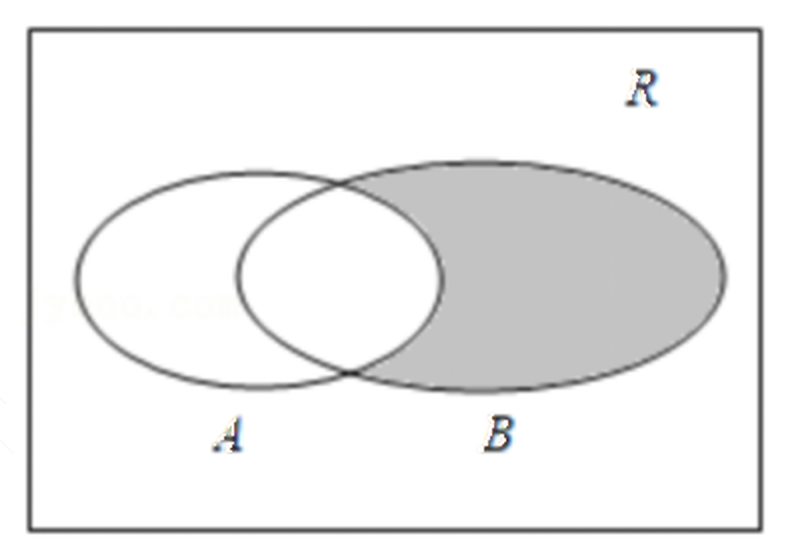
\includegraphics[width=0.36\textwidth]{figures/gao127_q4.png}
\end{center}

\ifanswer
\solbegin
\step{已知 $\R$ 是实数集，集合 $A=\{x\mid 1<x<2\}$, $B=\left\{x\mid 0<x<\frac32\right\}$,}
\step{阴影部分表示的集合是 $\overline A\cap B=\{x\mid 0<x\leqslant1\}$，即 $(0,1]$.}
\solend
\fi

\item 若集合 $\{x\mid (a-1)x^2+3x-2=0\}$ 有且仅有两个子集，则实数 $a$ 的值为\blankline[4.4em].

\ifanswer
\solbegin
\step{由题意得 $\{x\mid (a-1)x^2+3x-2=0\}$ 为单元素集，}
\step{所以 $a-1=0$ 或 $\begin{cases}a-1\neq0\\\triangle=9+8(a-1)=0\end{cases}$，所以 $a=1$ 或 $a=-\frac18$.}
\solend
\fi

\item 已知条件 $\alpha:x\leqslant m$，条件 $\beta:x^2-x\leqslant0$，若 $\alpha$ 是 $\beta$ 的必要条件，则实数 $m$ 的取值范围是为\blankline[4.4em].

\ifanswer
\solbegin
\step{不等式 $x^2-x\leqslant0$ 的解集为 $[0,1]$，}
\step{因为条件 $\alpha:x\leqslant m$，条件 $\beta:x^2-x\leqslant0$，且 $\alpha$ 是 $\beta$ 的必要条件，}
\step{所以集合 $[0,1]$ 是集合 $(-\infty,m]$ 的子集，得 $m\geqslant1$，实数 $m$ 的取值范围是 $[1,+\infty)$.}
\solend
\fi

\item 已知 $\alpha\in\{-2,-1,-\frac12,0,1,2\}$，若幂函数 $y=x^\alpha$ 在 $(0,+\infty)$ 是严格减函数且图像关于 $y$ 轴对称，则 $\alpha=$\blankline[4.4em].

\ifanswer
\solbegin
\step{幂函数 $y=x^\alpha$ 在 $(0,+\infty)$ 是严格减函数，则 $\alpha<0$，且图像关于 $y$ 轴对称，}
\step{则函数为偶函数，故 $\alpha=-2$.}
\solend
\fi

\item 若关于 $x$ 的不等式 $ax^2-3x+2<0$ 的解集不是空集，则实数 $a$ 的取值范围是\blankline[4.4em].

\ifanswer
\solbegin
\step{若 $a>0$，关于 $x$ 的不等式 $ax^2-3x+2<0$ 的解集不空，}
\step{所以一元二次方程 $ax^2-3x+2=0$ 的判别式大于零，}
\step{即 $(-3)^2-8a>0\Rightarrow a<\frac98$，结合 $a>0$ 得 $0<a<\frac98$；}
\step{若 $a\leqslant0$，则关于 $x$ 的不等式 $ax^2-3x+2<0$ 的解集不是空集；}
\step{综上，实数 $a$ 的取值范围是 $\left(-\infty,\frac98\right)$.}
\solend
\fi

\item 设 $\log_{18}2=a$，则 $\log_2 3$ 可用 $a$ 表示为\blankline[4.4em].

\ifanswer
\solbegin
\step{因为 $\log_{18}2=\frac{\log_2 2}{\log_2 18}=\frac1{1+2\log_2 3}=a$，则 $\log_2 3=\frac{1-a}{2a}$.}
\solend
\fi

\item 若关于 $x$ 的不等式 $ax^2+bx+c>0$ 解集为 $\left(-\frac12,3\right)$，则关于 $x$ 的不等式 $cx^2+bx+a<0$ 的解集为\blankline[4.4em].

\ifanswer
\solbegin
\step{由已知得 $a<0$，且 $ax^2+bx+c=a\left(x+\frac12\right)(x-3)$，}
\step{所以 $b=-\frac52 a, c=-\frac32 a$，}
\step{$cx^2+bx+a=-\frac a2(3x-1)(x+2)<0\Leftrightarrow(3x-1)(x+2)<0\Leftrightarrow -2<x<\frac13$，}
\step{故解集为 $\left(-2,\frac13\right)$.}
\solend
\fi

\item 设 $x\in\R$，则方程 $\lvert 2x+3\rvert-\lvert x-2\rvert=\lvert 3x+1\rvert$ 的解集为\blankline[4.4em].

\ifanswer
\solbegin
\step{当 $x\leqslant-\frac32$ 时，原式 $\Leftrightarrow -2x-3+x-2=-3x-1\Leftrightarrow x=2$，不合题意；}
\step{当 $-\frac32<x\leqslant-\frac13$ 时，原式 $\Leftrightarrow 2x+3+x-2=-3x-1\Leftrightarrow x=-\frac13$；}
\step{当 $-\frac13<x\leqslant2$ 时，原式 $\Leftrightarrow 2x+3+x-2=3x+1\Leftrightarrow 1=1$ 即恒成立；}
\step{当 $x>2$ 时，原式 $\Leftrightarrow 2x+3+2-x=3x+1\Leftrightarrow x=2$，不合题意；}
\step{故 $x\in\left[-\frac13,2\right]$.}
\solend
\fi

\item 若关于 $x$ 的不等式 $x^2-4mx+m<0$ 的解集为 $(x_1,x_2)$，若 $x_1>0,x_2>0$，试探究 $x_1+x_2,x_1x_2,x_1^2+x_2^2,\frac1{x_1}+\frac1{x_2}$ 的值，则 $4x_1+x_2$ 的最小值为\blankline[4.4em].

\ifanswer
\solbegin
\step{由题意得方程 $x^2-4mx+m=0$ 有两个相异的正实根 $x_1,x_2$，}
\step{故有 $\begin{cases}\triangle=16m^2-4m>0\\x_1+x_2=4m>0\\x_1\cdot x_2=m>0\end{cases}$，解得 $m>\frac14$，}
\step{则 $x_1^2+x_2^2=(x_1+x_2)^2-2x_1\cdot x_2=16m^2-2m$，$\frac1{x_1}+\frac1{x_2}=\frac{x_1+x_2}{x_1\cdot x_2}=4$，}
\step{则 $4x_1+x_2=\frac14(4x_1+x_2)\left(\frac1{x_1}+\frac1{x_2}\right)=\frac14\left(5+\frac{4x_1}{x_2}+\frac{x_2}{x_1}\right)\geqslant\frac94$，}
\step{当且仅当 $\frac{4x_1}{x_2}=\frac{x_2}{x_1}$ 时，即 $x_2=2x_1$ 时取等号，}
\step{由 $\begin{cases}x_2=2x_1\\\frac1{x_1}+\frac1{x_2}=4\end{cases}$，解得 $\begin{cases}x_1=\frac38\\x_2=\frac34\end{cases}$，于是 $m=x_1\cdot x_2=\frac9{32}\in\left(\frac14,+\infty\right)$，}
\step{即当 $m=\frac9{32}$ 时，$4x_1+x_2$ 取得最小值为 $\frac94$.}
\solend
\fi

\end{enumerate}

\bigsec{二、选择题}

\begin{enumerate}
\setcounter{enumi}{12}

\item 若 $a>0$, $a\neq1$, $M>0$, $N>0$，下列运算正确的是\mbox{（\quad）}

\keepwithprev
A. $\log_a\sqrt[N]{M}=\frac1N\log_a M$\qquad\qquad B. $(\log_a M)^N=N\log_a M$

C. $(\log_a M)\div(\log_a N)=\log_a(M-N)$\qquad\quad D. $\log_a M+\log_a N=\log_a(M+N)$

\ifanswer
\solbegin
\step{对于 $A$，$\log_a\sqrt[N]{M}=\log_a M^{\frac1N}=\frac1N\log_a M$，故 $A$ 正确；}
\step{对于 $B$，$(\log_a M)^N\neq N\log_a M=log_a M^n$，故 $B$ 错误；}
\step{对于 $C$，$(\log_a M)\div(\log_a N)\neq\log_a(M-N)$，故 $C$ 错误；}
\step{对于 $D$，$\log_a M+\log_a N=\log_a MN\neq\log_a(M+N)$，故 $D$ 错误.}
\step{故选 $A$.}
\solend
\fi

\item 下列不等式中正确的是\mbox{（\quad）}

\keepwithprev
A. 若 $a>b$，则 $ac^2>bc^2$\qquad\qquad B. 若 $a<b<0$，则 $a^2<b^2$

C. 若 $1<a<2$ 且 $0<b<3$，则 $1<a+b<5$\qquad D. 若 $\frac1a<1$，则 $a>1$

\ifanswer
\solbegin
\step{$C$ 中 $1+0<a+b<2+3$，即 $1<a+b<5$，正确.}
\step{$A$ 取 $c=0$ 时不成立；$B$ 应为 $a^2>b^2$；$D$ 取 $a=-1$ 时不成立. 故选 $C$.}
\solend
\fi

\item 已知 $y_1=x^3,y_2=x^2$，则下列说法正确的是\mbox{（\quad）}

\keepwithprev
A. $x\in(0,+\infty)$ 时，恒有 $y_1\geqslant y_2$

B. $y_1=x^3$ 与 $y_2=x^2$ 的函数图象仅有唯一交点

C. $x\in(0,1)$ 时，$y_1=x^3$ 图象在 $y_2=x^2$ 图象下方

D. 存在 $x_0\in(1,+\infty)$ 使得 $y_1=y_2$

\ifanswer
\solbegin
\step{$y_1-y_2=x^2(x-1)$，当 $0<x<1$ 时，$y_1<y_2$，故 $C$ 正确，$A$ 错误.}
\step{$y_1=y_2\Leftrightarrow x^2(x-1)=0\Leftrightarrow x=0$ 或 $x=1$，两图象有两个交点，故 $BD$ 错误.}
\step{故选 $C$.}
\solend
\fi

\item 已知非空集合 $A$、$B$ 满足两个条件：(1) $A\cup B=\{1,2,3,4,5,6,7\}$, $A\cap B=\varnothing$；(2) 若 $x\in A$，则 $x+1\in B$，则有序集合对 $(A,B)$ 的个数为\mbox{（\quad）}

\keepwithprev
A. $17$\qquad\qquad B. $18$\qquad\qquad C. $19$\qquad\qquad D. $20$

\ifanswer
\solbegin
\step{当 $A$ 为单元素集合时，有 6 种情况：}
\step{当 $A$ 为双元素集合时，$A=\{1,3\}, A=\{1,4\}, A=\{1,5\}, A=\{1,6\}, A=\{2,4\}$,}
\step{$A=\{2,5\}, A=\{2,6\}, A=\{3,5\}, A=\{3,6\}, A=\{4,6\}$，共 10 种情况；}
\step{当 $A$ 为三元素集合时，$A=\{1,3,5\}, A=\{1,3,6\}, A=\{1,4,6\}, A=\{2,4,6\}$，}
\step{共 4 种情况；}
\step{当 $A$ 为四元素集合时，不成立；}
\step{故有序集合对 $(A,B)$ 的个数为 20，故选 $D$.}
\solend
\fi

\end{enumerate}

\bigsec{三、解答题}

\begin{enumerate}
\setcounter{enumi}{16}

\item 已知 $x,y\in\R$，比较 $x^2+y^2$ 与 $2(2x-y)-5$ 的大小.

\ifanswer
\solbegin
\step{因为 $x^2+y^2-2(2x-y)+5=(x-2)^2+(y+1)^2\geqslant0$，}
\step{所以 $x^2+y^2\geqslant2(2x-y)-5$.}
\solend
\fi

\item 已知集合 $A=\{x\mid x^2+4x=0\}$，$B=\{x\mid x^2+2(a+1)x+a^2-1=0\}$.

(1) 若 $A$ 是 $B$ 的子集，求实数 $a$ 的值；

(2) 若 $B$ 是 $A$ 的子集，求实数 $a$ 的取值范围.

\ifanswer
\solbegin
\step{(1) 因为 $A=\{-4,0\}$，$B=\{x\mid x^2+2(a+1)x+a^2-1=0\}$，又 $A\subseteq B$，}
\step{所以 $A=B$，所以 $\begin{cases}-4+0=-2(a+1)\\-4\times0=a^2-1\end{cases}$，所以 $a=1$；}
\step{(2) 因为 $B$ 是 $A$ 的子集，所以 $B=\varnothing$ 或 $B=\{-4\}$ 或 $B=\{0\}$ 或 $B=\{-4,0\}$，}
\step{① $B=\varnothing$ 时，$\triangle=4(a+1)^2-4(a^2-1)<0$，所以 $a<-1$；}
\step{② $B=\{-4\}$ 时，$\begin{cases}-4+(-4)=-2(a+1)\\-4\times(-4)=a^2-1\end{cases}$，无解；}
\step{③ $B=\{0\}$ 时，$\begin{cases}0+0=-2(a+1)\\0\times0=a^2-1\end{cases}$，所以 $a=-1$；}
\step{④ $B=\{-4,0\}$ 时，由 (1) 得 $a=1$，}
\step{综上，实数 $a$ 的取值范围为 $(-\infty,-1]\cup\{1\}$.}
\solend
\fi

\item 某企业在现有设备下每日生产原先成本 $y$（单位：万元）与日产量 $x$（单位：吨）之间的函数关系式：$y=2x^2+(15-4k)x+120k+8$，近年来各部门都非常重视大气污染防治工作，为了配合环境卫生综合整治，该企业引进了除尘设备，每吨产品的除尘费用为 $k$ 万元，引进除尘设备后，当日产量 $x=1$ 时，总成本（总成本为原先成本和除尘费用之和）为 142 万元.

(1) 求 $k$ 的值；

(2) 求引进除尘设备后日产量为多少时，每吨产品的成本最小，并求出最小值.

\ifanswer
\solbegin
\step{(1) 该企业引进了除尘设备，}
\step{每日生产总成本 $h$（单位：万元）与日产量 $x$（单位：吨）之间的关系为}
\step{$h=2x^2+(15-4k)x+120k+8+kx=2x^2+(15-3k)x+120k+8$，}
\step{当日产量 $x=1$ 时，总成本为 $h=142$ 万元，}
\step{代入得 $2+(15-3k)+120k+8=142\Rightarrow k=1$，}
\step{(2) 由 (1) 得 $h=2x^2+12x+128$，}
\step{所以每吨产品的成本为 $w=\frac{2x^2+12x+128}{x}=2x+\frac{128}{x}+12$}
\step{$\geqslant2\sqrt{2x\cdot\frac{128}{x}}+12=44$，当且仅当 $2x=\frac{128}{x}$，即 $x=8$ 时，取等号，}
\step{所以引进除尘设备后日产量为 8 吨时，每吨产品的成本最小，}
\step{且最小值为 44 万元.}
\solend
\fi

\item 已知集合 $A=\{x\mid \lvert x-a\rvert<2\}$，集合 $B=\left\{x\mid\frac{2x-1}{x+2}<1\right\}$.

(1) 若 $a=2$，求 $A\cup B$；

(2) 若 $A\cap B=A$，求实数 $a$ 的取值范围.

\ifanswer
\solbegin
\step{(1) 若 $a=2$，则 $A=\{x\mid \lvert x-a\rvert<2\}=\{x\mid \lvert x-2\rvert<2\}=\{x\mid 0<x<4\}$，}
\step{由 $\frac{2x-1}{x+2}<1$ 得 $\frac{x-3}{x+2}<0$，即 $(x-3)(x+2)<0$，解得 $-2<x<3$，}
\step{所以 $B=\{x\mid -2<x<3\}$，所以 $A\cup B=\{x\mid -2<x<4\}$；}
\step{(2) 由 (1) 得 $B=\{x\mid -2<x<3\}$，}
\step{$A=\{x\mid \lvert x-a\rvert<2\}=\{x\mid a-2<x<a+2\}$，}
\step{若 $A\cap B=A$，则 $A\subseteq B$，则 $\begin{cases}a-2\geqslant-2\\a+2\leqslant3\end{cases}$，解得 $0\leqslant a\leqslant1$，}
\step{即实数 $a$ 的取值范围为 $[0,1]$.}
\solend
\fi

\item 已知自变量为 $x$ 的函数 $y=\frac{ax+b}{x+a}$，

(1) 若 $a=1$ 且 $b=2$，则函数 $y=\frac{ax+b}{x+a}$ 图像可由幂函数\blankline[4.4em]（写解析式）先沿 $x$ 轴方向\blankline[4.4em]平移\blankline[4.4em]个单位，再沿 $y$ 轴方向向上平移\blankline[4.4em]个单位得到；

(2) 当 $a>0$ 且 $b=-2$ 时不等式 $\frac{ax+b}{x+a}\leqslant\frac{2x^2}{x+a}$ 对 $x>0$ 恒成立，求实数 $a$ 的最大值；

(3) 若 $b=-2$ 且关于 $x$ 的不等式 $x^2\log_2\frac{4(a+1)}a+2x\log_2\frac{2a}{a+1}+\log_2\frac{(a+1)^2}{4a^2}\leqslant0$ 解集是单元素集，求出 $a$ 值，并求出函数 $y=\frac{ax-2}{x+a}$ 的对称中心.

\ifanswer
\solbegin
\step{(1) 已知自变量为 $x$ 的函数 $y=\frac{ax+b}{x+a}$，}
\step{当 $a=1$ 且 $b=2$ 时，$y=\frac{x+2}{x+1}=\frac{x+1+1}{x+1}=1+\frac1{x+1}$，}
\step{由幂函数 $y=\frac1x$，先沿 $x$ 轴方向向左平移一个单位，}
\step{再沿 $y$ 轴方向向上平移一个单位得到；}
\step{(2) 当 $a>0$ 且 $b=-2$ 时不等式 $\frac{ax+b}{x+a}\leqslant\frac{2x^2}{x+a}$ 即 $\frac{ax-2}{x+a}\leqslant\frac{2x^2}{x+a}$ 对 $x>0$ 恒成立，}
\step{因为 $a>0$ 且 $x>0$，所以 $x+a>0$，所以等价于 $ax-2\leqslant2x^2$ 对 $x>0$ 恒成立，}
\step{即 $2x^2-ax+2\geqslant0$ 对 $x>0$ 恒成立，}
\step{因为函数 $g(x)=2x^2-ax+2$ 的对称轴 $x=\frac a4>0$，且 $g(0)=2>0$，}
\step{则 $\begin{cases}\triangle=(-a)^2-4\times2\times2\leqslant0\\a>0\end{cases}$，解得 $0<a\leqslant4$，所以 $a$ 的最大值为 4；}
\step{(3) 关于 $x$ 的不等式 $x^2\log_2\frac{4(a+1)}a+2x\log_2\frac{2a}{a+1}+\log_2\frac{(a+1)^2}{4a^2}\leqslant0$ 解集}
\step{是单元素集，由 $\frac{4(a+1)}a>0$，则 $a>0$ 或 $a<-1$，}
\step{若 $\log_2\frac{4(a+1)}a=0$，则 $\frac{4(a+1)}a=1$，解得 $a=-\frac43$，}
\step{此时不等式为 $6x-6\leqslant0$，解得 $x\leqslant1$，不符合题意，}
\step{若 $\log_2\frac{4(a+1)}a>0$，即 $\frac{4(a+1)}a>1$，解得 $a>0$ 或 $a<-\frac43$，}
\step{则 $\triangle=\left(2\log_2\frac{2a}{a+1}\right)^2-4\log_2\frac{4(a+1)}a\cdot\log_2\frac{(a+1)^2}{4a^2}=0$，}
\step{令 $\log_2\frac{2a}{a+1}=t$，则 $t^2-(3-t)(-2t)=0$，解得 $t=0$ 或 $t=6$，}
\step{当 $\log_2\frac{2a}{a+1}=0$，解得 $a=1$，$\log_2\frac{2a}{a+1}=6$，解得 $a=-\frac{32}{31}$(舍去)，所以 $a=1$，}
\step{则函数 $y=\frac{ax-2}{x+a}$ 即为 $y=\frac{x-2}{x+1}=\frac{x+1-3}{x+1}=1+\frac{-3}{x+1}$，}
\step{对称中心为 $(-1,1)$.}
\solend
\fi

\end{enumerate}

\end{document}
"
%
% 原始材料：微信公众号“魔都数学加油站”文章，作者破晓，2026-11-11 18:35 发布；
% 连载“27学年高一127”，原文标题“27学年高一127——2026-2027年上海市南汇一中高一上期中”；
% 原文链接：https://mp.weixin.qq.com/s/nozIwRgeWSKPCPSiqfCm2Q。
% 正文为 9 张 PNG 页（01、02、03、09 为 2560×3620，04、05、06、07、08 为 4762×6735），
% 题目下印有【解析】，为讲评版。题目、解析均据原图转录；
% 卷面粉红色水印“魔都数学加油站”及公众号页脚未录入。全卷仅第 4 题一幅插图。
% 第 09 页只有一行“对称中心为(-1,1).”及水印，是第 08 页末行的续尾页。
%
% 卷首标题：原卷印作“2026-2027 年南汇一中高一上期中”（公众号标题中的“上海市”
% 卷面标题行没有，本稿照卷面），年份区间按全稿惯例排 en dash；原卷未印副标题，
% 本卷为期中卷、跨三章，按题目内容标为“集合与常用逻辑用语、不等式、函数”
% （第 4/5/6/16/18/20 题为集合与常用逻辑用语，第 8/10/11/12/14/17 题为不等式，
% 第 3/7/9/13/15/19/21 题为函数；与 106、125 同为期中复习卷，口径相同）。
%
% 与原卷的排版差异：
%   ① 原文从第 3 题起，填空题编号为 3—12、选择题为 13—16、解答题为 17—21，本稿保留原题号；
%   ② 原卷每题下直接印【解析】，本稿按全稿惯例置于答案版；四道选择题答案均在解析末句
%      “故选 …”，括号内留空、不另提 \ans{}；全卷无只印【答案】或括号内答案的题；
%   ③ 原卷未印副标题，本稿按“知识模块”口径补出；
%   ④ 原卷填空横线按全稿惯例排为 \blankline[4.4em]；选择题括号排 \mbox{（\quad）}、
%      选项段前按惯例加 \keepwithprev；解答题不留作答区（原卷为讲评版，与 109—125 同）；
%      第 21 题 (1) 的四处填空横线亦排 \blankline[4.4em]；
%   ⑤ 原卷数集排斜体 $R$，按全稿惯例改 \R；绝对值排 \lvert…\rvert，集合描述竖线排 \mid；
%      补集记号照原卷上划线排 \overline{A}；不等号一律 \leqslant / \geqslant；
%   ⑥ 第 4 题插图原在题干右侧，本稿按全稿惯例移至题干之后居中排（取原卷截图、
%      去粉色水印后 2× LANCZOS 放大，存 figures/gao127_q4.png），三版都出；
%      并在该题 \item 前加 \needvspace{} 守卫，把题干与插图整块推走；
%   ⑦ 原卷子题编号 (1)(2)(3) 与括号按全稿惯例排；“（单位：万元）”“（写解析式）”
%      用全角括号，第 21 题 (3) 解析“(舍去)”用半角括号，均照录；
%   ⑧ 第 09 页仅一行“对称中心为(-1,1).”为第 08 页末行之续尾，本稿按原卷印刷行
%      另起一条 \step，置于答案版最后一题解析之末。
%
% 子集符号：第 18 题 (1) 解析 $A\subseteq B$、第 20 题 (2) 解析 $A\subseteq B$ 均印有
%   下划线，照录 \subseteq；全卷无 \subset。回原图放大逐处确认。
%
% 判别式字形：本卷 5 处判别式（第 5 题解析 cases 内 $\triangle=9+8(a-1)=0$、
%   第 12 题解析 cases 内 $\triangle=16m^2-4m>0$、第 18 题① $\triangle=4(a+1)^2-4(a^2-1)<0$、
%   第 21 题 (2) cases 内 $\triangle=(-a)^2-4\times2\times2\leqslant0$、
%   第 21 题 (3) $\triangle=\left(2\log_2\frac{2a}{a+1}\right)^2-\cdots=0$）均排等边扁三角，
%   照录 \triangle；逐处回原图全分辨率放大确认，无高三角 $\Delta$（与 高一26 排 $\Delta$ 不同）。
%
% 原卷存疑照录：
%   第 6 题题干作“则实数 $m$ 的取值范围是为____”（“是为”叠用，疑衍一字），照录；
%   第 12 题题干“试探究 $x_1+x_2, x_1x_2, x_1^2+x_2^2, \frac1{x_1}+\frac1{x_2}$ 的值，
%     则 $4x_1+x_2$ 的最小值为____”与后文衔接突兀，照录；
%   第 13 题解析 B 作“$(\log_a M)^N\neq N\log_a M=log_a M^n$”，后一 log 为斜体、
%     指数作小写 $n$，与前式 $N\log_a M$ 及题干 $N$ 不一致，照录；
%   第 13 题解析 A、B、C 三步句末用“；”，D 步句末用“.”，标点不一致，照录；
%   第 15 题解析“故 $BD$ 错误.”两选项字母连写、无顿号，照录；
%   第 7 题题干及解析用“图像”，第 15 题 B、C 及解析用“图象”，全卷两种写法混用，照录未统一；
%   第 21 题 (3) 题干“求出 $a$ 值”（通常作“求出 $a$ 的值”），照录；
%   第 21 题 (3) 解析“解得 $a=1$，$\log_2\frac{2a}{a+1}=6$，解得 $a=-\frac{32}{31}$(舍去)，
%     所以 $a=1$”两个“解得”并列、且舍去值用半角括号，照录；
%   第 09 页“对称中心为(-1,1).”用半角括号与半角句点，照录；
%   第 8 题解析“若 $a\leqslant0$，则关于 $x$ 的不等式 $ax^2-3x+2<0$ 的解集不是空集；”
%     未给理由直接断言，照录；
%   第 18 题 (1) 由 $A\subseteq B$ 直接得 $A=B$，照录。
%
% 行数核对：逐题数 \step 条数，合计 95 条（Q3：1；Q4：2；Q5：2；Q6：3；Q7：2；
% Q8：5；Q9：1；Q10：4；Q11：5；Q12：7；Q13：5；Q14：2；Q15：3；Q16：7；
% Q17：2；Q18：8；Q19：10；Q20：7；Q21：19），与原卷印刷行逐题相等
% （cases 块作一个印刷行计；Q21 第 19 行为第 09 页续尾）。全卷 19 题均印【解析】，
% 无只印【答案】或括号内答案的题，故 \ans{} 为 0；四道选择题括号内留空、不另提 \ans{}。
%
\documentclass[a4paper,11pt]{article}
\usepackage{common}

\begin{document}

\examtitlest[3]{2026--2027 年南汇一中高一上期中}{集合与常用逻辑用语、不等式、函数}

\bigsec{一、填空题}

\begin{enumerate}
\setcounter{enumi}{2}

\item 把 $\sqrt[4]{a\sqrt a}(a>0)$ 化成有理数指数幂的形式为\blankline[4.4em].

\ifanswer
\solbegin
\step{$\sqrt[4]{a\sqrt a}=(a\cdot a^{\frac12})^{\frac14}=a^{\frac38}$.}
\solend
\fi

\needvspace{6.5cm}
\item 已知集合 $A=\{x\mid 1<x<2\}$, $B=\left\{x\mid 0<x<\frac32\right\}$, 则如图阴影部分表示的集合是\blankline[4.4em].

\begin{center}
% 图取原卷截图（第 1 页题干右侧）、去水印后 2× LANCZOS 放大，本稿移至题干之后
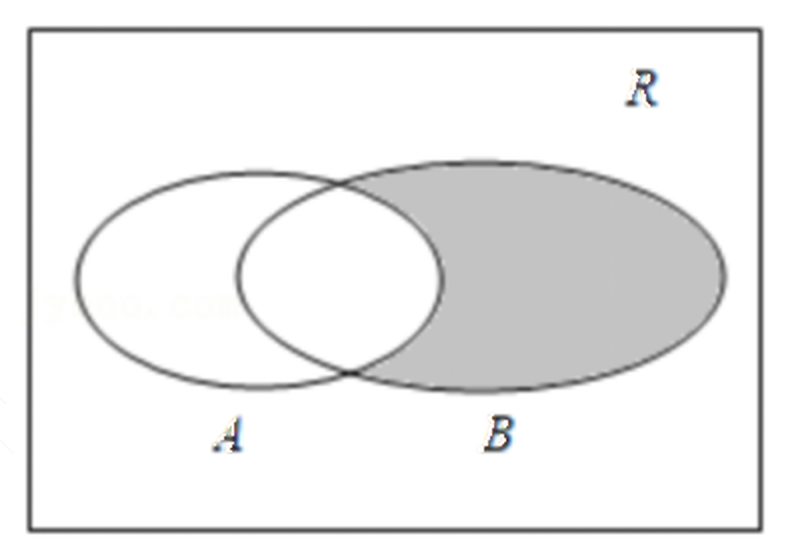
\includegraphics[width=0.36\textwidth]{figures/gao127_q4.png}
\end{center}

\ifanswer
\solbegin
\step{已知 $\R$ 是实数集，集合 $A=\{x\mid 1<x<2\}$, $B=\left\{x\mid 0<x<\frac32\right\}$,}
\step{阴影部分表示的集合是 $\overline A\cap B=\{x\mid 0<x\leqslant1\}$，即 $(0,1]$.}
\solend
\fi

\item 若集合 $\{x\mid (a-1)x^2+3x-2=0\}$ 有且仅有两个子集，则实数 $a$ 的值为\blankline[4.4em].

\ifanswer
\solbegin
\step{由题意得 $\{x\mid (a-1)x^2+3x-2=0\}$ 为单元素集，}
\step{所以 $a-1=0$ 或 $\begin{cases}a-1\neq0\\\triangle=9+8(a-1)=0\end{cases}$，所以 $a=1$ 或 $a=-\frac18$.}
\solend
\fi

\item 已知条件 $\alpha:x\leqslant m$，条件 $\beta:x^2-x\leqslant0$，若 $\alpha$ 是 $\beta$ 的必要条件，则实数 $m$ 的取值范围是为\blankline[4.4em].

\ifanswer
\solbegin
\step{不等式 $x^2-x\leqslant0$ 的解集为 $[0,1]$，}
\step{因为条件 $\alpha:x\leqslant m$，条件 $\beta:x^2-x\leqslant0$，且 $\alpha$ 是 $\beta$ 的必要条件，}
\step{所以集合 $[0,1]$ 是集合 $(-\infty,m]$ 的子集，得 $m\geqslant1$，实数 $m$ 的取值范围是 $[1,+\infty)$.}
\solend
\fi

\item 已知 $\alpha\in\{-2,-1,-\frac12,0,1,2\}$，若幂函数 $y=x^\alpha$ 在 $(0,+\infty)$ 是严格减函数且图像关于 $y$ 轴对称，则 $\alpha=$\blankline[4.4em].

\ifanswer
\solbegin
\step{幂函数 $y=x^\alpha$ 在 $(0,+\infty)$ 是严格减函数，则 $\alpha<0$，且图像关于 $y$ 轴对称，}
\step{则函数为偶函数，故 $\alpha=-2$.}
\solend
\fi

\item 若关于 $x$ 的不等式 $ax^2-3x+2<0$ 的解集不是空集，则实数 $a$ 的取值范围是\blankline[4.4em].

\ifanswer
\solbegin
\step{若 $a>0$，关于 $x$ 的不等式 $ax^2-3x+2<0$ 的解集不空，}
\step{所以一元二次方程 $ax^2-3x+2=0$ 的判别式大于零，}
\step{即 $(-3)^2-8a>0\Rightarrow a<\frac98$，结合 $a>0$ 得 $0<a<\frac98$；}
\step{若 $a\leqslant0$，则关于 $x$ 的不等式 $ax^2-3x+2<0$ 的解集不是空集；}
\step{综上，实数 $a$ 的取值范围是 $\left(-\infty,\frac98\right)$.}
\solend
\fi

\item 设 $\log_{18}2=a$，则 $\log_2 3$ 可用 $a$ 表示为\blankline[4.4em].

\ifanswer
\solbegin
\step{因为 $\log_{18}2=\frac{\log_2 2}{\log_2 18}=\frac1{1+2\log_2 3}=a$，则 $\log_2 3=\frac{1-a}{2a}$.}
\solend
\fi

\item 若关于 $x$ 的不等式 $ax^2+bx+c>0$ 解集为 $\left(-\frac12,3\right)$，则关于 $x$ 的不等式 $cx^2+bx+a<0$ 的解集为\blankline[4.4em].

\ifanswer
\solbegin
\step{由已知得 $a<0$，且 $ax^2+bx+c=a\left(x+\frac12\right)(x-3)$，}
\step{所以 $b=-\frac52 a, c=-\frac32 a$，}
\step{$cx^2+bx+a=-\frac a2(3x-1)(x+2)<0\Leftrightarrow(3x-1)(x+2)<0\Leftrightarrow -2<x<\frac13$，}
\step{故解集为 $\left(-2,\frac13\right)$.}
\solend
\fi

\item 设 $x\in\R$，则方程 $\lvert 2x+3\rvert-\lvert x-2\rvert=\lvert 3x+1\rvert$ 的解集为\blankline[4.4em].

\ifanswer
\solbegin
\step{当 $x\leqslant-\frac32$ 时，原式 $\Leftrightarrow -2x-3+x-2=-3x-1\Leftrightarrow x=2$，不合题意；}
\step{当 $-\frac32<x\leqslant-\frac13$ 时，原式 $\Leftrightarrow 2x+3+x-2=-3x-1\Leftrightarrow x=-\frac13$；}
\step{当 $-\frac13<x\leqslant2$ 时，原式 $\Leftrightarrow 2x+3+x-2=3x+1\Leftrightarrow 1=1$ 即恒成立；}
\step{当 $x>2$ 时，原式 $\Leftrightarrow 2x+3+2-x=3x+1\Leftrightarrow x=2$，不合题意；}
\step{故 $x\in\left[-\frac13,2\right]$.}
\solend
\fi

\item 若关于 $x$ 的不等式 $x^2-4mx+m<0$ 的解集为 $(x_1,x_2)$，若 $x_1>0,x_2>0$，试探究 $x_1+x_2,x_1x_2,x_1^2+x_2^2,\frac1{x_1}+\frac1{x_2}$ 的值，则 $4x_1+x_2$ 的最小值为\blankline[4.4em].

\ifanswer
\solbegin
\step{由题意得方程 $x^2-4mx+m=0$ 有两个相异的正实根 $x_1,x_2$，}
\step{故有 $\begin{cases}\triangle=16m^2-4m>0\\x_1+x_2=4m>0\\x_1\cdot x_2=m>0\end{cases}$，解得 $m>\frac14$，}
\step{则 $x_1^2+x_2^2=(x_1+x_2)^2-2x_1\cdot x_2=16m^2-2m$，$\frac1{x_1}+\frac1{x_2}=\frac{x_1+x_2}{x_1\cdot x_2}=4$，}
\step{则 $4x_1+x_2=\frac14(4x_1+x_2)\left(\frac1{x_1}+\frac1{x_2}\right)=\frac14\left(5+\frac{4x_1}{x_2}+\frac{x_2}{x_1}\right)\geqslant\frac94$，}
\step{当且仅当 $\frac{4x_1}{x_2}=\frac{x_2}{x_1}$ 时，即 $x_2=2x_1$ 时取等号，}
\step{由 $\begin{cases}x_2=2x_1\\\frac1{x_1}+\frac1{x_2}=4\end{cases}$，解得 $\begin{cases}x_1=\frac38\\x_2=\frac34\end{cases}$，于是 $m=x_1\cdot x_2=\frac9{32}\in\left(\frac14,+\infty\right)$，}
\step{即当 $m=\frac9{32}$ 时，$4x_1+x_2$ 取得最小值为 $\frac94$.}
\solend
\fi

\end{enumerate}

\bigsec{二、选择题}

\begin{enumerate}
\setcounter{enumi}{12}

\item 若 $a>0$, $a\neq1$, $M>0$, $N>0$，下列运算正确的是\mbox{（\quad）}

\keepwithprev
A. $\log_a\sqrt[N]{M}=\frac1N\log_a M$\qquad\qquad B. $(\log_a M)^N=N\log_a M$

C. $(\log_a M)\div(\log_a N)=\log_a(M-N)$\qquad\quad D. $\log_a M+\log_a N=\log_a(M+N)$

\ifanswer
\solbegin
\step{对于 $A$，$\log_a\sqrt[N]{M}=\log_a M^{\frac1N}=\frac1N\log_a M$，故 $A$ 正确；}
\step{对于 $B$，$(\log_a M)^N\neq N\log_a M=log_a M^n$，故 $B$ 错误；}
\step{对于 $C$，$(\log_a M)\div(\log_a N)\neq\log_a(M-N)$，故 $C$ 错误；}
\step{对于 $D$，$\log_a M+\log_a N=\log_a MN\neq\log_a(M+N)$，故 $D$ 错误.}
\step{故选 $A$.}
\solend
\fi

\item 下列不等式中正确的是\mbox{（\quad）}

\keepwithprev
A. 若 $a>b$，则 $ac^2>bc^2$\qquad\qquad B. 若 $a<b<0$，则 $a^2<b^2$

C. 若 $1<a<2$ 且 $0<b<3$，则 $1<a+b<5$\qquad D. 若 $\frac1a<1$，则 $a>1$

\ifanswer
\solbegin
\step{$C$ 中 $1+0<a+b<2+3$，即 $1<a+b<5$，正确.}
\step{$A$ 取 $c=0$ 时不成立；$B$ 应为 $a^2>b^2$；$D$ 取 $a=-1$ 时不成立. 故选 $C$.}
\solend
\fi

\item 已知 $y_1=x^3,y_2=x^2$，则下列说法正确的是\mbox{（\quad）}

\keepwithprev
A. $x\in(0,+\infty)$ 时，恒有 $y_1\geqslant y_2$

B. $y_1=x^3$ 与 $y_2=x^2$ 的函数图象仅有唯一交点

C. $x\in(0,1)$ 时，$y_1=x^3$ 图象在 $y_2=x^2$ 图象下方

D. 存在 $x_0\in(1,+\infty)$ 使得 $y_1=y_2$

\ifanswer
\solbegin
\step{$y_1-y_2=x^2(x-1)$，当 $0<x<1$ 时，$y_1<y_2$，故 $C$ 正确，$A$ 错误.}
\step{$y_1=y_2\Leftrightarrow x^2(x-1)=0\Leftrightarrow x=0$ 或 $x=1$，两图象有两个交点，故 $BD$ 错误.}
\step{故选 $C$.}
\solend
\fi

\item 已知非空集合 $A$、$B$ 满足两个条件：(1) $A\cup B=\{1,2,3,4,5,6,7\}$, $A\cap B=\varnothing$；(2) 若 $x\in A$，则 $x+1\in B$，则有序集合对 $(A,B)$ 的个数为\mbox{（\quad）}

\keepwithprev
A. $17$\qquad\qquad B. $18$\qquad\qquad C. $19$\qquad\qquad D. $20$

\ifanswer
\solbegin
\step{当 $A$ 为单元素集合时，有 6 种情况：}
\step{当 $A$ 为双元素集合时，$A=\{1,3\}, A=\{1,4\}, A=\{1,5\}, A=\{1,6\}, A=\{2,4\}$,}
\step{$A=\{2,5\}, A=\{2,6\}, A=\{3,5\}, A=\{3,6\}, A=\{4,6\}$，共 10 种情况；}
\step{当 $A$ 为三元素集合时，$A=\{1,3,5\}, A=\{1,3,6\}, A=\{1,4,6\}, A=\{2,4,6\}$，}
\step{共 4 种情况；}
\step{当 $A$ 为四元素集合时，不成立；}
\step{故有序集合对 $(A,B)$ 的个数为 20，故选 $D$.}
\solend
\fi

\end{enumerate}

\bigsec{三、解答题}

\begin{enumerate}
\setcounter{enumi}{16}

\item 已知 $x,y\in\R$，比较 $x^2+y^2$ 与 $2(2x-y)-5$ 的大小.

\ifanswer
\solbegin
\step{因为 $x^2+y^2-2(2x-y)+5=(x-2)^2+(y+1)^2\geqslant0$，}
\step{所以 $x^2+y^2\geqslant2(2x-y)-5$.}
\solend
\fi

\item 已知集合 $A=\{x\mid x^2+4x=0\}$，$B=\{x\mid x^2+2(a+1)x+a^2-1=0\}$.

(1) 若 $A$ 是 $B$ 的子集，求实数 $a$ 的值；

(2) 若 $B$ 是 $A$ 的子集，求实数 $a$ 的取值范围.

\ifanswer
\solbegin
\step{(1) 因为 $A=\{-4,0\}$，$B=\{x\mid x^2+2(a+1)x+a^2-1=0\}$，又 $A\subseteq B$，}
\step{所以 $A=B$，所以 $\begin{cases}-4+0=-2(a+1)\\-4\times0=a^2-1\end{cases}$，所以 $a=1$；}
\step{(2) 因为 $B$ 是 $A$ 的子集，所以 $B=\varnothing$ 或 $B=\{-4\}$ 或 $B=\{0\}$ 或 $B=\{-4,0\}$，}
\step{① $B=\varnothing$ 时，$\triangle=4(a+1)^2-4(a^2-1)<0$，所以 $a<-1$；}
\step{② $B=\{-4\}$ 时，$\begin{cases}-4+(-4)=-2(a+1)\\-4\times(-4)=a^2-1\end{cases}$，无解；}
\step{③ $B=\{0\}$ 时，$\begin{cases}0+0=-2(a+1)\\0\times0=a^2-1\end{cases}$，所以 $a=-1$；}
\step{④ $B=\{-4,0\}$ 时，由 (1) 得 $a=1$，}
\step{综上，实数 $a$ 的取值范围为 $(-\infty,-1]\cup\{1\}$.}
\solend
\fi

\item 某企业在现有设备下每日生产原先成本 $y$（单位：万元）与日产量 $x$（单位：吨）之间的函数关系式：$y=2x^2+(15-4k)x+120k+8$，近年来各部门都非常重视大气污染防治工作，为了配合环境卫生综合整治，该企业引进了除尘设备，每吨产品的除尘费用为 $k$ 万元，引进除尘设备后，当日产量 $x=1$ 时，总成本（总成本为原先成本和除尘费用之和）为 142 万元.

(1) 求 $k$ 的值；

(2) 求引进除尘设备后日产量为多少时，每吨产品的成本最小，并求出最小值.

\ifanswer
\solbegin
\step{(1) 该企业引进了除尘设备，}
\step{每日生产总成本 $h$（单位：万元）与日产量 $x$（单位：吨）之间的关系为}
\step{$h=2x^2+(15-4k)x+120k+8+kx=2x^2+(15-3k)x+120k+8$，}
\step{当日产量 $x=1$ 时，总成本为 $h=142$ 万元，}
\step{代入得 $2+(15-3k)+120k+8=142\Rightarrow k=1$，}
\step{(2) 由 (1) 得 $h=2x^2+12x+128$，}
\step{所以每吨产品的成本为 $w=\frac{2x^2+12x+128}{x}=2x+\frac{128}{x}+12$}
\step{$\geqslant2\sqrt{2x\cdot\frac{128}{x}}+12=44$，当且仅当 $2x=\frac{128}{x}$，即 $x=8$ 时，取等号，}
\step{所以引进除尘设备后日产量为 8 吨时，每吨产品的成本最小，}
\step{且最小值为 44 万元.}
\solend
\fi

\item 已知集合 $A=\{x\mid \lvert x-a\rvert<2\}$，集合 $B=\left\{x\mid\frac{2x-1}{x+2}<1\right\}$.

(1) 若 $a=2$，求 $A\cup B$；

(2) 若 $A\cap B=A$，求实数 $a$ 的取值范围.

\ifanswer
\solbegin
\step{(1) 若 $a=2$，则 $A=\{x\mid \lvert x-a\rvert<2\}=\{x\mid \lvert x-2\rvert<2\}=\{x\mid 0<x<4\}$，}
\step{由 $\frac{2x-1}{x+2}<1$ 得 $\frac{x-3}{x+2}<0$，即 $(x-3)(x+2)<0$，解得 $-2<x<3$，}
\step{所以 $B=\{x\mid -2<x<3\}$，所以 $A\cup B=\{x\mid -2<x<4\}$；}
\step{(2) 由 (1) 得 $B=\{x\mid -2<x<3\}$，}
\step{$A=\{x\mid \lvert x-a\rvert<2\}=\{x\mid a-2<x<a+2\}$，}
\step{若 $A\cap B=A$，则 $A\subseteq B$，则 $\begin{cases}a-2\geqslant-2\\a+2\leqslant3\end{cases}$，解得 $0\leqslant a\leqslant1$，}
\step{即实数 $a$ 的取值范围为 $[0,1]$.}
\solend
\fi

\item 已知自变量为 $x$ 的函数 $y=\frac{ax+b}{x+a}$，

(1) 若 $a=1$ 且 $b=2$，则函数 $y=\frac{ax+b}{x+a}$ 图像可由幂函数\blankline[4.4em]（写解析式）先沿 $x$ 轴方向\blankline[4.4em]平移\blankline[4.4em]个单位，再沿 $y$ 轴方向向上平移\blankline[4.4em]个单位得到；

(2) 当 $a>0$ 且 $b=-2$ 时不等式 $\frac{ax+b}{x+a}\leqslant\frac{2x^2}{x+a}$ 对 $x>0$ 恒成立，求实数 $a$ 的最大值；

(3) 若 $b=-2$ 且关于 $x$ 的不等式 $x^2\log_2\frac{4(a+1)}a+2x\log_2\frac{2a}{a+1}+\log_2\frac{(a+1)^2}{4a^2}\leqslant0$ 解集是单元素集，求出 $a$ 值，并求出函数 $y=\frac{ax-2}{x+a}$ 的对称中心.

\ifanswer
\solbegin
\step{(1) 已知自变量为 $x$ 的函数 $y=\frac{ax+b}{x+a}$，}
\step{当 $a=1$ 且 $b=2$ 时，$y=\frac{x+2}{x+1}=\frac{x+1+1}{x+1}=1+\frac1{x+1}$，}
\step{由幂函数 $y=\frac1x$，先沿 $x$ 轴方向向左平移一个单位，}
\step{再沿 $y$ 轴方向向上平移一个单位得到；}
\step{(2) 当 $a>0$ 且 $b=-2$ 时不等式 $\frac{ax+b}{x+a}\leqslant\frac{2x^2}{x+a}$ 即 $\frac{ax-2}{x+a}\leqslant\frac{2x^2}{x+a}$ 对 $x>0$ 恒成立，}
\step{因为 $a>0$ 且 $x>0$，所以 $x+a>0$，所以等价于 $ax-2\leqslant2x^2$ 对 $x>0$ 恒成立，}
\step{即 $2x^2-ax+2\geqslant0$ 对 $x>0$ 恒成立，}
\step{因为函数 $g(x)=2x^2-ax+2$ 的对称轴 $x=\frac a4>0$，且 $g(0)=2>0$，}
\step{则 $\begin{cases}\triangle=(-a)^2-4\times2\times2\leqslant0\\a>0\end{cases}$，解得 $0<a\leqslant4$，所以 $a$ 的最大值为 4；}
\step{(3) 关于 $x$ 的不等式 $x^2\log_2\frac{4(a+1)}a+2x\log_2\frac{2a}{a+1}+\log_2\frac{(a+1)^2}{4a^2}\leqslant0$ 解集}
\step{是单元素集，由 $\frac{4(a+1)}a>0$，则 $a>0$ 或 $a<-1$，}
\step{若 $\log_2\frac{4(a+1)}a=0$，则 $\frac{4(a+1)}a=1$，解得 $a=-\frac43$，}
\step{此时不等式为 $6x-6\leqslant0$，解得 $x\leqslant1$，不符合题意，}
\step{若 $\log_2\frac{4(a+1)}a>0$，即 $\frac{4(a+1)}a>1$，解得 $a>0$ 或 $a<-\frac43$，}
\step{则 $\triangle=\left(2\log_2\frac{2a}{a+1}\right)^2-4\log_2\frac{4(a+1)}a\cdot\log_2\frac{(a+1)^2}{4a^2}=0$，}
\step{令 $\log_2\frac{2a}{a+1}=t$，则 $t^2-(3-t)(-2t)=0$，解得 $t=0$ 或 $t=6$，}
\step{当 $\log_2\frac{2a}{a+1}=0$，解得 $a=1$，$\log_2\frac{2a}{a+1}=6$，解得 $a=-\frac{32}{31}$(舍去)，所以 $a=1$，}
\step{则函数 $y=\frac{ax-2}{x+a}$ 即为 $y=\frac{x-2}{x+1}=\frac{x+1-3}{x+1}=1+\frac{-3}{x+1}$，}
\step{对称中心为 $(-1,1)$.}
\solend
\fi

\end{enumerate}

\end{document}
"
%
% 原始材料：微信公众号“魔都数学加油站”文章，作者破晓，2026-11-11 18:35 发布；
% 连载“27学年高一127”，原文标题“27学年高一127——2026-2027年上海市南汇一中高一上期中”；
% 原文链接：https://mp.weixin.qq.com/s/nozIwRgeWSKPCPSiqfCm2Q。
% 正文为 9 张 PNG 页（01、02、03、09 为 2560×3620，04、05、06、07、08 为 4762×6735），
% 题目下印有【解析】，为讲评版。题目、解析均据原图转录；
% 卷面粉红色水印“魔都数学加油站”及公众号页脚未录入。全卷仅第 4 题一幅插图。
% 第 09 页只有一行“对称中心为(-1,1).”及水印，是第 08 页末行的续尾页。
%
% 卷首标题：原卷印作“2026-2027 年南汇一中高一上期中”（公众号标题中的“上海市”
% 卷面标题行没有，本稿照卷面），年份区间按全稿惯例排 en dash；原卷未印副标题，
% 本卷为期中卷、跨三章，按题目内容标为“集合与常用逻辑用语、不等式、函数”
% （第 4/5/6/16/18/20 题为集合与常用逻辑用语，第 8/10/11/12/14/17 题为不等式，
% 第 3/7/9/13/15/19/21 题为函数；与 106、125 同为期中复习卷，口径相同）。
%
% 与原卷的排版差异：
%   ① 原文从第 3 题起，填空题编号为 3—12、选择题为 13—16、解答题为 17—21，本稿保留原题号；
%   ② 原卷每题下直接印【解析】，本稿按全稿惯例置于答案版；四道选择题答案均在解析末句
%      “故选 …”，括号内留空、不另提 \ans{}；全卷无只印【答案】或括号内答案的题；
%   ③ 原卷未印副标题，本稿按“知识模块”口径补出；
%   ④ 原卷填空横线按全稿惯例排为 \blankline[4.4em]；选择题括号排 \mbox{（\quad）}、
%      选项段前按惯例加 \keepwithprev；解答题不留作答区（原卷为讲评版，与 109—125 同）；
%      第 21 题 (1) 的四处填空横线亦排 \blankline[4.4em]；
%   ⑤ 原卷数集排斜体 $R$，按全稿惯例改 \R；绝对值排 \lvert…\rvert，集合描述竖线排 \mid；
%      补集记号照原卷上划线排 \overline{A}；不等号一律 \leqslant / \geqslant；
%   ⑥ 第 4 题插图原在题干右侧，本稿按全稿惯例移至题干之后居中排（取原卷截图、
%      去粉色水印后 2× LANCZOS 放大，存 figures/gao127_q4.png），三版都出；
%      并在该题 \item 前加 \needvspace{} 守卫，把题干与插图整块推走；
%   ⑦ 原卷子题编号 (1)(2)(3) 与括号按全稿惯例排；“（单位：万元）”“（写解析式）”
%      用全角括号，第 21 题 (3) 解析“(舍去)”用半角括号，均照录；
%   ⑧ 第 09 页仅一行“对称中心为(-1,1).”为第 08 页末行之续尾，本稿按原卷印刷行
%      另起一条 \step，置于答案版最后一题解析之末。
%
% 子集符号：第 18 题 (1) 解析 $A\subseteq B$、第 20 题 (2) 解析 $A\subseteq B$ 均印有
%   下划线，照录 \subseteq；全卷无 \subset。回原图放大逐处确认。
%
% 判别式字形：本卷 5 处判别式（第 5 题解析 cases 内 $\triangle=9+8(a-1)=0$、
%   第 12 题解析 cases 内 $\triangle=16m^2-4m>0$、第 18 题① $\triangle=4(a+1)^2-4(a^2-1)<0$、
%   第 21 题 (2) cases 内 $\triangle=(-a)^2-4\times2\times2\leqslant0$、
%   第 21 题 (3) $\triangle=\left(2\log_2\frac{2a}{a+1}\right)^2-\cdots=0$）均排等边扁三角，
%   照录 \triangle；逐处回原图全分辨率放大确认，无高三角 $\Delta$（与 高一26 排 $\Delta$ 不同）。
%
% 原卷存疑照录：
%   第 6 题题干作“则实数 $m$ 的取值范围是为____”（“是为”叠用，疑衍一字），照录；
%   第 12 题题干“试探究 $x_1+x_2, x_1x_2, x_1^2+x_2^2, \frac1{x_1}+\frac1{x_2}$ 的值，
%     则 $4x_1+x_2$ 的最小值为____”与后文衔接突兀，照录；
%   第 13 题解析 B 作“$(\log_a M)^N\neq N\log_a M=log_a M^n$”，后一 log 为斜体、
%     指数作小写 $n$，与前式 $N\log_a M$ 及题干 $N$ 不一致，照录；
%   第 13 题解析 A、B、C 三步句末用“；”，D 步句末用“.”，标点不一致，照录；
%   第 15 题解析“故 $BD$ 错误.”两选项字母连写、无顿号，照录；
%   第 7 题题干及解析用“图像”，第 15 题 B、C 及解析用“图象”，全卷两种写法混用，照录未统一；
%   第 21 题 (3) 题干“求出 $a$ 值”（通常作“求出 $a$ 的值”），照录；
%   第 21 题 (3) 解析“解得 $a=1$，$\log_2\frac{2a}{a+1}=6$，解得 $a=-\frac{32}{31}$(舍去)，
%     所以 $a=1$”两个“解得”并列、且舍去值用半角括号，照录；
%   第 09 页“对称中心为(-1,1).”用半角括号与半角句点，照录；
%   第 8 题解析“若 $a\leqslant0$，则关于 $x$ 的不等式 $ax^2-3x+2<0$ 的解集不是空集；”
%     未给理由直接断言，照录；
%   第 18 题 (1) 由 $A\subseteq B$ 直接得 $A=B$，照录。
%
% 行数核对：逐题数 \step 条数，合计 95 条（Q3：1；Q4：2；Q5：2；Q6：3；Q7：2；
% Q8：5；Q9：1；Q10：4；Q11：5；Q12：7；Q13：5；Q14：2；Q15：3；Q16：7；
% Q17：2；Q18：8；Q19：10；Q20：7；Q21：19），与原卷印刷行逐题相等
% （cases 块作一个印刷行计；Q21 第 19 行为第 09 页续尾）。全卷 19 题均印【解析】，
% 无只印【答案】或括号内答案的题，故 \ans{} 为 0；四道选择题括号内留空、不另提 \ans{}。
%
\documentclass[a4paper,11pt]{article}
\usepackage{common}

\begin{document}

\examtitlest[3]{2026--2027 年南汇一中高一上期中}{集合与常用逻辑用语、不等式、函数}

\bigsec{一、填空题}

\begin{enumerate}
\setcounter{enumi}{2}

\item 把 $\sqrt[4]{a\sqrt a}(a>0)$ 化成有理数指数幂的形式为\blankline[4.4em].

\ifanswer
\solbegin
\step{$\sqrt[4]{a\sqrt a}=(a\cdot a^{\frac12})^{\frac14}=a^{\frac38}$.}
\solend
\fi

\needvspace{6.5cm}
\item 已知集合 $A=\{x\mid 1<x<2\}$, $B=\left\{x\mid 0<x<\frac32\right\}$, 则如图阴影部分表示的集合是\blankline[4.4em].

\begin{center}
% 图取原卷截图（第 1 页题干右侧）、去水印后 2× LANCZOS 放大，本稿移至题干之后
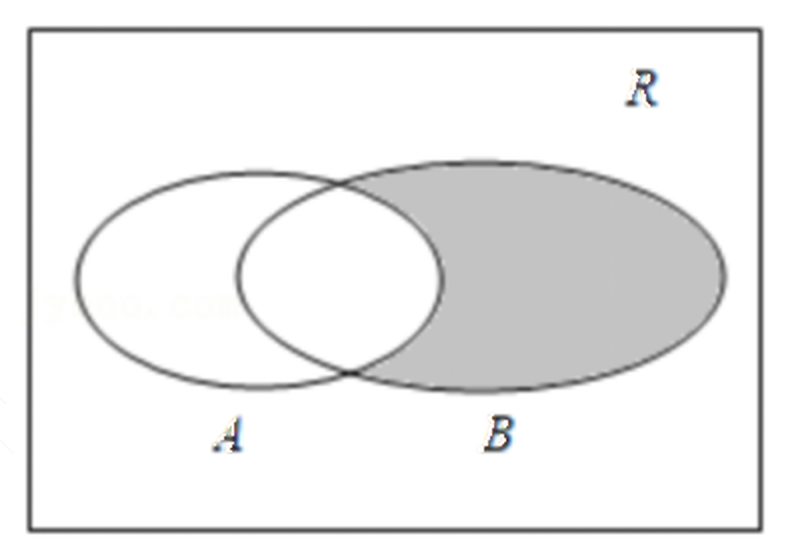
\includegraphics[width=0.36\textwidth]{figures/gao127_q4.png}
\end{center}

\ifanswer
\solbegin
\step{已知 $\R$ 是实数集，集合 $A=\{x\mid 1<x<2\}$, $B=\left\{x\mid 0<x<\frac32\right\}$,}
\step{阴影部分表示的集合是 $\overline A\cap B=\{x\mid 0<x\leqslant1\}$，即 $(0,1]$.}
\solend
\fi

\item 若集合 $\{x\mid (a-1)x^2+3x-2=0\}$ 有且仅有两个子集，则实数 $a$ 的值为\blankline[4.4em].

\ifanswer
\solbegin
\step{由题意得 $\{x\mid (a-1)x^2+3x-2=0\}$ 为单元素集，}
\step{所以 $a-1=0$ 或 $\begin{cases}a-1\neq0\\\triangle=9+8(a-1)=0\end{cases}$，所以 $a=1$ 或 $a=-\frac18$.}
\solend
\fi

\item 已知条件 $\alpha:x\leqslant m$，条件 $\beta:x^2-x\leqslant0$，若 $\alpha$ 是 $\beta$ 的必要条件，则实数 $m$ 的取值范围是为\blankline[4.4em].

\ifanswer
\solbegin
\step{不等式 $x^2-x\leqslant0$ 的解集为 $[0,1]$，}
\step{因为条件 $\alpha:x\leqslant m$，条件 $\beta:x^2-x\leqslant0$，且 $\alpha$ 是 $\beta$ 的必要条件，}
\step{所以集合 $[0,1]$ 是集合 $(-\infty,m]$ 的子集，得 $m\geqslant1$，实数 $m$ 的取值范围是 $[1,+\infty)$.}
\solend
\fi

\item 已知 $\alpha\in\{-2,-1,-\frac12,0,1,2\}$，若幂函数 $y=x^\alpha$ 在 $(0,+\infty)$ 是严格减函数且图像关于 $y$ 轴对称，则 $\alpha=$\blankline[4.4em].

\ifanswer
\solbegin
\step{幂函数 $y=x^\alpha$ 在 $(0,+\infty)$ 是严格减函数，则 $\alpha<0$，且图像关于 $y$ 轴对称，}
\step{则函数为偶函数，故 $\alpha=-2$.}
\solend
\fi

\item 若关于 $x$ 的不等式 $ax^2-3x+2<0$ 的解集不是空集，则实数 $a$ 的取值范围是\blankline[4.4em].

\ifanswer
\solbegin
\step{若 $a>0$，关于 $x$ 的不等式 $ax^2-3x+2<0$ 的解集不空，}
\step{所以一元二次方程 $ax^2-3x+2=0$ 的判别式大于零，}
\step{即 $(-3)^2-8a>0\Rightarrow a<\frac98$，结合 $a>0$ 得 $0<a<\frac98$；}
\step{若 $a\leqslant0$，则关于 $x$ 的不等式 $ax^2-3x+2<0$ 的解集不是空集；}
\step{综上，实数 $a$ 的取值范围是 $\left(-\infty,\frac98\right)$.}
\solend
\fi

\item 设 $\log_{18}2=a$，则 $\log_2 3$ 可用 $a$ 表示为\blankline[4.4em].

\ifanswer
\solbegin
\step{因为 $\log_{18}2=\frac{\log_2 2}{\log_2 18}=\frac1{1+2\log_2 3}=a$，则 $\log_2 3=\frac{1-a}{2a}$.}
\solend
\fi

\item 若关于 $x$ 的不等式 $ax^2+bx+c>0$ 解集为 $\left(-\frac12,3\right)$，则关于 $x$ 的不等式 $cx^2+bx+a<0$ 的解集为\blankline[4.4em].

\ifanswer
\solbegin
\step{由已知得 $a<0$，且 $ax^2+bx+c=a\left(x+\frac12\right)(x-3)$，}
\step{所以 $b=-\frac52 a, c=-\frac32 a$，}
\step{$cx^2+bx+a=-\frac a2(3x-1)(x+2)<0\Leftrightarrow(3x-1)(x+2)<0\Leftrightarrow -2<x<\frac13$，}
\step{故解集为 $\left(-2,\frac13\right)$.}
\solend
\fi

\item 设 $x\in\R$，则方程 $\lvert 2x+3\rvert-\lvert x-2\rvert=\lvert 3x+1\rvert$ 的解集为\blankline[4.4em].

\ifanswer
\solbegin
\step{当 $x\leqslant-\frac32$ 时，原式 $\Leftrightarrow -2x-3+x-2=-3x-1\Leftrightarrow x=2$，不合题意；}
\step{当 $-\frac32<x\leqslant-\frac13$ 时，原式 $\Leftrightarrow 2x+3+x-2=-3x-1\Leftrightarrow x=-\frac13$；}
\step{当 $-\frac13<x\leqslant2$ 时，原式 $\Leftrightarrow 2x+3+x-2=3x+1\Leftrightarrow 1=1$ 即恒成立；}
\step{当 $x>2$ 时，原式 $\Leftrightarrow 2x+3+2-x=3x+1\Leftrightarrow x=2$，不合题意；}
\step{故 $x\in\left[-\frac13,2\right]$.}
\solend
\fi

\item 若关于 $x$ 的不等式 $x^2-4mx+m<0$ 的解集为 $(x_1,x_2)$，若 $x_1>0,x_2>0$，试探究 $x_1+x_2,x_1x_2,x_1^2+x_2^2,\frac1{x_1}+\frac1{x_2}$ 的值，则 $4x_1+x_2$ 的最小值为\blankline[4.4em].

\ifanswer
\solbegin
\step{由题意得方程 $x^2-4mx+m=0$ 有两个相异的正实根 $x_1,x_2$，}
\step{故有 $\begin{cases}\triangle=16m^2-4m>0\\x_1+x_2=4m>0\\x_1\cdot x_2=m>0\end{cases}$，解得 $m>\frac14$，}
\step{则 $x_1^2+x_2^2=(x_1+x_2)^2-2x_1\cdot x_2=16m^2-2m$，$\frac1{x_1}+\frac1{x_2}=\frac{x_1+x_2}{x_1\cdot x_2}=4$，}
\step{则 $4x_1+x_2=\frac14(4x_1+x_2)\left(\frac1{x_1}+\frac1{x_2}\right)=\frac14\left(5+\frac{4x_1}{x_2}+\frac{x_2}{x_1}\right)\geqslant\frac94$，}
\step{当且仅当 $\frac{4x_1}{x_2}=\frac{x_2}{x_1}$ 时，即 $x_2=2x_1$ 时取等号，}
\step{由 $\begin{cases}x_2=2x_1\\\frac1{x_1}+\frac1{x_2}=4\end{cases}$，解得 $\begin{cases}x_1=\frac38\\x_2=\frac34\end{cases}$，于是 $m=x_1\cdot x_2=\frac9{32}\in\left(\frac14,+\infty\right)$，}
\step{即当 $m=\frac9{32}$ 时，$4x_1+x_2$ 取得最小值为 $\frac94$.}
\solend
\fi

\end{enumerate}

\bigsec{二、选择题}

\begin{enumerate}
\setcounter{enumi}{12}

\item 若 $a>0$, $a\neq1$, $M>0$, $N>0$，下列运算正确的是\mbox{（\quad）}

\keepwithprev
A. $\log_a\sqrt[N]{M}=\frac1N\log_a M$\qquad\qquad B. $(\log_a M)^N=N\log_a M$

C. $(\log_a M)\div(\log_a N)=\log_a(M-N)$\qquad\quad D. $\log_a M+\log_a N=\log_a(M+N)$

\ifanswer
\solbegin
\step{对于 $A$，$\log_a\sqrt[N]{M}=\log_a M^{\frac1N}=\frac1N\log_a M$，故 $A$ 正确；}
\step{对于 $B$，$(\log_a M)^N\neq N\log_a M=log_a M^n$，故 $B$ 错误；}
\step{对于 $C$，$(\log_a M)\div(\log_a N)\neq\log_a(M-N)$，故 $C$ 错误；}
\step{对于 $D$，$\log_a M+\log_a N=\log_a MN\neq\log_a(M+N)$，故 $D$ 错误.}
\step{故选 $A$.}
\solend
\fi

\item 下列不等式中正确的是\mbox{（\quad）}

\keepwithprev
A. 若 $a>b$，则 $ac^2>bc^2$\qquad\qquad B. 若 $a<b<0$，则 $a^2<b^2$

C. 若 $1<a<2$ 且 $0<b<3$，则 $1<a+b<5$\qquad D. 若 $\frac1a<1$，则 $a>1$

\ifanswer
\solbegin
\step{$C$ 中 $1+0<a+b<2+3$，即 $1<a+b<5$，正确.}
\step{$A$ 取 $c=0$ 时不成立；$B$ 应为 $a^2>b^2$；$D$ 取 $a=-1$ 时不成立. 故选 $C$.}
\solend
\fi

\item 已知 $y_1=x^3,y_2=x^2$，则下列说法正确的是\mbox{（\quad）}

\keepwithprev
A. $x\in(0,+\infty)$ 时，恒有 $y_1\geqslant y_2$

B. $y_1=x^3$ 与 $y_2=x^2$ 的函数图象仅有唯一交点

C. $x\in(0,1)$ 时，$y_1=x^3$ 图象在 $y_2=x^2$ 图象下方

D. 存在 $x_0\in(1,+\infty)$ 使得 $y_1=y_2$

\ifanswer
\solbegin
\step{$y_1-y_2=x^2(x-1)$，当 $0<x<1$ 时，$y_1<y_2$，故 $C$ 正确，$A$ 错误.}
\step{$y_1=y_2\Leftrightarrow x^2(x-1)=0\Leftrightarrow x=0$ 或 $x=1$，两图象有两个交点，故 $BD$ 错误.}
\step{故选 $C$.}
\solend
\fi

\item 已知非空集合 $A$、$B$ 满足两个条件：(1) $A\cup B=\{1,2,3,4,5,6,7\}$, $A\cap B=\varnothing$；(2) 若 $x\in A$，则 $x+1\in B$，则有序集合对 $(A,B)$ 的个数为\mbox{（\quad）}

\keepwithprev
A. $17$\qquad\qquad B. $18$\qquad\qquad C. $19$\qquad\qquad D. $20$

\ifanswer
\solbegin
\step{当 $A$ 为单元素集合时，有 6 种情况：}
\step{当 $A$ 为双元素集合时，$A=\{1,3\}, A=\{1,4\}, A=\{1,5\}, A=\{1,6\}, A=\{2,4\}$,}
\step{$A=\{2,5\}, A=\{2,6\}, A=\{3,5\}, A=\{3,6\}, A=\{4,6\}$，共 10 种情况；}
\step{当 $A$ 为三元素集合时，$A=\{1,3,5\}, A=\{1,3,6\}, A=\{1,4,6\}, A=\{2,4,6\}$，}
\step{共 4 种情况；}
\step{当 $A$ 为四元素集合时，不成立；}
\step{故有序集合对 $(A,B)$ 的个数为 20，故选 $D$.}
\solend
\fi

\end{enumerate}

\bigsec{三、解答题}

\begin{enumerate}
\setcounter{enumi}{16}

\item 已知 $x,y\in\R$，比较 $x^2+y^2$ 与 $2(2x-y)-5$ 的大小.

\ifanswer
\solbegin
\step{因为 $x^2+y^2-2(2x-y)+5=(x-2)^2+(y+1)^2\geqslant0$，}
\step{所以 $x^2+y^2\geqslant2(2x-y)-5$.}
\solend
\fi

\item 已知集合 $A=\{x\mid x^2+4x=0\}$，$B=\{x\mid x^2+2(a+1)x+a^2-1=0\}$.

(1) 若 $A$ 是 $B$ 的子集，求实数 $a$ 的值；

(2) 若 $B$ 是 $A$ 的子集，求实数 $a$ 的取值范围.

\ifanswer
\solbegin
\step{(1) 因为 $A=\{-4,0\}$，$B=\{x\mid x^2+2(a+1)x+a^2-1=0\}$，又 $A\subseteq B$，}
\step{所以 $A=B$，所以 $\begin{cases}-4+0=-2(a+1)\\-4\times0=a^2-1\end{cases}$，所以 $a=1$；}
\step{(2) 因为 $B$ 是 $A$ 的子集，所以 $B=\varnothing$ 或 $B=\{-4\}$ 或 $B=\{0\}$ 或 $B=\{-4,0\}$，}
\step{① $B=\varnothing$ 时，$\triangle=4(a+1)^2-4(a^2-1)<0$，所以 $a<-1$；}
\step{② $B=\{-4\}$ 时，$\begin{cases}-4+(-4)=-2(a+1)\\-4\times(-4)=a^2-1\end{cases}$，无解；}
\step{③ $B=\{0\}$ 时，$\begin{cases}0+0=-2(a+1)\\0\times0=a^2-1\end{cases}$，所以 $a=-1$；}
\step{④ $B=\{-4,0\}$ 时，由 (1) 得 $a=1$，}
\step{综上，实数 $a$ 的取值范围为 $(-\infty,-1]\cup\{1\}$.}
\solend
\fi

\item 某企业在现有设备下每日生产原先成本 $y$（单位：万元）与日产量 $x$（单位：吨）之间的函数关系式：$y=2x^2+(15-4k)x+120k+8$，近年来各部门都非常重视大气污染防治工作，为了配合环境卫生综合整治，该企业引进了除尘设备，每吨产品的除尘费用为 $k$ 万元，引进除尘设备后，当日产量 $x=1$ 时，总成本（总成本为原先成本和除尘费用之和）为 142 万元.

(1) 求 $k$ 的值；

(2) 求引进除尘设备后日产量为多少时，每吨产品的成本最小，并求出最小值.

\ifanswer
\solbegin
\step{(1) 该企业引进了除尘设备，}
\step{每日生产总成本 $h$（单位：万元）与日产量 $x$（单位：吨）之间的关系为}
\step{$h=2x^2+(15-4k)x+120k+8+kx=2x^2+(15-3k)x+120k+8$，}
\step{当日产量 $x=1$ 时，总成本为 $h=142$ 万元，}
\step{代入得 $2+(15-3k)+120k+8=142\Rightarrow k=1$，}
\step{(2) 由 (1) 得 $h=2x^2+12x+128$，}
\step{所以每吨产品的成本为 $w=\frac{2x^2+12x+128}{x}=2x+\frac{128}{x}+12$}
\step{$\geqslant2\sqrt{2x\cdot\frac{128}{x}}+12=44$，当且仅当 $2x=\frac{128}{x}$，即 $x=8$ 时，取等号，}
\step{所以引进除尘设备后日产量为 8 吨时，每吨产品的成本最小，}
\step{且最小值为 44 万元.}
\solend
\fi

\item 已知集合 $A=\{x\mid \lvert x-a\rvert<2\}$，集合 $B=\left\{x\mid\frac{2x-1}{x+2}<1\right\}$.

(1) 若 $a=2$，求 $A\cup B$；

(2) 若 $A\cap B=A$，求实数 $a$ 的取值范围.

\ifanswer
\solbegin
\step{(1) 若 $a=2$，则 $A=\{x\mid \lvert x-a\rvert<2\}=\{x\mid \lvert x-2\rvert<2\}=\{x\mid 0<x<4\}$，}
\step{由 $\frac{2x-1}{x+2}<1$ 得 $\frac{x-3}{x+2}<0$，即 $(x-3)(x+2)<0$，解得 $-2<x<3$，}
\step{所以 $B=\{x\mid -2<x<3\}$，所以 $A\cup B=\{x\mid -2<x<4\}$；}
\step{(2) 由 (1) 得 $B=\{x\mid -2<x<3\}$，}
\step{$A=\{x\mid \lvert x-a\rvert<2\}=\{x\mid a-2<x<a+2\}$，}
\step{若 $A\cap B=A$，则 $A\subseteq B$，则 $\begin{cases}a-2\geqslant-2\\a+2\leqslant3\end{cases}$，解得 $0\leqslant a\leqslant1$，}
\step{即实数 $a$ 的取值范围为 $[0,1]$.}
\solend
\fi

\item 已知自变量为 $x$ 的函数 $y=\frac{ax+b}{x+a}$，

(1) 若 $a=1$ 且 $b=2$，则函数 $y=\frac{ax+b}{x+a}$ 图像可由幂函数\blankline[4.4em]（写解析式）先沿 $x$ 轴方向\blankline[4.4em]平移\blankline[4.4em]个单位，再沿 $y$ 轴方向向上平移\blankline[4.4em]个单位得到；

(2) 当 $a>0$ 且 $b=-2$ 时不等式 $\frac{ax+b}{x+a}\leqslant\frac{2x^2}{x+a}$ 对 $x>0$ 恒成立，求实数 $a$ 的最大值；

(3) 若 $b=-2$ 且关于 $x$ 的不等式 $x^2\log_2\frac{4(a+1)}a+2x\log_2\frac{2a}{a+1}+\log_2\frac{(a+1)^2}{4a^2}\leqslant0$ 解集是单元素集，求出 $a$ 值，并求出函数 $y=\frac{ax-2}{x+a}$ 的对称中心.

\ifanswer
\solbegin
\step{(1) 已知自变量为 $x$ 的函数 $y=\frac{ax+b}{x+a}$，}
\step{当 $a=1$ 且 $b=2$ 时，$y=\frac{x+2}{x+1}=\frac{x+1+1}{x+1}=1+\frac1{x+1}$，}
\step{由幂函数 $y=\frac1x$，先沿 $x$ 轴方向向左平移一个单位，}
\step{再沿 $y$ 轴方向向上平移一个单位得到；}
\step{(2) 当 $a>0$ 且 $b=-2$ 时不等式 $\frac{ax+b}{x+a}\leqslant\frac{2x^2}{x+a}$ 即 $\frac{ax-2}{x+a}\leqslant\frac{2x^2}{x+a}$ 对 $x>0$ 恒成立，}
\step{因为 $a>0$ 且 $x>0$，所以 $x+a>0$，所以等价于 $ax-2\leqslant2x^2$ 对 $x>0$ 恒成立，}
\step{即 $2x^2-ax+2\geqslant0$ 对 $x>0$ 恒成立，}
\step{因为函数 $g(x)=2x^2-ax+2$ 的对称轴 $x=\frac a4>0$，且 $g(0)=2>0$，}
\step{则 $\begin{cases}\triangle=(-a)^2-4\times2\times2\leqslant0\\a>0\end{cases}$，解得 $0<a\leqslant4$，所以 $a$ 的最大值为 4；}
\step{(3) 关于 $x$ 的不等式 $x^2\log_2\frac{4(a+1)}a+2x\log_2\frac{2a}{a+1}+\log_2\frac{(a+1)^2}{4a^2}\leqslant0$ 解集}
\step{是单元素集，由 $\frac{4(a+1)}a>0$，则 $a>0$ 或 $a<-1$，}
\step{若 $\log_2\frac{4(a+1)}a=0$，则 $\frac{4(a+1)}a=1$，解得 $a=-\frac43$，}
\step{此时不等式为 $6x-6\leqslant0$，解得 $x\leqslant1$，不符合题意，}
\step{若 $\log_2\frac{4(a+1)}a>0$，即 $\frac{4(a+1)}a>1$，解得 $a>0$ 或 $a<-\frac43$，}
\step{则 $\triangle=\left(2\log_2\frac{2a}{a+1}\right)^2-4\log_2\frac{4(a+1)}a\cdot\log_2\frac{(a+1)^2}{4a^2}=0$，}
\step{令 $\log_2\frac{2a}{a+1}=t$，则 $t^2-(3-t)(-2t)=0$，解得 $t=0$ 或 $t=6$，}
\step{当 $\log_2\frac{2a}{a+1}=0$，解得 $a=1$，$\log_2\frac{2a}{a+1}=6$，解得 $a=-\frac{32}{31}$(舍去)，所以 $a=1$，}
\step{则函数 $y=\frac{ax-2}{x+a}$ 即为 $y=\frac{x-2}{x+1}=\frac{x+1-3}{x+1}=1+\frac{-3}{x+1}$，}
\step{对称中心为 $(-1,1)$.}
\solend
\fi

\end{enumerate}

\end{document}
